%%%%%%%%%%%%%%%%%%%%%%%%%%%%%%%%%%%%%%%%%%%%%%%%%%%%%%%%%%%%%%%%%
% Contents: Main Input File of the LaTeX2e Introduction
% $Id$
%%%%%%%%%%%%%%%%%%%%%%%%%%%%%%%%%%%%%%%%%%%%%%%%%%%%%%%%%%%%%%%%%
% lshort.tex - The not so short introduction to LaTeX   
%                                                      by Tobias Oetiker
%                                                     oetiker@ee.ethz.ch
%
%                           based on LKURTZ.TEX Uni Graz & TU Wien, 1987
%-----------------------------------------------------------------------
%
% To compile lshort, you need TeX 3.x, LaTeX and makeindex
%
% The sources files of the Intro are:
%      lshort.tex (this file),
%      titel.tex, contrib.tex, biblio.tex
%      things.tex, typeset.tex, math.tex, lssym.tex, spec.tex,
%      lshort.sty, fancyheadings.sty
%
% Further the  verbatim.sty and the layout.sty 
% from the LaTeX Tools distribution is
% required.
%
%
% To print the AMS symbols you need the AMS fonts and the packages
% amsfonts, eufrak and eucal from (AMS LaTeX 1.2)
%
% ---------------------------------------------------------------------

%%%%%%%%%%%%%%%%%%%%%%%%%%%%%%%%%%%%%%%%%%%%%%%%%%%%%%%%%%%%%%%%%
% Contents: Who contributed to this Document
% $Id$
%%%%%%%%%%%%%%%%%%%%%%%%%%%%%%%%%%%%%%%%%%%%%%%%%%%%%%%%%%%%%%%%%
\begin{small}
  \noindent Copyright \copyright{}1995--2021 Tobias Oetiker and Contributors.  All rights reserved.

  This document is free; you can redistribute it and/or modify it
  under the terms of the GNU General Public License as published by
  the Free Software Foundation; either version 2 of the License, or
  (at your option) any later version.

  This document is distributed in the hope that it will be useful, but
  \emph{without any warranty}; without even the implied warranty of
  \emph{merchantability} or \emph{fitness for a particular purpose}\@.  See the GNU
  General Public License for more details.

  You should have received a copy of the GNU General Public License
  along with this document; if not, write to the Free Software
  Foundation, Inc., 51 Franklin Street, Fifth Floor, Boston, MA 02110-1301, %chktex 8
  USA\@.

  \vspace{\stretch{1}}
  \noindent The full text of the GNU General Public License can be found in Appendix~\ref{gplfull} on page~\pageref{gplfull}.
\end{small}

\chapter{Thank you!}
\noindent Much of the material used in this introduction comes from an
Austrian introduction to \LaTeX\ 2.09 written in German by:
\begin{verse}
  \contrib{Hubert Partl}{partl@mail.boku.ac.at}%
  {Zentraler Informatikdienst der Universit\"at f\"ur Bodenkultur Wien}
  \contrib{Irene Hyna}{Irene.Hyna@bmwf.ac.at}%
  {Bundesministerium f\"ur Wissenschaft und Forschung Wien}
  \contrib{Elisabeth Schlegl}{no email}%
  {in Graz}
\end{verse}

If you are interested in the German document, you can find a version
updated for \LaTeXe{} by J\"org Knappen at
\CTAN|info/lshort/german|

\newpage \noindent The
following individuals helped with corrections, suggestions and
material to improve this paper. They put in a big effort to help me
get this document into its present shape. I would like to
sincerely thank all of them. Naturally, all the mistakes you'll find
in this book are mine. If you ever find a word that is spelled
correctly, it must have been one of the people below dropping me a
line.

If you want to contribute to this booklet, you can find all the source code
on \url{https://github.com/oetiker/lshort}. Your pull requests will be
appreciated.

\begin{FlushLeft}
  \small
  Eric~Abrahamsen,        % <eric@ericabrahamsen.net>
  Lenimar~Nunes~de~Andrade, % <lenimar@mat.ufpb.br> 12 Nov 1999
  Eilinger~August,        % <eaugust@student.ethz.ch>
  Rosemary~Bailey,        % <r.a.bailey@qmw.ac.uk> 0.2
  Barbara~Beeton,         % <bnb@ams.org>
  Marc~Bevand,            % <bevand_m@epita.fr>
  Connor~Blakey,          % it's Ligatures!
  Salvatore~Bonaccorso,   % <bonaccos@ee.ethz.ch>
  Pietro~Braione,         % <braione@elet.polimi.it>
  Friedemann~Brauer,      % <fbrauer@is.dal.ca> 3.4
  Markus~Br\"uhwiler,     % <m.br@switzerland.org>
  Jan~Busa,               % <busaj@ccsun.tuke.sk>
  David~Carlisle,         % GONE <carlisle@cs.man.ac.uk> 1.0
  Neil~Carter,            % <n.carter@Swansea.ac.uk>
  Carl~Cerecke,           % <cdc@cosc.canterbury.ac.nz>
  Mike~Chapman,           % <chapman@eeh.ee.ethz.ch> 3.16
  Pierre~Chardaire,       % <pc@sys.uea.ac.uk>
  Xingyou~Chen,           % <niatlantice@gmail.com> 5.04
  Christopher~Chin,       % <chris.chin@rmit.edu.au> 3.1
  Diego~Clavadetscher,    % <dc@clavatax.ch>
  Wim~van~Dam,            % GONE <wimvdam@cs.kun.nl> 2.2
  Benjamin~Deschwanden    % <vdeschwb@student.ethz.ch>
  Jan~Dittberner,         % <jan@jan-dittberner.de> 3.15
  Michael~John~Downes,    % <mjd@ams.org> 14 Oct 1999
  Matthias~Dreier,        % <dreier@ostium.ch>
  David~Dureisseix,       % <dureisse@lmt.ens-cachan.fr> 1.1
  Hans~Ehrbar,            % <ehrbar@econ.utah.edu>
  Elliot,                 % GONE <enh-a@minster.york.ac.uk> 1.1
  Rockrush~Engch,         % <niatlantice@gmail.com>
  William~Faulk,          % <wfaulk@webassign.net>
  Robin~Fairbairns,       % <robin.fairbairns@cl.cam.ac.uk> 0.2 1.0
  Johan~Falk,             % <johan@vaxjonexus.com> 5.0.1
  J\"org~Fischer,         % <j.fischer@xpoint.at> 3.16
  Frank~Fischli,          % <fischlifaenger@gmx.ch>
  Daniel~Flipo,           % <daniel.flipo@univ-lille1.fr>
  Frank,                  % <frank@freezone.co.uk> 11 Feb 2000
  Mic~Milic~Frederickx,   % <mic.milic@web.de>
  David~Frey,             % <david@eos.lugs.ch> 2.2
  Erik~Frisk,             % <frisk@isy.liu.se> 3.4
  Hans~Fugal,             % <hans@fugal.net>
  Robert~Funnell,         % <robert.funnell@mcgill.ca> 5.1
  Greg~Gamble,            % <gregg@maths.uwa.edu.au> 2.2
  Andy~Goth,              % <unununium@openverse.com>
  Cyril~Goutte,           % <goutte@ei.dtu.dk> 2.1 2.2
  Kasper~B.~Graversen,    % <kbg@dkik.dk>
  Arlo~Griffiths,         % <a.griffiths@let.leidenuniv.nl>
  Alexandre~Guimond,      % <guimond@iro.umontreal.ca> 0.9
  Neil~Hammond,           % <nfh@dmu.ac.uk> 0.3
  Christoph~Hamburger,    % <ch.hamburger@gmail.com>
  Rasmus~Borup~Hansen,    % GONE <rbhfamos@math.ku.dk> 0.2 0.9 0.91 0.92 1.9.9
  Joseph~Hilferty,        % <hilferty@fil.ub.es>
  Daniel~Hirsbrunner,     % <dhirsbrunner1@gmail.com>
  Martien~Hulsen,         % <m.a.hulsen@Wbmt.tudelft.nl> 1.0 1.1
  Bj\"orn Hvittfeldt,     % <bjorn@hvittfeldt.com> 3.13
  Morten~H\o gholm,       % <morten.hoegholm@latex-project.org>
  Werner~Icking,          % <werner.icking@gmd.de> 3.1
  Eric~Jacoboni,          % GONE <jacoboni@enseeiht.fr> 0.1 0.9
  Jakob,                  % <diness@get2net.dk>
  Alan~Jeffrey,           % <alanje@cogs.sussex.ac.uk> 0.2
  Martin~Jenkins,         % xqp.ltd@gmail.com 5.04
  Byron~Jones,            % <bj@dmu.ac.uk> 1.1
  David~Jones,            % GONE <djones@ca.mcmaster.dcss.insight> 1.1
  Johannes-Maria~Kaltenbach, % <kaltenbach@zeiss.de> 3.01
  Nils~Kanning,           % <nils@kanning.de>
  Andrzej~Kawalec,        % GONE <akawalec@prz.rzeszow.pl> 1.9.9
  Christian~Kern,         % <ck@unixen.hrz.uni-oldenburg.de> 2.1
  Alain~Kessi,            % <alain_kessi@hotmail.com> 2.2
  Axel~Kielhorn,          % <a.kielhorn@web.de>
  Sander~de~Kievit,       % <Skievit@ucu.uu.nl>
  Kjetil~Kjernsmo,        % <kjetil.kjernsmo@astro.uio.no> 3.2
  Tobias~Klauser,		% <tklauser@access.unizh.ch> 4.17
  J\"org~Knappen,         % <knappen@vkpmzd.kph.uni-mainz.de> 0.1
  Michael~Koundouros,     % <mkoundouros@hotmail.com>
  Matt~Kraai,             % <matt.kraai@amo.abbott.com>
  Tobias~Krewer,          % <tobias.krewer@googlemail.com>
  Flori~Lambrechts,       % <f.lambrechts@softhome.net>
  Mike~Lee,               % <rmrstar@gmail.com>
  Maik~Lehradt,           % <greek@uni-paderborn.de> 0.1
  R\'emi~Letot,           % <r_letot@yahoo.com>
  Axel~Liljencrantz,	% <axel.liljencrantz@byv.kth.se>
  Jasper~Loy,             % <jasper.loy@gmail.com>
  Johan~Lundberg,         % <p99jlu@physto.se>
  Martin~Maechler,        % <maechler@stat.math.ethz.ch> 2.2
  Alexander~Mai,          % <alexander.mai@physik.tu-darmstadt.de> 3.8
  Claus~Malten,           % GONE <asi138%bitnet.djukfa11@bitnet.cearn> 1.1
  Kevin~Van~Maren,        % <vanmaren@fast.cs.utah.edu> 24 Nov 1999
  Pablo~Markin,
  I.~J.~Vera~Mar\'un,     % <i.j.veramarun@ewi.utwente.nl>
  Hendrik~Maryns,         % <hendrik.maryns@ugent.be>
  Chris~McCormack,        % GONE <chrismc@eecs.umich.edu> 0.1
  Aleksandar~S.~Milosevic, % <aleksandar.milosevic@yale.edu>
  Henrik~Mitsch,          % <henrik.mitsch@gmx.at>
  Stefan~M.~Moser,        % <stefan.moser@ieee.org>
  Armin~M\"uller,		% arm.in@web.de
  Philipp~Nagele,         % <philipp.nagele@t-systems.com>
  Richard~Nagy,           % <r.nagy@nameshield.net>
  Manuel~Oetiker,         % <manuel@oetiker.ch>
  Urs~Oswald,             % <osurs@bluewin.ch>
  Hubert~Partl,           % <partl@mail.boku.ac.at> 0.2 1.1
  Marcelo~Pasin,          % <pasin@di.fc.ul.pt>
  Martin~Pfister,		% <m@rtinpfister.ch>
  Lan~Thuy~Pham,          % <lan.thuy.pham@gmail.com>
  Breno~Pietracci,        % <bpietracci@gmail.com>
  Demerson~Andre~Polli,   % <polli@linux.ime.usp.br>
  Maksym~Polyakov,        % <polyama@myrealbox.com>
  Nikos~Pothitos,		% <n.pothitos@di.uoa.gr>
  John~Refling,           % <refling@sierra.lbl.gov> 0.1 0.9
  Mike~Ressler,           % <ressler@cougar.jpl.nasa.gov> 0.1 0.2 0.9 1.0 1.9.9
  Brian~Ripley,           % <ripley@stats.ox.ac.uk> 2.1
  Kurt~Rosenfeld,		% <kurt@isis.poly.edu>
  Bernd~Rosenlecher,      % <9rosenle@informatik.uni-hamburg.de> 10 Feb 2000
  Chris~Rowley,           % <c.a.rowley@open.ac.uk> 0.91
  Young~U.~Ryu,           % <ryoung@utdallas.edu> 2.1
  Risto~Saarelma,         % <risto.saarelma@cs.helsinki.fi>
  Andr{\'a}s~Salamon,     % <andras.salamon@comlab.ox.ac.uk>
  Jos\'e~Carlos~Santos,   % <jcsantos@fc.up.pt>
  Christopher~Sawtell,    % <csawtell@xtra.co.nz> 1 Sep 1999
  Gilles~Schintgen,       % <gschintgen@internet.lu>
  Craig~Schlenter,        % <cschle@lucy.ee.und.ac.za> 0.1 0.2 0.9
  Hanspeter~Schmid,       % <schmid@isi.ee.ethz.ch>
  Baron~Schwartz,         % <bps7j@cs.virginia.edu>
  John~Scott,             % <jscott@member.fsf.org>
  Jordi~Serra~i~Solanich, % <solanich@gmail.com>
  Miles~Spielberg,        % <zeibach@hotmail.com>
  Susan~Stewart,
  Matthieu~Stigler,
  Geoffrey~Swindale,      % <geofftswin@ntlworld.com>
  Laszlo~Szathmary,       % <szathml@delfin.klte.hu>
  Boris~Tobotras,         % <tobotras@jet.msk.su>
  Josef~Tkadlec,          % <tkadlec@math.feld.cvut.cz> 2.0 2.2
  Scott~Veirs,            % <scottv@ocean.washington.edu>
  Didier~Verna,           % <verna@inf.enst.fr> 2.2
  Carl-Gustav~Werner,     % <carl-gustav.werner@math.lu.se> 11 Oct 1999, 3.16
  Fabian~Wernli,          % <wernli@iap.fr> 3.2
  Matthew~Widmann,        % <mtwdmn@gmail.com>
  David~Woodhouse,        % <dwmw2@infradead.org> 3.16
  Chris~York,             % <c.s.york@Cummins.com> 21 Nov 1999
  Rick~Zaccone,           % <zaccone@bucknell.edu> 2.2
  Fritz~Zaucker,          % <zaucker@ee.ethz.ch> 3.0
  and Mikhail~Zotov.      % <zotov@eas.npi.msu.su> 3.1
\end{FlushLeft}

\vspace*{\stretch{1}}

\pagebreak
\endinput
%

% Local Variables:
% TeX-master: "lshort2e"
% mode: latex
% mode: flyspell
% End:

%%%%%%%%%%%%%%%%%%%%%%%%%%%%%%%%%%%%%%%%%%%%%%%%%%%%%%%%%%%%%%%%%
% Contents: Who contributed to this Document
% $Id$
%%%%%%%%%%%%%%%%%%%%%%%%%%%%%%%%%%%%%%%%%%%%%%%%%%%%%%%%%%%%%%%%%

% Because this introduction is the reader's first impression, I have
% edited very heavily to try to clarify and economize the language.
% I hope you do not mind! I always try to ask "is this word needed?"
% in my own writing but I don't want to impose my style on you...
% but here I think it may be more important than the rest of the book.
% --baron

\chapter{Preface}

\LaTeX{}~\cite{manual} is a typesetting system that is very
suitable for producing scientific and mathematical documents of high
typographical quality. It is also suitable for producing all
sorts of other documents, from simple letters to complete books.
\LaTeX{} uses \TeX{}~\cite{texbook} as its formatting engine.

This short introduction describes \LaTeXe{} and should be sufficient
for most applications of \LaTeX. Refer to~\cite{manual,companion} for
a complete description of the \LaTeX{} system.

\bigskip
\noindent This introduction is split into 6 chapters:
\begin{description}
  \item[Chapter 1] tells you about the basic structure of \LaTeXe{}
    documents. You will also learn a bit about the history of \LaTeX{}.
    After reading this chapter, you should have a rough understanding how
    \LaTeX{} works.
  \item[Chapter 2] goes into the details of typesetting your
    documents. It explains most of the essential \LaTeX{} commands and
    environments. After reading this chapter, you will be able to write
    your first documents, with itemized lists, tables, graphics and floating bodies.
  \item[Chapter 3] explains how to typeset formulae with \LaTeX. Many
    examples demonstrate how to use one of \LaTeX{}'s
    main strengths. At the end of the chapter are tables listing
    all mathematical symbols available in \LaTeX{}.
  \item[Chapter 4] shows how to create bibliographies for your publications.
  \item[Chapter 5] explains the secretes of indexes and some finer points about creating PDFs.
  \item[Chapter 6] shows how to use \LaTeX{} for creating graphics. Instead
    of drawing a picture with some graphics program, saving it to a file and
    then including it into \LaTeX{}, you describe the picture and have \LaTeX{}
    draw it for you.
  \item[Chapter 7] contains some potentially dangerous information about
    how to alter the
    standard document layout produced by \LaTeX{}. It will tell you how  to
    change things such that the beautiful output of \LaTeX{}
    turns ugly or stunning, depending on your abilities.
\end{description}
\bigskip
\noindent It is important to read the chapters in order---the book is
not that big, after all. Be sure to carefully read the examples,
because a lot of the information is in the
examples placed throughout the book.

\bigskip
\noindent \LaTeX{} is available for most computers, from the PC and Mac to large
UNIX and VMS systems. On many university computer clusters you will
find that a \LaTeX{} installation is available, ready to use.
Information on how to access
the local \LaTeX{} installation should be provided in the \guide. If
you have problems getting started, ask the person who gave you this
booklet. The scope of this document is \emph{not} to tell you how to
install and set up a \LaTeX{} system, but to teach you how to write
your documents so that they can be processed by~\LaTeX{}.

\bigskip
\noindent If you need to get hold of any \LaTeX{} related material,
have a look at one of the Comprehensive \TeX{} Archive Network
(CTAN) sites. The homepage is at
\url{http://www.ctan.org}.

You will find other references to CTAN throughout the book, especially
pointers to software and documents you might want to download. Instead
of writing down complete URLs, I just wrote \texttt{CTAN:} followed by
whatever location within the CTAN tree you should go to.

If you want to run \LaTeX{} on your own computer, take a look at what
is available from \CTAN|systems|.

\vspace{\stretch{1}}
\noindent If you have ideas for something to be
added, removed or altered in this document, please let me know. I am
especially interested in feedback from \LaTeX{} novices about which
bits of this intro are easy to understand and which could be explained
better.

\bigskip
\begin{verse}
  \contrib{Tobias Oetiker}{tobi@oetiker.ch}%
  \noindent{OETIKER+PARTNER AG\\Aarweg 15\\4600 Olten\\Switzerland}
\end{verse}
\vspace{\stretch{1}}
\noindent The current version of this document is available on\\
\CTAN|info/lshort|

\endinput



%

% Local Variables:
% TeX-master: "lshort2e"
% mode: latex
% mode: flyspell
% End:

\tableofcontents
\listoffigures
\listoftables
\enlargethispage{\baselineskip}
\mainmatter
% !TEX root = ./lshort.tex
\chapter{\LaTeX{} Basics}\label{chap:basics}
\begin{intro}
  The first part of this chapter presents a short
  overview of the philosophy and history of \LaTeX. The second part
  focuses on the basic structures of a \LaTeX{} document.
  After reading this chapter, you should have a rough knowledge
  of how \LaTeX{} works, which you will need to understand the rest
  of this book.
\end{intro}

\section{A Bit of History}
\subsection{\TeX}

\TeX{} is a computer program created by Donald E. Knuth\index{Knuth, Donald
  E.}~\cite{texbook}. The original program was aimed at typesetting text and
mathematical formulae. Knuth started writing the \TeX{} typesetting engine in
1977 to explore the potential of the digital printing equipment that was
beginning to infiltrate the publishing industry at that time, especially in
the hope that he could reverse the trend of deteriorating typographical
quality that he saw affecting his own books and articles. The first stable
version of \TeX{} was released in 1982. Version 3.0 was released in 1989 to
better support 8-bit characters and multiple languages. Knuth considered the
\TeX-design to be complete with the release of Version 3. \TeX{} is renowned
for being extremely stable, for running on many different kinds of computers,
and for being virtually bug free. The version number of \TeX{} is converging
to the \(\pi\) constant and is now at \(3.141592653\).

\TeX{} is pronounced \enquote{Tech}, with a \enquote{ch} as in the German word
\enquote{Ach}\footnote{In German there are actually two pronunciations for
  \enquote{ch} and one might assume that the soft \enquote{ch} sound from
  \enquote{Pech} would be a more appropriate. When asked about this by one of the
  German Wikipedia contributors, Knuth wrote:
  \textquote[\cite{germanwikiknuth}]{I do not get angry when people pronounce
    \TeX{} in their favorite way\ldots{}and in Germany many use a soft ch because
    the {\fontspec{cmunrm.otf}χ} follows the vowel e, not the harder ch that
    follows the vowel a. In Russia, \enquote*{tex} is a very common word,
    pronounced \enquote*{tyekh}. But I believe the most proper pronunciation is
    heard in Greece, where you have the harsher ch of ach and Loch.}} or in the
Scottish \enquote{Loch}' The \enquote{ch} originates from the Greek alphabet
where X is the letter \enquote{ch} or \enquote{chi}. \TeX{} is also the first
syllable of the Greek word technique. In an ASCII environment, \TeX{} becomes
\texttt{TeX}.

\subsection{Other \TeX{} engines}

While the original \TeX{} engine is still fully functional and can be used to
typeset documents, some of the technical solutions it uses are now dated. Over
the years the \TeX{} engine has been extended, introducing many new features.
Due to the way \TeX{} is licensed, anyone is free to produce enhanced versions
of \TeX{} but they must not call the program \TeX{} anymore. The first widely
popular enhanced version of \TeX{} was \hologo{eTeX}~\cite{etex}.

The original program produced \eei{.dvi} files which were meant only to be sent
to printer. With the proliferation of high resolution displays it became more
common to read documents directly on screen without printing them. This
prompted creation of another extension called \hologo{pdfTeX} which could
produce standard PDF files. Yet another problem was the original font format
which was not compatible with modern font formats. This was in turn solved in
\hologo{XeTeX}.

Today four \TeX{} engines are actively maintained: the original \TeX{},
\hologo{pdfTeX}, \hologo{XeTeX} and \hologo{LuaTeX}. This book recommends using
either \hologo{XeTeX} or \hologo{LuaTeX}. The examples presented should produce
the same results on both engines (except where otherwise noted). The basic
examples will work with \hologo{pdfTeX}\footnote{The original \TeX{} will not
  work at all, because \LaTeX{} requires \hologo{eTeX}-enabled engine since
  2017~\cite{etex-kernel}.} too, but we suggest to switch to \hologo{XeTeX} or
\hologo{LuaTeX} from the start, to avoid problems down the road as you explore
more advanced concepts.

\subsection{\LaTeX{}}

\LaTeX{} is a set of macros\footnote{Macros are short names for long list of
  instructions, that are created to avoid retyping the instructions each time
  they are needed.} for the \TeX{} engine, \LaTeX{} was originally developed by
Leslie Lamport\index{Lamport, Leslie} for his own use. After some
consideration he decided to make them more general so others could use them
for their project. Thus in 1985 the first version of \LaTeX{} --- named
\LaTeX{} 2.09 --- was released~\cite{manual}.

The original \LaTeX{} became quite popular and promoted the creation of many
extension packages. Unfortunately some of the more popular extensions were not
compatible with each other. \LaTeXe{} managed to unify many of the extensions,
and also provided an extension packaging system, dealing with third party
extensions on a standardised way.

The same year when \LaTeXe{} was released, the \LaTeX3 project started. Its aim
was to create improved standard for writing \LaTeX{} documents, fixing some of
the mistakes that were made when defining the initial \LaTeX{} macros. While at
the beginning it was planned to release \LaTeX3 as a standalone system that was
not backward compatible with \LaTeXe{}, in the end it was decided that
abandoning the huge collection of third party packages written for \LaTeXe{}
over the years, would be a mistake. Thus the development team decided that
\LaTeX3 would be slowly backported into \LaTeXe{} format, while avoiding
breaking changes as much as reasonably possible~\cite{quovadis}.

\LaTeX{} is pronounced \enquote{Lay-tech} or \enquote{Lah-tech.} If you refer
to \LaTeX{} in an ASCII environment, you type \texttt{LaTeX}. \LaTeXe{} is
pronounced \enquote{Lay-tech two e} and typed \texttt{LaTeX2e}. \LaTeX3 is
pronounced \enquote{Lay-tech three} and typed \texttt{LaTeX3}.

\section{Basics}

\subsection{Author, Book Designer, and Typesetter}

To publish something, authors give their typed manuscript to a
publishing company. One of their book designers then
decides the layout of the document (column width, fonts, space before
and after headings,~\ldots). The book designer writes his instructions
into the manuscript and then gives it to a typesetter, who typesets the
book according to these instructions.

A human book designer tries to find out what the author had in mind
while writing the manuscript. He decides on chapter headings,
citations, examples, formulae, etc.\ based on his professional
knowledge and from the contents of the manuscript.

In a \LaTeX{} environment, \LaTeX{} takes the role of the book designer and
uses \TeX{} as its typesetter. But \LaTeX{} is \enquote{only} a program and
therefore needs more guidance. The author has to provide additional information
to describe the logical structure of his work. This information is written into
the text as \enquote{\LaTeX{} commands.}

This is quite different from the \wi{WYSIWYG}\footnote{What you see is
  what you get.} approach that most modern word processors, such as
\emph{MS Word} or \emph{LibreOffice}, take. With these
applications, authors specify the document layout interactively while
typing text into the computer. They can see on the
screen how the final work will look when it is printed.

When using \LaTeX{} it is not normally possible to see the final output
while typing the text, but the final output can be previewed on the
screen after processing the file with \LaTeX. Then corrections can be
made before actually sending the document to the printer.

\subsection{Layout Design}\label{sec:layout_design}

Typographical design is a craft. Unskilled authors often commit
serious formatting errors by assuming that book design is mostly a
question of aesthetics---\enquote{If a document looks good artistically,
  it is well designed.} But as a document has to be read and not hung
up in a picture gallery, the readability and comprehensibility is
much more important than the beautiful look of it.
Examples:
\begin{itemize}
  \item The font size and the numbering of headings have to be chosen to make
        the structure of chapters and sections clear to the reader.
  \item The line length has to be short enough not to strain
        the eyes of the reader, while long enough to fill the page
        beautifully.
\end{itemize}

With \wi{WYSIWYG} systems, authors often generate aesthetically
pleasing documents with very little or inconsistent structure.
\LaTeX{} prevents such formatting errors by forcing the author to
declare the \emph{logical} structure of his document. \LaTeX{} then
chooses the most suitable layout.

\subsection{Advantages and Disadvantages}

When people from the \wi{WYSIWYG} world meet people who use \LaTeX{},
they often discuss \enquote{the \wi{advantages of \LaTeX{}} over a normal
  word processor} or the opposite.  The best thing to do when such
a discussion starts is to keep a low profile, since such discussions
often get out of hand. But sometimes there is no escaping \ldots

\medskip\noindent So here is some ammunition. The main advantages
of \LaTeX{} over normal word processors are the following:

\begin{itemize}

  \item Professionally crafted layouts are available, which make a
        document really look as if \enquote{printed}.
  \item The typesetting of mathematical formulae is supported in a
        convenient way.
  \item Users only need to learn a few easy-to-understand commands
        that specify the logical structure of a document. They almost never
        need to tinker with the actual layout of the document.
  \item Even complex structures such as footnotes, references, table of
        contents, and bibliographies can be generated easily.
  \item Free add-on packages exist for many typographical tasks not directly
        supported by basic \LaTeX. For example, packages are available to
        include \PSi{} graphics or to typeset bibliographies conforming to
        exact standards. Many of these add-on packages are described in
        \companion.
  \item \LaTeX{} encourages authors to write well-structured texts,
        because this is how \LaTeX{} works---by specifying structure.
  \item \TeX, the formatting engine of \LaTeX, is highly portable and free.
        Therefore the system runs on almost any hardware platform
        available.

        %
        % Add examples ...
        %
\end{itemize}

\medskip

\noindent\LaTeX{} also has some disadvantages, and I guess it's a bit
difficult for me to find any sensible ones, though I am sure other people
can tell you hundreds \smiley.

\begin{itemize}
  \item \LaTeX{} does not work well for people who have sold their
        souls \ldots
  \item Although some parameters can be adjusted within a predefined
        document layout, the design of a whole new layout is difficult and
        takes a lot of time.
  \item It is very hard to write unstructured and disorganised documents.
  \item Your hamster might, despite some encouraging first steps, never be
        able to fully grasp the concept of Logical Markup.
\end{itemize}

\section{\LaTeX{} Input Files}

The input for \LaTeX{} is a plain text file. On \Unix{} systems text files are
pretty common. On Windows, one would use Notepad to create a text file. It
contains the text of the document, as well as the commands that tell \LaTeX{}
how to typeset the text. For beginners it is recommended to use a \LaTeX{}
IDE.\footnote{Some examples of them are listed in
  \autoref{installinglatex}.}

\subsection{Spaces}\label{sec:spaces}

\enquote{Whitespace} characters, such as blank or tab, are treated uniformly as
\enquote{\wi{space}} by \LaTeX{}. Several consecutive \wi{whitespace}
characters are treated as \emph{one} \enquote{space}. Whitespace at the start
of a line is generally ignored, and a single line break is treated as
\enquote{whitespace}\index{whitespace!at the start of a line}.

An empty line between two lines of text defines the end of a paragraph. Several
empty lines are treated the same as \emph{one} empty line. The text below is an
example. On the left hand side is the text from the input file, and on the
right hand side is the formatted output.

\begin{example}
It does not matter whether you
enter one or several     spaces
after a word.

An empty line starts a new
paragraph.
\end{example}

\subsection{Comments}\index{comments}

When \LaTeX{} encounters a \ai{\%} character while processing an input file,
it ignores the rest of the present line, the line break, and all
whitespace at the beginning of the next line.

This can be used to write notes into the input file, which will not show up
in the printed version.

\begin{example}
This is an % stupid
% Better: instructive <----
example: Supercal%
              ifragilist%
    icexpialidocious
\end{example}

The \ai{\%} character can also be used to split long input lines where no
whitespace or line breaks are allowed.

\subsection{Special Characters}

The following symbols are \wi{reserved characters} that have a special meaning
under \LaTeX{}. If you enter them directly in your text, they will normally not
print, but rather coerce \LaTeX{} to do things you did not intend.
\begin{code}
\verb.#  $  %  ^  &  _  {  }  ~  \ . %$
\end{code}

As you will see, these characters can be used in your documents all
the same by using a prefix backslash:

\begin{example}
\# \$ \% \^{} \& \_ \{ \} \~{}
\textbackslash{}
\end{example}

The other symbols and many more can be printed with special commands
in mathematical formulae or as accents. The backslash character
\textbackslash{} can \emph{not} be entered by adding another backslash
in front of it (\csi{\bs}); this sequence is used for
line breaking. Use the \csi{textbackslash} command instead.

\subsection{\LaTeX{} Commands}

\LaTeX{} \wi{commands} are case sensitive, and take one of the following
two formats:

\begin{itemize}
  \item They start with a \wi{backslash} \verb|\| and then have a name
        consisting of letters only. Command names are terminated by a space, a
        number or any other \enquote*{non-letter}, for example:
        \begin{chktexignore}
          \mintinline{latex}|\emph|, \mintinline{latex}|\begin|,
          \mintinline{latex}|\LaTeX|.
        \end{chktexignore}
  \item They consist of a backslash and exactly one non-letter, for example:
        \begin{chktexignore}
          \mintinline{latex}|\\|, \mintinline{latex}|\{|, \mintinline{latex}|\"|.
        \end{chktexignore}
\end{itemize}
Many commands also exist in a `starred variant' where a star is appended to the
command name.

\subsection{Groups}

Many commands act on parameters. Parameters are the first things the command
encounters after its end in the source file. If the command name consists of
letters then it ignores following spaces. For example if command \enquote*{foo}
accepts two arguments then
\begin{code}
  \mintinline{latex}+\foo bar+
\end{code}
Will be read as command \enquote*{foo} with first argument \enquote*{b} and
second argument \enquote*{a} followed by the letter \enquote*{r}. In order to pass
more than one letter to the commands, groups are used.

Groups are delimited by \ai{\{} and \ai{\}}. They tell \LaTeX{} to treat the
content between them as a single unit. For example
\begin{code}
  \mintinline{latex}+\foo{bar}{baz}qux+
\end{code}
will be interpreted as command \enquote*{foo} with first argument
\enquote*{bar} and second argument \enquote*{baz} followed by text
\enquote*{qux}. Always using groups when passing parameters usually makes the
source code easier to read.

The commands that do not take any parameters still ignore spaces after them. In
order to stop this behaviour the easiest way is to follow them by an empty
group.

\begin{chktexignore}
  \begin{example}[examplewidth=0.45\linewidth]
New \TeX users may miss whitespaces
after a command. % renders wrong
Experienced \TeX{} users are
\TeX nicians, and know how to use
whitespaces. % renders correct
\end{example}
\end{chktexignore}

\subsection{Optional parameters}

A lot of \LaTeX{} commands also accept optional parameters. The optional parameters are normally are enclosed
within square brackets \verb|[ ]| and usually come right after the command
name. The following notation will be often used within this book to denote a
command with one optional parameter and one required parameter:
\begin{lscommand}
  \cs{command}[optional parameter: o, parameter: m]
\end{lscommand}

\section{Input File Structure}\label{sec:structure}
When \LaTeX{} processes an input file, it expects it to follow a
certain \wi{structure}. Input files must start with the
command
\begin{code}
  \csi{documentclass}[class: m]
\end{code}
The \carg{class} argument specifies what sort of document you intend to write.

Now begins an area of the input file that is called the \emph{\wi{preamble}}.
Inside it you add commands to influence the style of the whole document, or
load \wi{package}s that add new features to the \LaTeX{} system. To load such a
package you use the command
\begin{code}
  \csi{usepackage}[package: m]
\end{code}

When the preamble is finished you start the \emph{body} of the text with the
command
\begin{code}
\mintinline{latex}|\begin{document}|
\end{code}

Inside the body you enter the text mixed with some useful \LaTeX{} commands.
Mark the end of the document with
\begin{code}
\mintinline{latex}|\end{document}|
\end{code}
command, which tells \LaTeX{} to call it a day. Anything that
follows this command will be ignored by \LaTeX.

\autoref{mini} shows the contents of a minimal \LaTeX{} file. A
slightly more complicated \wi{input file} is given in
\autoref{document}.

\begin{listing}
  \begin{lined}{10cm}
    \begin{example}[standalone, template=empty, noextend]
\documentclass{article}

\usepackage[paperheight=\height,paperwidth=\width,margin=1cm,includefoot]{geometry} %!hide
\begin{document}
Small is beautiful.
\end{document}
\end{example}
  \end{lined}
  \caption{A Minimal \LaTeX{} File.}\label{mini}
\end{listing}

\begin{listing}
  \begin{lined}{\textwidth}
    \begin{example}[standalone, template=empty, noextend]
\documentclass[a4paper,11pt]{article}

\usepackage[paperheight=2\height,paperwidth=2\width,margin=0.8cm,includefoot]{geometry} %!hide
\author{H.~Partl}
\title{Minimalism}

\begin{document}
\maketitle
\tableofcontents

\section{Some Interesting Words}
Well, and here begins my lovely
article.

\section{Good Bye World}
\ldots{} and here it ends.

\end{document}
\end{example}
  \end{lined}
  \caption[Example of a realistic journal article.]{Example of a realistic
    journal article. Note that all the commands you see in this example will be
    explained later.}\label{document}
\end{listing}

\section{A Typical Command Line Session}

I bet you must be dying to try out the neat small \LaTeX{} input file shown on
\autopageref{mini}. Here is some help: \LaTeX{} itself comes without a GUI or
fancy buttons to press. It is just a program that crunches away at your input
file. Some \LaTeX{} installations feature a graphical front-end where there is
a \LaTeX{} button to start compiling your input file. On other systems there
might be some typing involved, so here is how to coax \LaTeX{} into compiling
your input file on a text based system. Please note: this description assumes
that a working \LaTeX{} installation already sits on your computer. If this is
not the case you may want to look at \autoref{installinglatex} on
\autopageref{installinglatex} first.

\begin{enumerate}
  \item Edit/Create your \LaTeX{} input file. This file must be plain text.  On
        \Unix{} systems most of the editors will create just that. On Windows
        you might want to make sure that you save the file in \emph{Plain Text}
        format. When picking a name for your file, make sure it bears the
        extension \eei{.tex}.

  \item Open a shell or cmd window, \texttt{cd} to the directory where your
        input file is located and run \LaTeX{} on your input file using either
        \begin{lscommand}
          \verb+xelatex foo.tex+
        \end{lscommand}
        or
        \begin{lscommand}
          \verb+lualatex foo.tex+
        \end{lscommand}
\end{enumerate}

If successful you will end up with a \texttt{.pdf} file. It may be necessary to
run \LaTeX{} several times to get the table of contents and all internal
references right. When your input file has a bug, \LaTeX{} will tell you about
it and stop processing your input file. Type \texttt{ctrl-D} to get back to the
command line.

\section{Logical Structure of Your Document}

In the \autoref{sec:layout_design} we have mentioned that one of the
differences between \LaTeX{} and WYSIWYG editors is that in \LaTeX{} you write
the document by specifying its logical structure. This section will explore
this idea in more detail by presenting a problem and demonstrating how it can be
solved with logical markup. If you are familiar with the idea (for example you
have worked with HTML and CSS) you can safely skip this section.

\subsection{A Neverending Story of Problems with WYSIWYG Editors}

Let us imagine that you are writing a novel in your favourite WYSIWYG editor. In
this book there are two parallel storylines happening in different dimensions.
In order to communicate to the reader which of the dimensions is currently
described you have decided to use different colours for them. Thus your book may
look like this
\begin{quotation}
  {\color[HTML]{B71C1C}

    \enquote{No, thou canst leave me!} shouted Peredur to the Launcelot.

    \enquote{I have to} he replied. \enquote{Destiny calls upon me. But we shall
      meet again. I promise.} }

  {\color[HTML]{2E7D32}

    Shao felt inexplicable sadness, as if they had just lost something or
    someone important to them.

    \enquote{Are you okay?} asked Ashby while eating her slurry. \enquote{You
      don't look well.}

    \enquote{I'm fine, just tired.}
  }
\end{quotation}

After you finish your first draft you decided to email it over to your friend
so they can share their opinion about it. However it turns out that your
friend's printer can only print black and white so they cannot print the file
you send them.

After some consideration you decided to simply use cursive font for one
dimension, while keep upright font for the other. After some time of manually
changing each paragraph of your book to match the correct font you remembered
that you have already used cursive font for emphasis in some cases, such as
\enquote{{\color[HTML]{2E7D32} Are you gonna eat \emph{that}?}}. Continuing
with your current approach you would have to also check each paragraph for
emphasis and change it to something else before changing the font to cursive.

The above problems with changing the style of paragraphs are caused by the fact
that your WYSIWYG editor doesn't know that all green paragraphs somehow
represent common concept (events in one dimension). It just remembers that you
want these words in green, those in red and that one in cursive. Thus changing
it to a different style means going over everything again and changing style of
each and every paragraph and word.

Wouldn't it be nice if you could somehow communicate to your editor
\enquote{these paragraphs are happening in dimension A} and then simply decide
that all such paragraphs are green or using a different font? This is exactly
what logical markup does.

\subsection{Your First Text Command}

To see how this example would play out different in \LaTeX{} let's introduce
our first text command
\begin{lscommand}
  \csi{emph}[text: m]
\end{lscommand}
It stands for \enquote{emphasise} and does just that: it emphasises the
\carg{text} it received as a parameter.
\begin{example}
Are you gonna eat \emph{that}?
\end{example}
If you write the code on the left in the body of your document (you can use
\autoref{mini} as a template) you will get the output on the right in the
PDF file you produce.

As you can see by default \LaTeX{} typesets the emphasised text in cursive
font. It is important to understand that the \csi{emph} command \emph{does not}
mean \enquote{write this text in cursive}. It is much smarter than that. To
illustrate that let's see how it behaves when the text of it is inside of is
already in cursive
\begin{example}
  \itshape%!hide
Are you gonna eat \emph{that}?
\end{example}
As you can see in this case it changed the font back to upright.

Remember that you should only use the \csi{emph} command to emphasise text and
nothing else, even if the resulting output would be the same (for example
cursive font). If you stick to this rule, then if you later decide to use a
different form of emphasis you can simply change the definition of the
\csi{emph} command and other things that just \emph{happened} to be in cursive
will be unaffected.
\begin{example}
  \RenewCommandCopy{\emph}{\strong}%!hide
Are you gonna eat \emph{that}?
\end{example}

\subsection{Your First Environment}

If you have played with the \csi{emph} command a bit you may have noticed that
trying to write several paragraphs inside it results in an error. This is the
case for most of the \LaTeX{} commands. The reason is that putting a lot of
text inside the parameters could result in poor performance and excessive
memory consumption. In order to overcome that \LaTeX{} uses a concept of
\emph{environments}.

Environments are started using the \csi{begin} command and ended using the
\csi{end} command. You have already seen one environment --- the
\cargv{document} environment that holds the body of the document. This one is
present exactly once in every \LaTeX{} document. To explore the concept a bit
let's introduce another one that is not very useful in practice, but easy to
understand: the \ei{em} environment, short for
\enquote{emphasise}.\footnote{It is not useful because there is very little
  reason to emphasise more than one paragraph. In order to make the emphasis
  effective it should be used with restraint. After all, if everything is
  emphasised then nothing is.}
\begin{example}
\begin{em}
  This paragraph is emphasised.

  This one is \emph{too}.
\end{em}
\end{example}

\subsection{Summary}

Using logical markup we can embed the logical structure of our document inside
the document itself. Instead of saying \enquote{write this in green and write
  this word in cursive}, we say \enquote{this text happens in dimension A and
  this word is emphasised} and the style of all texts in \enquote*{dimension A}
or emphasised words can be decided later and easily changed.

If you started writing your hypothetical novel using \LaTeX{} instead of
WYSIWYG editor and used custom environments for typesetting events in different
dimensions and \csi{emph} for emphasis, then changing it to black and white
version would come down to simply changing the definition of the custom
environments.

Before learning how to define your own commands and environments, this book
will introduce you to many standard ones, that are provided either by \LaTeX{}
itself or available via third party packages.

\section{Packages}\index{package} While writing your document, you will
probably find that there are some areas where basic \LaTeX{} cannot solve your
problem. If you want to include \wi{graphics}, \wi{coloured text} or source
code from a file into your document, you need to enhance the capabilities of
\LaTeX. Such enhancements are called packages. Packages are activated with the
\begin{lscommand}
  \csi{usepackage}[options: o, package: m]
\end{lscommand}
command, where \carg{package} is the name of the package and
\carg{options} is a list of keywords that trigger special features in
the package. The \csi{usepackage} command goes into the preamble of the
document. See \autoref{sec:structure} for details.

This book will describe some packages that the authors thought were especially
useful and should be installed along with your \LaTeX{} distribution. See
\autoref{packages} for some examples. The versions installed in your system may be different than
the ones described in this book, which in turn may lead to differences in the
produced output. Along with the package introduction we will usually also point
to its entry in our bibliography. In the bibliography entry you will also find
information about the package version that was used when writing this booklet.
You can check the versions of all the packages used in a document, by looking
at the \eei{.log} file that is produced when compiling the document. If the
package versions aren't very different (usually the first number is the most
important) then you should be fine.

Modern \LaTeX{} distributions come with a large number of packages
preinstalled. If you are working on a \Unix{} system, try using the command
\texttt{texdoc} for accessing package documentation. Alternatively you can
search the package on \url{https://www.ctan.org/} and its documentation should
be present under the \enquote*{Documentation} field.

\begin{table}[htp]
  \centering
  \caption{Examples of \LaTeX{} packages.}\label{packages}
  \begin{tabular}{@{}lp{9cm}@{}}
    \toprule
    Package            & Description                                          \\
    \midrule
    \pai*{amsmath}     & Provides additional commands for typesetting
    mathematical symbols and environments for aligning equations. Described
    in \autoref{chap:math}.                                                   \\

    \pai*{polyglossia} & Makes it easy to write \LaTeX{} documents in
    languages different than English or even multiple languages.
    Described in \autoref{sec:polyglossia}.                                   \\

    \pai*{booktabs}    & Provides commands for producing beautifully
    formatted tables for your document. Described in
    \autoref{sec:tables}.                                                     \\

    \pai*{biblatex}    & Provides commands for automatically specifying and
    producing a bibliography for your document. Described in
    \autoref{chap:bibliography}.                                              \\

    \pai*{makeidx}     & Provides commands for producing indices. Described
    in \autoref{sec:indexing}.                                                \\

    \pai*{fancyhdr}    & Let's you easily customise page headers and footers.
    Described in \autoref{sec:fancy}.                                         \\

    \pai*{beamer}      & Provides a document class that changes output to
    produce presentations and provides command to typeset slides.
    Described in \autoref{sec:beamer}.                                        \\
    \bottomrule
  \end{tabular}
\end{table}

\section{The Structure of Text and Language}
\secby{Hanspeter Schmid}{hanspi@schmid-werren.ch}
The main point of writing a text, is to convey ideas, information, or
knowledge to the reader.  The reader will understand the text better
if these ideas are well-structured, and will see and feel this
structure much better if the typographical form reflects the logical
and semantic structure of the content.

As we have seen \LaTeX{} is different from other typesetting systems in that
you just have to tell it the logical and semantic structure of a text.  It then
derives the typographical form of the text according to the \enquote{rules}
given in the document class file and in various style files.

The most important text unit in \LaTeX{} (and in typography) is the
\wi{paragraph}.  We call it \enquote{text unit} because a paragraph is the
typographical form that should reflect one coherent thought, or one idea.
Therefore, if a new thought begins, a new paragraph should begin, and if not,
only line breaks should be used.  If in doubt about paragraph breaks, think
about your text as a conveyor of ideas and thoughts.  If you have a paragraph
break, but the old thought continues, it should be removed.  If some totally
new line of thought occurs in the same paragraph, then it should be broken.

Most people completely underestimate the importance of well-placed paragraph
breaks. Many people do not even know what the meaning of a paragraph break is,
or, especially in \LaTeX, introduce paragraph breaks without knowing it.  The
latter mistake is especially easy to make if equations are used in the text.
You have already learned in \autoref{sec:spaces} that paragraph breaks are
introduced by leaving an empty line in the source code. Look at the following
examples, and figure out why sometimes empty lines (paragraph breaks) are used
before and after the equation, and sometimes not. (Ignore the contents of the
equations themselves as they are not important.)

\begin{example}[standalone, paperwidth=5cm, paperheight=4cm]
\begin{document}%!hide
% Example 1
\ldots when Einstein introduced
his formula
\begin{equation}
  e = m \cdot c^2 \; ,
\end{equation}
which is at the same time the
most widely known and the least
well understood physical formula.
\end{document}%!hide
\end{example}
\begin{example}[standalone, paperwidth=5cm, paperheight=4cm]
\begin{document}%!hide
% Example 2
\ldots from which follows
Kirchhoff's current law:
\begin{equation}
  \sum_{k=1}^{n} I_k = 0 \; .
\end{equation}

Kirchhoff's voltage law can
be derived \ldots
\end{document}%!hide
\end{example}
\begin{example}[standalone, paperwidth=5cm, paperheight=4cm]
\begin{document}%!hide
% Example 3
\ldots which has several
advantages.

\begin{equation}
  I_D = I_F - I_R
\end{equation}
is the core of a very different
transistor model. \ldots
\end{document}%!hide
\end{example}

The next smaller text unit is a sentence.  In English texts, there is
a larger space after a period that ends a sentence than after one
that ends an abbreviation.  \LaTeX{} tries to figure out which one
you wanted to have.  If \LaTeX{} gets it wrong, you must tell it what
you want.  This is explained later in the next chapter.

The structuring of text even extends to parts of sentences.  Most
languages have very complicated punctuation rules, but in many
languages (including German and English), you will get almost every
comma right if you remember what it represents: a short stop in the
flow of language.  If you are not sure about where to put a comma,
read the sentence aloud and take a short breath at every comma.  If
this feels awkward at some place, delete that comma; if you feel the
urge to breathe (or make a short stop) at some other place, insert a
comma.

Finally, the paragraphs of a text should also be structured logically at a
higher level, by putting them into chapters, sections, subsections, and so on.

\section{Files You Might Encounter}

When you work with \LaTeX{} you will soon find yourself in a maze of
files with various \wi{extension}s and probably no clue. The following
list explains the various \wi{file types} you might encounter when
working with \TeX{}. Please note that this table does not claim to be
a complete list of extensions, but if you find one missing that you
think is important, please drop me a line.

\begin{description}

  \item[\eei{.tex}] \LaTeX{} or \TeX{} input file. Can be compiled with
    \texttt{latex}.
  \item[\eei{.sty}] \LaTeX{} Macro package. Load this
    into your \LaTeX{} document using the \csi{usepackage} command.
  \item[\eei{.dtx}] Documented \TeX{}. This is the main distribution
    format for \LaTeX{} style files. If you process a \eei{.dtx} file you get
    documented macro code of the \LaTeX{} package contained in the \eei{.dtx}
    file.
  \item[\eei{.ins}] The installer for the files contained in the
    matching \eei{.dtx} file. If you download a \LaTeX{} package from the net,
    you will normally get a \eei{.dtx} and a \eei{.ins} file. Run \LaTeX{} on the
    \eei{.ins} file to unpack the \eei{.dtx} file.
  \item[\eei{.cls}] Class files define what your document looks
    like. They are selected with the \csi{documentclass} command.
  \item[\eei{.fd}] Font description file telling  \LaTeX{} about new fonts.
\end{description}

The following files are generated when you run \LaTeX{} on your input
file:
\begin{description}
  \item[\eei{.log}] Gives a detailed account of what happened during the
    last compiler run.
  \item[\eei{.toc}] Stores all your section headers. It gets read in for the
    next compiler run and is used to produce the table of contents.
  \item[\eei{.lof}] This is like \eei{.toc} but for the list of figures.
  \item[\eei{.lot}] And again the same for the list of tables.
  \item[\eei{.aux}] Another file that transports information from one
    compiler run to the next. Among other things, the \eei{.aux} file is used
    to store information associated with cross-references.
  \item[\eei{.idx}] If your document contains an index. \LaTeX{} stores all
    the words that go into the index in this file. Process this file with
    \texttt{makeindex}. Refer to \autoref{sec:indexing} on
    \autopageref{sec:indexing} for more information on indexing.
  \item[\eei{.ind}] The processed \eei{.idx} file, ready for inclusion into your
    document on the next compile cycle.
  \item[\eei{.ilg}] Logfile telling what \texttt{makeindex} did.
\end{description}

% !TEX root = ./lshort.tex
%%%%%%%%%%%%%%%%%%%%%%%%%%%%%%%%%%%%%%%%%%%%%%%%%%%%%%%%%%%%%%%%%
% Contents: Typesetting Part of LaTeX2e Introduction
% $Id$
%%%%%%%%%%%%%%%%%%%%%%%%%%%%%%%%%%%%%%%%%%%%%%%%%%%%%%%%%%%%%%%%%
\chapter{Real World \LaTeX{}}

\begin{intro}
  After reading the previous chapter, you should have some general idea
about \LaTeX{}. This chapter
  will fill in the remaining structure you will need to know in order
  to produce real world documents.
\end{intro}

\section{The Structure of Text and Language}
\secby{Hanspeter Schmid}{hanspi@schmid-werren.ch}
The main point of writing a text, is to convey ideas, information, or
knowledge to the reader.  The reader will understand the text better
if these ideas are well-structured, and will see and feel this
structure much better if the typographical form reflects the logical
and semantic structure of the content.

\LaTeX{} is different from other typesetting systems in that you just
have to tell it the logical and semantic structure of a text.  It
then derives the typographical form of the text according to the
``rules'' given in the document class file and in various style files.

The most important text unit in \LaTeX{} (and in typography) is the
\wi{paragraph}.  We call it ``text unit'' because a paragraph is the
typographical form that should reflect one coherent thought, or one idea.
You will learn in the following sections how to force line breaks with
e.g.\ \texttt{\bs\bs}, and paragraph breaks with e.g.\ leaving an empty line
in the source code.  Therefore, if a new thought begins, a new paragraph
should begin, and if not, only line breaks should be used.  If in doubt
about paragraph breaks, think about your text as a conveyor of ideas and
thoughts.  If you have a paragraph break, but the old thought continues, it
should be removed.  If some totally new line of thought occurs in the same
paragraph, then it should be broken.

Most people completely underestimate the importance of well-placed
paragraph breaks.  Many people do not even know what the meaning of
a paragraph break is, or, especially in \LaTeX, introduce paragraph
breaks without knowing it.  The latter mistake is especially easy to
make if equations are used in the text.  Look at the following
examples, and figure out why sometimes empty lines (paragraph breaks)
are used before and after the equation, and sometimes not.  (If you
don't yet understand all commands well enough to understand these
examples, please read this and the following chapter, and then read
this section again.)

\begin{code}
\begin{verbatim}
% Example 1
\ldots when Einstein introduced his formula
\begin{equation}
  e = m \cdot c^2 \; ,
\end{equation}
which is at the same time the most widely known
and the least well understood physical formula.


% Example 2
\ldots from which follows Kirchhoff's current law:
\begin{equation}
  \sum_{k=1}^{n} I_k = 0 \; .
\end{equation}

Kirchhoff's voltage law can be derived \ldots


% Example 3
\ldots which has several advantages.

\begin{equation}
  I_D = I_F - I_R
\end{equation}
is the core of a very different transistor model. \ldots
\end{verbatim}
\end{code}

The next smaller text unit is a sentence.  In English texts, there is
a larger space after a period that ends a sentence than after one
that ends an abbreviation.  \LaTeX{} tries to figure out which one
you wanted to have.  If \LaTeX{} gets it wrong, you must tell it what
you want.  This is explained later in this chapter.

The structuring of text even extends to parts of sentences.  Most
languages have very complicated punctuation rules, but in many
languages (including German and English), you will get almost every
comma right if you remember what it represents: a short stop in the
flow of language.  If you are not sure about where to put a comma,
read the sentence aloud and take a short breath at every comma.  If
this feels awkward at some place, delete that comma; if you feel the
urge to breathe (or make a short stop) at some other place, insert a
comma.

Finally, the paragraphs of a text should also be structured logically
at a higher level, by putting them into chapters, sections,
subsections, and so on.  However, the typographical effect of writing
e.g.\ \verb|\section{The| \texttt{Structure of Text and Language}\verb|}| is
so obvious that it is almost self-evident how these high-level
structures should be used.

\section{Line Breaking and Page Breaking}

\subsection{Justified Paragraphs}

Books are often typeset with each line having the same length.
\LaTeX{} inserts the necessary \wi{line break}s and spaces between words
by optimizing the contents of a whole paragraph. If necessary, it
also hyphenates words that would not fit comfortably on a line.
How the paragraphs are typeset depends on the document class.
Normally the first line of a paragraph is indented, and there is no
additional space between two paragraphs. Refer to section~\ref{parsp}
for more information.

In special cases it might be necessary to order \LaTeX{} to break a
line:
\begin{lscommand}
\ci*{\bs}[length:o] or \ci{newline}
\end{lscommand}
starts a new line without starting a new paragraph. The optional \carg{length}
argument adds additional space after the line. 

\begin{lscommand}
\ci*{\bs*}[length:o]
\end{lscommand}
additionally prohibits a page break after the forced line break.

\begin{lscommand}
\ci{newpage}
\end{lscommand}
starts a new page.

\begin{lscommand}
\ci{linebreak}\verb|[|\emph{n}\verb|]|,
\ci{nolinebreak}\verb|[|\emph{n}\verb|]|,
\ci{pagebreak}\verb|[|\emph{n}\verb|]|,
\ci{nopagebreak}\verb|[|\emph{n}\verb|]|
\end{lscommand}
suggest places where a break may (or may not) happen.
They enable the author to influence their
actions with the optional argument \emph{n}, which can be set to a number
between zero and four. By setting \emph{n} to a value below 4, you leave
\LaTeX{} the option of ignoring your command if the result would look very
bad. Do not confuse these ``break'' commands with the ``new'' commands. Even
when you give a ``break'' command, \LaTeX{} still tries to even out the
right border of the line and the total length of the page, as described in
the next section; this can lead to unpleasant gaps in your text.
If you really want to start a ``new line'' or a ``new page'', then use the
corresponding command. Guess their names!
\begin{example}[examplewidth=0.4\linewidth]
  Lorem ipsum dolor sit amet,\\
  consectetur adipiscing elit,\\[1cm]
  sed do eiusmod tempor\linebreak
  incididunt ut labore\linebreak[1]
  et dolore magna aliqua. Ut enim
  ad minim veniam, quis \linebreak[3]
  nostrud exercitation ullamco laboris
  nisi ut aliquip\linebreak
   ex ea commodo consequat. 
\end{example}

\LaTeX{} always tries to produce the best line breaks possible. If it
cannot find a way to break the lines in a manner that meets its high
standards, it lets one line stick out on the right of the paragraph.
\LaTeX{} then complains (``\wi{overfull hbox}'') while processing the
input file. This happens most often when \LaTeX{} cannot find a
suitable place to hyphenate a word.\footnote{Although \LaTeX{} gives
  you a warning when that happens (\texttt{Overfull \bs{}hbox}) and displays the
  offending line, such lines are not always easy to find. If you use
  the option \texttt{draft} in the \ci{documentclass} command, these
  lines will be marked with a thick black line on the right margin.}
Instruct \LaTeX{} to lower its standards a little by giving
the \ci{sloppy} command. It prevents such over-long lines by
increasing the inter-word spacing---even if the final output is not
optimal.  In this case a warning (``\wi{underfull hbox}'') is given to
the user.  In most such cases the result doesn't look very good. The
command \ci{fussy} brings \LaTeX{} back to its default behaviour.

\subsection{Hyphenation} \label{hyph}

\LaTeX{} hyphenates words whenever necessary. If the hyphenation
algorithm does not find the correct hyphenation points,
remedy the situation by using the following commands to tell \TeX{}
about the exception.

The command
\begin{lscommand}
\ci{hyphenation}\verb|{|\emph{word list}\verb|}|
\end{lscommand}
\noindent causes the words listed in the argument to be hyphenated only at
the points marked by ``\verb|-|''.  The argument of the command should only
contain words built from normal letters, or rather signs that are considered
to be normal letters by \LaTeX{}. The hyphenation hints are
stored for the language that is active when the hyphenation command
occurs. This means that if you place a hyphenation command into the preamble
of your document it will influence the English language hyphenation. If you
place the command after the \verb|\begin{document}| and you are using some
package for national language support like \pai{polyglossia}, then the hyphenation
hints will be active in the language activated through \pai{polyglossia}.

The example below will allow ``hyphenation'' to be hyphenated as well as
``Hyphenation'', and it prevents ``FORTRAN'', ``Fortran'' and ``fortran''
from being hyphenated at all.  No special characters or symbols are allowed
in the argument.

Example:
\begin{code}
\verb|\hyphenation{FORTRAN Hy-phen-a-tion}|
\end{code}

The command \ci{-} inserts a discretionary hyphen into a word. This
also becomes the only point hyphenation is allowed in this word. This
command is especially useful for words containing special characters
(e.g.\ accented characters), because \LaTeX{} does not automatically
hyphenate words containing special characters.
%\footnote{Unless you are using the new
%\wi{DC fonts}.}.

\begin{example}
I think this is: su\-per\-cal\-%
i\-frag\-i\-lis\-tic\-ex\-pi\-%
al\-i\-do\-cious
\end{example}

Several words can be kept together on one line with the command
\begin{lscommand}
\ci{mbox}\verb|{|\emph{text}\verb|}|
\end{lscommand}
\noindent It causes its argument to be kept together under all circumstances.

\begin{example}
My phone number will change soon.
It will be \mbox{0116 291 2319}.

The parameter
\mbox{\emph{filename}} should
contain the name of the file.
\end{example}

\ci{fbox} is similar to \ci{mbox}, but in addition there will
be a visible box drawn around the content.


\section{Ready-Made Strings}

In some of the examples on the previous pages, you have seen
some very simple \LaTeX{} commands for typesetting special
text strings:

\begin{center}
  \begin{tabular}{@{}lll@{}}
    \toprule
    Command     & Example & Description\\
    \midrule
    \ci{today}  & \today  & Current date\\
    \ci{TeX}    & \TeX    & Your favorite typesetter\\
    \ci{LaTeX}  & \LaTeX  & The Name of the Game\\
    \ci{LaTeXe} & \LaTeXe & The current incarnation\\
    \bottomrule
  \end{tabular}
\end{center}

\section{Special Characters and Symbols}

\subsection{Quotation Marks}

You should \emph{not} use the \verb|"| for \wi{quotation marks}
\index{""@\texttt{""}} as you would when using a WYSIWYG program.  In publishing
there are special opening and closing quotation marks.  In \LaTeX{},
use two~\textasciigrave~(grave accent) for opening quotation marks and
two~\textquotesingle~(vertical quote) for closing quotation marks. For single
quotes you use just one of each.
\begin{example}
``Please press the `x' key.''
\end{example}
Yes I know the rendering is not ideal, it's really a back-tick or grave accent
(\textasciigrave) for
opening quotes and vertical quote (\textquotesingle) for closing, despite what the font chosen might suggest.

This is not to indicate that we never type \verb|"|. One reason to use this is
when you need to display a letter with an umlaut. We cover displaying
special characters such as these in Section 2.4.9.
\subsection{Dashes and Hyphens}

\LaTeX{} knows four kinds of \wi{dash}es. Access three of
them with different number of consecutive dashes. The fourth sign
is actually not a dash at all---it is the mathematical minus sign: \index{-}
\index{--} \index{---} \index{-@$-$} \index{mathematical!minus}

\begin{example}
daughter-in-law, X-rated\\
pages 13--67\\
yes---or no? \\
$0$, $1$ and $-1$
\end{example}
The names for these dashes are:
`-' \wi{hyphen}, `--' \wi{en-dash}, `---' \wi{em-dash} and
`$-$' \wi{minus sign}.

\subsection{Tilde (\(\sim\))}
\index{URL link}\index{tilde}
A character often seen in web addresses is the tilde. To generate
this in \LaTeX{} use \verb|\~{}| but the result (\~{}) is not really
what you want. Try this instead:

\begin{example}
http://www.rich.edu/\~{}bush \\
http://www.clever.edu/$\sim$demo
\end{example}

\subsection{Slash (/)}
\index{Slash}
In order to typeset a slash between two words, one can simply type e.g.\
\texttt{read/write}, but this makes \LaTeX{} treat the two words as one.
Hyphenation is disabled for these two words, so there may be `overfull'
errors.  To overcome this, use \ci{slash}.  For example type
`\verb|read\slash write|' which allows hyphenation.  Normal `\texttt{/}'
character may be still used for inline fractions. Typesetting units,
such as \unit[per-mode = symbol]{\mebi\byte\per\s}, will be described in
section~\ref{sec:units}.

\subsection{The Euro Currency Symbol \texorpdfstring{(\officialeuro)}{}}

When writing about money these days, you need the Euro symbol. Many current
fonts contain a Euro symbol. After loading the \pai{textcomp} package in the preamble of your document
\begin{lscommand}
\ci{usepackage}\verb|{textcomp}|
\end{lscommand}
use the command
\begin{lscommand}
\ci{texteuro}
\end{lscommand}
to access it.

If your font does not provide its own Euro symbol or if you do not like the
font's Euro symbol, you have two more choices:

First the \pai{eurosym} package. It provides the official Euro symbol:
\begin{lscommand}
\ci{usepackage}\verb|[|\emph{official}\verb|]{eurosym}|
\end{lscommand}
If you prefer a Euro symbol that matches your font, use the option
\texttt{gen} in place of the \texttt{official} option.

%If the Adobe Eurofonts are installed on your system (they are available for
%free from \url{ftp://ftp.adobe.com/pub/adobe/type/win/all}) you can use
%either the package \pai{europs} and the command \ci{EUR} (for a Euro symbol
%that matches the current font).
% does not work
% or the package
% \pai{eurosans} and the command \ci{euro} (for the ``official Euro'').

%The \pai{marvosym} package also provides many different symbols, including a
%Euro, under the name \ci{EURtm}. Its disadvantage is that it does not provide
%slanted and bold variants of the Euro symbol.

\begin{table}[!htbp]
  \centering
\caption[Available Euro symbols]{The appearance of available Euro symbols based
on the loaded package and the used font.} \label{eurosymb}
\begin{tabular}{@{}llccc@{}}
\toprule
&& \multicolumn{3}{c}{Symbol used} \\
\cmidrule(l){3-5}
Package & Command & Roman & Sans serif & Monospace \\
\midrule
LM+textcomp  &\ci{texteuro} & \huge\texteuro &\huge\sffamily\texteuro
                                                &\huge\ttfamily\texteuro\\
eurosym      &\ci{euro} & \huge\officialeuro &\huge\sffamily\officialeuro
                                                &\huge\ttfamily\officialeuro\\
$[$gen$]$eurosym &\ci{euro} & \huge\geneuro  &\huge\sffamily\geneuro
                                                &\huge\ttfamily\geneuro\\
%europs       &\verb+\EUR + & \huge\EURtm        &\huge\EURhv
%                                                &\huge\EURcr\\
%eurosans     &\verb+\euro+ & \huge\EUROSANS  &\huge\sffamily\EUROSANS
%                                             & \huge\ttfamily\EUROSANS \\
%marvosym     &\verb+\EURtm+  & \huge\mvchr101  &\huge\mvchr101
%                                               &\huge\mvchr101
\bottomrule
\end{tabular}
\medskip
\end{table}

\subsection{Ellipsis (\ldots)}

On a typewriter, a \wi{comma} or a \wi{period} takes the same amount of
space as any other letter. In book printing, these characters occupy
only a little space and are set very close to the preceding letter.
Therefore, entering `\wi{ellipsis}' by just typing three
dots would produce the wrong result. Instead, there is a special
command for these dots. It is called

\begin{lscommand}
\ci{ldots} (low dots)
\end{lscommand}
\index{...@\ldots}


\begin{example}
Not like this ... but like this:\\
New York, Tokyo, Budapest, \ldots
\end{example}

\subsection{Ligatures}

Some letter combinations are typeset not just by setting the
different letters one after the other, but by actually using special
symbols.
\begin{code}
{\large ff fi fl ffi\ldots}\quad
instead of\quad {\large f\mbox{}f f\mbox{}i f\mbox{}l f\mbox{}f\mbox{}i \ldots}
\end{code}
These so-called \wi{ligature}s can be prohibited by inserting an \ci{mbox}\verb|{}|
between the two letters in question. This might be necessary with
words built from two words.

\begin{example}
\Large Not shelfful\\
but shelf\mbox{}ful
\end{example}

\subsection{Accents and Special Characters}

\LaTeX{} supports the use of \wi{accent}s and \wi{special character}s
from many languages. Table~\ref{accents} shows all sorts of accents
being applied to the letter o. Naturally other letters work too.

To place an accent on top of an i or a j, its dots have to be
removed. This is accomplished by typing \verb|\i| and \verb|\j|.
\begin{example}
H\^otel, na\"\i ve, \'el\`eve,\\
sm\o rrebr\o d, !`Se\~norita!,\\
Sch\"onbrunner Schlo\ss{}
Stra\ss e
\end{example}
\begin{table}[!hbp]
  \centering
\caption{Accents and Special Characters.} \label{accents}
\begin{tabular}{@{}*3{ll@{\qquad}}ll@{}}
  \toprule
  Code & Effect & Code & Effect & Code& Effect & Code & Effect \\
  \midrule
  \mstA{\`o} & \mstA{\'o} & \mstA{\^o} & \mstA{\~o} \\
  \mstA{\=o} & \mstA{\.o} & \mstA{\"o} & \mstB{\c}{c}\\[6pt]
  \mstB{\u}{o} & \mstB{\v}{o} & \mstB{\H}{o} & \mstB{\c}{o} \\
  \mstB{\d}{o} & \mstB{\b}{o} & \mstB{\t}{oo} && \\[6pt]
  \mstA{\oe}  &  \mstA{\OE} & \mstA{\ae} & \mstA{\AE} \\
  \mstA{\aa} &  \mstA{\AA} &&&& \\[6pt]
  \mstA{\o}  & \mstA{\O} & \mstA{\l} & \mstA{\L} \\
  \mstA{\i}  & \mstA{\j} & !` & \verb|!`| & ?` & \verb|?`| \\
  \bottomrule
\end{tabular}
\index{dotless \i{} and \j}\index{Scandinavian letters}
\index{ae@\ae}\index{umlaut}\index{grave}\index{acute}
\index{oe@\oe}\index{aa@\aa}

\bigskip
\end{table}

\section{International Language Support}
\secby{Axel Kielhorn}{A.Kielhorn@web.de}%
\index{international} When you write documents in \wi{language}s
other than English, there are three areas where \LaTeX{} has to be
configured appropriately:

\begin{enumerate}
\item All automatically generated text strings (\enquote{Table of Contents},
    \enquote{List of Figures}, \ldots) have to be adapted to the new language.
\item \LaTeX{} needs to know the hyphenation rules for the current language.
\item Language specific typographic rules. In French for example, there is a
  mandatory space before each colon character (:).
\end{enumerate}

Also entering text in your language of choice might be a bit cumbersome using
all the commands from figure~\ref{accents}. To overcome this problem, until
recently you had to delve deep into the abyss of language specific encodings
both for input as well as fonts. These days, with modern \TeX{} engines
speaking UTF-8 natively, these problems have relaxed considerably.

The package \pai*{polyglossia} is a replacement for the venerable \pai{babel}
package. It takes care of the hyphenation patterns and automatically generated
text strings in your documents. Polyglossia works only with \hologo{XeTeX}
and \hologo{LuaTeX} engines.

\subsection{Polyglossia Usage}

So far there has been no advantage to using a Unicode \hologo{TeX} engine. This
changes when we leave English and move to a language that uses non-Latin
alphabet like Greek or Russian. With a Unicode based system, you can
simply\footnote{For small values of simple.} enter the native characters in
your editor and \hologo{TeX} will understand them.

Writing in different languages is easy, just load the \pai{polyglossia} package
and specify the languages in the preamble using
\begin{lscommand}
  \ci{setdefaultlanguage}[options][language] \\
  \ci{setotherlanguage}[options][language]
\end{lscommand}
where \carg{language} is either the name of the language to use such as
\cargv{gaelic} or \cargv{japanese}, or its BCP-47 tag such as \cargv{de-CH} or
\cargv{ru-luna1918}. When specifying language via its name you may pass
additional \carg{options} to decide between its variants for example
\cargv{variant=british} or \cargv{script=Arabic}. Note that when loading a
language, either via tag or with options, all variants are loaded and the
tag\slash options specified are just the defaults. For a full list of supported
languages and variants see the \pai{polyglossia} package documentation.

To write a paragraph in German, you can use the \ei{german} environment:

\begin{example}
%!showbegin !hide
% In the preamble
\setdefaultlanguage{english}
\setotherlanguage{german}
% ...
%!showend !hide
\year=3022 \month=1 \day=19 %!hide
Today is not \today.

\begin{german}
  Heute ist nicht \today.
\end{german}
\end{example}

You may also use \ei{lang} environment that accepts the \carg{language} as its
first argument. This is especially useful if you prefer to specify the language
via BCP-47 tag since environment names cannot contain the
\enquote*{\texttt{-}} symbol.

\begin{example}
\year=3022 \month=1 \day=19 %!hide
\begin{lang}{de-AT}
  Heute ist nicht \today.
\end{lang}
\end{example}

You can also pass \carg{options} as an optional argument to the environment.

\begin{example}
\year=3023 \month=8 \day=17 %!hide
\begin{german}[script=blackletter]
  Heute ist nicht \today.
\end{german}
\end{example}

If you just need a word or a short phrase in a foreign language you can use
either the
\begin{lscommand}
  \ci*{text\textit{language}}[options:o ! text:m]
\end{lscommand}
or the
\begin{lscommand}
  \ci*{textlang}[options:o ! language:m ! text:m]
\end{lscommand}
command:
\begin{example}[examplewidth=0.33\linewidth]
In Austria they write
\textlang[variant=austrian]{de}{Jänner}
instead of \textgerman{Januar}.
And in the olden days \textlang{de}{August}
was written
\textgerman[script=blackletter]{Auguſt}.
\end{example}

For languages that are not very different from English, the results are not
very impressive. We get correct hyphenation and some context aware commands
such as \ci{today} adjust their output. However the further we stray from
English, the more useful will this commands become.

Sometimes the font used in the main document does not contain glyphs that are
required in the second language. The default Latin Modern font for example does not
contain Cyrillic letters. The solution is to define a custom font that will be used
for that language. 

To set the fonts use the command
\begin{lscommand}
  \ci*{newfontfamily}[familyname:M ! options:o ! font:m]
\end{lscommand}
from the \pai{fontspec} package\footnote{\pai{fontspec} is loaded automatically
by \pai{polyglossia} so you do not need to add it to a the preamble of your
document.} which is described in much more detail in
section~\ref{sec:fontspec}.

When changing the text language, \pai{polyglossia} checks whether a font family named
\cargv{\textit{language}font} exists and changes to it if it's available.

If you are happy with the default Latin Modern font, you may want to try the \enquote{CMU} font
which contains some additional Cyrillic or Greek glyphs
while looking nearly identical to Latin Modern.\footnote{Both fonts are
actually based on the Computer Modern font, designed by Donald Knuth for
the first \TeX{} versions.}

If you have the CMU font installed in your system (unlikely) or you are using 
\hologo{LuaLaTeX} then you can simply write
\begin{verbatim}
\newfontfamily\greekfont{CMU Serif}
\end{verbatim}

If you are using \hologo{XeLaTeX} and don't have the font installed then you
need to specify the font by its file name.
\begin{verbatim}
\newfontfamily\greekfont[
  Extension=.otf, UprightFont=*rm, ItalicFont=*ti,
  BoldFont=*bx, BoldItalicFont=*bi,
]{cmun}
\end{verbatim}

With the appropriate fonts loaded, you can now write:
{
  \setmonofont{cmuntt.otf}
  \begin{example}[examplewidth=0.4\linewidth]
%!showbegin !hide
% In the preamble (LuaLaTeX)
\setotherlanguage{greek}
\newfontfamily\greekfont{CMU Serif}
\setotherlanguage{russian}
\newfontfamily\russianfont{CMU Serif}
% ...
%!showend !hide

\textrussian{Правда} is
a Russian newspaper.
\textlang{greek}{ἀλήθεια} is truth
or disclosure in philosophy.
  \end{example}
}

\LaTeX{} actually uses three different fonts for typesetting documents. The
above commands only set the default serif font used for the body text. The
other fonts are \textsf{sans serif} (used in presentations slides) and
\texttt{monospace} (used when displaying code). In order to adjust the fonts used for
a particular language, define \cargv{\textit{language}fontsf} family for sans serif and
\cargv{\textit{language}fonttt} for monospace. For example, to define CMU as a
font for Greek in all three fonts when using \hologo{LuaLaTeX} you would write
\begin{verbatim}
\newfontfamily\greekfont{CMU Serif}
\newfontfamily\greekfontsf{CMU Sans Serif}
\newfontfamily\greekfonttt{CMU Typewriter Text}
\end{verbatim}
\pagebreak[3]
or in \hologo{XeLaTeX}
\begin{verbatim}
\newfontfamily\greekfont[
  Extension=.otf, UprightFont=*rm, ItalicFont=*ti,
  BoldFont=*bx, BoldItalicFont=*bi,
]{cmun}
\newfontfamily\greekfontsf[
  Extension=.otf, UprightFont=*ss, ItalicFont=*si,
  BoldFont=*sx, BoldItalicFont=*so, 
]{cmun}
\newfontfamily\greekfonttt[
  Extension=.otf, UprightFont=*btl, ItalicFont=*bto,
  BoldFont=*tb, BoldItalicFont=*tx, 
]{cmun}
\end{verbatim}

The commands above redefine the fonts for languages used as \enquote*{other} in
polyglossia. If you want to influence the font of the main document language
use the \ci{setmainfont}, \ci{setsansfont} and \ci{setmonofont} that work the
same way but without the \carg{familyname} argument.
\begin{verbatim}
\setmainfont{CMU Serif}
\setsansfont{CMU Sans Serif}
\setmonofont{CMU Typewriter Text}
\end{verbatim}

If you want to learn even more about fonts, have a look at
section~\ref{sec:fontspec}.

\subsubsection{Right to Left (RTL) languages}

Some languages are written left to right, others are written right to left
(RTL). \pai{polyglossia} needs the \pai*{bidi} package\footnote{\pai{bidi}
supports only the \hologo{XeTeX} engine. If you use \hologo{LuaTeX}
\pai{polyglossia} uses the \pai*{luabidi} package, but keep in mind that it is
much more limited than \pai{bidi}.} in order to support RTL languages. The
\pai{bidi} package should be the last package you load, even after
\pai{hyperref} which is usually the last package. (Since \pai{polyglossia}
loads \pai{bidi} this means that \pai{polyglossia} should be the last package
loaded.)

\begin{example}[standalone, template=empty, paperheight=4cm]
\documentclass{article}

\usepackage{polyglossia}
\setdefaultlanguage{arabic}
\usepackage[paperheight=\height,paperwidth=\width,margin=1cm,includefoot]{geometry}%!hide 

\begin{document}
This text will be typeset right to left.
\end{document}
\end{example}

The package \pai*{xepersian}\footnote{Works only with
\hologo{XeLaTeX}.}\index{Persian} offers support for the Persian language. It
supplies Persian \LaTeX-commands that allows you to enter commands like
\ci{section} in Persian, which makes this really attractive to native speakers.
\pai{xepersian} is the only package that supports kashida\index{kashida} with
\hologo{XeLaTeX}. A package for Syriac which uses a similar algorithm is under
development.

To typeset Arabic you may use the IranNastaliq font~\cite{font:IranNastaliq}
developed by the SCICT and updated by Mohammad Saleh Souzanchi.

The \pai*{arabxetex} package supports several languages with
an Arabic script:
\begin{itemize}
\item arab (Arabic)\index{Arabic}
\item persian\index{Persian}
\item urdu\index{Urdu}
\item sindhi\index{Sindhi}
\item pashto\index{Pashto}
\item ottoman (turk)\index{Ottoman}\index{Turkish}
\item kurdish\index{Kurdish}
\item kashmiri\index{Kashmiri}
\item malay (jawi)\index{Malay}\index{Jawi}
\item uighur\index{Uighur}
\end{itemize}

It offers a font mapping that enables \hologo{XeLaTeX} to process input
using the Arab\TeX{} ASCII transcription.

There is no package available for Hebrew\index{Hebrew} because none is needed.
The Hebrew support in \pai{polyglossia} should be sufficient. But you do need a
suitable font with real Unicode Hebrew. SBL Hebrew~\cite{font:sblhebrew} is a
non-free font available for non-commercial use. Another font, available under
the SIL Open Font License, is Ezra SIL~\cite{font:ezrasil}.

\subsubsection{Chinese, Japanese and Korean (CJK)}
\index{Chinese}\index{Japanese}\index{Korean}

The package \pai*{xeCJK}\footnote{Works only with
\hologo{XeLaTeX}.} takes care of font selection and
punctuation for these languages.

\section{The Space Between Words}

To get a straight right margin in the output, \LaTeX{} inserts varying
amounts of space between the words. It inserts slightly more space at
the end of a sentence, as this makes the text more readable.  \LaTeX{}
assumes that sentences end with periods, question marks or exclamation
marks. If a period follows an uppercase letter, this is not taken as a
sentence ending, since periods after uppercase letters normally occur in
abbreviations.

Any exception from these assumptions has to be specified by the
author. A backslash in front of a space generates a space that will
not be enlarged. A tilde~`\verb|~|' character generates a space that cannot be
enlarged and additionally prohibits a line break. The command
\verb|\@| in front of a period specifies that this period terminates a
sentence even when it follows an uppercase letter.
\cih{"@} \index{~@ \verb.~.} \index{tilde@tilde ( \verb.~.)}
\index{., space after}

\begin{example}
Mr.~Smith was happy to see her\\
cf.~Fig.~5\\
I like BASIC\@. What about you?
\end{example}

The additional space after periods can be disabled with the command
\begin{lscommand}
\ci{frenchspacing}
\end{lscommand}
\noindent which tells \LaTeX{} \emph{not} to insert more space after a
period than after an ordinary character. This is very common in
non-English languages, except bibliographies. If you use
\ci{frenchspacing}, the command \verb|\@| is not necessary.

\section{Titles, Chapters, and Sections}

To help the reader find his or her way through your work, you should
divide it into chapters, sections, and subsections.  \LaTeX{} supports
this with special commands that take the section title as their
argument.  It is up to you to use them in the correct order.

The following sectioning commands are available for the
\texttt{article} class: \nopagebreak

\begin{lscommand}
\ci{section}\verb|{...}|\\
\ci{subsection}\verb|{...}|\\
\ci{subsubsection}\verb|{...}|\\
\ci{paragraph}\verb|{...}|\\
\ci{subparagraph}\verb|{...}|
\end{lscommand}

If you want to split your document into parts without influencing the
section or chapter numbering use
\begin{lscommand}
\ci{part}\verb|{...}|
\end{lscommand}

When you work with the \texttt{report} or \texttt{book} class,
an additional top-level sectioning command becomes available
\begin{lscommand}
\ci{chapter}\verb|{...}|
\end{lscommand}

As the \texttt{article} class does not know about chapters, it is quite easy
to add articles as chapters to a book.
The spacing between sections, the numbering and the font size of the
titles will be set automatically by \LaTeX.

Two of the sectioning commands are a bit special:
\begin{itemize}
\item The \ci{part} command does
  not influence the numbering sequence of chapters.
\item The \ci{appendix} command does not take an argument. It just
  changes the chapter numbering to letters.\footnote{For the article
    style it changes the section numbering.}
\end{itemize}

\LaTeX{} creates a table of contents by taking the section headings
and page numbers from the last compile cycle of the document. The command
\begin{lscommand}
\ci{tableofcontents}
\end{lscommand}
\noindent expands to a table of contents at the place it
is issued. A new
document has to be compiled (``\LaTeX ed'') twice to get a
correct \wi{table of contents}. Sometimes it might be
necessary to compile the document a third time. \LaTeX{} will tell you
when this is necessary.

All sectioning commands listed above also exist as ``starred''
versions.  A ``starred'' version of a command is built by adding a
star \verb|*| after the command name.  This generates section headings
that do not show up in the table of contents and are not
numbered. The command \verb|\section{Help}|, for example, would become
\verb|\section*{Help}|.

Normally the section headings show up in the table of contents exactly
as they are entered in the text. Sometimes this is not possible,
because the heading is too long to fit into the table of contents. The
entry for the table of contents can then be specified as an
optional argument in front of the actual heading.

\begin{code}
\verb|\chapter[Title for the table of contents]{A long|\\
\verb|    and especially boring title, shown in the text}|
\end{code}

The \wi{title} of the whole document is generated by issuing a
\begin{lscommand}
\ci{maketitle}
\end{lscommand}
\noindent command. The contents of the title have to be defined by the commands
\begin{lscommand}
\ci{title}\verb|{...}|, \ci{author}\verb|{...}|
and optionally \ci{date}\verb|{...}|
\end{lscommand}
\noindent before calling \verb|\maketitle|. In the argument to \ci{author}, you can supply several names separated by \ci{and} commands.

An example of some of the commands mentioned above can be found in
Figure~\ref{document} on page~\pageref{document}.

Apart from the sectioning commands explained above, \LaTeXe{}
introduced three additional commands for use with the \verb|book| class.
They are useful for dividing your publication. The commands alter
chapter headings and page numbering to work as you would expect in
a book:
\begin{description}
\item[\ci{frontmatter}] should be the very first command after
  the start of the document body (\verb|\begin{document}|). It will switch page numbering to Roman
    numerals and sections will be non-enumerated as if you were using
    the starred sectioning commands (e.g.\ \verb|\chapter*{Preface}|)
    but the sections will still show up in the table of contents.
\item[\ci{mainmatter}] comes right before the first chapter of
  the book. It turns on Arabic page numbering and restarts the page
  counter.
\item[\ci{appendix}] marks the start of additional material in your
  book. After this command chapters will be numbered with letters.
\item[\ci{backmatter}] should be inserted before the very last items
  in your book, such as the bibliography and the index. In the standard
  document classes, this has no visual effect.
\end{description}


\section{Cross References}

In books, reports and articles, there are often
\wi{cross-references} to figures, tables and special segments of text.
\LaTeX{} provides the following commands for cross referencing
\begin{lscommand}
\ci{label}\verb|{|\emph{marker}\verb|}|, \ci{ref}\verb|{|\emph{marker}\verb|}|
and \ci{pageref}\verb|{|\emph{marker}\verb|}|
\end{lscommand}
\noindent where \emph{marker} is an identifier chosen by the user. \LaTeX{}
replaces \verb|\ref| by the number of the section, subsection, figure,
table, or theorem after which the corresponding \verb|\label| command
was issued. \verb|\pageref| prints the page number of the
page where the \verb|\label| command occurred.\footnote{Note that these commands
  are not aware of what they refer to. \ci{label} just saves the last
  automatically generated number.} As with section titles and page numbers for the table of contents,
the numbers from the previous compile cycle are used.


\begin{example}
A reference to this subsection
\label{sec:this} looks like:
``see section~\ref{sec:this} on
page~\pageref{sec:this}.''
\end{example}

\section{Footnotes}
With the command
\begin{lscommand}
\ci{footnote}\verb|{|\emph{footnote text}\verb|}|
\end{lscommand}
\noindent a footnote is printed at the foot of the current page.  Footnotes
should always be put\footnote{``put'' is one of the most common
  English words.} after the word or sentence they refer to. Footnotes
referring to a sentence or part of it should therefore be put after
the comma or period.\footnote{Note that footnotes
  distract the reader from the main body of your document. After all,
  everybody reads the footnotes---we are a curious species, so why not
  just integrate everything you want to say into the body of the
  document?\footnotemark}
\footnotetext{A guidepost doesn't necessarily go where it's pointing to :-).}

\begin{example}
Footnotes\footnote{This is
  a footnote.} are often used
by people using \LaTeX.
\end{example}

\section{Emphasized Words}

If a text is typed using a typewriter, important words are
  \texttt{emphasized by \underline{underlining} them.}
\begin{lscommand}
\ci{underline}\verb|{|\emph{text}\verb|}|
\end{lscommand}
In printed books,
however, words are emphasized by typesetting them in an \emph{italic}
font.  As an author you shouldn't care either way. The important bit is, to tell \LaTeX{} that a
particular bit of text is important and should be emphasized. Hence the command
\begin{lscommand}
\ci{emph}\verb|{|\emph{text}\verb|}|
\end{lscommand}
\noindent to emphasize text. What the command actually does with
its argument depends on the context:

\begin{example}
\emph{If you use
  emphasizing inside a piece
  of emphasized text, then
  \LaTeX{} uses the
  \emph{normal} font for
  emphasizing.}
\end{example}

If you want control over font and font size, section \ref{sec:fontsize} on
page \pageref{sec:fontsize} might provide some inspiration.

\section{Environments} \label{env}

% To typeset special purpose text, \LaTeX{} defines many different
% \wi{environment}s for all sorts of formatting:
\begin{lscommand}
\ci{begin}\verb|{|\emph{environment}\verb|}|\quad
   \emph{text}\quad
\ci{end}\verb|{|\emph{environment}\verb|}|
\end{lscommand}
\noindent Where \emph{environment} is the name of the environment. Environments can be
nested within each other as long as the correct nesting order is
maintained.
\begin{code}
\verb|\begin{aaa}...\begin{bbb}...\end{bbb}...\end{aaa}|
\end{code}

\noindent In the following sections all important environments are explained.

\subsection{Itemize, Enumerate, and Description}

The \ei{itemize} environment is suitable for simple lists, the
\ei{enumerate} environment for enumerated lists, and the
\ei{description} environment for descriptions.
\cih{item}

\begin{example}
\begin{enumerate}
\item You can nest the list
environments to your taste:
\begin{itemize}
\item But it might start to
look silly.
\item[-] With a dash.
\end{itemize}
\item Therefore remember:
\begin{description}
\item[Stupid] things will not
become smart because they are
in a list.
\item[Smart] things, though,
can be presented beautifully
in a list.
\end{description}
\end{enumerate}
\end{example}

\subsection{Flushleft, Flushright, and Center}

The environments \ei{flushleft} and \ei{flushright} generate
paragraphs that are either left- or \wi{right-aligned}. \index{left
  aligned} The \ei{center} environment generates cenetred text. If you
do not issue \ci{\bs} to specify line breaks, \LaTeX{} will
automatically determine line breaks.

\begin{example}
\begin{flushleft}
This text is\\ left-aligned.
\LaTeX{} is not trying to make
each line the same length.
\end{flushleft}
\end{example}

\begin{example}
\begin{flushright}
This text is right-\\aligned.
\LaTeX{} is not trying to make
each line the same length.
\end{flushright}
\end{example}

\begin{example}
\begin{center}
At the centre\\of the earth
\end{center}
\end{example}

\subsection{Quote, Quotation, and Verse}

The \ei{quote} environment is useful for quotes, important phrases and
examples.

\begin{example}
A typographical rule of thumb
for the line length is:
\begin{quote}
On average, no line should
be longer than 66 characters.
\end{quote}
This is why \LaTeX{} pages have
such large borders by default
and also why multicolumn print
is used in newspapers.
\end{example}

There are two similar environments: the \ei{quotation} and the
\ei{verse} environments. The \texttt{quotation} environment is useful
for longer quotes going over several paragraphs, because it indents the
first line of each paragraph. The \texttt{verse} environment is useful for poems
where the line breaks are important. The lines are separated by
issuing a \ci{\bs} at the end of a line and an empty line after each
verse.


\begin{example}
I know only one English poem by
heart. It is about Humpty Dumpty.
\begin{flushleft}
\begin{verse}
Humpty Dumpty sat on a wall:\\
Humpty Dumpty had a great fall.\\
All the King's horses and all
the King's men\\
Couldn't put Humpty together
again.
\end{verse}
\end{flushleft}
\end{example}

\subsection{Abstract}

In scientific publications it is customary to start with an abstract which
gives the reader a quick overview of what to expect. \LaTeX{} provides the
\ei{abstract} environment for this purpose. Normally \ei{abstract} is used
in documents typeset with the article document class.

\newenvironment{abstract}%
        {\begin{center}\begin{small}\begin{minipage}{0.8\textwidth}}%
        {\end{minipage}\end{small}\end{center}}
\begin{example}
\begin{abstract}
The abstract abstract.
\end{abstract}
\end{example}

\subsection{Printing Verbatim}

Text that is enclosed between \verb|\begin{|\ei{verbatim}\verb|}| and
\verb|\end{verbatim}| will be directly printed, as if typed on a
typewriter, with all line breaks and spaces, without any \LaTeX{}
command being executed.

Within a paragraph, similar behavior can be accessed with
\begin{lscommand}
\ci{verb}\verb|+|\emph{text}\verb|+|
\end{lscommand}
\noindent The \verb|+| is just an example of a delimiter character. Use any
character except letters, \verb|*| or space. Many \LaTeX{} examples in this
booklet are typeset with this command.

\begin{example}
The \verb|\ldots| command \ldots

\begin{verbatim}
10 PRINT "HELLO WORLD ";
20 GOTO 10
\end{verbatim}
\end{example}

\begin{example}
\begin{verbatim*}
the starred version of
the      verbatim
environment emphasizes
the spaces   in the text
\end{verbatim*}
\end{example}

The \ci{verb} command can be used in a similar fashion with a star:

\begin{example}
\verb*|like   this :-) |
\end{example}

The \texttt{verbatim} environment and the \verb|\verb| command may not be used
within parameters of other commands.


\subsection{Tabular}

In \LaTeX{} the environment to typeset tables (and more) is called
\ei{tabular}. While it can be used on its own, there are some spacing issues,
so it is recommended to load \pai*{booktabs} which introduces some commands
that solve the problem. Moreover to achieve some more advanced table layouts
\pai*{longtable}, \pai*{array} and \pai*{multirow} will also be used in this
chapter. If your document relies heavily on tables, then it is a good idea to
put all of those in the preamble.

In addition to commands description, the \pai{booktabs} package documentation
contains guidelines on typesetting professionally looking tables. These will be
presented here and you are encouraged to follow them if you want to present
information contained within the tables clearly.

\subsubsection{Basic tables} \label{foo}

The environment \ei{tabular} has the following form
\begin{lscommand}
  \ei*{tabular}[pos:o ! colspec:m]
\end{lscommand} %
The \carg{colspec} argument, which stands for columns specifiers, defines the
format of the table. Use an \cargv{l} for a column of left-aligned text,
\cargv{r} for right-aligned text, and \cargv{c} for centred text. Inside the
environment use \ai{\&} to go to next cell within the row and
\ci{\textbackslash} to go to the next row.
\begin{example}
\begin{tabular}{lcr}
  left & centre & right \\
  1    & 2      & 3     \\
\end{tabular}
\end{example}
Note that the text inside the cells will not be wrapped. If you want the column
to contain justified text with linebreaks use the \cargv{p\{\carg{width}\}}
column specifier, where \carg{width} is the width of the column.
\begin{example}[examplewidth=0.43\linewidth]
\begin{tabular}{lrp{3cm}}
  left & right & very long paragraph
                 that gets broken into
                 multiple lines \\
  1    & 2     & another one,
                 but shorter \\
\end{tabular}
\end{example}

The optional \carg{pos} argument specifies the vertical position of the table
with respect to baseline of the text. There are three possible alignments:
\cargv{c} centre the table (the default), \cargv{t} matches the baseline of the
top row and \cargv{b} matches the baseline of the bottom row.
\begin{example}[examplewidth=0.55\linewidth]
text
\begin{tabular}{ll}
  1 & 2 \\
  3 & 4 \\
\end{tabular}
text
\begin{tabular}[t]{ll}
  1 & 2 \\
  3 & 4 \\
\end{tabular}
text
\begin{tabular}[b]{ll}
  1 & 2 \\
  3 & 4 \\
\end{tabular}
text
\end{example}


What we have shown so far allows aligning some items in rows and columns,
but real tables need visible headings. To insert them use commands
\ci{toprule}, \ci{midrule} and \ci{bottomrule} from the \pai{booktabs} package.
All of those accept one optional argument that specifies their thickness, but
usually their defaults are sufficient.
\begin{example}[examplewidth=0.43\linewidth]
\begin{tabular}{lcl}
  \toprule
  Alignment & Letter & Niceness  \\
  \midrule
  Left      & l      & Very nice \\
  Centre     & c      & Very nice \\
  Right     & r      & Very nice \\
  \bottomrule
\end{tabular}
\end{example}

With these commands you are already able to produce simple, yet nicely looking
tables. At this point you may be thinking that this table still needs vertical
lines between the columns but it is not the case. In fact the first rule of
producing professionally looking tables is that you \emph{must not} use
vertical lines.

The second rule is to never use double lines such as these:
\begin{example}[examplewidth=0.43\linewidth]
\begin{tabular}{lll}
  \toprule[0.1cm]
  \toprule
  Person      & Face & Table    \\
  \midrule
  \midrule
  Me          & :(   & Not nice \\
  You         & :[   & Awful    \\
  Your reader & :<   & Terrible \\
  \bottomrule
  \bottomrule[0.1cm]
\end{tabular}
\end{example}
As you can see the lines are already of different weight in order to signify
their meaning. Using more lines than is necessary means cluttering the space
without adding information. If you stick to these two rules your tables will
look \emph{much} better.

To make the tables a bit more sleek you may want to remove the padding in the
first and last column. To control the space between the columns use the
\cargv{\@\{\carg{sep}\}} column specifier, where \carg{sep} is either text or
space. Space of arbitrary length can be inserted using the \ci{hspace}{width}
command. The contents of the \carg{sep} arguments will be put between cells in
the relevant column.
\begin{example}[examplewidth=0.3\linewidth]
\begin{tabular}{
  @{a} c @{\hspace{1cm}} c @{|} c @{ b}
}
  1 & 2 & 3 \\
  4 & 5 & 6\\
  7 & 8 & 9\\
\end{tabular}
\end{example}
If you leave the \carg{sep} empty it will suppress the padding between the
columns.
\begin{example}[examplewidth=0.43\linewidth]
\begin{tabular}{@{}lll@{}}
  \toprule
  Person      & Face & Table       \\
  \midrule
  Me          & :)   & Nice        \\
  You         & :]   & Sleek       \\
  Your reader & :>   & Informative \\
  \bottomrule
\end{tabular}
\end{example}

Sometimes it may make sense to group two or more headings. To achieve this we
need two things: the description of the group must span multiple columns and
the line underneath the description should span only the affected columns. In
order to achieve the first task the 
\begin{lscommand}
  \ci*{multicolumn}[ncols:m ! colspec:m ! text:m]
\end{lscommand}
command is used. The \carg{ncols} argument indicates how many columns should
the \carg{text} span, while the \carg{colspec} is the column specification, the
same as in \ei{tabular}, for the single column the \carg{text} will be put in.
\begin{example}[examplewidth=0.43\linewidth]
\begin{tabular}{@{}lll@{}}
  \toprule
  Person      & Face & Table       \\
  \midrule
  Me          & :)   & Nice        \\
  You         & :]   & Sleek       \\
  Your reader & \multicolumn{2}{c}{
                  Not available}   \\
  \bottomrule
\end{tabular}
\end{example}

To achieve a horizontal line that spans multiple columns, use the command
\begin{lscommand}
  \ci*{cmidrule}[dim:o ! trim:p ! a--b:m]
\end{lscommand}
While the command uses nonstandard syntax for \carg{trim}, this is just an
optional argument with different pair of delimiters.\footnote{This syntax
allows to specify the second optional argument without specifying the first,
which would be impossible if square brackets were used for both.} The
\carg{dim} allows us to specify the thickness of the line. The \carg{trim}
argument accepts any combination of \cargv{r}, \cargv{r\{\carg{dim}\}},
\cargv{l} or \cargv{l\{\carg{dim}\}}. This allows you trim the rule from right
or left, either by the package default or the specified \carg{dim}. It is
usually recommended to trim the rules from the side where they touch other
columns. Finally the only required argument \carg{a--b} is the span of columns
to draw the line over.
\begin{example}[examplewidth=0.43\linewidth]
\begin{tabular}{@{}lll@{}}
  \toprule
              & \multicolumn{2}{c}{
                  Reaction}        \\
  \cmidrule(l){2-3}
  Person      & Face & Exclamation \\
  \midrule
  Me          & :)   & Nice        \\
  You         & :]   & Sleek       \\
  Your reader & \multicolumn{2}{c}{
                  Not available}   \\
  \bottomrule
\end{tabular}
\end{example}

If you need a cell to span multiple rows instead of columns, then you have to
use package \pai{multirow}. Its main command is a little more complicated
\begin{lscommand}
  \ci*{multirow}[vpos:o ! nrows:m ! bigstruts:o ! width:m ! vmove:o ! text:m]
\end{lscommand}
The arguments are
\begin{description}
  \item[\carg{vpos}] is the vertical position of the text within the cell.
    Can be either \cargv{c} for centre (the default), \cargv{t} for top or
    \cargv{b} for bottom.
  \item[\carg{nrows}] is the number of rows for cell to span.
  \item[\carg{bigstruts}] is only useful if used with the \pai{bigstrut}
    package. It will not be discussed here.
  \item[\carg{width}] is the width of cell. In addition to lengths, you may
    pass two special arguments here: \cargv{*} for the text natural length and
    \cargv{=} for the same width as the column (only makes sense if the column
    width was specified, for example via \cargv{p\{3cm\}}).
  \item[\carg{vmove}] allows adjusting the position of the text if it is too
    low or too tall. By default no adjusting is done.
  \item[\carg{text}] is the text to be put in the cell.
\end{description}
Unlike with \ci{multicolumn} you still have to write all the cells in remaining
rows, but they should be empty.
\begin{example}[examplewidth=0.4\linewidth]
\begin{tabular}{@{}lll@{}}
  \toprule
                & \multicolumn{2}{c}{
                    Reaction}        \\
  \cmidrule(l){2-3}
  Person        & Face & Exclamation \\
  \midrule
  \multirow[t]{
    2}{*}{VIPs} & :)   & Nice        \\
                & :]   & Sleek       \\
  Others        & \multicolumn{2}{c}{
                    Not available}   \\
  \bottomrule
\end{tabular}
\end{example}
Do not overuse the \ci{multirow} when indicating values common to more than one
row. Usually repeating the values in question makes it more readable.

When typesetting numerical data in the table, you may want to align it by
decimal point. A way to do this (and more) is described in
section~\ref{sec:sitables}. The section also contains some guidelines about
typesetting numerical data in tables.

\subsubsection{Long tables}

Material typeset with the tabular environment always stays together on one
page. This poses a problem for especially long tables. If your table is not
very wide you may get away with it by typesetting its rows side by side. You
should then put a bigger space between those to indicate that these are
separate either by using \cargv{@\{...\}} or by putting empty column between
those.
\begin{example}[examplewidth=0.4\linewidth]
\begin{tabular}{@{}cllcl@{}}
  \toprule
  Digit & Word  && Digit & Word  \\
  \midrule
  0     & Zero  && 5     & Five  \\
  1     & One   && 6     & Six   \\
  2     & Two   && 7     & Seven \\
  3     & Three && 8     & Eight \\
  4     & Four  && 9     & Nine  \\
  \bottomrule
\end{tabular}
\end{example}

This approach will obviously not work for \emph{really} long tables. If you
must tackle one of those, use the \pai{longtable} package. It defines a new
\ei{longtable} environment that works similarly to \ei{tabular} environment,
but allows pagebreaks inside.

\begin{lscommand}
  \ei*{longtable}[align:o ! colspec:m]
\end{lscommand}
In contrast to \ei{tabular}, the \ei{longtable} always starts a new paragraph
and is centred by default. Thus the optional argument \carg{align} specifies
whether the table should be centred, on the left or on the right. Use
\cargv{c}, \cargv{l} and \cargv{r} to specify this. The \carg{colspec} argument
is the same as in the \ei{tabular} environment.

\begin{example}[standalone, template=empty, to_page=2, paperwidth=4.5cm] 
%!hidebegin
\documentclass{article}

\usepackage[paperheight=\height,paperwidth=\width,margin=0.3cm,includefoot]{geometry}
\usepackage{longtable}
\usepackage{booktabs}
\begin{document}
%!hideend
\begin{longtable}{cl}
  \toprule
  Number & Word   \\
  \midrule
  0      & Zero   \\
  1      & One    \\
  2      & Two    \\
  % ...
%!hidebegin
  3      & Three \\
  4      & Four  \\
  5      & Five  \\
  6      & Six   \\
  7      & Seven \\
  8      & Eight \\
  9      & Nine  \\
  10     & Ten       \\
  11     & Eleven    \\
  12     & Twelve    \\
  13     & Thirteen  \\
  14     & Fourteen  \\
  15     & Fifteen   \\
  16     & Sixteen   \\
  17     & Seventeen \\
  18     & Eighteen  \\
  19     & Nineteen  \\
%!hideend
  20     & Twenty \\
  \bottomrule
\end{longtable}
\end{document} %!hide
\end{example}

Note that the pagebreaks are always placed between rows. If you have some tall
row thanks to \cargv{p\{...\}} specification, it will not broken. 
\begin{example}[standalone, template=empty, to_page=2, paperwidth=4.5cm] 
%!hidebegin
\documentclass{article}

\usepackage[paperheight=\height,paperwidth=\width,margin=0.3cm,includefoot]{geometry}
\usepackage{longtable}
\usepackage{booktabs}
\begin{document}
%!hideend
\begin{longtable}{
  cp{1cm}
}
  \toprule
  Number & Words  \\
  \midrule
  0      & Zero   \\
  1      & Multi
           paragraph
           text.

           It makes
           the table
           cell very
           tall.  \\
  2      & Two    \\
  \bottomrule
\end{longtable}
\end{document} %!hide
\end{example}

The \ei{longtable} environment defines also some additional commands that end
table rows. One of them is \ci{\textbackslash*} which, similarly to its
paragraph use, prohibits pagebreak after the row. Another useful commands are
\ci{endhead}, \ci{endfirsthead}, \ci{endfoot} and \ci{endlastfoot}. If you end
the row with them they will set the preceding rows as headers and footers of
the table. The \ci{endhead} and \ci{endfoot} put the headers and footers on
every page while \ci{endfirsthead} and \ci{endlastfoot} put them on the first
and last page. An example of using these commands is presented in
figure~\ref{ex:longtable} on page~\pageref{ex:longtable}.
\begin{figure}[htp]
\begin{example}[standalone, template=empty, to_page=2, paperwidth=4.3cm] 
%!hidebegin
\documentclass{article}

\usepackage[paperheight=\height,paperwidth=\width,margin=0.3cm,includefoot]{geometry}
\usepackage{longtable}
\usepackage{booktabs}
\begin{document}
%!hideend
\begin{longtable}{cl}
  \toprule
  \multicolumn{2}{c}{
    V.~Important Table} \\
  Number & Word         \\
  \midrule \endfirsthead

  \toprule
  \multicolumn{2}{c}{
    VIT (continued)} \\
  Number & Word      \\
  \midrule \endhead

  \midrule
  \multicolumn{2}{c}{
    Not the end} \\
  \bottomrule \endfoot

  \midrule
  \multicolumn{2}{c}{
    The end of VIT} \\
  \bottomrule \endlastfoot

  0      & Zero   \\
  1      & One    \\
  % ...
%!hidebegin
  2      & Two     \\
  3      & Three \\
  4      & Four  \\
  5      & Five  \\
  6      & Six   \\
  7      & Seven \\
  8      & Eight \\
  9      & Nine  \\
  10     & Ten    \\
  11     & Eleven \\
  %!hideend
  12     & Twelve \\
\end{longtable}
\end{document} %!hide 
\end{example}
\caption{An example of \ei{longtable} with running headers and footers.} \label{ex:longtable}
\end{figure}

Note that while you can use \ci{multicolumn} and \ci{multirow} normally within
the \ei{longtable} environment, the table may get very complicated and \LaTeX{}
will then need several passes to properly calculate the column widths.

\subsubsection{Advanced tables and non-tables}

In the text we were able to specify the length of space between the lines as an
optional argument to the \ci{\textbackslash} command. Can the same be done
within the table? It turns out that it can, but there is one caveat. If you use
it together with \cargv{p\{...\}} column, the space specified will be different
depending on column order.
\begin{example}[standalone, paperheight=2.6cm]
\noindent %!hide
\begin{tabular}{lp{1cm}}
  1 & 2\newline x \\[1cm]
  3 & 4           \\
\end{tabular}
\begin{tabular}{p{1cm}l}
  2\newline x & 1 \\[1cm]
  4           & 3 \\
\end{tabular}
\end{example}
This counterintuitive behaviour is caused by the fact that the space to add is
calculated based on the last column. In order to prevent that simply add
\verb|\usepackage{array}| to your preamble. Since there are no downsides to
this, it is recommended to always use this package when starting a new document
to avoid breaking tables that rely on the original behaviour later. The
\pai{array} package also defines some additional column specifiers.

The \cargv{p\{...\}} specifier allows to insert text with linebreaks into the
table. The text always starts from the top though, so the \pai{array} package
defines two additional specifiers \cargv{m\{...\}} for vertically centred text
and \cargv{b\{...\}} for text put vertically at the bottom.
\begin{example}
\begin{tabular}{
  lp{1.4cm}m{1.4cm}b{1.4cm}
}
  Cell                 &
  Top matches cell.    &
  Centre matches cell. &
  Bottom matches cell. \\
\end{tabular}
\end{example}

When a certain column must be formatted a certain way it is inconvenient to put
the same commands in every cell. Moreover if you decide that something needs to
be changed about the formatting, then you would have to edit every cell
individually. To avoid that, the \pai{array} package defines
\cargv{>\{\carg{cmds}\}} and \cargv{<\{\carg{cmds}\}} column specifiers which
can be used to put some code before and after a column.
\begin{example}
\begin{tabular}{
  l
  >{\begin{em}}l<{\end{em}}
}
  normal text & emphasised text \\
  normal text & emphasised text \\
  normal text & emphasised text \\
\end{tabular}
\end{example}

Some environments change the meaning of the \ci{\textbackslash} command thus
making it unavailable to go to the next row. In such occasions you may use the
\ci{tabularnewline} command.
\begin{example}
\begin{tabular}{
  >{\begin{flushleft}}
    p{2cm}
  <{\end{flushleft}}
  >{\begin{flushright}}
    p{2cm}
  <{\end{flushright}}
}
  This cell will
    be flushed left. &
  This cell will
    be flushed right.
  \tabularnewline

  This \\ is newline &
  Here \\ too
  \tabularnewline
\end{tabular}
\end{example}

While using \cargv{>\{...\}} and \cargv{<\{...\}} comes handy if we only have
one such column, it quickly becomes inconvenient when many column of the same
type appear in any tables. In that case it may be desirable to use the command
\begin{lscommand}
  \ci*{newcolumntype}[newcolspec:m ! definition:m]
\end{lscommand}
where \carg{newcolspec} is a single letter used for specification of columns
and the \carg{definition} is what should be inserted in the table when using
it.
\begin{example}
\newcolumntype{e}{
  >{\begin{em}\begin{flushleft}}
  p{2.5cm}
  <{\end{flushleft}\end{em}}
}
\begin{tabular}{ee}
  This cell will
    be flushed left
    and emphasised. &
  This cell will
    be flushed left
    and emphasised.
  \tabularnewline

  This cell will
    be flushed left
    and emphasised. &
  This cell will
    be flushed left
    and emphasised.
  \tabularnewline
\end{tabular}
\end{example}

In order to create a tic-tac-toe grid you need to put some vertical and
horizontal lines of the same width. In order to do so you may use the \cargv{|}
column specifier for vertical rules and \ci{hline} for horizontal rules.
\begin{example}
\begin{tabular}{c|c|c}
  O & X & O \\
  \hline
  X & X & O \\
  \hline
  X & O & X \\
\end{tabular}
\end{example} 
In case your grid gets more complicated you may also need the \ci{cline}[a--b]
command which draws horizontal line that spans only over the specified rows.
\begin{example}[examplewidth=0.4\linewidth]
\begin{tabular}{|cccc|}
  \cline{4-4}
  a & a & \multicolumn{1}{c|}{a} & b \\
  \cline{2-3}
  a & \multicolumn{1}{|c}{b} & b & b \\
  \cline{2-2}
  a & a & \multicolumn{1}{|c}{b} & b \\
  \cline{1-2}
\end{tabular}
\end{example} 

\section{Including Graphics and Images}\label{eps}

As explained in the previous section \LaTeX{} provides the facilities to work with floating bodies,
such as images or graphics, with the \texttt{figure} and
\texttt{table} environments.

A good set of commands for inclusion of graphics into these floating bodies is provided in the
\pai{graphicx} package by D.~P.~Carlisle. It is part of a whole family
of packages called the ``graphics''
bundle.\footnote{\CTAN|pkg/graphics|}

Use the following step by step guide to
include a picture into your document:

\begin{enumerate}
\item Export the picture from your graphics program in EPS, PDF, PNG or JPEG format.
\item If you exported your graphics as an EPS vector graphics, you have to convert it to PDF format
prior to using it. There is a \texttt{epstopdf} command line tool that helps with this task.
Note that it may be sensible to export EPS even though your software can export PDF too, as PDFs often are full page and will
thus get very small when imported into a document. EPS on the other hand come with a bounding box showing the extent of the actual graphics.
\item Load the \textsf{graphicx} package in the preamble of the input
  file with
\begin{lscommand}
\verb|\usepackage{graphicx}|
\end{lscommand}
\item Use the command
\begin{lscommand}
\ci{includegraphics}\verb|[|\emph{key}=\emph{value}, \ldots\verb|]{|\emph{file-name}\verb|}|
\end{lscommand}
\noindent to include \emph{file} into your document. The optional parameter
accepts a comma separated list of \emph{keys} and associated
\emph{values}. The \emph{keys} can be used to alter the width, height
and rotation of the included graphic. Table~\ref{keyvals} lists the
most important keys.
\end{enumerate}

\begin{table}[tb]
\centering
\caption{Key Names for \textsf{graphicx} Package.}
\label{keyvals}
\begin{tabular}{@{}ll@{}}
  \toprule
  Key & Effect \\
  \midrule
  \cargv{width}& scale graphic to the specified width\\
  \cargv{height}& scale graphic to the specified height\\
  \cargv{angle}& rotate graphic counterclockwise\\
  \cargv{scale}& scale graphic \\
\bottomrule
\end{tabular}

\bigskip
\end{table}

The example code in figure~\ref{figureex} on page~\pageref{figureex} may help to clarify things.
\begin{figure}
\begin{lined}{11cm}
\begin{verbatim}
\includegraphics[angle=90,width=\textwidth]{test.png}
\end{verbatim}
\end{lined}
\caption{Example code for including \texttt{test.png} into a document.\label{figureex}}
\end{figure}
It includes the graphic stored in the file \texttt{test.png}. The
graphic is \emph{first} rotated by an angle of 90 degrees and
\emph{then} scaled to the final width of 0.5 times the width of a
standard paragraph.  The aspect ratio is $1.0$, because no special
height is specified.  The width and height parameters can also be
specified in absolute dimensions. Refer to Table~\ref{units} on
page~\pageref{units} for more information. If you want to know more
about this topic, make sure to read \cite{graphics}.

\section{Floating Bodies}
Today most publications contain a lot of figures and tables. These
elements need special treatment, because they cannot be broken across
pages.  One method would be to start a new page every time a figure or
a table is too large to fit on the present page. This approach would
leave pages partially empty, which looks very bad.

The solution to this problem is to `float' any figure or table that
does not fit on the current page to a later page, while filling the
current page with body text. \LaTeX{} offers two environments for
\wi{floating bodies}; one for tables and  one for figures.  To
take full advantage of these two environments it is important to
understand approximately how \LaTeX{} handles floats internally.
Otherwise floats may become a major source of frustration, because
\LaTeX{} never puts them where you want them to be.

\bigskip
Let's first have a look at the commands \LaTeX{} supplies
for floats:

Any material enclosed in a \ei{figure} or \ei{table} environment will
be treated as floating matter. Both float environments support an optional
parameter
\begin{lscommand}
\verb|\begin{figure}[|\emph{placement specifier}\verb|]| or
\verb|\begin{table}[|\ldots\verb|]|
\end{lscommand}
\noindent called the \emph{placement specifier}. This parameter
is used to tell \LaTeX{} about the locations to which the float
is allowed to be moved.  A \emph{placement specifier} is constructed by building a string
of \emph{float-placing permissions}. See Table~\ref{tab:permiss}.

\begin{table}[!bp]
\begin{minipage}{\textwidth}
\centering
\caption{Float Placing Permissions.}\label{tab:permiss}
\begin{tabular}{@{}cp{8cm}@{}}
  \toprule
Spec&Permission to place the float \ldots\\
\midrule
\texttt{h} & \emph{here} at the very place in the text
  where it occurred.  This is useful mainly for small floats.\\[0.3ex]
\texttt{t} & at the \emph{top} of a page\\[0.3ex]
\texttt{b} & at the \emph{bottom} of a page\\[0.3ex]
\texttt{p} & on a special \emph{page} containing only floats.\\[0.3ex]
\texttt{!} & without considering most of the  internal parameters\footnote{Such as the
    maximum number of floats allowed  on one page.}, which could otherwise stop this
  float from being placed. \\
  \bottomrule
\end{tabular}
\end{minipage}
\end{table}

For example, a table could be started with the following line
\begin{code}
\verb|\begin{table}[!hbp]|
\end{code}
\noindent The \wi{placement specifier} \verb|[!hbp]| allows \LaTeX{} to
place the table right here (\texttt{h}) or at the bottom (\texttt{b})
of some page
or on a special floats page (\texttt{p}), and all this even if it does not
look that good (\texttt{!}). If no placement specifier is given, the standard
classes assume \verb|[tbp]|.

\LaTeX{} will place every float it encounters according to the
placement specifier supplied by the author. If a float cannot be
placed on the current page it is deferred either to the
\emph{figures} queue or the \emph{tables} queue.\footnote{These are FIFO---`first in first out'---queues!}  When a new page is started,
\LaTeX{} first checks if it is possible to fill a special `float'
page with floats from the queues. If this is not possible, the first
float on each queue is treated as if it had just occurred in the
text: \LaTeX{} tries again to place it according to its
respective placement specifiers (except `h,' which is no longer
possible).  Any new floats occurring in the text get placed into the
appropriate queues. \LaTeX{} strictly maintains the original order of
appearance for each type of float. That's why a figure that cannot
be placed pushes all further figures to the end of the document.
Therefore:

\begin{quote}
If \LaTeX{} is not placing the floats as you expected,
it is often only one float jamming one of the two float queues.
\end{quote}

While it is possible to give \LaTeX{}  single-location placement
specifiers, this causes problems.  If the float does not fit in the
location specified it becomes stuck, blocking subsequent floats.
In particular, you should never, ever use the [h] option---it is so bad
that in more recent versions of \LaTeX, it is automatically replaced by
[ht].

\bigskip
\noindent Having explained the difficult bit, there are some more things to
mention about the \ei{table} and \ei{figure} environments.
Use the

\begin{lscommand}
\ci{caption}\verb|{|\emph{caption text}\verb|}|
\end{lscommand}

\noindent command to define a caption for the float. A running number and
the string ``Figure'' or ``Table'' will be added by \LaTeX.

The two commands

\begin{lscommand}
\ci{listoffigures} and \ci{listoftables}
\end{lscommand}

\noindent operate analogously to the \verb|\tableofcontents| command,
printing a list of figures or tables, respectively.  These lists will
display the whole caption, so if you tend to use long captions
you must have a shorter version of the caption for the lists.
This is accomplished by entering the short version in brackets after
the \verb|\caption| command.
\begin{code}
\verb|\caption[Short]{LLLLLoooooonnnnnggggg}|
\end{code}

Use \ci{label} and \ci{ref} to create a reference to a float within
your text. Note that the \ci{label} command must come \emph{after} the
\ci{caption} command since you want it to reference the number of the
caption.

The following example draws a square and inserts it into the
document. You could use this if you wanted to reserve space for images
you are going to paste into the finished document.

\begin{code}
\begin{verbatim}
Figure~\ref{white} is an example of Pop-Art.
\begin{figure}[!hbtp]
\includegraphics[angle=90,width=\textwidth]{wbox.pdf}
\caption{White Box by Peter Markus Paulian.\label{white}}
\end{figure}
\end{verbatim}
\end{code}

\noindent In the example above,
\LaTeX{} will try \emph{really hard}~(\texttt{!})\ to place the figure
right \emph{here}~(\texttt{h}).\footnote{assuming the figure queue is
  empty.} If this is not possible, it tries to place the figure at the
\emph{bottom}~(\texttt{b}) of the page.  Failing to place the figure
on the current page, it determines whether it is possible to create a float
page containing this figure and maybe some tables from the tables
queue. If there is not enough material for a special float page,
\LaTeX{} starts a new page, and once more treats the figure as if it
had just occurred in the text.

Under certain circumstances it might be necessary to use the

\begin{lscommand}
\ci{clearpage} or even the \ci{cleardoublepage}
\end{lscommand}

\noindent command. It orders \LaTeX{} to immediately place all
floats remaining in the queues and then start a new
page. \ci{cleardoublepage} even goes to a new right-hand page.

\subsection{The \ei{longtable} environment}

Floating bodies occupy only a single page, thus putting \ei{longtable} into
them does not make sense. Still you may want to have the \ei{longtable} listed
in the list of tables with some caption. The \pai{longtable} package defines
its own \ci{caption} command that you may use inside the environment. Its use
is similar to the standard \ci{caption} command except that they are treated as
rows. If you pass empty optional argument to the \ci{caption} command it will
typeset normally but it won't be put in the list of tables, which is useful if
you want to have a running caption.

\begin{example}[standalone, template=empty, to_page=2, paperwidth=4.1cm] 
%!hidebegin
\documentclass{article}

\usepackage[paperheight=\height,paperwidth=\width,margin=0.3cm,includefoot]{geometry}
\usepackage{longtable}
\usepackage{booktabs}

\begin{document}
%!hideend
\begin{longtable}{cl}
  \caption{Numbers} \\
  \toprule
  Number & Word         \\
  \midrule \endfirsthead

  \caption[]{(continued)} \\
  \toprule
  Number & Word      \\
  \midrule \endhead

  \bottomrule \endfoot
  \bottomrule \endlastfoot

  0      & Zero   \\
  1      & One    \\
  % ...
%!hidebegin
  2      & Two     \\
  3      & Three \\
  4      & Four  \\
  5      & Five  \\
  6      & Six   \\
  7      & Seven \\
  8      & Eight \\
  9      & Nine  \\
  10     & Ten    \\
  11     & Eleven \\
  %!hideend
  12     & Twelve \\
\end{longtable}
\end{document} %!hide 
\end{example}


% Local Variables:
% TeX-master: "lshort2e"
% mode: latex
% mode: flyspell
% End:

% The Not So Short Introduction to LaTeX
%
% Copyright (C) 1995--2022 Tobias Oetiker, Marcin Serwin, Hubert Partl,
% Irene Hyna, Elisabeth Schlegl and Contributors.
%
% This document is free software: you can redistribute it and/or modify it
% under the terms of the GNU General Public License as published by the Free
% Software Foundation, either version 3 of the License, or (at your option) any
% later version.
%
% This document is distributed in the hope that it will be useful, but WITHOUT
% ANY WARRANTY; without even the implied warranty of MERCHANTABILITY or FITNESS
% FOR A PARTICULAR PURPOSE.  See the GNU General Public License for more
% details.
%
% You should have received a copy of the GNU General Public License along with
% this document.  If not, see <https://www.gnu.org/licenses/>.

% !TEX root = ./lshort.tex

\chapter{Typesetting Mathematical Formulae}\label{chap:math}

\begin{intro}
  The \TeX{} typesetting system has become nearly ubiquitous when it comes to
  typesetting mathematics. Many software packages even offer to export their
  mathematical formulae to \LaTeX{} (for example, SageMath~\cite{sagemath}) or
  allow entering math expressions in \LaTeX{} or \LaTeX{}-derived syntax (for
  example, Wikipedia~\cite{enwiki:1091087776}). In this chapter, you will learn
  how to insert math formulae into your document.
\end{intro}

\section{Modern Mathematics}

While core \LaTeX{} is able to produce high quality mathematics output out of
the box, there are a few areas where useful features are missing, and some
design choices have not aged well over the last 30 years.

The \emph{\wi{American Mathematical Society}} was very interested in \TeX{} from
the earliest days and sponsored the development of several well received
enhancements to improve \LaTeX{}'s math abilities. The enhancements are known as
\hologo{AmSTeX} and \hologo{AmSLaTeX}.

These days, the \hologo{AmSLaTeX} features, and some additional ones, are
provided by the \pai*{mathtools} package. It loads the \pai{amsmath} package
internally, adjusts some settings, fixes some behaviours, and adds some
additional commands. We recommend loading it together with the
\pai*{unicode-math} package for an optimal math-writing experience.

The original \TeX{} used its own font encoding for typesetting mathematics,
which is still used by default in \LaTeX{}. In recent years, a new standard
appeared: OpenType math extensions,\footnote{Its internal structure is actually
  based on \TeX{} font tables.} which makes it possible to use standardized
Unicode characters inside documents. The \pai{unicode-math} package adds
support for these fonts in \LaTeX{}, allowing you to use more symbols and makes
the commands for accessing math symbols a bit more consistent. The problem with
\pai{unicode-math}, is that some older math packages rely on the
classic math font encoding. So if you have to use them, do not use the
\pai{unicode-math} package, to protect your sanity.

Throughout this section, we assume that your preamble contains these two
lines in this order:
\begin{minted}{latex}
\usepackage{mathtools}
\usepackage[
  math-style=ISO,
  warnings-off={mathtools-colon, mathtools-overbracket},
]{unicode-math}
\end{minted}
The \cargv{math-style=ISO} key fixes a small inconsistency in original \TeX{}
regarding the shape of uppercase Greek letters. The \cargv{warnings-off} key
disables two warnings about overwriting some \pai{mathtools}
commands.\footnote{These are \csi{overbracket}, \csi{underbracket},
  \csi{coloneq}, \csi{dblcolon}, \csi{coloneqq}, \csi{Coloneqq} and
  \csi{eqqcolon}. Disable this package option and read these warnings if you are
  going to use them.}

\section{Single Equations}\label{sec:single_equations}

\LaTeX{} distinguishes between two styles of typesetting formulae:
\emph{\wi{text style}} and \emph{\wi{display style}}. The text style is used to
typeset inline math in running text, like this: \(\sum_{k=0}^\infty
\frac{1}{k}\), while the display style is used to typeset bigger equations on
their own line, like this:
\[
  \sum_{k=0}^\infty \frac{1}{k}.
\]

To typeset an inline formula, put it between \csi{(} and \csi{)} commands, while
\csi{[} and \csi{]} typesets it in display mode.
\begin{chktexignore}
\begin{example}
Not like this 3-1=0,
but like this \(3-1=2\)
or this
\[
  3 - 1 = 2
\]
\end{example}
\end{chktexignore}

It is often the case that we want to refer to a specific formula or equation in
the document. To make this possible, a special \ei{equation} environment exists
that typesets the formula in display mode and adds a number to the right. The
equations can be labelled and referred to by using the commands described in
\autoref{sec:crossref}.
\begin{example}
\begin{equation}
  \label{trivial}
  2 + 2 = 4
\end{equation}
Equation~\ref{trivial}
is true.
\end{example}
The commands \csi{eqref} and \csi{tag} make cross-referencing in math context
even simpler. The first one is similar to the \cs{ref} command but encloses its
label in parentheses to match the appearance of the equation label. The second
one allows you to customize the visible label of the equation.
\begin{example}
\begin{equation}
  \tag{Ingsoc's theorem}
  \label{ingsoc}
  2 + 2 = 5
\end{equation}
\eqref{ingsoc} is false.
\end{example}
The starred version, \ei{equation*}, is a synonym of \csi{[}.

\subsection{Math Mode}

The commands and environments mentioned in the previous section activate a
special math-optimised version of the \LaTeX{} language. It is commonly known
as \emph{\wi{math mode}}. \LaTeX{} normally operates in \emph{text mode}. There
are numerous differences between the two modes. For starters, most of the
whitespace is ignored in math mode.
\begin{example}
\(123xyz\) is the same as \(
  1 2 3 x y z
\).
\end{example}
The spaces around symbols are derived logically from the mathematical
expressions. We will talk more about those in \autoref{sec:math-spacing}. Since
there is no concept of a paragraph in math formulae, leaving empty lines inside
math mode is \emph{not} allowed. Doing so will result in the \enquote{Bad math
  environment delimiter.} error.

Another difference is the fact that all letters are treated as mathematical
variables. Variables are printed using an \textit{italic} font, and the
spacing around each letter is wider than in text-mode.
\begin{example}
Compare office to \(office\).
\end{example}
If you want to typeset normal text within a formula, you can use the \csi{text}
command.
\begin{example}
\( 1 + \text{one} = 2\)
\end{example}

Finally, additional commands and syntax become available to enable typesetting
mathematical notation. For example, the \ai{\^{}} and \ai{\_} characters can
now be used to typeset \wi{superscript}s and \wi{subscript}s, respectively.
\begin{example}
\( a^2 + b^2 = c^2 \) \\
\( A_x = G_{\text{foo}} \)
\end{example}

\section{Building Blocks of Mathematical Formulae}

In this section, we describe the most important commands used in mathematical
typesetting. The list of symbols introduced here is far from comprehensive. If
you need some additional symbols, be sure to check out~\cite{detexify,
  unicode-math-symbols, latexcomp} since there is a high chance they already
exist.

\subsection{Basic Arithmetic}

You can probably guess how to typeset addition, subtraction, and equality based
on the previous examples. To typeset multiplication and division symbols, you
can use \csi{times} and \csi{div} commands.
\begin{example}
\( (4 \times 6) \div 3 = 8 \)
\end{example}
If you prefer to use dots for multiplication or slash for division, you can use
\csi{cdot} and \csi{divslash}, respectively. To typeset a negated equality, you
can precede the equal sign with \csi{not}.
\begin{example}
\( (5 \cdot 3) \divslash 2
  \not= 7 \)
\end{example}
Alternatively, you can use \csi{neq} which will produce the same result. The
\csi{not} notation is more general in that it works with many more symbols.

To typeset weak inequalities, you can use the \csi{leq} (less or equal) and
\csi{geq} (greater or equal) commands. If you prefer slanted versions, swap them
for \csi{leqslant} and \csi{geqslant}.
\begin{example}
\( 1 \leq 2 \) vs.\
\(1 \leqslant 2\)
\end{example}

Exponents are written using the superscript character \ai{\^{}}\index{exponent}.
\LaTeX{} will adapt the size and position of the superscript to the
the height of the previous character. This is usually correct, but when
parentheses are present the position may be a bit too low.
\begin{example}
\( a^2 \) is fine, but what
about \( (a^2)^2 \)?
\end{example}
In the example above, the second superscript doesn't know about the first one
inside the parenthesis, and it adapts only to the height of the closing
parenthesis. To fix this, enclose the parentheses in a group.
\begin{example}
\( {(a^2)}^2 \) is better.
\end{example}
In \autoref{sec:delimiters} we will also talk about growing parentheses that do
not have this problem.

To enter \wi{square root}s use, the \csi{sqrt} command. It will automatically
overline the expression it received as the argument.
\begin{example}
From Homer's theorem it
follows that
\[
  \sqrt{a} + \sqrt{b} = \sqrt{c}
\]
so we can see that
\(c = \sqrt{2x^2+7}\).
\end{example}
The full syntax of the \csi{sqrt} is actually
\begin{lscommand}
  \csi{sqrt}[n: o, expr: m]
\end{lscommand}
The optional argument \carg{n} allows you to typeset \carg{n}-th root
radicals.\footnote{The name \csi{sqrt} is a bit misleading in that respect
  \smiley.}
\begin{example}
Find three positive integers
\(a, b\) and \(c\), such that
\[
  a = \sqrt[7]{b^7 + c^7}
\]
\end{example}

Finally, typesetting built-up fractions is made possible by the
\begin{lscommand}
  \csi{frac}[numerator:m, denominator:m]
\end{lscommand}
command.
\begin{example}
And since
\[
  \frac{a}{b} \leq
  \frac{a+c}{b+d} \leq
  \frac{c}{d}
\]
it follows that
\(x = \frac{\sqrt{z+3}}{y^3}\).
\end{example}

\subsection{Logic and Set Theory}

The basic logical operations can be typeset using rather self-explanatory
commands: \csi{lnot}, \csi{land}, \csi{lor}, \csi{implies} and \csi{iff}.
\begin{example}
\[
  p \land q \iff
  \lnot (p \implies \lnot q)
\]
\end{example}
There's also a left facing implication named \csi{impliedBy}. Some less
established logical symbols can also be found under less intuitive names such
as \csi{veebar}, which produces \(\veebar\) used by some for exclusive
disjunction. If you intend to use them, make sure to use commands described in
\autoref{sec:simple_commands} to create meaningful synonyms.

The quantifier symbols can be typeset using \csi{forall} and \csi{exists}
commands.
\begin{example}
\[
  \lnot\forall_{q} P(q) \iff
  \exists_{q}\lnot P(q)
\]
\end{example}

To typeset sets, use the \csiv|{| and \csiv|}| commands.
\begin{example}
\( \{1, 2, 3, \ldots, 100\} \)
\end{example}
To indicate set membership (\enquote{is an element of}), you can use the
\csi{in} command.\footnote{Try to guess its left-flipped version name.} Sets
defined by a predicate are often written using set-builder notation with a
colon. The naïve way would be to write it like this:
\begin{example}
\( \{x \in X:
  \exists_n x^n = 1\} \)
\end{example}
The result doesn't look right, though. The reason is the aforementioned
automatic spacing based on mathematical meaning. The \mintinline{latex}|:|
character is used in \LaTeX{} for ratios, such as \(1:2\), which is why it has
equal spacing on both of its sides. To typeset colons in set-builder notation,
use the \csi{colon} command instead.
\begin{example}
\(\{ X \ni x\colon
  \exists_n x^n = 1\} \)
\end{example}

The usual set inclusion symbols are accessible as \csi{subset}, \csi{subseteq}
and \csi{subsetneq}, while their flipped versions are accessible as
\csi{supset}, \csi{supseteq} and \csi{supsetneq}. The set union symbol is
hiding behind \csi{cup} while set intersection is \csi{cap}. Set difference is
just \csi{setminus} though. You may also find \csi{emptyset} useful.
\begin{example}
% TODO: Waiting for unicode-math fix
\RenewDocumentCommand{\setminus}{}{\smallsetminus}
\[
  \emptyset
  \subset X \setminus X
  \subseteq X \cap \emptyset
  \subsetneq X
  \supseteq X \cup X
\]
\end{example}

\subsection{Greek Letters}

Every mathematician knows the Latin alphabet just isn't enough. Accessing the
Greek alphabet is as easy as typing \csi{alpha}, \csi{beta}, \csi{gamma},
\ldots{} for lowercase letters and \csi{Alpha}, \csi{Beta}, \csi{Gamma},
\ldots{} for uppercase letters.%
\csih{alpha}\csih{beta}\csih{gamma}\csih{delta}\csih{epsilon}\csih{zeta}%
\csih{eta}\csih{theta}\csih{iota}\csih{kappa}\csih{lambda}\csih{mu}%
\csih{nu}\csih{xi}\csih{omicron}\csih{pi}\csih{rho}\csih{sigma}\csih{tau}%
\csih{upsilon}\csih{phi}\csih{chi}\csih{psi}\csih{omega}\csih{Alpha}%
\csih{Beta}\csih{Gamma}\csih{Delta}\csih{Epsilon}\csih{Zeta}\csih{Eta}%
\csih{Theta}\csih{Iota}\csih{Kappa}\csih{Lambda}\csih{Mu}\csih{Nu}\csih{Xi}%
\csih{Omicron}\csih{Pi}\csih{Rho}\csih{Sigma}\csih{Tau}\csih{Upsilon}%
\csih{Phi}\csih{Chi}\csih{Psi}\csih{Omega}
\begin{example}
Let \(\epsilon\) be a small
number, and let  \(\Epsilon\)
be a large number.
\end{example}
As you can see above, in most fonts (including the default \LaTeX{} one) there
is no visual difference between some uppercase Greek letters and their Latin
equivalents. If you want to use them, make sure they do not clash in your
document.

Some Greek letters have defined variants. These are accessible by prepending
the word \texttt{var} before the letter name; \csi{varepsilon}, for example. A
list of all defined variants is presented in \autoref{tbl:greek_variants}.
\begin{table}
  \ExplSyntaxOn
  \NewDocumentCommand{\VariantShowcase}{m}{
    \csi{var#1} & \(\use:c{var#1}\) & \(\use:c{#1}\)
  }
  \ExplSyntaxOff
  \caption{Available variants of Greek letters.}\label{tbl:greek_variants}
  \begin{tabular}{@{}lcc@{}}
    \toprule
    Command & Variant & Main  \\
    \midrule
    \VariantShowcase{epsilon} \\
    \VariantShowcase{kappa}   \\
    \VariantShowcase{phi}     \\
    \VariantShowcase{pi}      \\
    \VariantShowcase{rho}     \\
    \VariantShowcase{sigma}   \\
    \VariantShowcase{theta}   \\
    \VariantShowcase{Theta}   \\
    \bottomrule
  \end{tabular}
\end{table}

Note that all Greek letters in math mode, the same as all the Latin letters,
are considered to be mathematical variables. In particular, \csi{pi}
\emph{should not} be used to denote the famous constant.

\subsection{Mathematical Fonts and How To Use Them}

When writing mathematics, we tend to use different fonts for
mathematical symbols depending on the object they represent. For example,
variables are typeset using an italic font, while named sets often get a fancy
double-struck (also known as \enquote*{blackboard bold}) font, for example,
\(\symbb{N}\). You can access various fonts by using the family of \cs{sym...}
commands. For example, to typeset double-struck letters use the \csi{symbb}
command.
\begin{example}
\[
  \forall_{p \in \symbb{P}}
  \exists_{n \in \symbb{N}}
  p < 5 \lor p^2 = 24n + 1
\]
\end{example}
All font changing commands are listed in \autoref{tbl:sym_commands}.
\begin{table}
  \ExplSyntaxOn
  \NewDocumentCommand{\Ncmmr}{m}{
    \setmathfont{New Computer Modern Math Regular}
    #1
    \setmathfont{Latin Modern Math}
  }

  \NewDocumentCommand{\LStr}{}{ABCabc\ \ldots}
  \NewDocumentCommand{\GStr}{}{
    \Alpha\Beta\Gamma\alpha\beta\gamma\ \ldots}
  \NewDocumentCommand{\NStr}{}{123\ \ldots}
  \ExplSyntaxOff
  \caption{Commands that change the font of mathematical symbols. An empty
    example field indicates that the Unicode does not define glyphs in the
    given set.}\label{tbl:sym_commands}
  \begin{minipage}{\linewidth}
    \centering
    \begin{tabular}{@{}*4l@{}}
      \toprule
                      & \multicolumn{3}{c}{Example}                                                           \\
      \cmidrule(l){2-4}
      Command         & Latin                        & Greek                          & Numerals              \\
      \midrule

      \csi{symup}     & \(\symup{\LStr}\)            & \(\symup{\GStr}\)              & \(\symup{\NStr}\)     \\
      \csi{symbfup}   & \(\symbfup{\LStr}\)          & \(\symbfup{\GStr}\)            & \(\symbfup{\NStr}\)   \\
      \csi{symit}     & \(\symit{\LStr}\)            & \(\symit{\GStr}\)              &                       \\
      \csi{symbfit}   & \(\symbfit{\LStr}\)          & \(\symbfit{\GStr}\)            &                       \\
      \csi{symsfup}   & \(\symsfup{\LStr}\)          &                                & \(\symsfup{\NStr}\)   \\
      \csi{symbfsfup} & \(\symbfsfup{\LStr}\)        & \(\symbfsfup{\GStr}\)          & \(\symbfsfup{\NStr}\) \\
      \csi{symsfit}   & \(\symsfit{\LStr}\)          &                                &                       \\
      \csi{symbfsfit} & \(\symbfsfit{\LStr}\)        & \(\symbfsfit{\GStr}\)          &                       \\
      \csi{symtt}     & \(\symtt{\LStr}\)            &                                & \(\symtt{\NStr}\)     \\
      \csi{symbb}\footnote{
        In the Greek set, only the four presented glyphs (\cs{Gamma}, \cs{Pi},
        \cs{gamma} and \cs{pi}) are defined by the Unicode standard.
      }               & \(\symbb{\LStr}\)            & \(\symbb{\Gamma\Pi\gamma\pi}\) & \(\symbb{\NStr}\)     \\
      \csi{symbbit}\footnote{
        Only the five presented glyphs (\texttt{D}, \texttt{d}, \texttt{e},
        \texttt{i} and \texttt{j}) are defined by the Unicode standard.
      }               & \(\symbbit{Ddeij}\)          &                                &                       \\
      \csi{symscr}\footnote{
        The default font does not contain lowercase glyphs. Here they are shown
        using a different font.
      }               & \Ncmmr{\(\symscr{\LStr}\)}   &                                &                       \\
      \csi{symbfscr}\footnote{
        Same as above.
      }               & \Ncmmr{\(\symbfscr{\LStr}\)} &                                &                       \\
      \csi{symfrak}   & \(\symfrak{\LStr}\)          &                                &                       \\
      \csi{symbffrak} & \(\symbffrak{\LStr}\)        &                                &                       \\
      \bottomrule
    \end{tabular}
  \end{minipage}
\end{table}

Avoid writing these commands directly in your formulas. Instead, you should
create logical wrappers around them. For example, the
\citetitle{iso80000-2}~\cite{iso80000-2} standard states that mathematical
constants should be written in a Roman (upright) font. Writing
\mintinline{latex}|\symrm{e}| every time we want to refer to the base of the
natural logarithm will make the code less readable, so we create simple
wrappers for the constants we are going to use.
\begin{example}[vertical_mode, examplewidth=0.7\linewidth]
\NewDocumentCommand{\e}{}{\symrm{e}}
\NewDocumentCommand{\im}{}{\symrm{i}}
\NewDocumentCommand{\cpi}{}{\symrm{\pi}}
\[ \e^{\im\cpi} + 1 = 0 \]
\end{example}

Functions such as \(\sin\) or \(\log\) should be written in Roman style,
however you should not use the \csi{symrm} command to do so. As the name of the
command indicates, it is meant to be used for mathematical symbols. Since in
\enquote{\(\sin\)} \(s\), \(i\) and \(n\) are not symbols, but
components of a single operator name, there are separate commands for
typesetting these. Fortunately you do not have to access them directly since
many of the standard functions are already defined.
\begin{example}
\NewDocumentCommand{\cpi}{}{\symrm{\pi}} %!hide
\NewDocumentCommand{\e}{}{\symrm{e}} %!hide
\( \cos(2\cpi) = \ln(\e) \)
\end{example}
The full list of predefined functions is presented in \autoref{tbl:functions}.
\begin{table}
  \caption{All functions predefined by \LaTeX{}.}\label{tbl:functions}
  \begin{tabular}{llllll}
    \toprule
    \csi{arccos} & \csi{cos}  & \csi{csc} & \csi{exp}  & \csi{ker}    & \csi{limsup} \\
    \csi{arcsin} & \csi{cosh} & \csi{deg} & \csi{gcd}  & \csi{lg}     & \csi{ln}     \\
    \csi{arctan} & \csi{cot}  & \csi{det} & \csi{hom}  & \csi{lim}    & \csi{log}    \\
    \csi{arg}    & \csi{coth} & \csi{dim} & \csi{inf}  & \csi{liminf} & \csi{max}    \\
    \csi{sinh}   & \csi{sup}  & \csi{tan} & \csi{tanh} & \csi{min}    & \csi{Pr}     \\
    \csi{sec}    & \csi{sin}                                                         \\
    \bottomrule
  \end{tabular}
\end{table}

If these are not enough for you, use the \csi{DeclareMathOperator} command to
define your own. It can be only used in the preamble.
\begin{example}[vertical_mode, examplewidth=0.6\linewidth]
%!showbegin !hide
% In preamble
\DeclareMathOperator{\argh}{argh}
% ...
%!showend !hide
\[ \argh(x) = \sinh(\max(x, x^2)) \]
\end{example}

\subsection{Big Operators}

At the beginning of the \autoref{sec:single_equations}, we used the
summation operator to show off some capabilities of mathematical typesetting. To
typeset it, use the \csi{sum} command, its lower and upper limits are specified
by the sub- and superscript operators.
\begin{example}
\(
  \sum_{k=0}^{n} \frac{1}{k^2}
\)
\end{example}
The appearance in text style differs massively from the one in
display style.
\begin{example}
\[
  \sum_{k=0}^{n} \frac{1}{k^2}
\]
\end{example}

This is an example of what's commonly known as big operator. There are other
such operators, such as \csi{prod} for products, or \csi{bigwedge} for
conjunctions. Some functions listed in \autoref{tbl:functions} are also
big operators.
\begin{example}
\[
  c = \max_{x\in X} f(x)
\]
\end{example}

You can define your own big operators by using a starred version of the
\csi{DeclareMathOperator} command.
\begin{example}[vertical_mode, examplewidth=0.6\linewidth]
%!showbegin !hide
% In preamble
\DeclareMathOperator*{\nut}{Nut}
% ...
%!showend !hide
\[ \nut_y = \lim_{x \to y} \argh{x} \]
\end{example}

If you have a long limit, it may make sense to typeset it vertically instead of
horizontally. This can be done using the \csi{substack} command. Inside, you can
place \cs{\bs} to indicate where new lines should be started.
\begin{example}
\[
  \sum^n_{
    \substack{0<i<n \\
    j\subseteq i}
  }
   P(i,j) = Q(i,j)
\]
\end{example}

The integral symbol is also a big operator, but it only shifts the lower limit
left.
\begin{example}
\[
  \int_a^b \liminf_{a \to x} a^2
\]
\end{example}
Due to the fact that the symbol is highly slanted to the right, typesetting
multiple integrals leads to excessive space around them. Use
\csi{iint},\csi{iiint},\csi{iiiint} instead for improved spacing.
\begin{example}
\[ \int\int\int\int \]
vs.\
\[ \iiiint \]
\end{example}

If you want to suppress the big operators' limit-placement-behaviour and typeset
normal, sub-, or superscripted text next to them, you can simply surround them
with curly braces.
\begin{example}
\[
  {\sum_{a}}^b
  \qquad%!hide
  {\int}_a^b
  \qquad%!hide
  {\nut^b}_a
\]
\end{example}
However, if a long limit is present this may lead to excessive spacing
before the sub- or superscripts.
\begin{example}
\[ {\sum_{loooooong}}^{b} \]
\end{example}
To fix the issue, use the
\begin{lscommand}
  \csi{sideset}[left: m, right: m, symbol: m]
\end{lscommand}
command. It surrounds the \carg{symbol} with left and right commands before
typesetting its limits.
\begin{example}[vertical_mode, examplewidth=0.7\linewidth]
\[ \sideset{^{a}}{^{b}}{\sum}_{loooooong} \]
\end{example}

\subsection{Math Accents}\label{sec:math_accents}

To denote an arithmetic mean taken over a variable, a notation with a bar over
the variable is used: \(\bar x\). If you remember \autoref{accents} from
\autopageref{accents}, you may think it would be possible to write it as
\mintinline{latex}|\=x|. This will not work though. In fact, none of the
commands from this table will work in math mode. There is a good conceptual
reason for this---the accents listed there are meant to typeset non-Latin
letters that are used in various languages. The character
\mintinline{latex}|\"u| is meant to represent u-umlaut and the correct glyph
for it will be chosen if it exists in the current font. In math, we don't want
an u-umlaut---we want the \enquote{double dot above} operator applied to
variable \(u\). Thus, different commands are used to achieve this.

To actually get a bar over a variable, you can use the \csi{bar} command. Other
accents\index{mathematical!accents} include \csi{hat}, \csi{grave},
\csi{acute}, \csi{tilde} or \csi{ddot}. Refer to~\cite{unicode-math-symbols}
for a full list.
\begin{example}
\(\bar{x}\) \(\hat{x}\)
\(\grave{x}\) \(\acute{x}\)
\(\tilde{x}\) \(\ddot{x}\)
\end{example}

Some accents also exist in a \enquote*{wide} version. These can encompass more
than one character. Compare \csi{hat} to \csi{widehat} in the example below.
\begin{example}
\(\hat{ABC}\) vs.\
\(\widehat{ABC}\)
\end{example}
The wide version of the \csi{bar} accent is called \csi{overline}. It is useful
if you want to mark the repetend of a decimal fraction.
\begin{example}
\(0.123\overline{456789}\)
\end{example}

Some wide accents even have limits. For example, the \csi{overbrace} and
\csi{underbrace} commands enable you to create horizontal braces with an
expression above or below them.
\begin{example}
\[
  \underbrace{
    \overbrace{(a+b+c)}^6
    \times
    \overbrace{(d+e+f)}^7
  }_{\text{meaning of life}}=42
\]
\end{example}

You can even create your own math-accents using
\csi{overset} and \csi{underset}.
\begin{example}
\(\overset{\text{foo}}{x}\)
\(\underset{\times}{A}\)
\end{example}
These commands may also be used when creating custom \wi{binary relations}.
Make sure that you do not overwrite existing commands!
\begin{example}
\(a \overset{\text{def}}{=} b\)
vs.\ \(a \eqdef b\)
\end{example}

\subsection{Delimiters}\label{sec:delimiters}

Besides the standard parentheses, brackets and braces, \LaTeX{} provides all
sorts of symbols for \wi{delimiters}, such as:
\begin{example}
\[
  \langle x \rangle
  \; %!hide
  \lBrack x \rBrack
  \; %!hide
  \lfloor x \rfloor
  \; %!hide
  \lvert x \rvert
\]
\end{example}
While all of them work fine for bungalow-style math, things get ugly when the
expression inside them starts getting tall.
\begin{example}[vertical_mode, examplewidth=0.8\linewidth]
\[
  {\lfloor
    \frac
    {{\langle\sum_{k=1}^{\infty} k^{-4}\rangle}^3}
    {\frac{{\lvert\{a,b,c\}\rvert}^8}{{(x^4)}^3}}
  \rfloor}^6
\]
\end{example}

To fix this, you can use the \csi{left} and \csi{right} commands. They take one
argument---the delimiter to extend---and adapt its size based on the content
they delimit. You must close every \csi{left} with a corresponding \csi{right},
but they do not have to use the same delimiter.
\begin{chktexignore}
\begin{example}
\[
  \left(
    \frac{1}{1 +
      \frac{1}{1 +
        \frac{1}{1 +
          \frac{1}{1 +
            \sqrt{2}}}}}
  \right]
\]
\end{example}
\end{chktexignore}
If you want to typeset a delimiter only on one side of the expression, a special
value may be passed: the dot character \ai{.}, which is treated as an invisible
delimiter.
\begin{example}
\[
  x = \left.
    \sum_{k=1}^{\infty}
      \frac{1}{k^2}
  \right\}
\]
\end{example}

While using the \csi{left} and \csi{right} commands directly is sometimes
necessary, the simplest case of using some predefined delimiters on both sides
is the most common. For this usage, the command
\begin{lscommand}
  \csi{DeclarePairedDelimiter}[name: M, left delim: m, right delim: m]
\end{lscommand}
is really useful. It declares the \carg{name} command which simply encloses its
argument between \carg{left delim} and \carg{right delim}, while its starred
version additionally uses \csi{left} and \csi{right} commands when typesetting
delimiters.
\begin{chktexignore}
\begin{example}[vertical_mode, examplewidth=0.8\linewidth]
\DeclarePairedDelimiter{\set}{\{}{\}}
\DeclarePairedDelimiter{\size}{\lvert}{\rvert}
\DeclarePairedDelimiter{\mean}{\langle}{\rangle}
\DeclarePairedDelimiter{\floor}{\lfloor}{\rfloor}
\DeclarePairedDelimiter{\group}{(}{)}
\[
  \floor*{
    \frac
    {\mean*{\sum_{k=1}^{\infty} k^{-4}}^3}
    {\frac{\size*{\set{a,b,c}}^8}{\group*{x^4}^3}}
  }^6
\]
\end{example}
\end{chktexignore}

In some special circumstances, you may also want to select the size of the
delimiter yourself. You can do this by using the \csi{big}, \csi{Big},
\csi{bigg} and \csi{Bigg} commands. These may be either prepended to a
delimiting symbol with \enquote{l} and \enquote{r} suffixes, or passed as an
optional argument to a declared delimiter.
\begin{chktexignore}
  \begin{example}
\DeclarePairedDelimiter{%
  \set}{\{}{\}}
\( \bigl[ \ddagger \Biggr) \)
\quad %!hide
\( \set[\Big]{1,\frac{3}{4}} \)
\end{example}
\end{chktexignore}

If the \csi{DeclarePairedDelimiter} is not enough for you, there also exists
a more powerful \csi{DeclarePairedDelimiterX} command. It allows you to define
delimiters that are composed of more than one part (such as bra-kets) and
manipulate their arguments. For a full description, check out the documentation
of \pai*{mathtools} package.

\section{Multiline Equations}\index{long equations}

The math environments discussed so far only allow typesetting a single line
equation. However, sometimes an equation might be too long to fit.
\begin{example}
\begin{equation}
  a = b + c + d + e + f
  + g + h + i + j
  + k + l + m + n + o + p
\end{equation}
\end{example}
In this case, it is necessary to introduce line breaks inside the equation. When
doing so, it is important to remember a few rules to improve the readability:
\begin{enumerate}
  \item In general one should always break an equation \emph{before} an
        equality sign or operator.
  \item A break before an equality sign is preferable to a break before
        any operator.
  \item A break before a plus- or minus-operator is preferable to a break
        before a multiplication-operator.
  \item Any other type of break should be avoided if at all possible.
\end{enumerate}

This section will introduce several environments to typeset equations with
linebreaks inside them. These and more are described in more detail in the
\pai*{amsmath} package documentation.

\subsection{Long Equations}\label{sec:multline}

The easiest way to display long equations is the \ei{multline} environment. It
allows introducing line breaks with the \csi{\bs} command.
\begin{example}
\begin{multline}
  a + b + c + d + e
  + f + g + h + i \\
  = j + k + l + m + n
\end{multline}
\end{example}
The first line in \ei{multline} environment is aligned to the left, and the last
one to the right, while all the others are centred.
\begin{example}
\begin{multline}
  a + b + c + d + e \\
  + f + g + h + i \\
  = j + k + l + m + n
\end{multline}
\end{example}

If you do not want some particular inner line centred, you can use
\csi{shoveleft} and \csi{shoveright} commands to force the line to be left or
right aligned.
\begin{example}
\begin{multline}
  a + b + c \\
  \shoveleft{+ d + e + f} \\
  \shoveright{+ g + h + i} \\
  = j + k + l + m + n
\end{multline}
\end{example}

As with \ei{equation*}, there also exists a starred \ei{multline*} version that
suppresses the equation number.

\subsection{Multiple Unaligned Equations}\index{equation!multiple}

When typsetting multiple equations within several \env{equation} environments,
unneeded spacing appears between them.
\begin{example}
\begin{equation}
  2 + 2 = 4
\end{equation}
\begin{equation}
  2 \times 2 = 4
\end{equation}
\begin{equation}
  2 + 2 \times 2 = 6
\end{equation}
\end{example}
Use the \ei{gather} environment to eliminate the extra space. It allows you to break
lines using the \csi{\bs} command, and centres each equation.
\begin{example}
\begin{gather}
  2 + 2 = 4 \\
  2 \times 2 = 4 \\
  2 + 2 \times 2 = 6
\end{gather}
\end{example}
The equation numbering commands, such as \csi{eqref}, \csi{label} and \csi{tag},
now apply to the line they are present in. Additionally the command
\csi{notag} allows you to suppress equation numbering for a
particular line.
\begin{example}
\begin{gather}
  2 + 2 = 4
    \tag{Easy}\label{easy} \\
  2 \times 2 = 4 \notag \\
  2 + 2 \times 2 = 6
    \label{hard}
\end{gather}
\eqref{easy} is easier
than~\eqref{hard}.
\end{example}
The above example also illustrates that the centring of the equations inside
the environment may depend upon the length of the tag. Keep this in mind if
your tags and/or equations get long.

As always, the starred version of the environment, \ei{gather*}, suppresses
all equation numbers.

\subsection{Multiple Aligned Equations}\label{sec:aligned_equations}

If the gathered equations have a natural midpoint, it may be the case that the
\ei{align} environment is much better suited to typeset them. It allows you to
align the equations by inserting the \ai{\&} character, the same as in the
\env{tabular} environment. Note that the \ai{\&} should come \emph{before} any
binary operator, in order to produce the correct spacing.
%$ Above: 'relational operator', rather than 'binary operator'?
\begin{example}
\begin{align}
  2 + 2 & = 2 \times 2 \\
  3 + 3 & \neq 3 \times 3 \\
  2 + 2 \times 2 & < 8
\end{align}
\end{example}

The \ei{align} environment allows placing multiple bits of math on a single line
by using \ai{\&} as a separator. The bits are considered to be paired, so every
second alignment character will produce a bigger space to accommodate for the
spacing between columns.
\begin{example}
\begin{align}
  a & \succeq b & c & \leq d \\
  a & \geq d & d & \prec c
\end{align}
\end{example}

The \ei{align} environment is also really useful when writing transformations of
a single equation over multiple lines.
\begin{example}
\begin{align}
  \sum_{k=0}^n k
    &= \sum_{k=0}^{n-1} k + n \\
    &= \frac{n(n-1)}{2} + n \\
    &= \frac{n(n+1)}{2}
\end{align}
\end{example}
We can even use additional columns to add line-by-line
comments with the \csi{text} command.
\begin{example}
\begin{align*}
  \sum_{k=0}^n k
    &= \sum_{k=0}^{n-1} k + n
      && \text{definition} \\
    &= \frac{n(n - 1)}{2} + n
      && \text{induction} \\
    &= \frac{n(n + 1)}{2}
      && \text{trivial}
\end{align*}
\end{example}

\subsection{Equations as Building Blocks}

All the environments presented above can be used inside other equations by
appending \enquote{-ed} to their name. They no longer number the equations
inside them, and accept an optional vertical positioning argument, with the
same semantics as those accepted by tabular (see \autoref{sec:tables} on
\autopageref{sec:tables}).
\begin{example}
\[
  \begin{multlined}[t]
    1 + 2 \\
    + 3 + 4
  \end{multlined} =
  \begin{gathered}[c]
    1 + 2 \\
    + 3 + 4
  \end{gathered} =
  \begin{aligned}[b]
    1 & + 2 \\
      & + 3 + 4
  \end{aligned}
\]
\end{example}
These are useful if you want to, for example, break an equation into multiple
lines with alignment, but still retain only a single equation number.
\begin{example}
\begin{equation}
  \begin{aligned}
    2 + 2 \times 2
      &= 2 \times 2 + 2 \\
      &\neq 2 \times (2 + 2) \\
  \end{aligned}
\end{equation}
\end{example}
They can be also freely nested, if the need arises.
\begin{example}
\begin{align}
  a + b + c
    &= \begin{multlined}[t]
      d + e \\
      + e + f \\
      + h
    \end{multlined} \\
    &= \begin{aligned}[t]
      i &+ j \\
        &- k \\
        &\div m \\
        &\times n
    \end{aligned} \\
    &= o + p + q
\end{align}
\end{example}

\subsection{IEEEeqnarray Environment}\label{sec:IEEEeqnarray_intro}

If the environments defined in \ei{amsmath} do not meet your needs, you can try
the \ei{IEEEeqnarray} from the \pai*{IEEEtrantools} package. It allows you to
specify the alignment of each math column separately, like in the
\env{tabular} environment. Here we will present some of its basic
functionalities. More information about \texttt{IEEEeqnarray} can be found in
Appendix~F of~\cite{IEEEtran_HOWTO}.

To specify column alignments, use \cargv{l}, \cargv{c} and \cargv{r}. Their
uppercase version also adds a small space around the column, which is useful in
case of binary operators. For example, to emulate the \ei{align} environment we
%$ 'relational operators' again?
could use \cargv{rCl}, i.e., three columns: the first column right-justified,
the middle one centred with a little more space around it, and the third column
left-justified.
\begin{example}
\begin{IEEEeqnarray}{rCl}
  a & = & b + c \\
  & = & d + e + f + g + h \\
  & = & i + j + k
\end{IEEEeqnarray}
\end{example}

In contrast to the \pai{amsmath} environments, \ei{IEEEeqnarray} does not
try to avoid collisions between the equation and its number.
\begin{example}
\begin{IEEEeqnarray}{rCl}
  a & = & b + c \\
  & = & d + e + f
    + g + h + i + j \\
  & = & k + l + m + n.
\end{IEEEeqnarray}
\end{example}
To avoid this, use the \csi{IEEEeqnarraynumspace} on the offending line. It will
shift the whole equation left to accommodate the number present on the
given line.
\begin{example}
\begin{IEEEeqnarray}{rCl}
  a & = & b + c  \\
  & = & d + e + f
    + g + h + i + j
    \IEEEeqnarraynumspace \\
  & = & k + l + m + n.
\end{IEEEeqnarray}
\end{example}

You can also use \csi{IEEEeqnarraymulticol} to adjust only a single line
within the environment, with its usage being similar to that of the
\cs{multicol} environment.
\begin{example}
\begin{IEEEeqnarray}{rCl}
  \IEEEeqnarraymulticol{3}{l}{
    a + b + c + d = e + f
  } \\
  e + f & = & g + h \\
  & = & i + j + k + l + m
\end{IEEEeqnarray}
\end{example}

If a particular line should not have an equation number, the number can be
suppressed using \csi{notag}, as discussed before. Additionally,
\pai{IEEEtrantools} defines \csi{IEEEyesnumber} and \csi{IEEEyessubnumber}. The
former command can be used to turn on numbering within the starred version of
an environment.
\begin{example}
\begin{IEEEeqnarray*}{rCl}
  a & = & b + c \\
  & = & d + e \IEEEyesnumber\\
  & = & f + g
\end{IEEEeqnarray*}
\end{example}
The latter changes the numbering to indicate sub expressions.
\begin{example}
\begin{IEEEeqnarray}{rCl}
  a & = & b + c \\
  & = & d + e \notag \\
  & = & f + g
    \IEEEyessubnumber
\end{IEEEeqnarray}
\end{example}
Note that \cs{label} commands should eventually follow after these.

\section{Units}\label{sec:units}\index{units (SI)}\index{SI}

When dealing with real world data, you will often find yourself writing units
such as \qty{10}{\kg} or \qty{25}{\coulomb\per\mole}. In technical writing, it
is crucial to accurately convey values to avoid errors and ambiguity. The
\emph{International System of Units} (\emph{SI})~\cite{si}, comes with a
detailed set of typesetting rules. For example, you may have noticed that in
the first sentence the space between \num{10} and \unit{\kg} is smaller than
between the words.

Fortunately, thanks to the logical nature of \LaTeX{} markup and the excellent
\pai*{siunitx} package, you do not need to know most of the rules. Just use the
special unit-commands provided by the package, and all the units in your
document will be typeset correctly.

\subsection{Pitfalls of Naïvely Entered Units}

Naïvely, one might write units like this:
\begin{example}
The speed of light
is exactly 299792458 m/s.
\end{example}
This may look fine initially, but if your document gets longer you will probably
get into a situation where an unfortunate line break occurs.
\begin{example}
\ldots{} The speed of light
is 299792458 m/s. Thus, we
can calculate \ldots
\end{example}
A non-breaking space will fix this problem, but the next one is already
waiting---the space between numbers. Digits of long numbers should be grouped
to make them easier to read. The above example should then be written like this:
\begin{example}
The speed of light is
299~792~458~m/s.
\end{example}
Yet another challenge arises when trying to write the units inside math
mode
\begin{example}
\(10~\frac{m}{s}
  \times 12~s = 120~m\)
\end{example}
Here we need to make sure that the units are written in roman font.
The above example should be then written as
\begin{example}
\(10~\frac{\textrm{m}}
  {\textrm{s}}
  \times 12~\textrm{s}
  = 120~\textrm{m}\)
\end{example}
Hopefully, these examples illustrate why a better method is needed.

\subsection{Basic Commands of the \pai{siunitx} Package}

The basic commands of \pai{siunitx} package are
\begin{lscommand}
  \csi{num}[options: o, number: m]\\
  \csi{unit}[options: o, unit: m]\\
  \csi{qty}[options:o, number:m, unit:m]
\end{lscommand}
The \csi{num} command typesets a number, \csi{unit} typesets a unit, and
\csi{qty} typesets a quantity, i.e.\ a number followed by a unit. All the
commands feature an optional \carg{options} argument, which is a comma delimited
key-value pair list that can influence the output of the command. The
\carg{unit} argument can be provided in one of two styles, either
\enquote{literal} or \enquote{interpreted}.

In literal mode units are entered as strings of letters
\begin{example}
\unit{kg} is a unit,
\qty{10}{m/s} is a quantity
\end{example}
Spaces in literal mode are ignored. If you want to insert a product of units,
use either dot \ai{.} or tilde \ai{\~{}}.
\begin{example}
\unit{N} is
not \unit{kg m / s^2},
but \unit{kg.m / s^2}
or \unit{kg~m / s^2}
\end{example}

In interpreted mode, on the other hand, units are entered using predefined
macros:
\begin{example}
\unit{\kilo\gram} is a unit,
\qty{10}{\metre\per\second}
is a quantity
\end{example}
At first glance this may seem less convenient, but this enables the package to
recognize the logical structure of the units, which means that the formatting
can be changed on the fly.
\begin{example}[examplewidth=0.8\linewidth, vertical_mode]
Which one do you prefer:
\(\unit{\newton} = \unit{
  \kilo\gram\metre\per\square\second}\),
\(\unit{\newton} = \unit[per-mode = fraction]{
  \kilo\gram\metre\per\second\squared}\) or
\(\unit{\N} = \unit[per-mode = symbol]{
  \kg\m\per\s\tothe{2}}\)?
\end{example}
The commands \csi{gram}, \csi{kilo}, \csi{per} are rather self-explanatory. As you
can see, we have also used the \cargv{per-mode} option to influence the unit
style. While the command \csi{tothe} typesets arbitrary superscripts, the
command \csi{of} typesets arbitrary subscripts, known as qualifiers.
\begin{example}
\unit{\kg\of{mol}},
\unit{\bel\of{i}}
\end{example}

Note that the \csi{per} command only works on the next unit by default. If we
want it to apply to all following units, we may use \cargv{sticky-per} option.
\begin{example}[examplewidth=0.7\linewidth, vertical_mode]
The unit of thermal conductivity is
\unit{\watt\per\metre\per\kelvin}
or equivalently
\unit[sticky-per]{\m\kg\per\s\cubed\K}.
\end{example}

Sometimes, you may want to make the units use a different colour, so they figure
more prominently. This can be done using \cargv{unit-color}. Options
\cargv{number-color} and \cargv{color} may be used to colour only the numeric
values or whole quantities. If you want to highlight a single unit in a
compound unit, you may use the \csi{highlight} command.
\begin{example}[examplewidth=0.8\linewidth, vertical_mode]
\qty[unit-color = red   ]{9.81}{\m\per\s\squared},
\qty[number-color = blue]{9.81}{\m\per\s\squared},
\qty[color = green      ]{9.81}{\m\per\s\squared},
\qty{9.81}{\m\per\highlight{orange}\s\squared}
\end{example}

Now let's turn our attention to numbers. Numeric values will always use dot
as a decimal separator, regardless of the symbol entered. If you want to use
comma as the decimal separator, change the \cargv{output-decimal-marker} option.
\begin{example}
\NewDocumentCommand{\cpi}{}{\symrm{\pi}} %!hide
\(\cpi \approx \num{3.14159}\)
\\ %!hide
\(\cpi \approx \num{3,14159}\)
\\ %!hide
\(\cpi \approx \num[
  output-decimal-marker={,}
]{3.14159}\)
\end{example}

Numbers may also be entered using exponent notation. The symbols before the
exponent and base may be controlled using \cargv{exponent-product} and
\cargv{exponent-base} options
\begin{example}
\(\qty{1}{\tonne}
  = \qty{1e6}{\g}\) \\
\(\qty{1}{\gibi\byte} = \qty[
  exponent-base = 2,
]{1e30}{\byte}\) \\
\(\qty{1}{\L} = \qty[
  exponent-product = \cdot,
]{1e-3}{\cubic\m}\)
\end{example}

If we want all numbers to be formatted in exponent notation, regardless of
their entered form, we may use the \cargv{exponent-mode} option.
\begin{example}
\(2^{16} = \num{65536}\) \\
\(2^{16} = \num[
  exponent-mode = scientific,
]{65536}\) \\
\(2^{16} = \num[
  exponent-mode = engineering,
]{65536}\) \\
\(2^{16} = \num[
  exponent-mode = fixed,
]{65.536e3}\) \\
\(2^{16} = \num[
  exponent-mode = fixed,
  fixed-exponent = 5,
]{65.536e3}\)
\end{example}

In some fields, it may be common to write an uncertainty next to the numbers.
This may be done in several ways. In order to customize the appearance of the
uncertainties, use the \cargv{uncertainty-mode} option.
\begin{example}
\(M_{\oplus} = \qty{
  5.9722(6) e24}{\kg}\)
  \\ %!hide
\(M_{\oplus} = \qty{
  5.9722 +- 0.0006 e24}{\kg}\)
  \\ %!hide
\(M_{\oplus} = \qty{
  5.9722 \pm 0.0006 e24}{\kg}\)
  \\ %!hide
\(M_{\oplus} = \qty[
    uncertainty-mode = separate
  ]{5.9722(6) e24}{\kg}\)
  \\ %!hide
\(M_{\oplus} = \qty[
  uncertainty-mode = full
]{5.9722(6) e24}{\kg}\)
\end{example}

By default, \pai{siunitx} typesets the quantities in math mode. This may be
especially jarring if you are using a different font for the document text. One
simple solution is to set the \cargv{mode} option to \cargv{text}.
\begin{example}
\setmainfont{Source Sans Pro} %!hide
\qty{1}{\degreeCelsius} is
equal to \qty{1}{\kelvin},
but \qty[
  mode = text,
]{0}{\degreeCelsius} is \qty[
  mode = text,
]{-273.15}{\kelvin}.
Bizarre, isn't it?
\end{example}
If your document contains both math and normal text, it is probably better to
use a matching math font. You will learn more about this in
\autoref{sec:math_fonts}.

The behaviour of the commands when it comes to typesetting units and quantities
may be customized even further. For a full list of options check out the
\pai{siunitx} package documentation.

To avoid repeating the options with every command, use the
\begin{lscommand}
  \csi{sisetup}[options: m]
\end{lscommand}
command. It can be used in the preamble to ensure consistent style throughout
the document, or inside the document when the style needs to be changed just
in a given element, such as a table. These options may be also passed as package
options. \autoref{sistandaloneexa} shows an example usage of the package in
a full document.
\begin{listing}
  \begin{example}[standalone,
    template=empty,
    examplewidth=\linewidth,paperwidth=12cm,
    paperheight=5.5cm,
    vertical_mode]
\documentclass{article}

\usepackage[paperheight=\height,paperwidth=\width,margin=0.3cm]{geometry} %!hide
\sloppy %!hide
\usepackage{booktabs}
\usepackage[per-mode = fraction, unit-color = red]{siunitx}

\begin{document}
Units are typeset like this: \qty{9.81}{\m\per\s\squared}.
\begin{table}[h]
  \centering
  \sisetup{exponent-mode = fixed, fixed-exponent = 1}
  \begin{tabular}{@{}lr@{}}
    \toprule
    No. & Result (\unit{\kg}) \\
    \midrule
    1   & \num{12.3}          \\
    2   & \num{0.3}           \\
    3   & \num{1e2}           \\
    \bottomrule
  \end{tabular}
  \caption{Measurement results.
    Here custom options are used.}\label{table}
\end{table}

Now we are back to normal: \qty{3.637e-4}{\m\squared\per\s}.
\end{document}
\end{example}
  \caption{An example of using \pai{siunitx} in a document.}%
  \label{sistandaloneexa}
\end{listing}

\subsection{Other \pai{siunitx} Commands}

Besides the basic commands described above, \pai{siunitx} also defines several
other useful commands.

Angles are special in that they use base \(60\) instead of base \(10\) when
subdividing. The command
\begin{lscommand}
  \csi{ang}[options: o, angle: m]
\end{lscommand}
exists in order to simplify entering them. If they are entered using a semicolon
as a separator, then the following numbers are treated as minutes and seconds.
If they are given as a decimal number, they will be displayed as such.
\begin{example}
\ang{10}
\qquad %!hide
\ang{1;2;3}
\qquad %!hide
\ang{;;20} \\
\ang{32.5}
\qquad %!hide
\qty{60}{\degree}
\end{example}

When listing several numbers, we may use the
\begin{lscommand}
  \csi{numlist}[options: o, numbers: m]
\end{lscommand}
command, where \carg{numbers} are delimited by semicolons. This command is
context-aware, which means it will produce correct results when used with
\pai{polyglossia}.
\begin{example}
\numlist{1;2;3;4}

\begin{german}
  \numlist{1;2;3;4}
\end{german}
\end{example}

The package also contains dedicated commands for dealing with products and
ranges of numbers. The numbers in a product should be delimited with the
\verb|x| letter.
\begin{example}
Pick a number from
range \numrange{1}{10}. \\
\numproduct{2x5} is \(10\). \\
\begin{german}
  \numrange{1}{10}
\end{german}
\end{example}

All these commands also have quantity versions.
\begin{example}
Obtained results:
\qtylist{2;5;7}{\L}.\\
Acceptable range is
\qtyrange{1}{10}{\kg}. \\
This area is
\qtyproduct{2x5}{\metre}.
\end{example}

If we are dealing with quantum mechanics, then complex numbers may be useful. To
typeset them, use \csi{complexnum} and \csi{complexqty}. They can be entered in
both Cartesian form and polar coordinates.
\begin{example}[examplewidth=0.5\linewidth]
The conjugate of
\complexnum{2+3i} is
\complexnum{2-3i}
which is approximately
\complexnum{3.6056:-56.310}. \\
Why is my scale showing my
weight is
\complexqty{65+i21}{\kg}?
\end{example}

Sometimes the unit we want to use is missing. For example,
throughout this book, the unit of typographical point is used when talking about
font sizes. To define it we may use the
\begin{lscommand}
  \csi{DeclareSIUnit}[options:o, unit:m, symbol:m]
\end{lscommand}
command. The \carg{unit} is the macro we will use in the interpreted mode,
while the \carg{symbol} is the typeset symbol. The \carg{options} allow us to
define defaults concerning, for example, the spacing of the unit in
quantities.
\begin{example}
\DeclareSIUnit{\pt}{pt}
The default font size
in \LaTeX{} is \qty{10}{\pt}.
\end{example}

This command may also be used when we want to adjust the appearance of a
predefined unit. For example, the default litre is typeset using uppercase
\enquote*{L}, but you may want to change to lowercase \enquote*{l}, instead.
\begin{example}
Litre before redefining:
\unit{\L}. \\
\DeclareSIUnit{\litre}{l}
Litre after redefining:
\unit{\L}.
\end{example}

Similarly, the commands
\begin{lscommand}
  \csi{DeclareSIPrefix}    \\
  \csi{DeclareSIPower}     \\
  \csi{DeclareSIQualifier}
\end{lscommand}
allow definition of unit-related macros in case additional are needed.
\begin{example}[examplewidth=0.8\linewidth, vertical_mode]
\DeclareSIUnit{\pt}{pt}
\DeclareSIPower{\quartic}{\tothefourth}{4}
\DeclareSIPrefix{\decakilo}{dk}{4}
\DeclareSIQualifier{\polymer}{pol}

It's over \qty{9000}{\quartic\decakilo\pt\polymer}!
\end{example}

\subsection{Table Columns with Numbers}\label{sec:sitables}\index{decimal
  alignment}

When typesetting tables that contain numeric data, it is often useful to align
them along the decimal point, so they can be compared easily. The \pai{siunitx}
package adds a special column specifier, \cargv{S}, to the \ei{tabular}
environment for this purpose. Non-numeric data must be surrounded by curly
brackets in such columns.
\begin{listing}
  \begin{example}[examplewidth=0.7\linewidth, vertical_mode]
\begin{tabular}{@{}lS@{}}
  \toprule
  Day       & {Candy eaten (\unit{\g})} \\
  \midrule
  Monday    & .3011                     \\
  Tuesday   & 54.86                     \\
  Wednesday & 1000.9722                 \\
  Thursday  & -1000.9722                \\
  \bottomrule
\end{tabular}
\end{example}
  \caption{A simple example of using \pai{siunitx}'s \cargv{S} column
    specification.}
\end{listing}

When presenting numeric data, such as above, it is good to remember the
following two rules:
\begin{itemize}
  \item Never drop the leading zero before the decimal point.
  \item If the unit is the same in all cells, put it in the heading.
\end{itemize}
All numbers within \cargv{S} columns are automatically parsed by \pai{siunitx},
which means that, if we use it, the first rule will be enforced for us.

In order to influence parsing\slash{}displaying options of a
single column, pass them in square brackets to the column specification. See
\autoref{lst:siunitxS} for an example.
\begin{listing}
  \begin{example}[examplewidth=0.8\linewidth, vertical_mode]
\DeclareSIUnit{\eur}{\euro}
\begin{tabular} {
    @{}l
    S[output-decimal-marker={,},
      per-mode=symbol]@{}
  }
  \toprule
  Candy        & {Price (\unit{\eur\per\kg})} \\
  \midrule
  Chocolate    & 11.30                        \\
  Lollipops    & 15.86                        \\
  Marshmallows & 5.97                         \\
  Golden taffy & 1125.12                      \\
  \bottomrule
\end{tabular}
\end{example}
  \caption{An example of using optional parameters in a single \cargv{S}
    column specification.}\label{lst:siunitxS}
\end{listing}

Besides the standard options, there are also table-specific options that can be
passed to the columns. An important one is \cargv{table-format}. By default, the
\cargv{S} specifier centres the decimal point leaving equal space to the left
and to the right of it. This leads to a lot of empty space if lengths of
integer and fraction parts are widely different as can be seen in
\autoref{lst:toowide}.
\begin{listing}
  \begin{example}[examplewidth=0.7\linewidth, vertical_mode]
\sisetup{exponent-mode = fixed}
\begin{tabular} {@{}SS@{}}
  \toprule
  {\unit{\ug}} & {\unit{\kg}} \\
  \midrule
  1 & 1e-9 \\
  0.2 & 2e-10 \\
  35 & 35e-8 \\
  -100 & -1e-7 \\
  \bottomrule
\end{tabular}
\end{example}
  \caption{An anti-example of using \pai{siunitx}'s \cargv{S} column
    specification without setting the \cargv{table-format}.}\label{lst:toowide}
\end{listing}
We can then use
\cargv{table-format} to tell \LaTeX{} how much space should be reserved
before and after dot. For example, \cargv{6.2} means that it should reserve
space for 6 digits before the decimal point, and for two digits after. The
format may also contain information about signs, exponents, or text around
the numbers. See \autoref{lst:tableformat} for an example.
\begin{listing}
  \begin{example}[examplewidth=0.7\linewidth, vertical_mode]
\sisetup{exponent-mode = fixed}
\begin{tabular} {
    @{}
    S[table-format = +3.1]
    S[table-format = +1.10]
    @{}
  }
  \toprule
  \multicolumn{2}{c}{Weight} \\
  \midrule
  {\unit{\ug}} & {\unit{\kg}} \\
  \midrule
  1 & 1e-9 \\
  0.2 & 2e-10 \\
  35 & 35e-8 \\
  -100 & -1e-7 \\
  \bottomrule
\end{tabular}
\end{example}
  \caption{An example of using \pai{siunitx}'s \cargv{S} column
    specification with the \cargv{table-format} key.}\label{lst:tableformat}
\end{listing}

By default, numbers and text within the \cargv{S} columns and centred. If you
want to change the alignment, use the \cargv{table-number-alignment} and
\cargv{table-text-alignment} options. See \autoref{lst:salignment} for an
example.
\begin{listing}
  \begin{example}[examplewidth=0.7\linewidth, vertical_mode]
\begin{tabular} {
    @{}
    S[
      table-format = 2.1(1.1),
      table-number-alignment = left,
      uncertainty-mode = separate,
    ]
    S[
      table-format = 2.2e2{ big!},
      table-text-alignment = right,
    ]
    @{}
  }
  \toprule
  {Confidence (\unit{\percent})}
    & {Value} \\
  \midrule
  57.1(2) & 10e2 \\
  25.3(0) & 2e-1 \\
  0(0.1)  & 99.99e99{ big!} \\
  92(1)      & 7.2e10 \\
  \bottomrule
\end{tabular}
\end{example}
  \caption{An example of aligning text and numbers inside the \pai{siunitx}'s
    \cargv{S} column.}\label{lst:salignment}
\end{listing}
The numbers may also be aligned inside a \csi{multicol} or \csi{multirow},
using the \csi{tablenum} command as seen in \autoref{lst:tablenum}.
\begin{listing}
  \begin{example}[examplewidth=0.75\linewidth, vertical_mode]
\sisetup{table-format = 4.4e1}
\begin{tabular}{@{}lr@{}}
  \toprule
  Candy     & Friend                         \\
  \midrule
  Chocolate & Peter                          \\
  Lollipop  & Jane                           \\
  \multicolumn{2}{c}{\tablenum{12,34 e0}}    \\
  \multicolumn{2}{c}{\tablenum{333.5567 e1}} \\
  \multicolumn{2}{c}{\tablenum{4563.21 e2}}  \\
  \bottomrule
\end{tabular}
\end{example}
  \caption{An example of using the \csi{tablenum} command.}\label{lst:tablenum}
\end{listing}

If you don't want the decimal alignment but would still like to have
numbers in columns formatted by \pai{siunitx}, change the
\cargv{table-alignment-mode} to \cargv{none}. See \autoref{lst:snoalignment}
for an example.
\begin{listing}
  \begin{example}
\sisetup{
  table-alignment-mode = none,
  output-decimal-marker = {,},
  unit-color = red,
}
\begin{tabular}{@{}cS@{}}
  \toprule
  Variable & {Value} \\
  \midrule
  foo & 101.892 \\
  bar & 2e-1 \\
  baz & \qty{2.1}{\kg}  \\
  \bottomrule
\end{tabular}
\end{example}
  \caption{An example of using the \cargv{S} column specifier without aligning
    numbers.}\label{lst:snoalignment}
\end{listing}

\section{Matrices and the like}\label{sec:arraymat}

Typesetting matrices\index{matrix} in \LaTeX{} is possible with the \ei{matrix}
environment from the \pai*{amsmath} packages. It simply aligns the lines and
columns as in the \env{tabular} environment and does not place any delimiters
around its contents. In contrast to tabular, it does not accept column
specifications, and each of its entries is typeset in math mode. The maximum
number of columns a \ei{matrix} can have is \(10\).
\begin{example}
\( \left[
  \begin{matrix}
  1 & 2 \\
  3 & 4 \\
  \end{matrix}
  \right] \)
\end{example}

Because matrices are usually delimited, there are five additional versions that
simply surround the matrix contents within delimiters. These are
\begin{description}
  \item[\ei{pmatrix}] that uses parentheses as delimiters:
    \(\bigl(
    \begin{smallmatrix}
      1 & 2 \\
      3 & 4 \\
    \end{smallmatrix}
    \bigr)\).
  \item[\ei{bmatrix}] that uses brackets as delimiters:
    \(\bigl[
      \begin{smallmatrix}
        1 & 2 \\
        3 & 4 \\
      \end{smallmatrix}
      \bigr]\).
  \item[\ei{Bmatrix}] that uses braces as delimiters:
    \(\bigl\{
    \begin{smallmatrix}
      1 & 2 \\
      3 & 4 \\
    \end{smallmatrix}
    \bigr\}\).
  \item[\ei{vmatrix}] that uses vertical lines as delimiters:
    \(\bigl\vert
    \begin{smallmatrix}
      1 & 2 \\
      3 & 4 \\
    \end{smallmatrix}
    \bigr\vert\).
  \item[\ei{Vmatrix}] that uses double vertical lines as delimiters:
    \(\bigl\Vert
    \begin{smallmatrix}
      1 & 2 \\
      3 & 4 \\
    \end{smallmatrix}
    \bigr\Vert\).
\end{description}

Matrices created using these environments are rather large, because they are
meant to be typeset in display math. If for some reason you want to typeset a
matrix within text, you may get better results with the \ei{smallmatrix}
environment. Note that there are no delimited variants, so you must
provide any delimiters yourself.
\begin{example}
Compare \(
  \begin{matrix}
    1 & 2 \\
    3 & 4 \\
  \end{matrix}
\) with \(
  \begin{smallmatrix}
    1 & 2 \\
    3 & 4 \\
  \end{smallmatrix}
\)
\end{example}

The \ei{matrix} environment could also be used to typeset \wi{piecewise
  function}s, by using the \cargv{.} character as an invisible \csi{right}
delimiter in conjunction with a left brace. However, a much better alternative
is the \ei{cases} environment. Its contents are left aligned, and the delimiters
are already provided.
\begin{example}
\[
  \lvert x \rvert =
  \begin{cases}
    -x & \text{if } x < 0, \\
    0  & \text{if } x = 0, \\
    x  & \text{if } x > 0.
  \end{cases}
\]
\end{example}

If you need more control over the alignment of the individual columns, you may
also use the \ei{array} environment. It accepts the column specifier, just like
\env{tabular}, but typesets its contents in math mode. Note that it
introduces a bit more spacing compared to the \ei{matrix} environments.
\begin{example}
\[
  \begin{array}{rcl}
    12 & 1 & 21 \\
    1 & 22 & 101 \\
  \end{array}
\]
\end{example}

\section{Spacing in Math Mode}\label{sec:math-spacing}%
\index{math spacing}

\subsection{Mathematical Object Classes}

\LaTeX{} decides how much space to surround the symbols in math mode based
on their \emph{class}. For example, \(\leq\) belongs to class of binary
relations, so it is typeset with surrounding spaces. The class of a symbol can be
changed using the commands listed in \autoref{tbl:math_classes}.
\begin{table}
  \caption{Commands to influence mathematical object classes}\label{tbl:math_classes}
  \begin{tabular}{@{}cp{4.5cm}p{2.5cm}@{}}
    \toprule
    Command         & Explanation
                    & Examples                                                       \\
    \midrule
    \csi{mathord}   & Ordinary symbols, that do not require any special handling
                    & \mintinline{latex}|x| \(x\) \newline \csi{bot} \(\bot\)        \\
    \csi{mathop}    & Large operators, that are vertically centred within expression
                    & \csi{sum} \(\sum\) \newline \csi{bigcap} \(\bigcap\)           \\
    \csi{mathbin}   & Binary operators, with extra spacing around them
                    & \mintinline{latex}|+| \(+\) \newline \csi{times} \(\times\)    \\
    \csi{mathrel}   & Binary relations, with extra spacing around them
                    & \mintinline{latex}|=| \(=\) \newline \csi{succeq} \(\succeq\)  \\
    \csi{mathopen}  & Symbols that open groups, with space before
                    & \mintinline{latex}|(| \((\) \newline \csi{lBrack} \(\lBrack\)  \\ %chktex 36
    \csi{mathclose} & Symbols that close groups, with space after
                    & \mintinline{latex}|)| \()\) \newline \csi{rBrack} \(\rBrack\)  \\
    \csi{mathpunct} & Punctuation symbols, with space after
                    & \mintinline{latex}|,| \(,\) \newline \csi{colon} \(\colon\)    \\ %chktex 40
    \bottomrule
  \end{tabular}
\end{table}
For example, the symbol \(R\) is normally treated as alphabetical character,
but we may force it to treat it as relation symbol using the \csi{mathrel}
command.
\begin{example}
Let \(R\) be any relation.
We should now write it like
this \(a \mathrel{R} b\),
and not like this \(a R b\).
\end{example}

It is important to use symbols with proper classes while typesetting
mathematics. Some symbols may look the same as a single glyph but are different
in terms of their classes. For example, \csi{bot} and \csi{perp} look very
similar, but the former is meant to typeset a symbol, while the latter
represents the relation of perpendicularity.
\begin{example}
Let \(x \in \{\top, \bot\}\).
\\ %!hide
Given two lines \(k \perp l\).
\end{example}
Another good example is the difference between the vertical bar symbol, \ai{|},
as compared to the \csi{lvert} and \csi{rvert} commands. The former is a symbol,
while the latter are commands suitable for delimiting expressions.

Class commands should not be used throughout the body of the document. If
you want to use a new symbol (for example, an image) or repurpose an old one (such
as the \(R\) relation), define a logical wrapper for it that uses the
appropriate class inside.
\begin{example}
\NewDocumentCommand{\modulo}{}%
}
\( 17 \modulo 3 = 2 \)
\end{example}

\subsection{Manual Spacing}\label{sec:math_spacing}

If \LaTeX{}'s choice of spacing within formulae is not satisfactory, it can
be adjusted manually. The most basic command to do so is
\begin{lscommand}
  \csi{mspace}[width: m]
\end{lscommand}
The \carg{width} is specified using a special unit \enquote{\unit{mu}}, which
is roughly equal to \sfrac{1}{18} of the width of letter \enquote{M} in the
current math font.\footnote{Units are explained in more detail in
  \autoref{sec:dimensions}.}
\begin{example}
\( 1 \mspace{18mu} 2 \)
\\ %!hide
\textinterrobang{} vs.\
\( ? \mspace{-7mu} ! \)
\end{example}
There also exist predefined synonyms for the values most commonly used. These
are presented in \autoref{tbl:math_space} and are usually sufficient when
creating a document.
\begin{table}
  \ExplSyntaxOn
  \NewDocumentCommand{\ShowSpace}{m}{\(\rightarrow \mspace{-2mu} #1 \leftarrow\)}
  \ExplSyntaxOff
  \caption{Commands for manual math spacing}\label{tbl:math_space}
  \begin{tabular}{llll}
    \toprule
    Command             & Alias   & Equivalent to       & Effect                     \\
    \midrule
    \emph{none}         &         &                     & \ShowSpace{}               \\[0.5em]
    \csi{thinspace}     & \csi{,} & \ltx|\mspace{3mu}|  & \ShowSpace{\thinspace}     \\
    \csi{medspace}      & \csi{:} & \ltx|\mspace{4mu}|  & \ShowSpace{\medspace}      \\
    \csi{thickspace}    & \csi{;} & \ltx|\mspace{5mu}|  & \ShowSpace{\thickspace}    \\
    \csi{quad}          &         & \ltx|\mspace{18mu}| & \ShowSpace{\quad}          \\
    \csi{qquad}         &         & \ltx|\mspace{36mu}| & \ShowSpace{\qquad}         \\[0.5em]
    \csi{negthinspace}  & \csi{!} & \ltx|\mspace{-3mu}| & \ShowSpace{\negthinspace}  \\
    \csi{negmedspace}   &         & \ltx|\mspace{-4mu}| & \ShowSpace{\negmedspace}   \\
    \csi{negthickspace} &         & \ltx|\mspace{-5mu}| & \ShowSpace{\negthickspace} \\
    \bottomrule
  \end{tabular}
\end{table}
For example, if you wanted to define the \enquote{d} in differentials, you may
want to insert a small space before it, to separate it from the contents of the
integral.
\begin{example}
\NewDocumentCommand{\ud}{}{%
  \,\symrm{d}%
}
\[
  \int_a^b f(x)\ud x
\]
\end{example}

Negative spaces can also be used if you want to create your own
mathematical symbols by overlaying existing ones.
\begin{example}
\NewDocumentCommand{\myrel}{}{
  \mathrel{
    -\mspace{-11mu}
    \infty{}
    \mspace{-11mu}-
  }
}
\( x \myrel y \)
\end{example}

\subsection{Phantoms}

In some situations, it may be useful to insert the space that would normally be
occupied by some existing symbol. While you could eyeball it and insert
appropriate \csi{mspace}, there is a better way to do so---phantoms. There are
three commands for inserting phantoms:
\begin{lscommand}
  \csi{phantom}[text: m] \\
  \csi{vphantom}[text: m] \\
  \csi{hphantom}[text: m]
\end{lscommand}
Each of these typesets an invisible box that has dimensions equal to the text
that it received as an argument. The \csi{vphantom} has zero width, while the
\csi{hphantom} has zero height.

For example, when creating left superscripts and subscripts, they will be
aligned to the left, since they actually apply to the previous (empty) symbol.
A simple fix would be to pad the space using appropriate phantom. In the real
world, it would be better to use the \csi{prescript} command from the
\pai{mathtools} package.
\begin{example}
\( {}^{14}_{6}A \) vs.\
\( \prescript{14}{6}A \) vs.\
\( {}^{14}_{\phantom{1}6}A \)
\end{example}
Left superscripts and subscripts are often found in chemistry, when typesetting
isotopes. If you intend to use \LaTeX{} for that, it is better to use a
dedicated package, such as \pai*{chemformula} or \pai*{mhchem}.

The \csi{vphantom} command is useful if you want to typeset a formula having
delimiters split over multiple lines (since delimiters only work with a
single-line formula inside of them). Using that command, we can artificially
increase the height of the sub-formula, so that the height of the delimiters
will be calculated correctly.
\begin{example}
\NewDocumentCommand{\ud}{}{\,\symrm{d}} %!hide
\begin{multline*}
  f(a, b) = \left(
    \int_a^b f(x)
    loooooong
  \right. \\
  \left.
    \vphantom{
      \int_a^b f(x)
      loooooong
    }
    short \ud x
  \right)
\end{multline*}
\end{example}

\section{Theorems and Proofs}

When writing mathematical documents, you probably need a way to typeset
\enquote{lemmas}, \enquote{definitions}, \enquote{axioms}, and similar
structures. These are known as \emph{theorems} in \LaTeX{}, and can be created
using the
\begin{lscommand}
  \csi{newtheorem}[name:m, counter:o, caption:m, section:o]
\end{lscommand}
command. The \carg{name} argument is name of the newly created environment used
to typeset the theorem. The \carg{caption} argument defines the actual name,
which will be printed in the final document.

The two optional arguments are both used to specify the numbering used on the
\enquote{theorem}. Only one of them may be present. Use the \carg{counter}
argument to specify the \carg{name} of a previously declared \enquote{theorem}.
This will make the new theorem be numbered the same way as the old one. The
\carg{section} argument allows you to specify the sectional unit within which
the theorem should get its numbers. The starred version of the command defines
a theorem without a counter.

After executing the \csi{newtheorem} command in the preamble of your document,
you can use the following environment within the document.
\begin{minted}{latex}
\begin{«\carg{name}»}[«\carg{title}»]
  This is my interesting theorem
\end{«\carg{name}»}
\end{minted}
The optional \carg{title} argument can be used to locally typeset the theorem
name next to the caption.
\begin{example}[standalone, paperheight=4cm]
\newtheorem{proposition}{Proposition}
% ...
\begin{document} %!hide
\begin{proposition}
  I propose that this should
  be enough of dummy text.
\end{proposition}
\begin{proposition}[More]
  It is not enough for more
  than one proposition.
\end{proposition}
\end{document}%!hide
\end{example}

The \pai*{amsthm} package provides the
\begin{lscommand}
  \csi{theoremstyle}[style: m]
\end{lscommand}
command, which lets you further customise a theorem by picking from three
predefined styles: \cargv{definition} (bold title, roman body), \cargv{plain}
(bold title, italic body), or \cargv{remark} (italic title, roman body). An
example of using these commands is presented in \autoref{lst:theorems}
\begin{listing}
  \begin{lined}{\textwidth}
    \begin{example}[standalone, paperheight=6cm]
\usepackage{amsthm}

\theoremstyle{definition}
\newtheorem{axiom}{Axiom}[section]
\theoremstyle{plain}
\newtheorem{theorem}[axiom]{Theorem}
\theoremstyle{remark}
\newtheorem*{remark}{Remark}
% ...
\begin{document} %!hide
\section{First}
\begin{axiom}[Uncertainty]
  Nothing is certain.
\end{axiom}
\begin{theorem}
  It is uncertain whether
  this theorem is true.
\end{theorem}
\begin{remark}[Other things]
  Other things are
  probably also uncertain.
\end{remark}
\end{document}%!hide
\end{example}
  \end{lined}
  \caption{An example of creating several theorem environments with different
    styles.}\label{lst:theorems}
\end{listing}

If you want to customise your theorems down to the last dot, the
\pai*{ntheorem} package offers a plethora of options.

The \pai{amsthm} package also provides the \ei{proof} environment to use with
theorems.
\begin{example}
\begin{proof}
  Trivial.
\end{proof}
\end{example}
The QED symbol (\(\qedsymbol\)) is put at the end of the last line in the
environment. This may create unnecessary lines if the proof does not end with a
paragraph.
\begin{example}
\begin{proof}
  Trivial, use
  \[ E=mc^2. \]
\end{proof}
\end{example}
You can adjust its placement using the \csi{qedhere} command.
\begin{example}
\begin{proof}
 Trivial, use
 \[ E=mc^2. \qedhere \]
\end{proof}
\end{example}

If you do not like the default symbol, you can redefine the \csi{qedsymbol}
macro to your liking.
\begin{example}
\RenewDocumentCommand{%
  \qedsymbol}{}{QED}
\begin{proof}
  Trivial.
\end{proof}
\RenewDocumentCommand{%
  \qedsymbol}{}{\(\QED\)}
\begin{proof}
  Trivial.
\end{proof}
\end{example}

\section{Fiddling with Math Styles}\label{sec:fontsz}

You have already seen that \LaTeX{} typesets mathematics differently, according
to whether it is in inline or display style. There are actually four styles, the
additional two being typically used for super- and subscripts. If you want to
change the style chosen by \LaTeX{}, you can do so by using the commands
presented in \autoref{tbl:math_styles}.
\begin{table}
  \NewDocumentCommand{\mathipsum}{}{\sum_{k = 0}^{\infty} ABCabc123}
  \ExplSyntaxOn
  \NewDocumentCommand{\ShowStyle}{m}{
    \csi{#1} & \(\use:c{#1} \mathipsum \)
  }
  \ExplSyntaxOff
  \caption{Math style commands available in
    \LaTeX{}}\label{tbl:math_styles}
  \begin{tabular}{@{}ll@{}}
    \toprule
    Command & Example             \\
    \midrule
    \ShowStyle{displaystyle}      \\
    \ShowStyle{textstyle}         \\
    \ShowStyle{scriptstyle}       \\
    \ShowStyle{scriptscriptstyle} \\
    \bottomrule
  \end{tabular}
\end{table}

By default, the \csi{frac} command decreases the style of its contents by one
level when possible.
\begin{example}
\[
  \frac
    {\frac
      {\frac{1}{2}}
      {2}}
    {2}
\]
\end{example}
If you want to prevent this, use the appropriate command in its arguments.
\begin{example}
\[
\frac
  {\displaystyle
   \sum_{k=1}^n (x_k - x)^2}
  {\displaystyle
   \left(
    \sum_{k=1}^n (x_k - x)
   \right)^2}
\]
\end{example}

When typesetting formulae within text, you may enclose tall or deep math
expressions, or sub-expressions, within \csi{smash}. This makes \LaTeX{} ignore
the height of these expressions and keeps the line spacing even, but risks
overlap with the surrounding text.
\begin{example}
A \(d_{e_{e_p}}\) mathematical
expression followed by a
\(h^{i^{g^h}}\) expression.
As opposed to a smashed
\smash{\(d_{e_{e_p}}\)}
expression followed by a
\smash{\(h^{i^{g^h}}\)}
expression.
\end{example}

The \csi{smash} command accepts an optional argument---either \cargv{t} or
\cargv{b}---that changes the height of top or bottom part of the symbol to
zero. This may be useful in some rare circumstances, for example, when adjacent
radical symbols don't line up due to differing content heights.
\begin{example}
\(  \sqrt{x}
  + \sqrt{y}
  + \sqrt{z}\)
vs.\
\(  \sqrt{x}
  + \sqrt{\smash[b]{y}}
  + \sqrt{z} \)
\end{example}

\section{Dots}

Use the \csi{dots} command to omit an easily deduced part of a mathematical
expression, like \(0, 1, 2, \dots\) to indicate the sequence of all natural
numbers. It attempts to adjust its output based on the surrounding symbols.
\begin{example}
\(1, 2, 3, \dots, 100\) vs.\
\(1 + 2 + 3 + \dots + 100\)
\end{example}

If the spacing chosen by \LaTeX{} is not appropriate, you can specify it
explicitly by using:
\begin{description}
  \item[\csi{dotsc}] for dots between commas (\(1, 2, \dotsc, 100\))
  \item[\csi{dotsb}] for dots between binary operators or relations (\(1 < 2 <
    \dotsb < 100\))
  \item[\csi{dotsm}] for dots indicating multiplication (\(X_1 X_2 \dotsm
    X_{100}\))
  \item[\csi{dotsi}] for dots between integrals (\(\int_{X_1}\int_{X_2}
    \dotsi \int_{X_{100}}\))
  \item[\csi{dotso}] for dots in situations not matched by any of the above
    (\(1\dotso+\))
\end{description}
\begin{example}
\(1 + 2 + 3 + \dots\) vs.\
\(1 + 2 + 3 + \dotsb\)
\end{example}
You can also redefine the above wrappers if the version chosen by \LaTeX{} is
not to your liking. By default, all of these commands choose between
\csi{ldots}, for dots on baseline, and \csi{cdots}, for centred dots.
\begin{example}
\RenewDocumentCommand{%
  \dotsb}{}{\ldots}
\( 1 + 2 + 3 + \dotsb + 100 \)
\end{example}

In the case of matrices, you may also need non-horizontal dots. These are
accessible from the commands \csi{vdots} (vertical dots \(\vdots\)), \csi{ddots}
(descending dots \(\ddots\)), and \csi{adots} (ascending dots \(\adots\)).
\begin{example}
\[ \begin{bmatrix}
  a_{1,1} & \cdots  & a_{1,n} \\
  \vdots  & \ddots  & \vdots  \\
  a_{m,1} & \cdots  & a_{m,n} \\
\end{bmatrix} \]
\end{example}

\section{More About Fractions}\label{sec:fractions}

You have already learned about the \csi{frac} command for typesetting built-up
fractions. Its output depends on whether it is typeset in display or text
style.
\begin{example}
\( \frac{1}{2} \) vs.\
\[ \frac{1}{2} \]
\end{example}

If you don't want to type \csi{displaystyle} or \csi{textstyle} every time to
correct the style of fractions, you can use \csi{tfrac} and \csi{dfrac}. These
always typeset the fractions in text or display style, respectively.
\begin{example}
\( \dfrac{1}{2} \) vs.\
\( \tfrac{1}{2} \)
\[ \dfrac{1}{2}\text{ vs.\ }
  \tfrac{1}{2} \]
\end{example}

When writing the fractions in-line, often the slashed form \(1/2\) is
preferable for small fractions. You may also want to use the \pai*{xfrac}
package and the \csi{sfrac} command it provides to typeset them in a slashed
form with smaller numbers.
\begin{example}
\( \frac{1}{2} \) vs.\
\sfrac{1}{2} vs.\
\( 1/2 \) vs.\ \textonehalf{}
\end{example}
Note that \csi{sfrac} essentially \enquote*{fakes} the fraction by manually
placing relevant symbols in the given positions. If the faked version is not to
your liking, the package provides more customization options. These are
described in the package documentation. Some fonts support arbitrary fractions
as symbols, which may produce better results; you can find more information
about it in the \autoref{sec:fontspec}.

If you have tried writing continued fractions, you may have noticed that the
spacing is not ideal. The \pai{amsmath} package defines a special \csi{cfrac}
command to fix this issue.
\begin{example}
\[
  \dfrac{1}{
    1 + \dfrac{1}{
      1 + \dfrac{1}{
        1 + \dotsb}}}
\]
vs.\
\[
  \cfrac{1}{
    1 + \cfrac{1}{
      1 + \cfrac{1}{
        1 + \dotsb}}}
\]
\end{example}

Binomial coefficients can be typeset using the \csi{binom}, \csi{tbinom} and
\csi{dbinom} commands. These work the same as the \csi{frac}, \csi{tfrac}
and \csi{dfrac} commands.
\begin{example}
\[
  \sum_{k=0}^{n} \binom{n}{k}
    = 2^{n}
\]
\end{example}

Built-up fractions and binomial coefficients are specialized examples of a
more general command called \csi{genfrac}. It allows you to typeset one
expression over another, with an optional line between them and optional
delimiters. Its full syntax is
\begin{lscommand}
  \csi{genfrac}[left:m, right:m, thickness:m, style: m, num:m, den: m]
\end{lscommand}
The \carg{left} and \carg{right} arguments are the left and right delimiters,
such as parentheses in the case of \csi{binom}. The \carg{thickness} argument
determines the thickness of the line between the expressions. If you leave it
empty, it defaults to the same as that used by \csi{frac}. The \carg{style}
argument is a number from \(0\) to \(3\), and overrides the default math style
used to typeset the symbol. For example, \csi{tfrac} sets it to \(1\), to always
typeset the symbol in text style.

As an example, to create a wrapper for the unsigned Stirling numbers of the
first kind you could write
\begin{chktexignore}
\begin{example}
\NewDocumentCommand{\stirfst}{}{
  \genfrac{[}{]}{0cm}{}
}
\[
  \sum_{k=0}^{n} \stirfst{n}{k}
    = n!
\]
\end{example}
\end{chktexignore}
You should avoid using \csi{genfrac} inside the body of the document, and always
define logical wrappers if you intend to use it in multiple places.

 
% The Not So Short Introduction to LaTeX
%
% Copyright (C) 1995--2022 Tobias Oetiker, Marcin Serwin, Hubert Partl,
% Irene Hyna, Elisabeth Schlegl and Contributors.
%
% This document is free software: you can redistribute it and/or modify it
% under the terms of the GNU General Public License as published by the Free
% Software Foundation, either version 3 of the License, or (at your option) any
% later version.
%
% This document is distributed in the hope that it will be useful, but WITHOUT
% ANY WARRANTY; without even the implied warranty of MERCHANTABILITY or FITNESS
% FOR A PARTICULAR PURPOSE.  See the GNU General Public License for more
% details.
%
% You should have received a copy of the GNU General Public License along with
% this document.  If not, see <https://www.gnu.org/licenses/>.

% !TEX root = ./lshort.tex
\chapter{Bibliographies}\label{chap:bibliography}
\begin{intro}
  When writing articles or books concerned with some topic you will often need
  to reference other books and articles to point out where some information
  might be found. You have already seen this done multiple times throughout
  this book. Doing this by hand would be tedious, so \LaTeX{} comes with an
  option to manage the bibliographic data of our document.
\end{intro}

This chapter will describe two approaches to bibliography management in \LaTeX{}:
\begin{description}
  \item[\ei{thebibliography} environment] which is suitable for rather small
    bibliographies.
  \item[\pai{biblatex} with \hologo{biber}] which is an advanced bibliography
    management system that is suitable for books and publications with extensive
    bibliographies. These systems also make it easy to format all bibliography
    entries in exactly the style required by the publisher.
\end{description}

\section{\ei{thebibliography} environment}

Produce a \wi{bibliography} with the \ei{thebibliography}
environment.  Each entry starts with
\begin{lscommand}
  \csi{bibitem}[label: o, marker: m]
\end{lscommand}
The \carg{marker} is then used to cite the book, article, or paper
within the document.
\begin{lscommand}
  \csi{cite}[marker: m]
\end{lscommand}
If you do not use the \carg{label} option, the entries will get enumerated
automatically.  The parameter after the \verb|\begin{thebibliography}|
command defines how much space to reserve for the number of labels. In the example below,
\cargv{\{99\}} tells \LaTeX{} to expect that none of the bibliography item numbers will be wider
than the number 99.
\begin{example}[standalone, paperwidth=6cm, paperheight=4cm]
\begin{document} %!hide
Partl~\cite{pa} has
proposed that \ldots
\begin{thebibliography}{99}
\bibitem{pa} H.~Partl:
\emph{German \TeX},
TUGboat Volume~9, Issue~1 (1988)
\end{thebibliography}
\end{document} %!hide
\end{example}

In order to get the citations typeset properly, two passes of \LaTeX{} compiler
are needed similar to how tables of contents are done.

This approach has the advantage that it is simple and entirely self-contained---no external packages and programs are needed since it is supported out
of the box by \LaTeX{}. There are however many problems:
\begin{itemize}
  \item Each entry has to be formatted manually, which may lead to inconsistent
        styling. Moreover, simple changes in format will require editing each entry by
        hand.
  \item There is no logical/structural markup to imply which part of
        bibliographic entry is author, title, journal, etc.
  \item No sorting is performed. If you want the entries to be processed in
        citation order, you have to ensure this manually.
  \item If you want to use different citation style than numeric, you have to
        manually set all the labels.
\end{itemize}
For all projects that contain more than few citations \pai{biblatex} is
strongly recommended.

% For larger projects, you might want to check out the Bib\TeX{}
% program. Bib\TeX{} is included with most \TeX{} distributions. It
% allows you to maintain a bibliographic database and then extract the
% references relevant to things you cited in your paper. The visual
% presentation of Bib\TeX{}-generated bibliographies is based on a style-sheets concept that allows you to create bibliographies following
% a wide range of established designs.

\section{\pai{biblatex} with \hologo{biber}}

The \pai*{biblatex} package uses a separate program, \pai*{biber}, for
bibliography management. \hologo{biber} is a successor of the popular
\hologo{BibTeX} program. Its main advantage is UTF-8 support, which was lacking
in the original \hologo{BibTeX}. The database format is largely backward
compatible, so on many sites you can find ``BibTeX entry'' or ``Export Bibtex
Citation'', which will be useful when compiling your own citation database.

\subsection{Database files}
The bibliographic database is stored in special \eei{.bib} files with their own
syntax. A single bibliographic entry is of the form
\begin{lscommand}
  \texttt{@}\carg{entry type}\texttt{\{}\carg{marker},\\
  \hspace*{1em}\carg{field1}\texttt{ = \{}\carg{value1}\texttt{\}},\\
  \hspace*{1em}\carg{field2}\texttt{ = \{}\carg{value2}\texttt{\}},\\
  \hspace*{1em}\carg{field3}\texttt{ = \{}\carg{value3}\texttt{\}},\\
  \hspace*{3em}\(\vdots\)\\
  \texttt{\}}
\end{lscommand}
The fields required depend on the bibliography style you choose,
the default style of \pai{biblatex} will accept
the following \carg{entry type}s:
\begin{description}
  \item[\cargv{article}] for articles from journals or other periodicals. Important fields are
    \cargv{author}, \cargv{title}, \cargv{journaltitle},
    \cargv{date}, \cargv{url}, \cargv{doi}.
  \item[\cargv{book}] for single-volume book. With the fields
    \cargv{author}, \cargv{title}, \cargv{date}, \cargv{publisher},
    \cargv{volume}.
  \item[\cargv{online}] for accessed online resources. With
    \cargv{author}, \cargv{title}, \cargv{date}, \cargv{url}, \cargv{urldate}.
  \item[\cargv{manual}] for technical documentation. With
    \cargv{author}, \cargv{title}, \cargv{date}, \cargv{url}, \cargv{version}.
  \item[\cargv{misc}] for entries that do not fit any of the predefined
    categories. With \cargv{author}, \cargv{title},
    \cargv{date}, \cargv{howpublished}, \cargv{note}.
\end{description}
Note that the above list is far from exhaustive both in terms of \carg{entry
  type}s and the field names mentioned. For a full list check the \pai{biblatex}
manual or the style you are using.

Each \eei{.bib} file will typically contain multiple entries. See
\autoref{lst:bibfile} for an example.

\begin{listing}[htp]
  \begin{lined}{\textwidth}
    \inputminted{bibtex}{src/examples/example.bib}
  \end{lined}
  \caption[An example of bibliography database]{An example bibliography
    database for \hologo{biber} (\eei{.bib} file)}\label{lst:bibfile}
\end{listing}

\subsection{Using \pai{biblatex}}

In order to use biblatex, the following three commands are necessary.

The \pai{biblatex} package must be loaded with the
\begin{lscommand}
  \csi{usepackage}[options:o, biblatex:vm]
\end{lscommand}
command. The \carg{options} are comma delimited key value pairs that allow to
customise the behaviour of biblatex package. Some of them will be explained
later.

The command
\begin{lscommand}
  \csi{addbibresource}[options:o, file:m]
\end{lscommand}
must be put in the preamble. The \carg{file} is the name of the \eei{.bib} file
containing bibliographic entries. You may also specify a remote location here,
but then you must also put \cargv{location=remote} in the \carg{options}.

Finally the
\begin{lscommand}
  \csi{printbibliography}[options:o]
\end{lscommand}
typesets the loaded bibliography. The \carg{options} may be used to alter the
title or filter the entries included.

Processing files requires three \LaTeX{} passes in addition to the biber
command. A typical command line run may look like this:
\begin{code}
\begin{minted}{console}
$ xelatex document.tex
$ biber document
$ xelatex document.tex
$ xelatex document.tex
\end{minted}
\end{code}
The first \LaTeX{} pass extracts the citation data from the document which are
then read by \hologo{biber}. In the second pass, the bibliography is placed in the
document and the third pass finally typesets the document with all the correct citations.

\autoref{lst:biblatexfull} is a complete example that shows how the bits
work together. In this and all the following examples, the \texttt{example.bib}
file is assumed to be the same as in the \autoref{lst:bibfile}.
\begin{listing}
  \begin{example}[standalone,
  template=empty,
  biber,
  paperwidth=10cm,
  paperheight=7.5cm,
  vertical_mode,
  examplewidth=0.9\linewidth,
]
\documentclass{article}

\usepackage[paperheight=\height,paperwidth=\width,margin=0.3cm]{geometry} %!hide
\usepackage{biblatex}
\addbibresource{example.bib}

\begin{document}
\setlength{\parindent}{0pt} %!hide
\ldots{} Recently I was learning to use Bib\LaTeX{}
from~\cite{lshort}. It seems very useful. \ldots

\ldots{} which was already shown by Mrs.~Curie
in~\cite{curie}. \ldots

\ldots{} this can be easily explained by
the fact that Einstein was a time
traveller~\cite{dream}. \ldots

\printbibliography
\end{document}
\end{example}
  \caption{An example of using \pai{biblatex} to manage references in
    an article}\label{lst:biblatexfull}
\end{listing}

\subsection{Controlling the bibliography}

The default sorting order is \emph{N}ame (author\slash{}editor), \emph{T}itle,
\emph{Y}ear or \cargv{nty} in short. This order can be changed by passing
\cargv{sorting=}\carg{order} as a package option. For example if you want to sort
entries in chronological order simply pass the \cargv{ynt} option. Other options
allow sorting by citation order (\cargv{none}) and by the number of citations
(\cargv{count}).
\begin{example}[standalone,
  biber,
  paperwidth=6.5cm,
  paperheight=5.5cm,
]
% In preamble
\usepackage[
  sorting=ynt
]{biblatex}

% ...
%!hidebegin
\sloppy
\addbibresource{example.bib}

\begin{document}
\nocite{*}
\printbibliography[heading=none]
\end{document}
\end{example}

While the default citation style is \cargv{numeric}, this can be easily changed by
setting the preferred style via the \carg{style} option. Choose from
\cargv{alphabetic},
\cargv{authoryear}, \cargv{authortitle} or \cargv{verbose}. Some styles come in
several variations.
\begin{example}[standalone,
  biber,
  paperwidth=6.5cm,
  paperheight=7.2cm,
]
% In preamble
\usepackage[
  style=alphabetic
]{biblatex}

% ...

%!hidebegin
\addbibresource{example.bib}
\sloppy

\begin{document}
%!hideend
\setlength{\parindent}{0pt} %!hide
The validity of~\cite{dream}
as a scientific source was
recently called into question
though it correctly claims
that polonium was first
described in~\cite{curie}.
%!hidebegin
\printbibliography
\end{document}
\end{example}

In contrast to the \ei{thebibliography} environment, the \pai{biblatex}'s
\csi{printbibliography} command only prints entries that were referenced in the
document. If you want to print entries not mentioned in the document, you may
use the \csi{nocite}[marker: m] command. It will insert invisible citations, thus
instructing \pai{biblatex} to put them in the bibliography. The special value
\cargv{*} can be passed as a \carg{marker} if you want to print all entries in
the database.
\begin{example}[standalone,
  biber,
  paperwidth=7cm,
  paperheight=7cm,
]
%!hidebegin
\usepackage{biblatex}
\addbibresource{example.bib}
\begin{document}
\setlength{\parindent}{0pt}
%!hideend
I've only
cited~\cite{lshort}.

\nocite{*}
\printbibliography
%!hidebegin
\end{document}
\end{example}

If your bibliography gets really large it may make sense to split it into
several parts. This can be done by passing filter options to the
\csi{printbibliography} command. Available filters include \cargv{type},
\cargv{category}, \cargv{keyword}. It may be useful to also change the titles of
different categories using \cargv{title} option.

\begin{example}[standalone,
  biber,
  paperwidth=6.5cm,
  paperheight=6.5cm,
]
%!hidebegin
\usepackage{biblatex}
\addbibresource{example.bib}
\begin{document}
\setlength{\parindent}{0pt}
\nocite{*}
%!hideend
\printbibliography[
  type=book,
  title=Books I've referenced
]

\printbibliography[
  keyword=unreliable,
  title=Don't trust those
]
%!hidebegin
\end{document}
\end{example}

By default, the bibliography does not appear in the table of contents. This is
because it is using starred version of \csi{chapter}\slash\csi{section}
(depending on the class) to generate its heading. In order to change the default we
may pass the option \cargv{heading} to \csi{printbibliography}. Available
options include
\begin{description}
  \item[\cargv{bibliography}] the default, starred version of heading
  \item[\cargv{bibintoc}] starred version of heading, will appear in table of contents
  \item[\cargv{subbibliography}] will drop the bibliography one level in
    hierarchy (\csi{section*} instead of \csi{chapter*} and so on)
  \item[\cargv{bibnumbered}] will use non starred version for heading, thus
    numbering it and appearing in table of contents
  \item[\cargv{subbibintoc}] will drop the bibliography one level and put it in
    table of contents
  \item[\cargv{subbibnumbered}] will drop the bibliography one level and use
    non starred version of heading
  \item[\cargv{none}] will not print the heading
\end{description}

\begin{example}[
  standalone,
  biber,
  paperwidth=7cm,
  paperheight=7.5cm,
]
%!hidebegin
\usepackage{biblatex}
\addbibresource{example.bib}
\begin{document}
\setlength{\parindent}{0pt}
\nocite{curie}
%!hideend
\tableofcontents
\section{Important section}

% ...

\section{Other}

\printbibliography[
  heading=subbibnumbered,
  title=Bibliography,
]

% ...

%!hidebegin
\end{document}
\end{example}

As you may have noticed, when entries have many authors, then not all of
them will be printed; instead ``et al.'' shows up at the end of the author list. This behaviour
may be controlled via \cargv{maxnames} (default $3$) and \cargv{minnames}
(default $1$) options. If the number of names is greater than \carg{maxnames}
then it will be shortened to \carg{minnames} and ``et al.'' will be added.

\begin{example}[standalone,
  biber,
  paperwidth=7cm,
  paperheight=3cm,
]
\usepackage[
  maxnames=4,
]{biblatex}
%!hidebegin
\addbibresource{example.bib}
\sloppy
\begin{document}
\nocite{lshort}
\printbibliography[heading=none]

\end{document}
\end{example}

\begin{example}[standalone,
  biber,
  paperwidth=7cm,
  paperheight=3cm,
]
\usepackage[
  minnames=2,
]{biblatex}
%!hidebegin
\addbibresource{example.bib}
\sloppy
\begin{document}
\nocite{lshort}
\printbibliography[heading=none]

\end{document}
\end{example}

\subsection{Citing commands}

Until now we have only used the basic \csi{cite} command. \pai{biblatex} extends
the command set to allow extra control with
citations.

Most of the citing commands (\csi{cite} included) allow inserting notes
around citations:
\begin{lscommand}
  \csi{cite}[pre:o, post:o, marker:m]
\end{lscommand}
Other standard citation commands include \csi{parencite} (citation in
parentheses), \csi{footcite} (in footnotes), \csi{textcite} (citation intended to
be subject in a sentence), \csi{smartcite} (context dependent).

\begin{example}[standalone,
  biber,
  paperwidth=5cm,
  paperheight=5cm,
]
%!hidebegin
\usepackage[style=alphabetic]{biblatex}
\usepackage{csquotes}
\addbibresource{example.bib}
\sloppy
\begin{document}
%!hideend
Indicate page in
citation~\cite[25]{lshort}. 
This citation is in
parentheses~\parencite{curie}.
Footnote cite~\footcite{dream}.
Smart \smartcite[See][78]{lshort}.
Again\footnote{Smart
\smartcite[12--56]{dream}.}.
\enquote{\Textcite{curie}
  was an important paper.
}
%!hidebegin
\end{document}
\end{example}

Another set of commands allows us to extract specific information from
the bibliographic entry, and use the information directly in the text. This is includes commands such as \csi{citeauthor},
\csi{citetitle}, \csi{citeyear}, \csi{citedate}, \csi{citeurl}.

\begin{example}[standalone,
  biber,
  paperwidth=5cm,
  paperheight=4cm,
]
%!hidebegin
\usepackage{biblatex}
\addbibresource{example.bib}
\sloppy
\begin{document}
\noindent
%!hideend
\Citetitle{lshort} is a book by
\citeauthor{lshort}. Latest version
was released in \citeyear{lshort},
or to be more precise on
\citedate{lshort}. It is available
at \citeurl{lshort}.
%!hidebegin
\end{document}
\end{example}

If you want to be less tied to a specific style, the \csi{autocite}
command follows the citation style specified in the package options.

\begin{example}[standalone,
  biber,
  paperwidth=5cm,
  paperheight=4cm,
]
\usepackage[
  style=verbose,
  autocite=footnote,
]{biblatex}

% ...

%!hidebegin
\addbibresource{example.bib}
\sloppy
\begin{document}
\noindent
%!hideend
This is auto citation
\autocite{curie}.
%!hidebegin
\end{document}
\end{example}

\begin{example}[standalone,
  biber,
  paperwidth=5cm,
  paperheight=2cm,
]
\usepackage[
  style=authoryear,
  autocite=inline,
]{biblatex}

% ...
%!hidebegin
\addbibresource{example.bib}
\sloppy
\begin{document}
\noindent
This is auto citation \autocite{curie}.
\end{document}
\end{example}

\subsection{More about entries}

\hologo{biber} uses ``and'' as a separator in author entries. To prevent
this behaviour, enclose ``and'' in curly brackets
\begin{minted}{bibtex}
@book{kru,
  author = {Kruger {and} sons}
}
\end{minted}
The same trick may be useful when \hologo{biber} changes capitalisation, even
though it shouldn't.

When writing about certain subject it often happens that the same author or
publishing company released several books. In order to reuse the information in
several entries in the \eei{.bib} file, a special entry \cargv{xdata} is available. It may be used
like this

\begin{example}[standalone,
  biber,
  paperwidth=5cm,
  paperheight=7cm,
  minted_language=bibtex,
]
%!hidebegin
\begin{filecontents}{example2.bib} 
%!hideend
@xdata{krugers,
  author    = {Kruger {and} sons},
  publisher = {Krugers Inc.},
  location  = {Paris}
}

@book{kru21,
  title = {Why is \LaTeX{} so hard?},
  year  = {2021},
  xdata = {krugers}
}

@book{kru22,
  title = {\LaTeX{} is awesome!},
  year  = {2022},
  xdata = {krugers}
}
\end{filecontents} %!hidebegin
\usepackage{biblatex}
\addbibresource{example2.bib}
\sloppy
\begin{document}
\nocite{*}
\noindent
\printbibliography
\end{document}
\end{example}

% The Not So Short Introduction to LaTeX
%
% Copyright (C) 1995--2022 Tobias Oetiker, Marcin Serwin, Hubert Partl,
% Irene Hyna, Elisabeth Schlegl and Contributors.
%
% This document is free software: you can redistribute it and/or modify it
% under the terms of the GNU General Public License as published by the Free
% Software Foundation, either version 3 of the License, or (at your option) any
% later version.
%
% This document is distributed in the hope that it will be useful, but WITHOUT
% ANY WARRANTY; without even the implied warranty of MERCHANTABILITY or FITNESS
% FOR A PARTICULAR PURPOSE.  See the GNU General Public License for more
% details.
%
% You should have received a copy of the GNU General Public License along with
% this document.  If not, see <https://www.gnu.org/licenses/>.

% !TEX root = ./lshort.tex
%%%%%%%%%%%%%%%%%%%%%%%%%%%%%%%%%%%%%%%%%%%%%%%%%%%%%%%%%%%%%%%%%
% Contents: Specialities of the LaTeX system
% $Id$
%%%%%%%%%%%%%%%%%%%%%%%%%%%%%%%%%%%%%%%%%%%%%%%%%%%%%%%%%%%%%%%%%

\chapter{Specialities}\label{specialities}
\begin{intro}
  When putting together a large document, \LaTeX{} will help with some special
  features like index generation, automatic linking to relevant pages and other
  things. A much more complete description of specialities and enhancements
  possible with \LaTeX{} can be found in the {\normalfont\manual{}} and
    {\normalfont\companion}.
\end{intro}

\section{Indexing}\label{sec:indexing}
A very useful feature of many books is their \wi{index}. With \LaTeX{}
and the support program \texttt{makeindex},\footnote{On systems not
  necessarily supporting
  filenames longer than 8~characters, the program may be called
  \texttt{makeidx}.} an index can be generated quite easily.  This
introduction will only explain the basic index generation commands.
For a more in-depth view, please refer to \companion.\index{makeindex
  program}\index{makeidx package}

To enable the indexing feature of \LaTeX{}, the \pai{makeidx} package
must be loaded in the preamble with
\begin{lscommand}
  \mintinline{latex}|\usepackage{makeidx}|
\end{lscommand}
\noindent and the special indexing commands must be enabled by putting
the
\begin{lscommand}
  \csi{makeindex}
\end{lscommand}
\noindent command in the preamble.

The content of the index is specified with
\begin{lscommand}
  \csi{index}[{{«\bs carg{key}»@«\bs carg{formatted entry}»}}: c]
\end{lscommand}
\noindent commands, where \carg{formatted entry} will appear in the index
and \carg{key} will be used for sorting.  The \carg{formatted entry} is
optional. If it is missing the \carg{key} will be used. You enter the index
commands at the points in the text that you want the final index entries to
point to. \autoref{index} explains the syntax with several examples.

\begin{table}[!tp]
  \centering
  \caption{Index Key Syntax Examples.}\label{index}
  \begin{tabular}{@{}lll@{}}
    \toprule
    Code                                   & Entry                 & Explanation            \\
    \midrule
    \rule{0pt}{1.05em}\verb|\index{hello}| & hello, 1              & Plain entry            \\
    \verb|\index{hello!Peter}|             & \hspace*{2ex}Peter, 3 & Subentry under `hello' \\
    \verb|\index{Sam@\emph{Sam}}|          & \emph{Sam}, 2         & Formatted entry        \\
    \verb|\index{Kaese@\emph{K\"ase}}|     & \emph{K\"ase}, 33     & Formatted entry        \\
    \verb.\index{ecole@\'ecole}.           & \'ecole, 4            & Formatted entry        \\
    \verb.\index{Jenny|emph}.              & Jenny, \emph{3}       & Formatted page number  \\
    \verb.\index{Joe@\emph{Joe}|emph}.     & \emph{Joe}, \emph{5}  & Formatted page number  \\
    \bottomrule
  \end{tabular}
\end{table}

When the input file is processed with \LaTeX{}, each \verb|\index|
command writes an appropriate index entry, together with the current
page number, to a special file. The file has the same name as the
\LaTeX{} input file, but a different extension (\verb|.idx|). This
\eei{.idx} file can then be processed with the \texttt{makeindex}
program:
\begin{lscommand}
  \texttt{makeindex} \emph{filename}
\end{lscommand}

The \texttt{makeindex} program generates a sorted index with the same base
file name, but this time with the extension \eei{.ind}. If now the
\LaTeX{} input file is processed again, this sorted index gets
included into the document at the point where \LaTeX{} finds
\begin{lscommand}
  \csi{printindex}
\end{lscommand}

The \pai{showidx} package that comes with \LaTeX{} prints out all
index entries in the left margin of the text. This is quite useful for
proofreading a document and verifying the index. Make sure to load the package
afer the \pai{hyperref} package.

Note that the \csi{index} command can affect your layout if not used carefully.

\begin{chktexignore}
  \begin{example}
My Word \index{Word}. As opposed
to Word\index{Word}. Note the
position of the full stop.
\end{example}
\end{chktexignore}

Note that the texttt{makeindex} has no clue about characters outside the ASCII range. To
get the sorting correct, use the \verb|@| character as shown in the K\"ase
and \'ecole examples above.

\section{Installing Extra Packages}\label{sec:Packages}

Most \LaTeX{} installations come with a large set of pre-installed
style packages, but many more are available on the net. The main
place to look for style packages on the Internet is CTAN (\url{http://www.ctan.org/}).

Packages such as \pai{geometry}, \pai{hyphenat}, and many
others are typically made up of two files: a file with the extension
\texttt{.ins} and another with the extension \texttt{.dtx}. There
will often be a \texttt{readme.txt} with a brief description of the
package. You should of course read this file first.

In any event, once you have copied the package files onto your
machine, you still have to process them in a way that (a) tells your
\TeX\ distribution about the new style package, and (b) gives you
the documentation.  Here's how you do the first part:

\begin{enumerate}
  \item Run \LaTeX{} on the \texttt{.ins} file. This will
        extract a \eei{.sty} file.
  \item Move the \eei{.sty} file to a place where your distribution
        can find it. Usually this is in your \texttt{\ldots/\emph{localtexmf}/tex/latex}
        subdirectory (Windows or OS/2 users should feel free to change the
        direction of the slashes).
  \item Refresh your distribution's file-name database. The command
        depends on the \LaTeX{} distribution you use:
        \TeXLive{} --- \texttt{texhash}; web2c --- \texttt{maktexlsr};
        MiK\TeX{} --- \texttt{initexmf -{}-update-fndb} or use the GUI\@.
\end{enumerate}

\noindent Now extract the documentation from the
\texttt{.dtx} file:

\begin{enumerate}
  \item Run \hologo{XeLaTeX} on the \texttt{.dtx} file.  This will generate a
        \texttt{.pdf} file. Note that you may have to run \hologo{XeLaTeX}
        several times before it gets the cross-references right.
  \item Check to see if \LaTeX\ has produced a \texttt{.idx} file
        among the various files you now have.
        If you do not see this file, then the documentation has no index. Continue
        with step~\ref{step:final}.
  \item In order to generate the index, type the following:\\
        \fbox{\texttt{makeindex -s gind.ist \textit{name}}}\\
        (where \textit{name} stands for the main-file name without any
        extension).
  \item Run \LaTeX\ on the \texttt{.dtx} file once again.\label{step:next}

  \item Last but not least, make a \texttt{.ps} or \texttt{.pdf}
        file to increase your reading pleasure.\label{step:final}

\end{enumerate}

Sometimes you will see that a \texttt{.glo}
(glossary) file has been produced. Run the following
command between
step~\ref{step:next} and~\ref{step:final}:

\noindent\texttt{makeindex -s gglo.ist -o \textit{name}.gls \textit{name}.glo}

\noindent Be sure to run \LaTeX\ on the \texttt{.dtx} one last
time before moving on to step~\ref{step:final}.

%%%%%%%%%%%%%%%%%%%%%%%%%%%%%%%%%%%%%%%%%%%%%%%%%%%%%%%%%%%%%%%%%
% Contents: Chapter on pdfLaTeX
% French original by Daniel Flipo 14/07/2004
%%%%%%%%%%%%%%%%%%%%%%%%%%%%%%%%%%%%%%%%%%%%%%%%%%%%%%%%%%%%%%%%%

\section{\LaTeX{} and PDF}\label{sec:pdftex}\index{PDF}
\begingroup
\LshortExampleSetup{hide_hyperref=false}

The initial release of \TeX{} predated the PDF format by nearly 16 years. The
original output files it produced---\eei{.dvi}s---were meant to be only
printed. Today many documents are never or seldom printed, we read them
directly on a screen. PDF format contains many improvements for viewing
documents like this but they are not implemented in core \LaTeX{}. These are
accessible via the \pai*{hyperref} package.

\subsection{Hypertext Links}\label{hyperlinks}

Hyperlinks are used to quickly jump around the document. The prime example of
using them is the table of contents, you don't have to manually scroll to a
given page---just click on a given chapter and you will be immediately
transported there. You already know that table of contents can be typeset using
the \csi{tableofcontents} command, but it doesn't contain any hyperlinks.

Luckily the process of updating your document is extremely easy: just add
\mintinline{latex}|\usepackage{hyperref}| as the \emph{last} package loaded in
your preamble. Doing so redefines internal \LaTeX{} commands to produce
hyperlinks.
\begin{example}
%!hidebegin
\hypersetup{
  hidelinks,
  pdfborder=0 0 1,
}
%!showbegin !hideend
% In preamble
\usepackage{hyperref}
%!showend !hide
% ...
The reference to this section
now looks like that:\footnote{
  Footnotes are also
  made into hyperlinks.}
Section~\ref{hyperlinks} is
on page~\pageref{hyperlinks}.
The hyperref bibliographic
entry is~\cite{pack:hyperref}.
\end{example}
By default links are marked by a red box around them. This box
is only visible when viewing the document on screen and will not be printed.
The boxes are, however, rather ugly, so you may want to add the \cargv{colorlinks}
option while loading the package.
\begin{example}
%!showbegin !hide
% In preamble
\usepackage[
  colorlinks
]{hyperref}
%!showend !hide
% ...
The reference to this section
now looks like that:
Section~\ref{hyperlinks} is
on page~\pageref{hyperlinks}.
\end{example}
This is the option used throughout this booklet and assumed in further
examples. While this makes the links more visually appealing, it has the
disadvantage that the coloured links will be printed. To marry the best of both
worlds you can use the \pai*{ocgx2} package with the option
\cargv{ocgcolorlinks} like this
\begin{code}
\begin{minted}{latex}
\usepackage{hyperref}
\usepackage[ocglinks]{ocgx2}
\end{minted}
\end{code}
Be warned though that it is not well supported by popular PDF viewers. Another
option is to use option \cargv{hidelinks} that makes the links clickable but
does not distinguish them visually.

In addition to redefining internal \LaTeX{} command, \pai{hyperref} defines
some additional ones. To typeset URLs you can now use the \csi{url} command.
\begin{example}
\url{https://www.ctan.org/}
\end{example}
If you want to display different text for the clickable link you can use the
\begin{lscommand}
  \csi{href}[URL: m, text: m]
\end{lscommand}
command. Note that if you intend for the document to be useful when printed,
you have to provide the full URLs anyway.
\begin{example}
Packages can be found on
\href{https://www.ctan.org/}{
  CTAN}.
\end{example}

A similar command is
\begin{lscommand}
  \csi{hyperref}[marker: o, text: m]
\end{lscommand}
that allows to create a hyperlink within the document with a different text.
\begin{example}
\hyperref[hyperlinks]{
  Hyperlinks section}
describes the usage of
hyperlinks.
\end{example}
To avoid nesting hyperlinks inside one another, \pai{hyperref} provides starred
versions of \csi{ref} and \csi{pageref} commands that produce text without
hyperlinking them.
\begin{example}
\hyperref[hyperlinks]{
  Section~\ref*{hyperlinks}}
describes the usage of
hyperlinks.

This ref~\ref*{hyperlinks}
is not hyperlinked.
\end{example}

Throughout this booklet you have seen references such as
\enquote*{\autoref{hyperlinks} on \autopageref{hyperlinks}}. While this could
be achieved using the aforementioned \csi{hyperref} command, this usecase is so
common that \pai{hyperref} provides two commands that make it much easier:
\begin{lscommand}
  \csi{autoref}[marker: m] \\
  \csi{autopageref}[marker: m]
\end{lscommand}
Their usage is identical to the \csi{ref} and \csi{pageref} commands, but they
produce additional text based on the counter the \carg{marker} refers to.
\begin{example}
\RenewDocumentCommand{\chapterautorefname}{}{chapter} %!hide
\autoref{hyperlinks} in
\autoref{specialities} on
\autopageref{hyperlinks}.
\end{example}
The names are controlled by commands such as \cs{autorefchaptername} or
\cs{autorefsectionname}. See the \pai*{hyperref} documentation for a full list.

So far we have used the default colours for URLs, hyperlinks. These can be
changed using the \csi{hypersetup} command. It accepts a key value list
customising the appearance of links. Colours may be specified using
\cargv{linkcolor}, \cargv{citecolor} and \cargv{urlcolor}. If you have the
\pai{xcolor} package loaded, you may specify colours the same way as described
in \autoref{sec:colors}.
\begin{chktexignore}
\begin{example}
\hypersetup{
  urlcolor = pink,
  citecolor = purple,
  linkcolor = teal!50!yellow,
}
\url{https://www.ctan.org/} \\
\cite{pack:hyperref} \\
\autoref{hyperlinks}
\end{example}
\end{chktexignore}

You can also adjust the borders around the links. The basic key is
\cargv{pdfborder}. It accepts three numbers: horizontal corner radius, vertical
corner radius and border width.
\begin{example}
\hypersetup{pdfborder = 0 0 1}
\url{https://www.ctan.org/} \\
\hypersetup{pdfborder = 10 10 3}
\url{https://www.ctan.org/} \\
\hypersetup{pdfborder = 10 5 2}
\url{https://www.ctan.org/} \\
\hypersetup{pdfborder = 2 7 5}
\url{https://www.ctan.org/}
\end{example}
The colour of the boxes may be adjusted with the
\cargv{linkbordercolor}, \cargv{citebordercolor} and \cargv{urlbordercolor}
keys, assuming the \pai{xcolor} package is loaded.
\begin{chktexignore}
  \begin{example}
\hypersetup{
  pdfborder = 0 0 2,
  urlbordercolor = violet,
  citebordercolor = pink,
  linkbordercolor = teal,
}
\url{https://www.ctan.org/} \\
\cite{pack:hyperref} \\
\autoref{hyperlinks}
\end{example}
\end{chktexignore}

\subsection{Document Metadata}\label{sec:pdfmeta}

Another thing that may be adjusted with the \pai{hyperref} package is document
metadata. These are information about your document that are not visible in the
document itself, but may be used by your PDF viewer in various ways. For
example, the title of the document may be shown in its top window bar.

Additional information about your document may be set using \cargv{pdfinfo}
key. This key itself accepts a key value list of document properties.
\begin{minted}{latex}
\hypersetup{
  pdfinfo = {
    Title = Title of the Book,
    Author = {Us, Ourselves and We},
    Subject = Book creation with LaTeX,
    Creator = Our House,
    Keywords = {LaTeX, typesetting},
    Producer = LuaTeX,
  }
}
\end{minted}

You can also control the way your document presents itself when opening. For
example you can choose whether the bookmarks should be shown
(\cargv{bookmarksopen}), whether external links should be opened in new windows
(\cargv{pdfnewwindow}) whether the pages should initially fit the window
(\cargv{pdffitwindow}).

If you want to set the metadata without redefining internal \LaTeX{} commands
to produce links, you may pass \mintinline{latex}{implicit=false} to
\pai{hyperref} package options.
\endgroup

\subsection{Problems with Outline}

The \pai{hyperref} package automatically uses table of contents generated by
the document as a document outline for easier navigation. This may lead to some
problems if your section titles contain some non-text content (for example,
\enquote{\LaTeX}). If this is the case, then it will be ignored by the
\pai{hyperref}
package and the following warning will be reported
\begin{code}
\begin{verbatim}
Package hyperref Warning:
Token not allowed in a PDFDocEncoded string:
\end{verbatim}
\end{code}
To get around this problem you can use the
\begin{lscommand}
  \csi{texorpdfstring}[\bs TeX{} text: m, outline text: m]
\end{lscommand}
command. Its first argument, \carg{\TeX{} text}, is the text to be displayed
inside the document, while the second is the fallback for \pai{hyperref} to
use. An example would be to change
\begin{minted}{latex}
\section{\LaTeX{} is awesome!}
\end{minted}
to
\begin{minted}{latex}
\section{\texorpdfstring{\LaTeX}{LaTeX} is awesome!}
\end{minted}

While the above method may be necessary for some complicated math formulae
that need to be nicely printed in the outline, usually the replacement texts
are rather obvious for a given command. In this case you can use the
\begin{lscommand}
  \csi{pdfstringdefDisableCommands}[commands: m]
\end{lscommand}
command, which allows you to define general fallbacks for some commands. The
\carg{commands} argument is a list of redefinitions to be done when evaluating
outline titles. Commands may be redefined using the
\csi{RenewExpandableDocumentCommand} command. For a description of how to
redefine the commands see \autoref{sec:new_commands}. An example of using this
command would be
\begin{minted}{latex}
\pdfstringdefDisableCommands {
  \RenewExpandableDocumentCommand{\ldots}{}{...}
  \RenewExpandableDocumentCommand{\LaTeX}{}{LaTeX}
  \RenewExpandableDocumentCommand{\emph}{m}{*#1*}
}
\end{minted}

\section{Creating Presentations}\label{sec:beamer}
\begingroup
\LshortExampleSetup{
  paperheight=4.5cm,
  paperwidth=6cm,
  template=beamer,
  standalone,
}

\TeX{} and \LaTeX{} were primarily designed for creating text documents, and
that is where they shine. Still, it is also possible to use them for creating
presentations. In presentations created with \LaTeX{} you will be able to
use all the \LaTeX{} features such as logical markup, mathematical
typesetting and all the typesetting magic you are acustomed too. While these presentations
are just PDF files, you may be amazed what is possible with the
PDF in this respect.

Historically, there have been several ways to create presentations; for example,
the standard \LaTeX{} \cli{slides} class, or the \pai{powerdot} package. While
these are still supported, this booklet will focus on the \pai*{beamer} package,
which is the most popular option these days. This section only scratches the
surface of \pai{beamer}'s capabilities. For a more in-depth tutorial please see
the User Guide~\cite{pack:beamer} distributed with \pai{beamer}.

\subsection{Basic Usage}

The \pai{beamer} package provides the \cli{beamer} class, which loads all the
necessary packages. The fundamental environment is the \ei{frame}
which adds a single page to your presentation.\footnote{Other presentation
  software often uses the term \enquote{slide} instead of frame, but slides are
  a slightly different concept in \pai{beamer}.}
\begin{example}
%!showbegin !hide
\documentclass{beamer}
%!showend !hide

\begin{document}
\begin{frame}
  Small is beautiful.
\end{frame}
\end{document}
\end{example}
The full syntax of the \ei{frame} is
\begin{lscommand}
  \ei*{frame}[options: o, title: m, subtitle: m]
\end{lscommand}
where \carg{options} is a key-value list applied to the frame, while
\carg{title} and \carg{subtitle} are displayed at the top of the slide. Despite
the curly brackets, these are optional arguments and have been
omitted in the previous example.
\begin{example}
\begin{document} %!hide
\begin{frame}{%
  Interesting title}{%
  Even more interesting
  subtitle}

  Not so interesting contents.
\end{frame}
\end{document} %!hide
\end{example}
The title and subtitle can also be specified using the \csi{frametitle} and
\csi{framesubtitle} commands.

As in the standard classes, you can specify a title, author and date in the preamble
by using the \csi{title}, \csi{author} and \csi{date} commands. The
\csi{maketitle} command uses these settings to create a title frame.
\begin{example}
\author{Jane Doe}
\title{Interesting Title}
\date{\today}
% ...

\begin{document} %!hide
\maketitle
\end{document} %!hide
\end{example}
Additionally, \csi{subtitle}, \csi{institute} and \csi{titlegraphic} are
available to add extra information to the title frame. The \csi{date} is often
repurposed to hold the conference name, since it is more informative than the
exact date. Some themes (discussed later) display these fields on each slide.
If you find that they are too long for such use, you may specify shorter
versions via an optional argument, like this:
\begin{minted}{latex}
  \title[Short Title]{A Title That Is Too Long}
\end{minted}

Sectioning commands, such as \csi{section}, are meant to be used between frames
and define the structure of the presentation. Using them has no visible impact
on the frames themselves, but they allow for a  nice \csi{tableofcontents} with
properly hyperlinked entries.
\begin{example}
\begin{document} %!hide
\begin{frame}{Outline}
  \tableofcontents
\end{frame}

\section{A Section}
\begin{frame}
  % ...
\end{frame}
\section{A Longer Section}
% ...
\subsection{A Subsection}
% ...
%!hidebegin
\begin{frame}
  a dummy frame so the table of contents renders properly
\end{frame}
\end{document} %!hide
\end{example}

\cli{beamer} provides special commands for emphasising information on the slide.
The \csi{alert} command typesets its argument using a bright red colour. The
\ei{block} environment displays its contents with a title and separation from
the rest of the text.
\begin{example}
\begin{document} %!hide
\begin{frame} %!hide
Here we will talk about
\alert{emphasis}. It is a
\emph{very} interesting topic.
\begin{block}{Font Shape}
  \emph{Italic type} is often
  used.
\end{block}
\begin{block}{Colour}
  A distinct \alert{colour}
  also works.
\end{block}
\end{frame} %!hide
\end{document} %!hide
\end{example}
\pai{beamer} redefines many \pai{amsmath}\footnote{\pai{amsmath} is loaded
  automatically by \cli{beamer}.} environments, including \ei{theorem} and
\ei{proof}, to also produce blocks.

You will find that most of the \LaTeX{} commands and environments, such as
\cs{ref}s or \env{itemize}, work just as expected with \cli{beamer}. A notable
exception is the verbatim input and similar constructs described in
\autoref{sec:code_listings}. Using them requires you to pass the
\cargv{fragile} option to the frame options.
\begin{example}
\begin{document} %!hide
\begin{frame}[fragile]
  Inside \verb|fragile| frames
  you can use the verbatim
  freely.
  \begin{verbatim}
Hello!
  \end{verbatim}
\end{frame}
\end{document} %!hide
\end{example}

\subsection{Overlay Specification}

So far, our frames have been static---they show all of their contents
at once. It is, however, possible to show a frame piece-wise, in order to not
overwhelm an audience with too much information.

The simplest way to do this is the \csi{pause} command. It splits the frame so
that the content before the pause is presented on the current page, while the
rest of the frame is presented on the next page. These partial frames are called
slides.
\begin{example}[
  vertical_mode,
  to_page=3,
  paperheight=2.8cm,
  paperwidth=3.7cm,
  examplewidth=.95\linewidth,
]
\begin{document} %!hide
\begin{frame}
  This will be shown first. \pause Then this. \pause
  And finally this.
\end{frame}
\end{document} %!hide
\end{example}
While presenting, this has the effect of revealing statements one by one.

A more powerful frame splitting command is
exists:
\begin{lscommand}
  \csi{onslide}[<«\bs carg{overlay specification}»>: c]
\end{lscommand}
The \carg{overlay specification} argument specifies which slides the contents
should appear on. It may be a single number (slides start at 1), a range of
numbers (separated by \cargv{-}) or a comma delimited list of the two.
\begin{chktexignore}
\begin{example}[
  vertical_mode,
  to_page=3,
  paperheight=2.8cm,
  paperwidth=3.7cm,
  examplewidth=.95\linewidth,
]
\begin{document} %!hide
\begin{frame}
  \onslide<1> One. \onslide<2> Two. \onslide<1,3> One and
  three. \onslide<2-> Two onwards. \onslide<1-2> One to two.
\end{frame}
\end{document} %!hide
\end{example}
\end{chktexignore}
Internally, the \csi{pause} command uses \csi{onslide} with a counter,
so these can be mixed together as desired (although care is required to set the
slide numbers correctly).

A similar command is \csi{uncover}. It accepts the same optional \carg{overlay
  specification} argument, but only applies it to its mandatory argument.
\begin{chktexignore}
\begin{example}[
  vertical_mode,
  to_page=3,
  paperheight=2.8cm,
  paperwidth=3.7cm,
  examplewidth=.95\linewidth,
]
\begin{document} %!hide
\begin{frame}
  \uncover<1>{One.} \uncover<2>{Two.} \uncover<1,3>{One
    and three.} All.
\end{frame}
\end{document} %!hide
\end{example}
\end{chktexignore}
There are more commands that accept \carg{overlay specification} argument, and
many more preexisting commands and environments that are extended by
\pai{beamer} to support them. Refer to its User Guide~\cite{pack:beamer} for
more examples.

By default, content remains invisible until uncovered. If you
don't want a lot of empty space on your slides, or if you prefer not to
surprise your audience, you may adjust this behaviour to typeset the covered
text as transparent. To do so, use the \csi{setbeamercovered} with the
\cargv{transparent} option.
\begin{example}[
  vertical_mode,
  to_page=3,
  paperheight=2.8cm,
  paperwidth=3.7cm,
  examplewidth=.95\linewidth,
]
\setbeamercovered{transparent}
% ...

\begin{document} %!hide
\begin{frame}
  This will be shown first. \pause Then this. \pause
  And finally this.
\end{frame}
\end{document} %!hide
\end{example}
Among the other possible arguments to these commands, \cargv{dynamic} makes the
text increasingly transparent the later it is
shown.\footnote{The effect is amplified a bit in the below example, so it is
  more visible. The default variant works better when there are more
  \csi{pause}s.}
\begin{example}[
  vertical_mode,
  to_page=3,
  paperheight=2.8cm,
  paperwidth=3.7cm,
  examplewidth=.95\linewidth,
]
\setbeamercovered{dynamic}
\setbeamercovered{still covered={\opaqueness<1>{40}\opaqueness<2>{10}}} %!hide
% ...

\begin{document} %!hide
\begin{frame}
  This will be shown first. \pause Then this. \pause
  And finally this.
\end{frame}
\end{document} %!hide
\end{example}

\subsection{Customisation}

If the default appearance of the presentation is not to your liking,
\pai{beamer} provides a lot of options to customise it. The most basic commands
are \csi{usetheme} and \csi{usecolortheme}. These allow you to choose from a
predefined set of themes that alter the style and colours of the presentation.

\begin{example}
\usetheme{Madrid}
\usecolortheme{wolverine}
\author{Jane Doe}
\title{Title}
\date{Yesterday}
% ...

\begin{document} %!hide
\begin{frame}{Title}
  Normal text.
  \alert{Alerted text}.
  \begin{block}{Block}
    A block.
  \end{block}
\end{frame}
\end{document} %!hide
\end{example}
The full list of available themes can be viewed
at reference~\citetitle{AnotherBeamerThemeMatrix}.

The \csi{usefonttheme} command can be used in a similar fashion. By default the
text in frames is typeset using a sans serif font. This choice makes sense,
because it is easier to read on lower resolution projectors, but is less
relevant when using a high-resolution display. You can pass the \cargv{serif}
option to \csi{usefonttheme} to switch to the default \LaTeX{} font.
\begin{example}
\usefonttheme{serif}
% ...

\begin{document} %!hide
\begin{frame}{Is serif better?}
  Often repeated assertion is
  that serif fonts are easier
  to read on paper, however,
  this is not scientifically
  confirmed.
\end{frame}
\end{document} %!hide
\end{example}

Greater customisation is possible using the
\begin{lscommand}
  \csi{setbeamerfont}[element: m, attributes: m] \\
  \csi{setbeamercolor}[element: m, attributes: m]
\end{lscommand}
commands. The \carg{element} argument is the element to which the customised
font or colour should be applied, while the \carg{attributes} specifies font
attributes, such as \cargv{size}, \cargv{shape} and \cargv{family}, and the
foreground and background colours, \cargv{fg} and \cargv{bg}. Fonts are
further discussed in \autoref{sec:fontspec}, while colours are covered in
\autoref{sec:colors}.
\begin{example}
\setbeamercolor{frametitle}{
  fg=red,
  bg=lime,
}
\setbeamerfont{block title}{
  series=\bfseries,
  family=\ttfamily,
}
% ...

\begin{document} %!hide
\begin{frame}{Frame Title}
  Normal text.
  \begin{block}{Block title}
    More text.
  \end{block}
\end{frame}
\end{document} %!hide
\end{example}

By default, \LaTeX{} typesets mathematics in serif fonts.
When \pai{beamer} attempts the same typesetting in a sans serif font, not all
symbols may exist (Greek letters, for example).
If your presentation is mathematically heavy, it may be best to switch to a
sans serif math font and matching text font.
Switching math fonts is described further in \autoref{sec:math_fonts}.
\begin{example}
\usepackage{unicode-math}
\setsansfont{Fira Sans}
\setmathfont{Fira Math}
\setoperatorfont{\mathsf}
% ...

\begin{document} %!hide
\begin{frame} %!hide
With these fonts Greek
variables don't look silly
next to the Latin ones.
\[ x + b = \chi + \beta \]
\[ \lim_{x \to 0}
   \frac{\sin(x)}{x} = 1 \]
\end{frame} %!hide
\end{document} %!hide
\end{example}

By default, \pai{beamer} typesets onto \(4 : 3\) aspect-ratio pages. If the
projector uses some other aspect ratio, you may prefer to match it. You
may do so, by passing an \cargv{aspectratio} to the \cs{documentclass} options.
It accepts a single integer that encodes the desired ratio. For example,
\cargv{169} is interpreted as \(16:9\), while \cargv{54} is interpreted as
\(5:4\). Wider ratios are especially useful if you want to incorporate a sidebar
with the table of contents into your slides.
\begin{example}[paperwidth=8cm]
%!showbegin !hide
\documentclass[
  aspectratio=169
]{beamer}
%!showend !hide

\begin{document}
\begin{frame}
  Wide is beautiful.
\end{frame}
\end{document}
\end{example}

\subsection{Handouts}

A feature of \pai{beamer} is the ability to easily create handouts.
The simplest way to do this is to add the \cargv{handout} option to the
\cs{documentclass} command. Doing so will make the \cli{beamer} class ignore
all of the \csi{pause}s, and similar commands, to produce documents with fewer
pages.
\begin{example}[template=empty]
\documentclass[handout]{beamer}

% !hidebegin
\geometry{
  paperheight=\height,
  paperwidth=\width,
}

\setbeamersize{
  text margin left=0.6cm,
  text margin right=0.6cm,
}
% !hideend
\begin{document}
\begin{frame}
  All of the \pause text is on
  \pause a single slide, \pause
  even though \pause pauses
  are present.
\end{frame}
\end{document}
\end{example}
This mode is also useful while creating a presentation, as it previews the
frames as a whole without uncovering effects.

Internally, handout generation is accomplished by using overlay specifications
with modes.
The default mode is \cargv{beamer}, while the \cargv{handout} option
switches to \cargv{handout} mode.
You can specify modes explicitly within an
overlay specification by passing \cargv{\carg{mode}:\carg{spec}}. Several mode
specifications can be specified by separating them with \cargv{|}~(vertical
bar). If no mode is specified,
\cargv{beamer} mode is assumed.
\begin{example}[
  template=empty,
  vertical_mode,
  to_page=2,
  paperheight=3cm,
  paperwidth=4cm,
  examplewidth=.7\linewidth,
]
\documentclass[handout]{beamer}

% !hidebegin
\geometry{
  paperheight=\height,
  paperwidth=\width,
}

\setbeamersize{
  text margin left=0.6cm,
  text margin right=0.6cm,
}
% !hideend
\begin{document}
\begin{frame}
  Some text \pause with pauses.
  \onslide<beamer: 3-| handout: 2-> This text
  will be on a separate slide, even in handout.
\end{frame}
\end{document}
\end{example}
Often you will want to show some parts only in one mode---to provide
additional commentary in handouts, or to hide things that only make sense
during the presentation. This is easily achieved by using a special zeroth
slide that is not included in the rendered document. An example of doing so
is presented in \autoref{lst:zero_slides}.
\begin{listing}
  \begin{example}[
    template=empty,
    vertical_pages,
    to_page=2,
    paperheight=3cm,
    paperwidth=4cm,
    examplewidth=.7\linewidth,
  ]
\documentclass[handout]{beamer}

% !hidebegin
\geometry{
  paperheight=\height,
  paperwidth=\width,
}

\setbeamersize{
  text margin left=0.6cm,
  text margin right=0.6cm,
}
% !hideend
\begin{document}
\begin{frame}
  A frame.
\end{frame}
\begin{frame}<handout: 0>
  A frame only visible in presentation.
\end{frame}
\begin{frame}<0>
  A frame only visible in handout.
\end{frame}
\end{document}
\end{example}
  \caption{An example of using zeroth slides to hide content in presentation and
    in handout.}\label{lst:zero_slides}
\end{listing}
\endgroup

Handouts created in this way still use the slide structure---titles, lots of
empty space, and bright colours.
As an alternative, the \cargv{article} mode will typeset the document in a
fashion similar to a regular article. Due to the more pronounced differences
between layouts, this may require more tweaking than the \cargv{handout} mode,
but the result will often be much more suitable for a printed handout.

Switching to the \cargv{article} mode differs from switching to other
\pai{beamer} modes. Rather than passing options to the class, the class is
replaced by \cli{article} and the \pai{beamerarticle} is included in the
preamble. See \autoref{lst:article_mode} for an example. The
\pai{beamerarticle} package defines all of the \pai{beamer} commands and
environments, so that they will produce sensible output in the article.
\begin{listing}
  \begin{lined}{\textwidth}
    \begin{example}[standalone]
%!showbegin !hide
% \documentclass{beamer}
\documentclass{article}
%!showend !hide

\usepackage{beamerarticle}

\title{Handouts}
\author{Me and Myself}

\begin{document}
\maketitle

\begin{frame}
  Handouts are \alert{very}
  important.
\end{frame}

\begin{frame}
  Almost as important as the
  presentations.
\end{frame}
\end{document}
\end{example}
  \end{lined}
  \caption{An example of using \pai{beamer} in article
    mode.}\label{lst:article_mode}
\end{listing}

Because the concept of slides is not present in an article,\footnote{To be more
  precise, only contents of the first slide are typeset.} the overlay
specifications will be useless. However the special zeroth slide
works normally and can be used to hide content.
\begin{example}[standalone, paperheight=3cm]
%!hidebegin
\usepackage{beamerarticle}

\begin{document}
%!hideend
\begin{frame}<0>
  Additional information for
  the article.
  \uncover<article: 2->{This
    won't print.}
\end{frame}

\begin{frame}<article: 0>
  Additional information for
  the presentation.
\end{frame}
\end{document} %!hide
\end{example}

Because the overlay specification is often used to provide contents for a
single mode, there exists a short cut: f you
provide only the mode name, this will be the same as setting all other modes to
zeroth slide and leaving the first slide for the specified mode. This usually
results in a more readable code.
\begin{example}[standalone, paperheight=3cm]
%!hidebegin
\usepackage{beamerarticle}

\begin{document}
%!hideend
\begin{frame}<article>
  Content for the article.
\end{frame}

\begin{frame}<beamer>
  Content for the presentation.
\end{frame}
\end{document} %!hide
\end{example}


% The Not So Short Introduction to LaTeX
%
% Copyright (C) 1995--2022 Tobias Oetiker, Marcin Serwin, Hubert Partl,
% Irene Hyna, Elisabeth Schlegl and Contributors.
%
% This document is free software: you can redistribute it and/or modify it
% under the terms of the GNU General Public License as published by the Free
% Software Foundation, either version 3 of the License, or (at your option) any
% later version.
%
% This document is distributed in the hope that it will be useful, but WITHOUT
% ANY WARRANTY; without even the implied warranty of MERCHANTABILITY or FITNESS
% FOR A PARTICULAR PURPOSE.  See the GNU General Public License for more
% details.
%
% You should have received a copy of the GNU General Public License along with
% this document.  If not, see <https://www.gnu.org/licenses/>.

% !TEX root = ./lshort.tex
%chktex-file 36
%chktex-file 8
\chapter{Graphics in Your Document}\label{chap:graphics}

\begin{intro}
  Most documents these days contain some graphics alongside the text. While
  photos and drawings can be easily added, integrating diagrams and schematics
  seamlessly with your document might prove difficult. Fonts, colours, and lines
  must be adjusted so that they do not look out of place. Furthermore, later
  changes to your document layout may force you to redo this work. Fortunately
  it is possible to create your graphics directly in \LaTeX{}, which will
  automatically take care of adjusting the aforementioned settings and keep
  them in sync with the document itself.
\end{intro}

\section{Overview}

First, some background on how to think about graphics.
Roughly, there are three types of pictures that you may find yourself
dealing with:
\begin{description}
  \item[Photos] are pictures that contain realistic shading and lots of
    detail. These include actual photos, photo-realistic
    renders, and screenshots from video games. In photos, exact pixel colour is
    not really important, and lossy compression can be used without visual
    degradation. It is best to store photos in the JPEG format.
  \item[Drawings] are pictures with flat colours and relatively few details.
    This category includes pixel art and screenshots of program
    interfaces. Here, lossy compression would result in visible degradation, and
    would not be very efficient anyway. It is best to use a lossless compression
    format such as PNG\@. This will ensure that each picture is reproduced with
    pixel-perfect fidelity, while keeping the file sizes small.
  \item[Diagrams or Charts] are simple graphics that contain text, lines, and
    other geometric objects. Logos and schematics are prime examples of these.
    Ideally, they should be stored as drawing instructions in a vector based
    graphics in format, such as EPS, SVG or PDF\@. Vector based graphics can be
    scaled to any size without loss of quality.
\end{description}

\noindent
You have already learned about including photos and drawings, in
\autoref{sec:images}. You can use the same techniques to include
diagrams, and this is totally fine. Some programs, such as
Inkscape~\cite{inkscape}, even support ways to easily include produced graphics
in \LaTeX{} documents. However, this chapter will focus on drawing diagrams
directly in \LaTeX{}. This has many advantages, such as logical structuring,
plain text formatting, and seamless integration with the document layout.

Creating graphical output with \LaTeX{} has a long tradition. It started out
with the \ei{picture} environment, which allows you to create graphics by
cleverly placing predefined elements onto a canvas. Unfortunately, this
environment is not very robust, and so many alternatives have been developed
over the years, such as \pai*{metapost}, \pai*{asymptote} or \pai*{xypic}.
Today, the most
widely used package is \pai*{pgf} (short for \enquote{Portable Graphics
  Format}) and its user interface \TikZ{} (a recursive acronym---\enquote{\TikZ{}
  ist \textit{kein} Zeichenprogramm}---German for \enquote{\TikZ{} is
  \textit{not} a drawing program}). This chapter will introduce the basic
concepts of writing graphics in \TikZ{}. More detailed tutorials can be found
in the \pai{pgf} documentation.

While \TikZ{} is a powerful and versatile language, using it for
complicated graphics is not always easy. Many packages and libraries build
upon the \pai{pgf} foundation to simplify the creation of specialized diagrams.
These include \pai*{pgfplots}, for plotting functions and presenting data, and
\pai*{commutative-diagrams}, for creating commutative diagrams. It's usually a
good idea to search CTAN for a package which already solves your problem
before writing new \TikZ{} code from the ground up, yourself.

\section{Basic Usage}

To use \pai{pgf} and \TikZ{}, simply put the following line in the
preamble:
\begin{minted}{latex}
  \usepackage{tikz}
\end{minted}
Doing so provides the \ei{tikzpicture} environment and the \csi{tikz}
command, inside of which you can execute \TikZ{} commands. Each \TikZ{} command
is terminated with a semicolon (\verb|;|). The simplest command is the
\csi{draw} command, which draws points connected by a path. Points may be given
in either Cartesian coordinates \((x, y)\) or polar coordinates
\((\theta\mathpunct{:} r)\), where \(\theta\) is specified in degrees, while
distances are specified in centimetres by default. The path
between points may be specified in many ways, the simplest is
\ltx|--|, which draws a straight line.
\begin{example}
\begin{tikzpicture}
  \draw (0, 0)
    -- (15:4)
    -- (1, 2);
\end{tikzpicture}
\tikz{\draw (0, 0) -- (1,1);}
\end{example}
If you want to close the shape you are drawing, use \cargv{cycle} instead of
repeating the first point. In addition to being clearer about the intention,
it also produces a better looking line connection (a properly mitred join, as they say).
\begin{example}[vertical_mode, examplewidth=0.75\linewidth]
\begin{tikzpicture}
\begin{scope}[spy using outlines={circle, magnification=15, size=1.2cm, connect spies}] %!hide
  \draw (0, 0) -- (2, 0) -- (60: 2) -- (0, 0);
  \spy on (0,0) in node [left] at (-0.1, 0.9); %!hide
\end{scope} %!hide
\end{tikzpicture}
vs.\
\begin{tikzpicture}
\begin{scope}[spy using outlines={circle, magnification=15, size=1.2cm, connect spies}] %!hide
  \draw (0, 0) -- (2, 0) -- (60: 2) -- cycle;
  \spy on (0,0) in node [left] at (-0.1, 0.9); %!hide
\end{scope} %!hide
\end{tikzpicture}
\end{example}

The \csi{draw} command is just a shortcut to the more general \csi{path} command.
The latter accepts a path in the same way, but an action
must be specified in square brackets. The \csi{draw} command simply
supplies the \cargv{draw} action. The \cargv{fill} action fills the area under
the specified path. Multiple actions may be supplied.
\begin{example}[vertical_mode, examplewidth=0.8\linewidth]
\begin{tikzpicture}
  \path[draw]
    (0, 0) -- (0, 2) -- (2, 2) -- (2, 0) -- cycle;
\end{tikzpicture}

\begin{tikzpicture}
  \path[fill]
    (0, 0) -- (0, 2) -- (2, 2) -- (2, 0) -- cycle;
\end{tikzpicture}
\end{example}

By default, \TikZ{} pictures adjust their size to the minimal surrounding
rectangle. If you want to specify the bounding box yourself, use the
\cargv{use as bounding box} action, or the equivalent \csi{useasboundingbox}
command.
\begin{chktexignore}
\begin{example}[vertical_mode, examplewidth=0.6\linewidth]
\tikz{\draw (0, 0) -- (1, 0);}
vs.\
\tikz{\draw (0, 1) -- (1, 1);}
vs.\
\tikz{
  \useasboundingbox (0, 0) -- (0, 1)
    -- (1, 1) -- (1, 0) -- cycle;
  \draw (0, 1) -- (1, 1);
}
\end{example}
\end{chktexignore}

Normal \LaTeX{} input may be displayed inside so-called nodes. To create
a node, use the
\begin{lscommand}
  \csi{node}[«{}» («\bs carg{name}») at «\bs carg{coordinate}» {«\bs carg{input}»};: c]
\end{lscommand}
command. The \carg{name} argument is optional and enables you to use the
\carg{name} as a shorthand for a node's coordinate.

\begin{example}
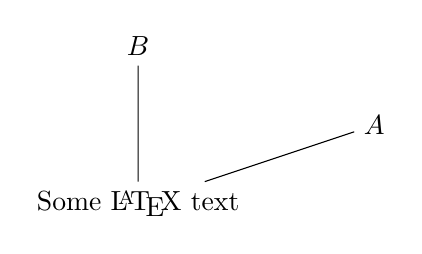
\begin{tikzpicture}
  \node (text) at (0,0) {%
    Some \LaTeX{} text};
  \node (A) at (3, 1) {\(A\)};
  \node (B) at (0, 2) {\(B\)};
  \draw (A) -- (text) -- (B);
\end{tikzpicture}
\end{example}
\TikZ{} attempts to be smart about the way it positions lines between nodes.
If you want to influence this, you can specify the exact connection-point on a node
after a dot. The available points are, for example, \cargv{north},
\cargv{west}, \cargv{south east} and so on. You can also put a number, which
will be interpreted as an angle (in degrees).
\begin{example}
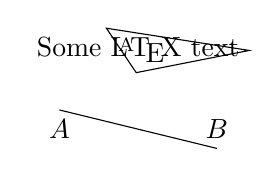
\begin{tikzpicture}
  \node (T) at (1,1) {%
    Some \LaTeX{} text};
  \node (A) at (0, 0) {\(A\)};
  \node (B) at (2, 0) {\(B\)};
  \draw (A.north) -- (B.south);
  \draw (T.0) -- (T.145)
    -- (T.265) -- cycle;
\end{tikzpicture}
\end{example}

Nodes can be created within paths by typing \ltx{node}
after a given coordinate or line. A node added after a line
is placed at its midpoint.
\begin{example}
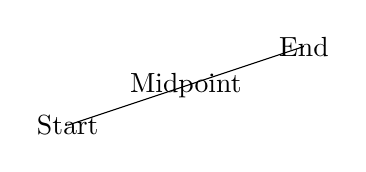
\begin{tikzpicture}
  \draw (0, 0) node {Start}
    -- node {Midpoint}
    (3, 1) node {End};
\end{tikzpicture}
\end{example}

If you want to create an empty node for the purpose of naming a specific point,
it is better to use the \csi{coordinate} command. This
ensures that the node is actually empty, whereas nodes created by \csi{node}
take up some space by default, even when they have no content.
\begin{example}
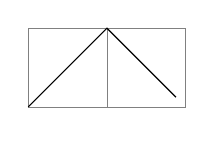
\begin{tikzpicture}
  \draw [help lines] (0, 0) grid (2, 1); % !hide
  \coordinate (A) at (0, 0);
  \coordinate (B) at (1, 1);
  \node (C) at (2, 0) {};
  \draw (A) -- (B) -- (C);
\end{tikzpicture}
\end{example}

\section{Curves and Shapes}

So far we have always used \ltx|--| to connect points. However,
this is not the only way. For example, if you wanted to only use horizontal and
vertical lines, you could specify \ltx/-|/ or \ltx/|-/ (according to preferred
order) as the connection between points.
\begin{example}
\tikz{\draw (0, 0) |- (2, 1);}
\tikz{\draw (0, 0) -| (2, 1);}
\end{example}

If you want to create curved lines, the simplest way is to use \ltx{to}
between points. It works the same as \ltx{--}, but you can provide an optional
argument, with \cargv{in} and \cargv{out} keys, to define the terminal angles of
the connection.
\begin{example}[vertical_mode, examplewidth=0.8\linewidth]
\tikzset{baseline} \vspace{-0.3cm} %!hide
\tikz{\draw (0, 0) to[out=90, in=-90] (2, 0);}
\tikz{\draw (0, 0) to[out=45] (2, 0);}
\vspace{-0.5cm} %!hide
\end{example}
The \cargv{looseness} key may be used to define how much the curve is
outstretched.
\begin{example}[vertical_mode, examplewidth=0.8\linewidth]
\tikzset{baseline} \vspace{-1cm} %!hide
\tikz{\draw (0, 0)
  to[out=90, in=-90, looseness=0.5] (2, 0);}
\tikz{\draw (0, 0)
  to[out=90, in=-90, looseness=2] (2, 0);}
\vspace{-1cm} %!hide
\end{example}
Often it might be easier to specify relative angles, using the \cargv{bend
  left} and \cargv{bend right} keys. If no angle is provided, a default value is
used.
\begin{example}[vertical_mode, examplewidth=0.8\linewidth]
\tikz{\draw (0, 0) to[bend left] (2, 0);}
\tikz{\draw (0, 0) to[bend right=90] (2, 0);}
\end{example}

If you need even finer control over the curves you, can use a
\ltx{.. controls ..} connection to specify a Bézier curve with one
or two control points.
\begin{chktexignore}
\begin{example}[vertical_mode, examplewidth=0.8\linewidth]
\vspace{-0.5cm} %!hide
\tikz{\draw (0, 0) .. controls (1, 1) .. (2, 0);}
\tikz{\draw (0, 0) .. controls (.5, 2) and (3, 1)
  .. (2, 0);}
\end{example}
\end{chktexignore}

In addition to curves, the points may also be connected using various shapes.
For example, the \ltx{grid} draws a grid between the points, while
\ltx{rectangle} draws a rectangle.
\begin{example}[vertical_mode, examplewidth=0.8\linewidth]
\tikz{\draw (0, 0) grid (2, 2);}
\tikz{\draw (0, 0) rectangle (3, 1);}
\end{example}
To specify how fine the grid is, use the \cargv{step} key.
\begin{example}[vertical_mode, examplewidth=0.8\linewidth]
\tikz{\draw (0, 0) grid[step=0.5] (2, 2);}
\tikz{\draw (0, 0) grid[step=1.5] (2, 2);}
\end{example}

Other shapes may also be drawn this way, sometimes requiring a specific syntax.
For example the \ltx{circle} interprets the left coordinate as its centre and
receives its radius via the \cargv{radius} key. You can also specify \cargv{x
  radius} and \cargv{y radius} separately, thus drawing an ellipse.\footnote{The
  \cargv{ellipse} shape can also be used in the same way if the naming irks you
  \smiley.}
\begin{example}[vertical_mode, examplewidth=0.9\linewidth]
\tikz{\draw (0, 0) circle[radius=1];}
\tikz{\draw (0, 0) circle[x radius=2, y radius=0.5];}
\end{example}
Many more shapes are available, such as \ltx{arc}, \ltx{parabola} or \ltx{sin}.
Be sure to check out the documentation\cite{pack:pgf} for the specifics of their use.

\section{Customizing Paths and Nodes}

By default, all paths are drawn with a continuous black line. You can modify
them by passing options to the \csi{draw} command. For example, passing
a colour name will change the colour of the line.
\begin{example}
\tikz{\draw[red]
  (0, 0) -- (1, 1);}
\tikz{\draw[blue]
  (0, 0) -- (1, 1);}
\end{example}

The thickness of a line can be controlled by passing the \cargv{line width} key
(specified in points by default), or by using one of the predefined values, such
as \cargv{semithick}, \cargv{very thin} or \cargv{ultra thick}.
\begin{example}
\tikz{\draw[line width=2]
  (0, 0) -- (1, 1);}
\tikz{\draw[very thin]
  (0, 0) -- (1, 1);}
\end{example}

The endings of lines can also be customized. For
example, \cargv{line cap} allows you to specify rounded
end-caps.
\begin{example}
\tikz{\draw[line width=10]
  (0, 0) -- (1, 1);}
\tikz{\draw[line width=10,
  line cap=round]
  (0, 0) -- (1, 1);}
\end{example}
You can turn a line into an arrow by specifying the \cargv{arrows} key.
\begin{example}
\tikz{\draw[arrows=->]
  (0, 0) -- (1, 1);}
\tikz{\draw[arrows=<<->]
  (0, 0) -- (1, 1);}
\end{example}

Lines do not need to be continuous, either. You can specify a \cargv{dash
  pattern} or use one of the predefined patterns.
\begin{example}
\tikz{\draw[dash pattern=
  on 4 off 1 on 2 off 1]
  (0, 0) -- (1, 1);}
\tikz{\draw[dotted]
  (0, 0) -- (1, 1);}
\end{example}

Adjust how lines are connected by using
\cargv{line join}. Set it to \cargv{round}, \cargv{bevel}, or
\cargv{miter}.
\begin{example}
\tikzset{every picture/.style={line width=6pt}} %!hide
\tikz{\draw[line join=round]
  (0, 0) -- (0.5, 1) -- (1, 0);}
\tikz{\draw[line join=bevel]
  (0, 0) -- (0.5, 1) -- (1, 0);}
\end{example}
If you want the line joins to be rounded, you can also pass the \cargv{rounded
  corners} key with the value set to the radius of the arc.
\begin{example}
\tikz{\draw[rounded corners]
  (0, 0) -- (0.5, 1) -- (1, 0);}
\tikz{\draw[rounded corners=25]
  (0, 0) -- (0.5, 1) -- (1, 0);}
\end{example}

Now, let's turn our attention to nodes. By default, a node's boundary is not
drawn, but you can pass \cargv{draw} and \cargv{fill}, optionally set to a
colour, to reveal it.
\begin{example}
\tikz{\node[draw] (0, 0)
  {Some Text};}
\tikz{\node[fill=red] (0, 0)
  {Some Text};}
\end{example}
By default, all nodes are rectangles, but they can be changed to circles by
passing the \cargv{circle} key to their options.
\begin{example}
\tikz{\node[draw, circle]
  (0, 0) {Some text};}
\end{example}

If you want to place multi-line text inside a node, you have to specify the
\cargv{align} key; without it, new lines are ignored. Possible values
are \cargv{left}, \cargv{center} and \cargv{right}.
\begin{example}
\tikz{\node[draw, align=left]
  (0, 0) {Some more\\ text};}
\tikz{\node[draw, align=center]
  (0, 0) {Even more \\ text};}
\end{example}

When nodes are placed along a path, their positions may be adjusted using the
\cargv{anchor} key. Its value is the point on the node boundary that should be
anchored on the given point in path.
\begin{example}
\tikz{\draw
  (0, 0) node[anchor=south] {A}
  -- node[anchor=north west] {B}
  (1, 1) node[anchor=135] {C};
}
\end{example}
Using relative commands, such as \cargv{left} or \cargv{above right}, for this
purpose usually leads to more readable code, though they are not so powerful.
\begin{example}
\tikz{\draw
  (0, 0) node[above] {A}
  -- node[below right] {B}
  (1, 1) node[right] {C};
}
\end{example}

All these options can be freely combined, but the resulting style specification
may turn out to be lengthy. To avoid retyping it for many nodes or paths, you
can define new styles. Some predefined styles already exist. For example, the
\cargv{help lines} style sets the colour of the lines to grey and makes them a bit
thinner, which is useful for drawing alignment grids when constructing your own
pictures.
\begin{example}
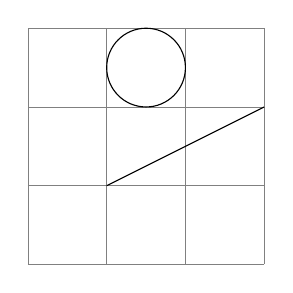
\begin{tikzpicture}
  \draw[help lines]
    (0, 0) grid (3,3);
  \draw (1, 1) -- (3,2);
  \draw (1.5, 2.5)
    circle[radius=0.5];
\end{tikzpicture}
\end{example}
To define your own style, pass a key of the form
\cargv{\carg{name}/.style=\carg{options}} to the \TikZ{} environment or
command options.
\begin{example}[vertical_mode, examplewidth=0.7\linewidth]
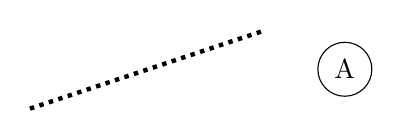
\begin{tikzpicture}[
  my line/.style={dotted, ultra thick},
  my node/.style={draw, circle},
]
  \draw[my line] (0, 0) -- (3, 1);
  \node[my node] at (4, 0.5) {A};
\end{tikzpicture}
\end{example}
If you want to set up some styles globally, you can also use the \csi{tikzset}
command.
\begin{example}
\tikzset{
  red style/.style={draw=red},
}
\tikz{\draw[red style]
  (0, 0) -- (1, 1) -- (2, 0);}
\tikz{\node[red style]
  at (0, 0) {Red node};}
\end{example}
If you want to avoid specifying the style for every node or path within a
\TikZ{} picture, you can set the special styles \cargv{every node} and
\cargv{every path} to change them all at once.
\begin{example}
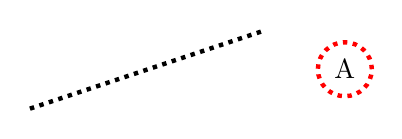
\begin{tikzpicture}[
  every path/.style={
    ultra thick, dotted},
  every node/.style={
    circle, draw=red},
]
  \draw (0, 0) -- (3, 1);
  \node at (4, 0.5) {A};
\end{tikzpicture}
\end{example}

\section{Coordinates}

So far, we have always used the default unit of centimetres for specifying
coordinates. However, it is possible to use any \LaTeX{} dimension (see
\autoref{sec:dimensions} for details).
\begin{example}
\tikz{\draw (0, 0)
  -- (1in, 1pt);}
\tikz{\draw (0, 0)
  -- (1dd, 1em);}
\end{example}

It is also possible to rescale how the distances are measured by using the
\cargv{scale} key. This is useful if you find that your picture is too big or
too small after drawing it, or if there exists some intuitive coordinate system
(for example, when drawing function plots).
\begin{example}
\tikz[scale=2]{\draw
  (0, 0) -- (1, 1);}
\tikz{\draw (0, 0) -- (2, 2);}
\end{example}
You can also specify \cargv{xscale} and \cargv{yscale} separately.

When specifying scale, you can use simple arithmetic operations. For example, to
change the dimensionless values to inches, you can pass \ltx{scale=1in/1cm}.
\begin{example}
\tikz[scale=1in/1cm]{\draw
  (0, 0) -- (1, 0.5);}
\tikz[scale=1em/1cm]{\draw
  (0, 0) -- (1, 0.5);}
\end{example}
Keep in mind that coordinates with dimensions will also be scaled, which may
have unintended consequences. A more robust way of changing dimensionless
values is the \cargv{x} and \cargv{y} keys.
\begin{example}
\tikz[x=1in, y=1in]{\draw
  (0, 0) -- (1, 0.5);}
\tikz[x=1em, y=10ex]{\draw
  (0, 0) -- (1, 0.5);}
\end{example}

You can actually specify three-dimensional coordinates when drawing pictures.
By default, the third coordinate is interpreted as a vector pointing \(45\)
degrees to the bottom left and is a bit shorter.\footnote{Formally,
  \((0, 0, 1)\) is  the same as \((-0.385, -0.385)\).}
This gives the effect of a parallel (or axonometric) projection.
\begin{example}[vertical_mode, examplewidth=0.85\linewidth]
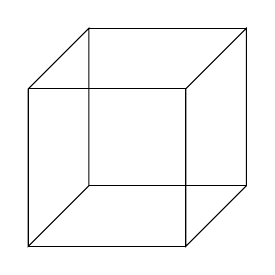
\begin{tikzpicture}[scale=2]
  \draw (0, 0, 0) -- (0, 0, 1) -- (0, 1, 1) --
    (0, 1, 0) -- cycle;
  \draw (1, 0, 0) -- (1, 0, 1) -- (1, 1, 1) --
    (1, 1, 0) -- cycle;
  \draw (0, 0, 0) -- (1, 0, 0) (0, 0, 1) -- (1, 0, 1)
    (0, 1, 1) -- (1, 1, 1) (1, 1, 0) -- (0, 1, 0);
\end{tikzpicture}
\end{example}
Length and direction can be changed by using the \cargv{z} key.

Sometimes, it may be easier to specify a path by using coordinates relative to
the previous point instead of absolute ones. To do so, prepend \ltx{++} to the
coordinate, which will be interpreted as the previous specified point plus
this vector.
\begin{example}
\begin{tikzpicture}[scale=2]
  \draw (0, 0) -- ++(0, 1) --
    ++(1, 0) -- ++(0, -1) --
    cycle;
  \draw (1.5, 0) -- ++(0, 1) --
    ++(1, 0) -- ++(0, -1) --
    cycle;
\end{tikzpicture}
\end{example}

Scaling is not the only transformation that can be applied to points. It is
also possible to rotate, shift, or apply an arbitrary linear transformation by
specifying its matrix. Check out the documentation for a detailed description.
\begin{example}
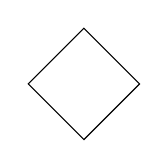
\begin{tikzpicture}[rotate=45]
  \draw (0, 0) -- (0, 1) --
    (1, 1) -- (1, 0) -- cycle;
\end{tikzpicture}
\end{example}
It is also possible to apply transformations to a single command.
\begin{example}
\begin{tikzpicture}
  \draw (0, 0) -- (1, 1);
  \draw[red, xshift=1cm]
    (0, 0) -- (1, 1);
\end{tikzpicture}
\end{example}
If you want to apply the same transformation to more than one command within
the same picture, you can use the \ei{scope} environment. It is especially useful
when your picture consists of more than one sub-picture, each of which is more
or less independent.
\begin{example}[vertical_mode, examplewidth=0.7\linewidth]
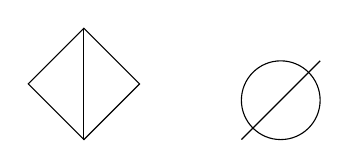
\begin{tikzpicture}
  \begin{scope}[rotate=45]
    \draw (0, 0) rectangle (1, 1);
    \draw (0, 0) -- (1, 1);
  \end{scope}
  \begin{scope}[xshift=2cm]
    \draw (0.5, 0.5) circle [radius=0.5];
    \draw (0, 0) -- (1, 1);
  \end{scope}
\end{tikzpicture}
\end{example}

When \TikZ{} pictures are positioned within text, their bottom end sits on the
baseline of the text. If you want to modify this, you can use the \cargv{baseline} key
to set the \(y\) coordinate at which the baseline should be. If no position is
specified, it defaults to \(0\).
\begin{example}[vertical_mode, examplewidth=0.8\linewidth]
text \tikz{\draw (0, 0) circle [radius=1em];}
text \tikz[baseline]{\draw
  (0, 0) circle [radius=1em];}
text \tikz[baseline=-0.5ex]{\draw
  (0, 0) circle [radius=1em];} text
\end{example}

\section{Reusing Pictures}

Sometimes, you may wish to draw the same picture at a few places within a bigger
one. While you could use the commands described in
\autoref{sec:simple_commands}, this would be problematic, since modifying their
placement or style is non-trivial. \TikZ{} comes with its own method of
defining smaller pictures, called `pics'. They can be created by passing
\cargv{\carg{name}/.pic=\carg{commands}} to the \TikZ{} environment or command,
and are then used by invoking the \csi{pic} command. An example is
presented in \autoref{lst:pics}.
\begin{listing}
  \begin{example}[vertical_mode, examplewidth=0.9\linewidth]
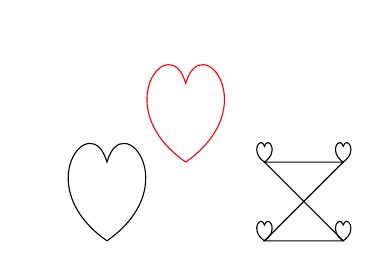
\begin{tikzpicture}[
  heart/.pic={
    \draw (0,0) .. controls (-1, 0.7) and (-0.2, 1.7)
    .. (0, 1) .. controls  (0.2, 1.7) and (1, 0.7)
    .. (0, 0);
  },
]
  \pic at (0, 0) {heart};
  \pic[red] at (1, 1) {heart};

  \begin{scope}[xshift=2cm, every pic/.style={scale=0.2}]
    \draw (0, 0) pic {heart} -- (1, 1) pic {heart} --
      (0, 1) pic {heart} -- (1, 0) pic {heart} -- cycle;
  \end{scope}
\end{tikzpicture}
\end{example}
  \caption{An example of using pics in \TikZ{}.}\label{lst:pics}
\end{listing}

If you find yourself repeating a lot of simple commands (for example, drawing
ticks on an axis), you may simplify your code by using the \csi{foreach} command. It
repeats the drawing command for each value in a list, so that you can
write repeatable code once, and need only modify the important parts.
\begin{example}[vertical_mode, examplewidth=0.8\linewidth]
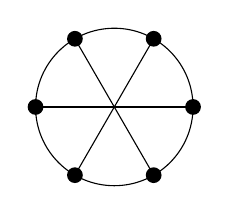
\begin{tikzpicture}
  \draw (0, 0) circle[radius=1cm];
  \foreach \i in {0, 60, 120, 180, 240, 300} {
    \draw (0, 0) -- (\i: 1);
    \fill (\i: 1) circle[radius=0.1cm];
  }
\end{tikzpicture}
\end{example}
If your values are a simple arithmetic sequence, you need only provide the first
two values and the last, replacing the rest with triple dots.
\begin{example}[vertical_mode, examplewidth=0.8\linewidth]
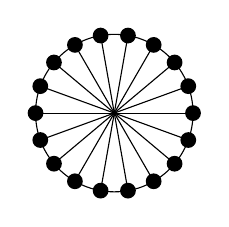
\begin{tikzpicture}
  \draw (0, 0) circle[radius=1cm];
  \foreach \i in {0, 20, ..., 340} {
    \draw (0, 0) -- (\i: 1);
    \fill (\i: 1) circle[radius=0.1cm];
  }
\end{tikzpicture}
\end{example}
You can also iterate over pairs by separating respective parts with \ltx{/}.
\begin{example}
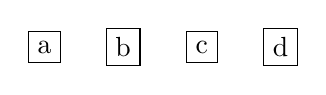
\begin{tikzpicture}
  \foreach \i/\j in {0/a,
    1/b, 2/c, 3/d} {
    \node[draw] at (\i, 0) {\j};
  }
\end{tikzpicture}
\end{example}

\section{Libraries}

\pai{pgf} and \TikZ{} do not rely on \LaTeX{}. In fact, they can be used with
any \TeX{} based system or even \TeX{} itself. For this reason, \TikZ{}
provides its own system of extensions that does not use \LaTeX{}'s
\cs{usepackage} command. Extensions of \TikZ{} are called libraries, and can be
loaded using the \csi{usetikzlibrary} command, which receives a list of comma
separated libraries.

For example, if you intend to draw some geometry problems, you will often find
yourself looking for intersections of objects. While you could calculate
their exact coordinates by hand, the \cargv{intersections} library will do it
for you. An example is presented in \autoref{lst:intersections}.

\begin{listing}
  \begin{example}[vertical_mode, examplewidth=0.8\linewidth]
%!showbegin !hide
% In preamble
\usetikzlibrary{intersections}
% ...
%!showend !hide

\begin{tikzpicture}
  \draw[name path=O] (0, 0) circle [radius=1];
  \draw[name path=L] (-2, -1.5) -- (3, 1);

  \fill[red, name intersections={of=O and L}]
    (intersection-1) circle[radius=2pt]
    (intersection-2) circle[radius=2pt];
\end{tikzpicture}
\end{example}
  \caption{An example of using \cargv{intersections}
    library.}\label{lst:intersections}
\end{listing}

Other libraries extend the number of available shapes. For example, the
\cargv{arrows.meta} library defines numerous additional arrow tips, if you do
not like the classical one. Some are presented in
\autoref{lst:arrows.meta}.

\begin{listing}
  \begin{example}[vertical_mode, examplewidth=0.8\linewidth]
%!showbegin !hide
% In preamble
\usetikzlibrary{arrows.meta}
% ...
%!showend !hide

\tikzset{every path/.style={ultra thick}} %!hide2
\tikz{\draw[->] (0, 0) -- (1, 1);}
\tikz{\draw[-{Circle}] (0, 0) -- (1, 1);}
\tikz{\draw[-{Stealth}] (0, 0) -- (1, 1);}
\tikz{\draw[-{Stealth[round]}] (0, 0) -- (1, 1);}
\tikz{\draw[-{Diamond[open]}] (0, 0) -- (1, 1);}
\end{example}
  \caption{Some of the arrow tips defined by \cargv{arrows.meta}
    library.}\label{lst:arrows.meta}
\end{listing}

You can perform additional calculations on existing
coordinates. The \cargv{calc} library allows you to do so by enclosing them
within \verb|$| symbols. An example is presented in
\autoref{lst:calc}.

\begin{listing}
  \begin{example}[vertical_mode, examplewidth=0.8\linewidth]
%!showbegin !hide
% In preamble
\usetikzlibrary{calc}
% ...
%!showend !hide

\begin{tikzpicture}
  \coordinate (A) at (1, -1);
  \coordinate (B) at (0, 1);
  \draw[red, ->] (0, 0) -- node[above] {\(A\)} (A);
  \draw[blue, ->] (0, 0) -- node[left] {\(B\)} (B);
  \draw[green, ->] (0, 0) --
      node[below right] {\(A+2B\)} ($(A)+2*(B)$);
\end{tikzpicture}
\end{example}
  \caption{An example of using the \cargv{calc} library.}\label{lst:calc}
\end{listing}

If you have a lot of \TikZ{} code in your document, you may notice that
compiling it takes much longer. This is because
\TikZ{} redraws each picture with every \LaTeX{} pass. If this becomes
annoying, you can cache your images to external files and reuse them on
subsequent runs. To do this, simply put the following code in your preamble.
\begin{minted}{latex}
\usetikzlibrary{external}
\tikzexternalize
\end{minted}
This method has some limitations, but should be sufficient for most uses. Read
up on it in the documentation if problems occur.

These are not the only libraries---additional node shapes, real 3D-perspective,
matrices, mind maps and many more are covered. Most of them are described in
the \pai*{pgf} package documentation. Check it out if you haven't found
solution to your problem here.


% The Not So Short Introduction to LaTeX
%
% Copyright (C) 1995--2022 Tobias Oetiker, Marcin Serwin, Hubert Partl,
% Irene Hyna, Elisabeth Schlegl and Contributors.
%
% This document is free software: you can redistribute it and/or modify it
% under the terms of the GNU General Public License as published by the Free
% Software Foundation, either version 3 of the License, or (at your option) any
% later version.
%
% This document is distributed in the hope that it will be useful, but WITHOUT
% ANY WARRANTY; without even the implied warranty of MERCHANTABILITY or FITNESS
% FOR A PARTICULAR PURPOSE.  See the GNU General Public License for more
% details.
%
% You should have received a copy of the GNU General Public License along with
% this document.  If not, see <https://www.gnu.org/licenses/>.

% !TEX root = ./lshort.tex
%%%%%%%%%%%%%%%%%%%%%%%%%%%%%%%%%%%%%%%%%%%%%%%%%%%%%%%%%%%%%%%%%
% Contents: Customising LaTeX output
% $Id$
%%%%%%%%%%%%%%%%%%%%%%%%%%%%%%%%%%%%%%%%%%%%%%%%%%%%%%%%%%%%%%%%%
\chapter{Customising \LaTeX}\label{chap:custom}

\begin{intro}
  Documents produced with the commands you have learned up to this
  point will look acceptable to a large audience. While they are not
  fancy-looking, they obey all the established rules of good
  typesetting, which will make them easy to read and pleasant to look at.

  However, there are situations where \LaTeX{} does not provide a
  command or environment that matches your needs, or the output
  produced by some existing command may not meet your requirements.

  In this chapter, I will try to give some hints on
  how to teach \LaTeX{} new tricks and how to make it produce output
  that looks different from what is provided by default.
\end{intro}

\section{New Commands, Environments and Packages}

At the beginning of this book we have mentioned that \LaTeX{} allows us to
write documents using logical markup, with commands like \csi{emph} or \csi{section}. There
may be however situations where \LaTeX{} does not provide an appropriate command for the content you want to write about.
You may have noticed that all the
commands I introduce in this book are typeset in a box, and that they show up
in the index at the end of the book. There is no \LaTeX{} markup to format example code or commands, but \LaTeX{} allows me to define my own commands for this purpose. I
can write:

\begin{example}
\begin{lscommand}
  \csi{dum}
\end{lscommand}
\end{example}

In this example, I am using both a new environment called
\ei{lscommand}, which is responsible for drawing the box around the
command, and a new command named \csi{csi}, which typesets the command
name and makes a corresponding entry in the index. Check
this out by looking up the \csi{dum} command in the index at the back
of this book, where you'll find an entry for \csi{dum}, pointing to
every page where I mentioned the \csi{dum} command.

If I ever decide that I do not like having the commands typeset in
a box any more, I can simply change the definition of the
\ei{lscommand} environment to create a new look. This is much
easier than going through the whole document to hunt down all the
places where I have used some generic \LaTeX{} commands to draw a
box around some word.

\subsection{New Commands}\label{sec:new_commands}

You have already learned some basic command creation in
\autoref{sec:simple_commands}. The main command is the
\begin{lscommand}
  \csi{NewDocumentCommand}[name:M, argspec:m, definition:m]
\end{lscommand}
It requires three arguments: the \carg{name} of the command you want to create,
the \carg{argspec} (argument specification) and the \emph{definition} of the
command.

The \carg{argspec} argument specifies the number and types of arguments the
command receives. The two most important types are \cargv{m}, for
\emph{mandatory} and \cargv{o} for \emph{optional}. To create a command that
takes two optional arguments, then two mandatory, then again one optional and
finally three mandatory you would write \cargv{oommommm}. If the \carg{argspec}
argument is empty then the command will take no arguments, as you have already
seen.

This example defines a new command called \csi{tnss}. This is
short for \enquote{The Not So Short Introduction to \LaTeX}. Such a command
could come in handy if you had to write the title of this book over
and over again.

\begin{example}
\NewDocumentCommand{\tnss}{}{%
  The not so Short Introduction
    to \LaTeX}
This is \enquote{\tnss} \ldots{}
\enquote{\tnss}
\end{example}

The next example illustrates how to define a new command that takes two
arguments. In order to refer to the received arguments you use
\mintinline{latex}|#1| for the first argument, \mintinline{latex}|#2| for the
second, and so on.

\begin{example}
\NewDocumentCommand{\txsit}{mm}
 {This is the \emph{#1}
  #2 Introduction to \LaTeX}

% in the document body:
\txsit{not so}{short}

\txsit{very}{long}
\end{example}

If your command accepts an optional argument, but the user does not supply one,
a special marker \cargv{-NoValue-} will be inserted instead.
\begin{example}
\NewDocumentCommand{\txsit}{om}
{This is the \emph{#1}
  #2 Introduction to \LaTeX}

% in the document body:
\txsit{definitive}

\txsit[very]{long}
\end{example}
In order to test whether the user supplied a value, use
\begin{lscommand}
  \csi{IfValueTF}[argument:m, value version:m, no value version:m]
\end{lscommand}
macro.
\begin{example}
\NewDocumentCommand{\MyCommand}{o}{
  \IfValueTF {#1} {
    Optional argument: #1.
  } {
    No optional argument given.
  }%
}

\MyCommand\\
\MyCommand[hello]
\end{example}

There are two variations of it: \csi{IfValueT} and \csi{IfValueF} which may
be used if you only need output for one of the branches. The example with
\cargv{-NoValue-} in the output could be fixed by writing
\begin{example}
\NewDocumentCommand{\txsit}{om}
{This is the
  \IfValueT{#1}{\emph{#1} }%
  #2 Introduction to \LaTeX}

% in the document body:
\txsit{definitive}

\txsit[very]{long}
\end{example}
The commands \csi{IfNoValueTF}, \csi{IfNoValueT} and \csi{IfNoValueF}
work exactly the same, but the value\slash{}no-value branches are swapped.

Often you will want to use optional arguments when present but use some default
values when the user does not provide them. This could be achieved by
\csi{IfValueTF}, but with the \cargv{O} argument a default value can be set directly.
It works like \cargv{o} but allows setting a default
if no value is supplied. Write

\begin{example}
\NewDocumentCommand{\txsit}{O{not so}m}
{This is the \emph{#1}
  #2 Introduction to \LaTeX}

% in the document body:
\txsit{definitive}

\txsit[very]{long}
\end{example}

Another useful argument specification is \cargv{s}, short for star. This
argument allows providing different definitions based on whether the
starred or non-starred version of command was issued by the user. It uses
\csi{IfBooleanTF} command (and its variations\csih{IfBooleanT}\csih{IfBooleanF})
that works like the \csi{IfValueTF} command.

\begin{chktexignore}
  \begin{example}
\NewDocumentCommand{\txsit}{sO{not so}m}
{This is the \emph{#2}
  #3 Introduction to \LaTeX%
  \IfBooleanT{#1}{%
    : Superstar Edition%
  }%
}

% in the document body:
\txsit{long}\\
\txsit*{long}
\end{example}
\end{chktexignore}

These are just the most common argument specifications. For a full description,
take a look at the~\cite{usrguide3}.

As we have discussed in \autoref{sec:simple_commands}, \LaTeX{} will not allow
you to create a new command that would overwrite an existing one, you can do so
using \csi{RenewDocumentCommand}. It uses the same argument specification
syntax as the \csi{NewDocumentCommand} command.

In some cases you might want to use the \csi{ProvideDocumentCommand} command.
It works like \csi{NewDocumentCommand}, but if the command is already defined,
\LaTeX{} will silently ignore the new definition. Yet another variant is the
\csi{DeclareDocumentCommand}. It always creates the given command, overwriting
old definition if it exists.

\subsection{New Environments}
The \csi{NewDocumentEnvironment} command lets you create your own environments. It has the
following syntax:

\begin{lscommand}
  \small
  \csi{NewDocumentEnvironment}[name:m, argspec:m, at begin:m, at end:m]
\end{lscommand}
The \carg{argspec} argument is the same as in the
\csi{NewDocumentCommand} command. The contents of \carg{at begin} and \carg{at
  end} arguments will be inserted respectively when the commands
\csi{begin}[name: m] and \csi{end}[name: m] is encountered. The example
presented in \autoref{lst:kingenv} illustrates the usage of this command.
\begin{listing}
  \begin{example}
\NewDocumentEnvironment{king}{}{%
  \emph{Listen! For the
    king made a statement:}%
  \\[1em]%
} {%
  \\[1em]%
  \emph{This concludes
    the king's statement.}%
}

\begin{king}
My humble subjects \ldots
\end{king}
\end{example}
  \caption{An example of using \csi{NewDocumentEnvironment}
    command.}\label{lst:kingenv}
\end{listing}

Note that when environment argument are read, they are read \emph{after} the
\csi{begin}[name: m] command. This may be especially counterintuitive when we
consider the \cargv{s} specification. \autoref{lst:kingsenv} illustrates this.
\begin{listing}
  \begin{example}
\NewDocumentEnvironment{king}{s}{%
  \IfBooleanTF{#1}{
    \begin{center}
      \emph{Thus spoke Charles I:}
      \\[1em]%
    \end{center}%
  } {
    \emph{Listen! For the
      king made a statement:}%
      \\[1em]%
  }%
} {%
  \\[1em]%
  \emph{This concludes
    the king's statement.}%
}

\begin{king}*
My humble subjects \ldots
\end{king}
\end{example}
  \caption{An example of using the \cargv{s} specifier when defining a new
    environment.}\label{lst:kingsenv}
\end{listing}
If you want to create a starred version of an environment (similar to the
\hologo{AmSLaTeX} environments) you have to define it separately.
\begin{minted}{latex}
\NewDocumentEnvironment{king}{moo} { ... } { ... }
\NewDocumentEnvironment{king*}{moo} { ... } { ... }
\end{minted}
Obviously you can use the same internal commands to define them, for example
renaming the previous implementation to \cargv{kinginternal} making the
\cargv{king} and \cargv{king*} a thin wrapper around it.

The \csi{NewDocumentEnvironment} also introduces a special argument
specification: \cargv{+b}, short for body.\footnote{The \cargv{+} indicates
  that it may contain multiple paragraphs.} It is only allowed as the last
argument in the \carg{argspec}. It allows you to receive the body of the
environment as an argument.
\begin{example}
\NewDocumentEnvironment{twice}{+b} {%
  First time:\\ #1

  Second time:\\ #1
} {}

\begin{twice}
This will be printed twice!
\end{twice}
\end{example}
While this makes one of the \carg{at begin}, \carg{at end} arguments redundant,
they are still required. (In the example above we provided an empty \carg{at
  end}.)

Do not overuse \cargv{+b} as this will both add limitations to the environments
like \csi{verb} not being allowed inside and it will slow down the
typesetting.

Similar to the \csi{NewDocumentCommand}, \LaTeX{} makes sure that you do not
define an environment that already exists. If you ever want to change an
existing environment, use the \csi{RenewDocumentEnvironment} command. Its
arguments are the same as the \csi{NewDocumentEnvironment} command.

\subsection{Copying commands}\label{sec:copyingcommands}

When redefining commands you may want to use the original version of the
command. Your initial code may look like this
\begin{minted}{latex}
\RenewDocumentCommand{\emph}{m}{%
  \emph{#1}~(\enquote{#1} is emphasised)%
}
\end{minted}
but when you try to compile the document you will get the error message
\begin{verbatim}
! TeX capacity exceeded, sorry [input stack size=5000].
\end{verbatim}

To understand why this happens it is instructive to consider how \TeX{} expands
the defined commands. The above \csi{RenewDocumentCommand} tells the \TeX{}
engine that whenever \csi{emph}[foo:vm] is seen it must replace it with
\mintinline{latex}|\emph{foo}~(\enquote{foo} is emphasised)|. You may already see the
problem here. In the next stage it will again replace the \csi{emph}[foo:vm]
yielding
\begin{minted}[breaklines]{latex}
\emph{foo}~(\enquote{foo} is emphasised)~(\enquote{foo} is emphasised)
\end{minted}
This process will never end and at some point \TeX{}
simply gives up.

Note that
\begin{minted}{latex}
\NewDocumentCommand{\oldemph}{m}{\emph{#1}}
\RenewDocumentCommand{\emph}{m}{%
  \oldemph{#1}~(\enquote{#1} is emphasised)%
}
\end{minted}
will suffer the same fate since \mintinline{latex}|\oldemph{...}| %chktex 11 
will  be replaced by \TeX{} with \mintinline{latex}|\emph{...}| and %chktex 11
the  cycle repeats.

In order to avoid this problem a special command exists
\begin{lscommand}
  \csi{NewCommandCopy}[name:M, command:M]
\end{lscommand}
It makes the \carg{name} the exact copy of the \carg{command}. The following example shows how this works
\begin{example}[examplewidth=0.35\linewidth]
\NewDocumentCommand{\foo}{}{Batman!}

\NewDocumentCommand{\newfoo}{}{\foo}
\NewCommandCopy{\copiedfoo}{\foo}

\RenewDocumentCommand{\foo}{}{Na Na Na}

\foo{} \newfoo{} \copiedfoo{}
\end{example}

This is precisely the behaviour we need in order to redefine the \csi{emph}
command as we have tried to do earlier.
\begin{example}[examplewidth=0.35\linewidth]
\NewCommandCopy{\oldemph}{\emph}
\RenewDocumentCommand{\emph}{m}{%
  \oldemph{#1}~(\enquote{#1}
  is emphasised)%
}

And here it \emph{comes}.
\end{example}

\subsection{Command-line \LaTeX}

If you work on a Unix-like OS, you might be using Makefiles to build your
\LaTeX{} projects. In that connection it might be interesting to produce
different versions of the same document by calling \LaTeX{} with command-line
parameters. If you add the following structure to your document:

\begin{minted}{latex}
\IfBooleanTF{\blackandwhite} {
  % "black and white" mode; do something...
} {
  % "color" mode; do something different...
}
\end{minted}

Now compile document like this:
\begin{verbatim}
xelatex '\NewCommandCopy{\blackandwhite}{\BooleanTrue}
    \input{test.tex}'
\end{verbatim}
First the command \verb|\blackandwhite| is defined as the \csi{BooleanTrue} macro which
holds a special value used in \csi{IfBooleanTF} checks. Then the actual file is
read with input. By setting \verb|\blackandwhite| to \csi{BooleanFalse} the
colour version of the document would be produced.

\subsection{Your Own Package}

If you define a lot of new environments and commands, the preamble of
your document will get quite long. In this situation, it is a good
idea to create a \LaTeX{} package containing all your command and
environment definitions. Use the \csi{usepackage}
command to make the package available in your document.

\begin{listing}
  \begin{lined}{\textwidth}
    \begin{minted}{latex}
\ProvidesExplPackage{demopack}{2022-05-05}{0.1}{%
  Package by Tobias Oetiker
}

\NewDocumentCommand{\tnss}{} {
  The~not~so~Short~Introduction~to~\LaTeX
}
\NewDocumentCommand{\txsit}{O{not~so}} {
  The~\emph{#1}~Short~Introduction~to~\LaTeX
}

\NewDocumentEnvironment{king}{} {
  \begin{quote}
} {
  \end{quote}
}
\end{minted}
  \end{lined}
  \caption{Example Package.}\label{package}
\end{listing}

Writing a package basically consists of copying the contents of your document
preamble (with minor adjustments) into a separate file with a name ending in
\texttt{.sty}. There is one special command,
\begin{lscommand}
  \csi{ProvidesExplPackage}[name:m, date:m, version:m, description:m]
\end{lscommand}
for use at the very beginning of your package file. This command tells the
\LaTeX{} to process the  file in \emph{expl mode}. The most visible effect of
this is that all whitespace is ignored. You may have noticed that in many of
the examples above we had to end most lines with \ai{\%} to get correct spacing
in the output. In \emph{expl mode}, spaces have to be added explicitly if
needed at all. They are usually quite rare when writing a package. To insert
spaces, use the \ai{\~} character, which normally denotes non-breaking
space.\footnote{If you want to insert non-breaking space in \emph{expl mode},
  use \csi{nobreakspace}.} Paragraphs can be started with the \csi{par} command.

The arguments are used to provide information about package in the log file. If
you use this package and look at the log file you will find
\begin{verbatim}
Package: demopack 2022-05-05 v0.1 Package by Tobias Oetiker
\end{verbatim}
in the \eei{.log} file.

\csi{ProvidesExplPackage} will also issue a sensible error message when you try
to include a package twice. \autoref{package} shows a small example package
that contains the commands defined in the examples above.

\section{Fonts and Sizes}\label{sec:fontsize}

\subsection{Font Changing Commands}\index{font}\index{font size}

\LaTeX{} fonts are influenced by four parameters
\begin{description}
  \item[family] The collection of fonts. For example, \enquote*{Latin Modern
      Roman} or \enquote*{Source Code Pro}.
  \item[series] The weight of the font. For example, \enquote*{bold} or
    \enquote*{medium}.
  \item[shape] The shape of glyphs within a font family. For example,
    \enquote*{small caps} or \enquote*{italics}.
  \item[size] The size of the glyphs. For example, \enquote*{\qty{10}{pt}} or
    \enquote*{\qty{12}{pt}}.
\end{description}
\LaTeX{} automatically chooses the appropriate font family, series, shape and
size based on the logical structure of the document (sections, footnotes,
emphasis, \ldots). It is possible however to instruct \LaTeX{} manually which
font to use. It is important to note that not every combination of
family\slash{}series\slash{}shape exists as an actual font. \LaTeX{} will
complain if you try for something that does not exist.

\LaTeX{} predefines three font families to use throughout the document: the
upright or roman family accessible via \csi{textrm}, the \textsf{sans serif
  family} accessible via \csi{textsf} and monospace or typewriter family
accessible via \csi{texttt}.
\begin{example}
\textrm{Roman is the default
  in articles.} \\
\textsf{Sans serif is used in
  presentations.} \\
\texttt{Monospace is used in
  verbatim code blocks.}
\end{example}

There are only two predefined \LaTeX{} series: medium (\csi{textmd}) and bold
(\csi{textbf}).
\begin{example}
\textmd{The default.} \\
\textbf{Bold font.}
\end{example}

Shapes are a bit more complicated. The three basic shapes are: italics
(\csi{textit}), oblique or slanted\footnote{Oblique shape differs from the
  italics in that italic shape uses different glyphs while oblique shape uses
  the same glyphs but slanted. The difference is really obvious
  \fontspec{cmunui.otf} when you look at the unslanted italic
  font.} (\csi{textsl}) and small capitals (\csi{textsc}).
\begin{example}
\textit{Italic shape.} \\
\textsl{Slanted shape.} \\
\textsc{Small Capitals.}
\end{example}
However there are two additional shapes that are not provided by default
\LaTeX{} fonts: swash (\csi{textsw}), for decorative fonts and spaced caps and
small caps (\csi{textssc}). These are rarely used but may come in handy when
using custom fonts as described in \autoref{sec:fontspec}.
\begin{example}
\setmainfont{EB Garamond} %!hide
Question vs. \textsw{Question}
\end{example}
In addition two virtual shapes are provided: upright (\csi{textup}) and
upper-lowercase (\csi{textulc}). These are not actually shapes but utility
commands. The former one switches back to upright font while the latter
disables small capitals. The command \csi{textnormal} is just the combination
of the two.
\begin{example}
\textsl{\textsc{Back to
  \textup{upright.}}} \\
\textsl{\textsc{Back to
  \textulc{lowercase.}}} \\
\textsl{\textsc{Back to
  \textnormal{normal.}}}
\end{example}

All of the commands described above also exist in their switch version. Instead
of receiving the text via argument, they change the font permanently until it is
changed again. For example, the switch version of \csi{textit} and \csi{textrm}
are \csi{itshape} and \csi{rmfamily}, respectively. While the argument versions
are useful for defining commands, switch versions are especially useful when
defining your own environments.
\begin{example}
Only \textit{argument} is
affected. After \itshape
everything is in italics
until \upshape is encountered.
\end{example}
Both argument and switch versions of the described commands are presented in
\autoref{tbl:fonts}.
\begin{table}
  \caption{Default font changing commands of \LaTeX.}\label{tbl:fonts}
  \begin{tabular}{@{}lll@{}}
    \toprule
    Argument Command         & Switch           & Example                      \\
    \midrule
    \csi{textrm}[text:m]     & \csi{rmfamily}   & \textrm{\wi{roman}}          \\
    \csi{textsf}[text:m]     & \csi{sffamily}   & \textsf{\wi{sans serif}}     \\
    \csi{texttt}[text:m]     & \csi{ttfamily}   & \texttt{typewriter}          \\[6pt]
    \csi{textmd}[text:m]     & \csi{mdseries}   & \textmd{medium}              \\
    \csi{textbf}[text:m]     & \csi{bfseries}   & \textbf{\wi{bold face}}      \\[6pt]
    \csi{textup}[text:m]     & \csi{upshape}    & \textup{\wi{upright}}        \\
    \csi{textit}[text:m]     & \csi{itshape}    & \textit{\wi{italic}}         \\
    \csi{textsl}[text:m]     & \csi{slshape}    & \textsl{\wi{slanted}}        \\
    \csi{textsc}[text:m]     & \csi{scshape}    & \textsc{\wi{Small Caps}}     \\
    \csi{textsw}[text:m]     & \csi{swshape}    & \textsw{\wi{Queen of Swash}} \\[6pt]
    \csi{textnormal}[text:m] & \csi{normalfont} & \textnormal{document} font   \\
    \bottomrule
  \end{tabular}
\end{table}

When working with switch versions of fonts that are slanted right it is
important to remember about \wi{italic correction}. This is a small space after
the end of right slanting text that is sometimes necessary to avoid overlapping
letters. It is inserted using \csi{/} command.
\begin{chktexignore}  
\begin{example}
Without: {\itshape oof}bar \\
With: {\itshape oof\/}bar
\end{example}
\end{chktexignore}
The italic correction is handled automatically by the argument versions of the
commands.

In contrast to the previous font changing commands, the size of font can only
be controlled via switch versions. \LaTeX{} predefines some switches for
changing font size, see \autoref{sizes} and \autoref{tab:pointsizes} for their
description.
\begin{table}
  \caption{Commands changing font size.}\label{sizes}\index{font size}
  \begin{tabular}{@{}ll@{\qquad}ll@{}}
    \toprule
    Command                     & Size                             &
    Command                     & Size                               \\
    \midrule
    \csi{tiny}                  & \tiny tiny                       &
    \csi{Large}                 & \Large larger                      \\
    \csi{scriptsize}            & \scriptsize very small           &
    \csi{LARGE}                 & \LARGE very large                  \\
    \csi{footnotesize}          & \footnotesize  quite small       &
    \multirow{2}{*}{\csi{huge}} & \multirow{2}{*}{\huge huge}        \\
    \csi{small}                 & \small small                     &
                                &                                    \\
    \csi{normalsize}            & \normalsize  normal              &
    \multirow{2}{*}{\csi{Huge}} & \multirow{2.2}{*}{\Huge largest}   \\
    \csi{large}                 & \large large                     &
                                &                                    \\
    \bottomrule
  \end{tabular}
\end{table}

\begin{table}
  \caption[Absolute point sizes in standard classes.]{Absolute point sizes in
    standard classes depending on the class option. The default class option is
    \cargv{10pt}.}\label{tab:pointsizes}\label{tab:sizes}
  \sisetup{table-format=2.2}
  \begin{tabular}{@{}lSSS@{}}
    \toprule
                       & \multicolumn{3}{c}{Size (\unit{pt})}                                   \\
    \cmidrule(l){2-4}
    Command            & {\cargv{10pt}}                       & {\cargv{11pt}} & {\cargv{12pt}} \\
    \midrule
    \csi{tiny}         & 5                                    & 6              & 6              \\
    \csi{scriptsize}   & 7                                    & 8              & 8              \\
    \csi{footnotesize} & 8                                    & 9              & 10             \\
    \csi{small}        & 9                                    & 10             & 10.95          \\
    \csi{normalsize}   & 10                                   & 10.95          & 12             \\
    \csi{large}        & 12                                   & 12             & 14.4           \\
    \csi{Large}        & 14.4                                 & 14.4           & 17.28          \\
    \csi{LARGE}        & 17.28                                & 17.28          & 20.74          \\
    \csi{huge}         & 20.74                                & 20.74          & 24.88          \\
    \csi{Huge}         & 24.88                                & 24.88          & 24.88          \\
    \bottomrule
  \end{tabular}
\end{table}

When using these commands it is important to remember that the
line spacing is only updated after the paragraph ends. To avoid putting empty
lines before the closing curly brace you may use the \csi{par} command.
\begin{example}
{\Large Here the line spacing
  is not updated. A bit tight!}

{\Large Much better! I can
  breathe freely again!\par}
\end{example}

An arbitrary font size can be specified using the
\begin{lscommand}
  \csi{fontsize}[size: m, line skip: m]\csi{selectfont}
\end{lscommand}
command combo. The \carg{line skip} determines the height of the text line and
should be usually around \(1.2\) times larger than the \carg{size}.
\begin{example}[vertical_mode, examplewidth=0.7\linewidth]
\fontsize{2cm}{2.4cm}\selectfont A big one!
\end{example}

Fun fact: \LaTeX{} default font is a bit unusual in that it looks slightly
different depending on its size. The difference is presented in the table below
where the text written using different sizes was rescaled to the same height.
\begin{center}
  \begin{tabular}{@{}lll@{}}
    \toprule
    \csi{tiny}                           &
    \csi{normalsize}                     &
    \csi{Huge}                             \\
    \midrule
    \resizebox{!}{2em}{\tiny Text}       &
    \resizebox{!}{2em}{\normalsize Text} &
    \resizebox{!}{2em}{\Huge Text}         \\
    \bottomrule
  \end{tabular}
\end{center}

If you need to access even more font variants and shapes\footnote{For example
  the aforementioned \fontspec{cmunui.otf} upright italic shape.} check out
\citetitle{fntguide}~\cite{fntguide}.

\subsection{Danger, Will Robinson, Danger}

Note! Using explicit font setting commands defies the basic idea of
\LaTeX{} described in \autoref{sec:logical_structure}, which is to separate the
logical and visual markup. The fonts should get switched automatically
according to the requirements of the context. A simple rule of thumb: If you
use the same font changing command in several places in order to typeset a
special kind of information, you should use \csi{NewDocumentCommand} to define
a \enquote{logical wrapper command} for the font changing command.

\begin{example}
\NewDocumentCommand{\oops}{m}{%
 \textbf{#1}}
Do not \oops{enter} this room,
it's occupied by \oops{machines}
of unknown origin and purpose.
\end{example}

This approach has the advantage that you can decide at some later
stage that you want to use a visual representation of danger other
than \csi{textbf}, without having to wade through your document,
identifying all the occurrences of \csi{textbf} and then figuring out
for each one whether it was used for pointing out danger or for some other
reason.

\subsection{Advice}

To conclude this journey into the land of fonts and font sizes,
here is a little word of advice:\nopagebreak

\begin{quote}
  \underline{\textbf{Reme\(\mathfrak{mber}\)\Huge!}} \textit{The}
  \textsf{M\textbf{\LARGE O} \(\mathcal{R}\)\textsl{E}} fonts \Huge you
  \tiny use \footnotesize \textbf{in} a \small \texttt{document},
  \large \textit{the} \normalsize more \textsc{readable} and
  \textsl{\textsf{beautiful} it bec\large o\Large m\LARGE e\huge s}.
\end{quote}

\section{Custom Fonts with \pai{fontspec}}\label{sec:fontspec}

In the following examples we use Adobe Source fonts~\cites{sourceserif,
  sourcesans, sourcecodepro}. These fonts are included with \TeXLive{} \LaTeX{}
distributions and should be available in the directory
\begin{code}
  \nolinkurl{.../texmf-dist/fonts/opentype/adobe}
\end{code}
where the \cargv{...} denotes the install-path of \TeXLive{}.
\hologo{LuaTeX} checks this directory automatically, so it should work fine,
but if you are using \hologo{XeTeX} you must first install these fonts in your
system. You can also download and install them manually from the links provided
in the bibliography. Alternatively swap out their respective names with some other
fonts installed in your system.

Many free OpenType fonts are available at \url{https://fontlibrary.org/}.

\subsection{Main Document Fonts}

If you are not pleased with the default Latin Modern font, you can change it to
any font installed in your system using the \pai*{fontspec} package. It provides
three main commands for changing document fonts:
\begin{lscommand}
  \csi{setmainfont}[options: o, font: m] \\
  \csi{setsansfont}[options: o, font: m] \\
  \csi{setmonofont}[options: o, font: m]
\end{lscommand}
This commands change, respectively, the main font of the document, \textsf{the
  sans serif font used in the document} and \texttt{the monospace font in the
  document}.
\begin{example}
Normal text.
  \emph{Emphasised.} \\
\textsf{Sans serif text.
  \emph{Emphasised}.} \\
\texttt{Monospace text.
  \emph{Emphasised}.} \\

\setmainfont{Source Serif Pro}
\setsansfont{Source Sans Pro}
\setmonofont{Source Code Pro}
Normal text.
  \emph{Emphasised.} \\
\textsf{Sans serif text.
  \emph{Emphasised}.} \\
\texttt{Monospace text.
  \emph{Emphasised}.}
\end{example}
Note that it is best to put these commands in the preamble of your document,
because some fonts are frozen when the body starts.

The optional \carg{options} argument accepts key value lists that allow to
customise the font features. For example, many fonts contain,
old style numerals that are not used by default. You can pass
\cargv{Number=OldStyle} if you want to use them in your document.
\begin{example}
\setmainfont{Source Serif Pro}
0123456789

\setmainfont[
  Numbers=OldStyle,
]{Source Serif Pro}
0123456789
\end{example}

Some fonts also provide special glyphs for a given language. For example the
Latin Modern Font provides a special
\enquote{\setmainfont[Language=Polish]{Latin Modern Roman}fk} ligature for the
Polish language. You can set the \cargv{Language} key to a given language to
enable these features.
\begin{example}
agrafka

\setmainfont[
  Language=Polish,
]{Latin Modern Roman}
agrafka
\end{example}
The \pai{polyglossia} package activates these features automatically so you
don't have to worry about them if you use it.

If your font supports it you may wish to enable automatic fractions insertion
with \cargv{Fractions=On} key.
\begin{example}
1/2 3/4 123/456

\setmainfont[
  Fractions=On,
]{Latin Modern Roman}
1/2 3/4 123/456

\setmainfont[
  Fractions=On,
]{Source Serif Pro}
1/2 3/4 123/456
\end{example}

The OpenType font format defines a lot of more font features, that may or may not
be supported by your font of choice. Consult with the \pai*{fontspec} package
documentation for a comprehensive description and examples.

\subsection{Specifying Fonts via Filenames}\label{ssec:fonts_filename}

If you do not want to install fonts in your system or you are working on a
collaborative project where not everybody has the necessary fonts installed on their system,
you can add font files to your project and specify the fonts directly via their filenames.
In this case you must specify
font variations manually. Because the filenames are usually very similar, it is
possible to enter them using \cargv{*} patterns, where \cargv{*} is replaced by
the main name defined. Extension may also be passed via the \cargv{Extension}
key to avoid repetition. See \autoref{lst:fontloading} for a comparison of font
loading techniques. If the font files are not present in the same directory as
the document you may have to specify it directly using the \cargv{Path} key.
\begin{listing}
  \begin{example}[vertical_mode, examplewidth=0.8\linewidth]
\setmainfont{Source Serif Pro}
Normal text. \textit{Italics.} \textbf{Bold.}
\textit{\textbf{Bold italics.}} \\

\setmainfont{SourceSerifPro-Regular.otf}
Normal text. \textit{Italics.} \textbf{Bold.}
\textit{\textbf{Bold italics.}} \\
 
\setmainfont[
  ItalicFont=SourceSerifPro-RegularIt.otf,
  BoldFont=SourceSerifPro-Bold.otf,
  BoldItalicFont=SourceSerifPro-BoldIt.otf,
]{SourceSerifPro-Regular.otf}
Normal text. \textit{Italics.} \textbf{Bold.}
\textit{\textbf{Bold italics.}} \\

\setmainfont[
  Extension=.otf,
  UprightFont=*-Regular,
  ItalicFont=*-RegularIt,
  BoldFont=*-Bold,
  BoldItalicFont=*-BoldIt,
]{SourceSerifPro}
Normal text. \textit{Italics.} \textbf{Bold.}
\textit{\textbf{Bold italics.}}
\end{example}
  \caption{Comparison of font loading with the \pai{fontspec}
    package.}\label{lst:fontloading}
\end{listing}

The default \LaTeX{} fonts are rather atypical in that they distinguish between
\textit{italics} and \textsl{slanted} font. Most fonts do not do this, so
\pai{fontspec} defines slanted font to be the same as italics. This may be
fixed by setting the \cargv{SlantedFont} key explicitly.
\begin{example}[vertical_mode, examplewidth=0.7\linewidth]
\setmainfont{Latin Modern Roman}
\textit{italics} vs. \textsl{slanted}

\setmainfont[
  SlantedFont=Latin Modern Roman Slanted,
]{Latin Modern Roman}
\textit{italics} vs. \textsl{slanted}
\end{example}

\subsection{Defining New Fonts}

So far we have only talked about changing the fonts for the whole document. It
is possible however to define new fonts that are used only sporadically
throughout the document, for emphasis or decorative purposes. It is possible to
do so using the
\begin{lscommand}
  \csi{newfontfamily}[command: M, options: o, font: m]
\end{lscommand}
It defines new \carg{command} that works like to the \csi{rmfamily} or
\csi{sffamily} commands.
\begin{example}
\newfontfamily{\sourcefamily}[
  Numbers=OldStyle,
]{Source Serif Pro}

Normal text when suddenly
\ldots{} \sourcefamily
a different font! 0123456789
\end{example}
This is especially useful when working with multiple languages as you have
already seen in \autoref{sec:polyglossia}.

The \csi{newfontfamily} checks whether the font family is already defined and
raises an error if it is. As in \autoref{sec:new_commands} the
\csi{renewfontfamily} and \csi{providefontfamily} are available if you want to
redefine existing font families.

\subsection{Math Fonts}\label{sec:math_fonts}

The package \pai{unicode-math}, introduced in \autoref{chap:math}, uses
\pai{fontspec} under the hood and already enables you to use any OpenType math
font within your document. The main command to do so is called
\csi{setmathfont}. It accepts either a font name or a filename. In contrast to
the text fonts that often consist of multiple files, math fonts typically
consist of a single file, thus specifying it via a filename is not as
complicated as presented in \autoref{ssec:fonts_filename}.
\begin{code}
  \begin{minted}{latex}
\setmathfont{STIX Two Math}
  \end{minted}
\end{code}
is equivalent to
\begin{code}
  \begin{minted}{latex}
\setmathfont{STIXTwoMath-Regular.otf}
  \end{minted}
\end{code}
and the latter works in both \hologo{LuaLaTeX} and \hologo{XeLaTeX}. While
changing math fonts throughout the document is possible, it may lead to some
problems; prefer to set them in the preamble for the whole document.
\begin{example}[standalone, paperheight=2.5cm, paperwidth=6cm]
\usepackage{unicode-math}%!hide
\setmainfont{EB Garamond}
\setmathfont{Garamond Math}
% ...

\begin{document} %!hide
\noindent %!hide
Now we are using Garamond fonts.
\[
  \symrm{e}^{\symrm{\pi}
    \symrm{i}} + 1 = 0 \quad
  \sum_{i=0}^\infty \iint_a^b
  \lim_{h\to0}\frac{\sqrt[3]{
    \symbb{A}}}{2^h}\,\symrm{d}x
\]
\end{document}%!hide
\end{example}

Not all math fonts have the same character coverage. For example, the default
font doesn't have lowercase script letters. If you don't want to switch the
fonts entirely but just use some characters from a different font, you
can use the \cargv{range} key in the options to the \csi{setmathfont} command.
\begin{example}[standalone, paperheight=1cm, paperwidth=6cm]
\usepackage{unicode-math}%!hide
\begin{document} %!hide
\noindent %!hide
\(xyz = \symscr{Hello}\) vs.\
\setmathfont[
  range=scr,
]{STIX Two Math}
\(xyz = \symscr{Hello}\)
\end{document}%!hide
\end{example}
You can also set it to exact Unicode ranges if you need more control over
replaced symbols.

Some fonts define two types of script font \emph{roundhand} and \emph{chancery}. These are
normally available as the first stylistic set feature of the font. You can map
\csi{symcal} which is normally a synonym for \csi{symscr}, to produce the
alternative script letters.
\begin{example}[standalone, paperheight=1cm, paperwidth=6cm]
\usepackage{unicode-math}%!hide
\begin{document} %!hide
% TODO: Waiting for unicode-math fix
\setmathfont{STIX Two Math}
\setmathfont[
  range={cal, bfcal},
  StylisticSet=1,
]{STIX Two Math}

\noindent %!hide
\(\symscr{ABCDabcd}\) vs.\
\(\symcal{ABCDabcd}\) 
\end{document}%!hide
\end{example}

The default behaviour of the \csi{not} command, is to combine the negating glyph
with the following symbol. This usually produces satisfactory results. If the
font defines a dedicated negated symbol it is probably better to use it in such
situations. The \csi{not} command is able to use a predefined mapping to use
such glyphs based on the negated symbol. If the default mapping does not
contain the combination, or if you prefer to use a different negation you can
create a new mapping by using \csi{NewNegationCommand}.
\begin{example}
\(\not\cong\) vs.\
\NewNegationCommand{%
    \cong}{\simneqq}%
\(\not\cong\)
\end{example}

\section{Colours}\label{sec:colors}\index{colours}

\subsection{Coloured Text}
In the \autoref{sec:logical_structure} we have used different text colours to
illustrate an example. These can be obtained with the \pai*{xcolor} package. It
provides three commands to change the colour of text:
\begin{lscommand}
  \csi{color}[model: o, color: m] \\
  \csi{textcolor}[model: o, color: m, text: m]
  \csi{mathcolor}[model: o, color: m, text: m]
\end{lscommand}
The \csi{color} is a switch version while \csi{textcolor} and \csi{mathcolor}
only apply to their argument. If no \carg{model} is specified, then
\carg{color} is specified as colour expression. The simplest colour expression
is just the name of the colour, for example \cargv{yellow} or \cargv{red}.
\begin{example}
\textcolor{yellow}{foo} \\
\color{red} baz
\[
  \mathcolor{blue}{
    \sum_{k=0}
  }^{10} i
\]
\end{example}
The list of predefined colours can be found in \autoref{tbl:basecolors}. You can
also pass \cargv{dvipsnames}, \cargv{svgnames} or \cargv{x11names} as a package
options to extend the predefined colours. Consult the package documentation for
a full list.
\begin{table}
  \ExplSyntaxOn
  \NewDocumentCommand{\DemoColor}{m}{
    \raisebox{0.15cm}{\cargv{#1}} &
    \fcolorbox{black}{#1}{\phantom{\rule{0.5cm}{0.5cm}}}
  }
  \ExplSyntaxOff
  \caption{Basic colours predefined by the \pai{xcolor}
    package.}\label{tbl:basecolors}
  \begin{tabular}{@{}lc*2{@{\qquad}lc}@{}}
    \toprule
    Name                 & Demo                  &
    Name                 & Demo                  &
    Name                 & Demo                                       \\
    \midrule
    \DemoColor{black}    & \DemoColor{lightgray} & \DemoColor{purple} \\
    \DemoColor{blue}     & \DemoColor{lime}      & \DemoColor{red}    \\
    \DemoColor{brown}    & \DemoColor{magenta}   & \DemoColor{teal}   \\
    \DemoColor{cyan}     & \DemoColor{olive}     & \DemoColor{violet} \\
    \DemoColor{darkgray} & \DemoColor{orange}    & \DemoColor{white}  \\
    \DemoColor{gray}     & \DemoColor{pink}      & \DemoColor{yellow} \\
    \DemoColor{green}    &                       &                    \\
    \bottomrule
  \end{tabular}
\end{table}

Another type of colour expression is a mix of two colours. The syntax is
\begin{code}
  \cargv{\carg{first color}!\carg{percentage}!\carg{second color}}.
\end{code}
The resulting colour will be the result of mixing
\qty[parse-numbers=false]{\carg{percentage}}{\percent} of the \carg{first
  color} and \qty[parse-numbers=false]{100-\carg{percentage}}{\percent} of the
\carg{second color}. If you omit the \carg{second color} it defaults to white.
\begin{example}
\textcolor{green!100!red}{C}%
\textcolor{green!80!red}{o}%
\textcolor{green!60!red}{l}%
\textcolor{green!40!red}{o}%
\textcolor{green!20!red}{r}%
\textcolor{green!0!red}{s} \\
\textcolor{blue!100}{B}%
\textcolor{blue!75}{l}%
\textcolor{blue!50}{u}%
\textcolor{blue!25}{e}
\end{example}
Colour mixing is left associative so
\begin{code}
  \cargv{\carg{A}!\carg{n}!\carg{B}!\carg{m}!\carg{C}}
\end{code}
means calculate the mixture of \carg{A} and \carg{B} and then mixture of the
result and \carg{C}. You can also use the minus sign before the expression to
get the complementary colour.
\begin{example}
\color{green!20!red!60!blue}
\LaTeX{} \\
\color{-green!20!red!60!blue}
\LaTeX{}
\end{example}

\subsection{Models}

While colour mixing via expression is useful for simple colour specification, it
is often the case that we want to use colour that is defined in terms of its RGB
or HSB values. Different input method colours can be specified using the optional
\carg{model} argument. Note that it is case-sensitive.

The simplest model is \cargv{Gray}. It accepts a single number from \(0\)to
\(15\) and produces a grey colour with the given brightness.
\begin{example}
\textcolor[Gray]{0}{Zero}    \\
\textcolor[Gray]{3}{Three}   \\
\textcolor[Gray]{7}{Seven}   \\
\textcolor[Gray]{11}{Eleven} \\
\textcolor[Gray]{15}{Fifteen}
\end{example}

You can input RGB values in three ways: \cargv{rgb}, \cargv{RGB} and
\cargv{HTML} models. The \cargv{HTML} model accepts a hexadecimal colour code.
The code may be either upper or lowercase.
\begin{example}
\textcolor[HTML]{e63946}{e63946}
\textcolor[HTML]{06D6A0}{06D6A0}
\end{example}
The \cargv{rgb} model accepts three decimal numbers, each between \(0\) and
\(1\), while the \cargv{RGB} model accepts three integers from \(0\) to \(255\).
\begin{example}
\textcolor[RGB]{255, 204, 102}{
  255, 204, 102
} \\
\textcolor[rgb]{0.4, 0.4, 1.0}{
  0.4, 0.4, 1.0
}
\end{example}

If you prefer the subtractive colour model, both \cargv{cmy} and \cargv{cmyk} are
available. They accept decimal numbers between \(0\) and \(1\) to specify
the amount of each colour.
\begin{example}
\textcolor[cmy]{0.7, 0.4, 0.3}{
  0.7, 0.4, 0.3
} \\
\textcolor[cmyk]{
  0.7, 0.4, 0.3, 0.5
}{
  0.7, 0.4, 0.3, 0.5
}
\end{example}

There are three models that enable defining colours by HSB\@: \cargv{hsb},
\cargv{Hsb} and \cargv{HSB}. The first two accept three decimal numbers for
each value, the difference being that the \cargv{Hsb} accepts hue as an angle
in degrees, that is a number between \(0\) and \(360\). The \cargv{hsb} accepts
it as a number between \(0\) and \(1\), while saturation and brightness
are passed the same way in both model---as a number between \(0\) and \(1\).
\begin{example}
\textcolor[hsb]{
  0.4, 0.8, 0.75
}{
  0.4, 0.8, 0.75
}\\
\textcolor[Hsb]{
  144, 0.8, 0.75
}{
  144, 0.8, 0.75
}
\end{example}
The \cargv{HSB} in turn accepts all three as integers---each between \(0\) and
\(240\).
\begin{example}
\textcolor[HSB]{
  144, 200, 120
}{
  144, 200, 120
}
\end{example}

If you are writing a paper about light you may also find that the \cargv{wave}
model comes in handy. It allows you to specify a colour by its wavelength. It
accepts a single decimal number that represents a wavelength in visible
spectrum in nanometres.
\begin{example}
\textcolor[wave]{452}{
  If a light has wavelength
  \qty{452}{\nm} it looks
  like this.  
} \\
\textcolor[wave]{700}{
  Light with wavelength above
  \qty{814}{\nm} is called
  infrared.
}
\end{example}

\subsection{Defining Your Own Colours}

If you want to use a given colour more than once it makes sense to define
it as a macro. While you could use the \csi{NewDocumentCommand} to define it,
the \pai{xcolor} package provides a better way via the
\begin{lscommand}
  \csi{definecolor}[name: m, model: m, value: m].
\end{lscommand}
command. Using it makes it possible to use the newly defined colour in colour
mixing and such.
\begin{example}
\definecolor{MyRed}{wave}{712}
\textcolor{MyRed}{MyRed is
  the perfect colour for you!}
\textcolor{MyRed!60}{Tints
  are also available!}
\end{example}
Be careful though, since it doesn't guard against redefinition. If you want to
check whether you haven't redefined some colour put \csi{tracingcolors} in your
preamble. This will produce warnings when redefinition happens.

If you want to make sure a colour is present but don't want to redefine it if it
already exists then \csi{providecolor} does exactly that. There is also
\csi{colorlet} that simply creates a copy of a given colour similar to the
\csi{NewCommandCopy} command.

Colours defined in different models may need to be converted when mixing them.
This may lead to a situation where \mintinline{latex}|\color{a!75!b}| will
result in different colour than \mintinline{latex}|\color{b!25!a}|. Keep that in
mind when mixing your own colours.

\subsection{Colourful Pages and Boxes}

So far we have only considered changing the text colour. It is however possible
to also change the background colour of the document page. To do this use the
\begin{lscommand}
  \csi{pagecolor}[model: o, color: m]
\end{lscommand}
command, which accepts the same arguments as the \csi{color} command. If you
want to revert to the default transparent background you may do so with the
\csi{nopagecolor} command.
\begin{example}[standalone, paperheight=1cm]
\usepackage{xcolor} %!hide
\begin{document} %!hide
\pagecolor{orange} \color{-orange}
Small is colourful \ldots?
\end{document} %!hide
\end{example}

If you only want to specify a background of some text instead of the whole page
you can use the
\begin{lscommand}
  \csi{colorbox}[model: o, color: m, text: m] \\
  \csi{fcolorbox}[model: o, color: m, model: o, color: m, text: m]
\end{lscommand}
commands. The first one only colours the background, while the second one
allows also drawing a frame (the \enquote*{f} stands for \enquote{framed}).
\begin{example}
It is \colorbox{gray}{curious}
how much a document can be
enhanced or ruined by
\fcolorbox{blue}{red}{
  colours.
}
\end{example}
Boxes are explored further in \autoref{sec:boxes}.

\section{Lengths and Spacing}

\subsection{\LaTeX{} Units}\index{units (\TeX)}\index{dimensions}%
\label{sec:dimensions}
\begingroup
\DeclareSIUnit{\in}{in}
\DeclareSIUnit{\pt}{pt}
\DeclareSIUnit{\bp}{bp}
\DeclareSIUnit{\sp}{sp}
\DeclareSIUnit{\dd}{dd}
\ExplSyntaxOn
\NewDocumentCommand{\DimVal}{m}{
  \num{\dim_to_decimal_in_sp:n {#1}}
}
\NewDocumentCommand{\fnum}{mm}{
  \num[
    number-mode=text,
    parse-numbers=false,
  ]{
    \sfrac{
      \num[number-mode=math,parse-numbers=true]{#1}
    }{
      \num[number-mode=math,parse-numbers=true]{#2}
    }
  }
}

\NewDocumentCommand{\fqty}{mmm}{
  \qty[
    number-mode=text,
    parse-numbers=false,
  ]{
    \sfrac{
      \num[number-mode=math,parse-numbers=true]{#1}
    }{
      \num[number-mode=math,parse-numbers=true]{#2}
    }
  }{#3}
}
\ExplSyntaxOff

Throughout this booklet we have often presented commands that accept length as
one of its parameters such as \csi{\bs} or \csi{fontsize}. When introducing
them we have used \unit{\cm} and \unit{\pt} which stand for centimetre and
point, but these are not the only units available in \LaTeX{}.

The most fundamental unit in \LaTeX{} is \unit{\sp} which stands for
\emph{scaled point}. Its width is equal to \fqty{1}{65536}{\pt}, where
\qty{1}{\pt} is equal to \fnum{1}{72.27} of an international inch which in turn
is defined as exactly \qty{25.4}{\mm}. All units in \TeX{} are ultimately
represented as a whole numbers of \unit{sp}. See \autoref{units} for the exact
values.
\begin{table}
  \caption{\LaTeX{} Units.}\label{units}\index{units}
  \begin{tabular}{@{}clrrl@{}}
    \toprule
    Unit     & Meaning                                                                                                 & Definition            & {Value (\unit{\sp})} & Demo            \\
    \midrule
    \ltx|cm| & centimetre                                                                                              & \qty{0.01}{\m}        & \DimVal{1cm}         & \demowidth{1cm} \\
    \ltx|mm| & millimetre                                                                                              & \qty{0.001}{\m}       & \DimVal{1mm}         & \demowidth{1mm} \\
    \ltx|in| & inch                                                                                                    & \qty{25.4}{\mm}       & \DimVal{1in}         & \demowidth{1in} \\
    \ltx|pt| & point                                                                                                   & \fqty{1}{72.27}{\in}  & \DimVal{1pt}         & \demowidth{1pt} \\
    \ltx|sp| & scaled point                                                                                            & \fqty{1}{65536}{\pt}  & \DimVal{1sp}         & \demowidth{1sp} \\
    \ltx|pc| & pica                                                                                                    & \qty{12}{\pt}         & \DimVal{1pc}         & \demowidth{1pc} \\
    \ltx|dd| & didot                                                                                                   & \qty{0.376065}{\mm}   & \DimVal{1dd}         & \demowidth{1dd} \\
    \ltx|cc| & cicero                                                                                                  & \qty{12}{\dd}         & \DimVal{1cc}         & \demowidth{1cc} \\
    \ltx|nd| & new didot                                                                                               & \qty{0.375}{\mm}      & \DimVal{1nd}         & \demowidth{1nd} \\
    \ltx|bp| & big point                                                                                               & \fqty{1}{72}{\in}     & \DimVal{1bp}         & \demowidth{1bp} \\[6pt]
    \ltx|em| & \multicolumn{3}{m{7cm}}{roughly width of an \enquote*{M} in the current font}                           & \demowidth{1em}                                                \\
    \ltx|ex| & \multicolumn{3}{m{7cm}}{roughly height of an \enquote*{x} in the current font}                          & \demowidth{1ex}                                                \\
    \ltx|mu| & \multicolumn{3}{m{7cm}}{equal to \fqty{1}{18}{em}, where \unit{em} is taken from the current math font} & \demowidth{0.05556em}                                          \\
    \bottomrule
  \end{tabular}
\end{table}

The last three units mentioned in the table are relative to the current font
used. Historically they were related to the \enquote*{M} and \enquote*{x}
glyphs in a given font but today they are arbitrarily set by fonts. These units
are useful if we want the length to scale proportionally when used with
different font sizes. The \mintinline{latex}|em| unit is usually used for
horizontal lengths, while the \mintinline{latex}|ex| is used for vertical
lengths. The \mintinline{latex}|mu| unit can only be used in math mode for math
spacing (see \autoref{sec:math-spacing}).
\begin{example}
\begin{minipage}[b]{0.5\linewidth} %!hide
foo\\[1ex] bar
\end{minipage}\begin{minipage}[b]{0.5\linewidth}%!hide

\tiny foo\\[1ex] bar
\end{minipage}%!hide
\end{example}

The desktop publishing point (DTP point) is the \emph{de facto} standard point
as used in most programs, and it is defined as \fqty{1}{72}{\in}. For
historical reasons the default \TeX{} points are a bit smaller, while the DTP
points are called \enquote{big points}. While this shouldn't be noticeable in
normal circumstances, remember to use \mintinline{latex}|bp| if exact point
values are required of you.
\begin{example}
\fontsize{12pt}{15pt}\selectfont
Text in 12 \TeX{} points.

\fontsize{12bp}{15bp}\selectfont
Text in 12 DTP points.
\end{example}
\endgroup

\subsection{Horizontal Space}\label{sec:hspace}

\LaTeX{} determines the spaces between words and sentences automatically.
However, similarly to commands described in \autoref{sec:math_spacing}, there are
ways to influence the spaces in normal text. For example, to add horizontal
space, you can use:\index{horizontal!space}
\begin{lscommand}
  \csi{hspace}[length: m]
\end{lscommand}
The \carg{length} argument can be specified using the units described in previous
section in the usual way. You can use decimal and even negative numbers as
values.
\begin{example}
This\hspace{1.5cm}is a space
of \qty{1.5}{\cm}. A bit too
cramped\hspace{-5pt}here.
\end{example}
The space added that way will disappear if it lands on the end of a line,
similarly to an interword spacing. If you want to retain the extra space, use the
starred version of the command.
\begin{example}
The gap here is\hspace{1cm}%
\linebreak missing.

Here the gap is\hspace*{1cm}%
\linebreak not missing.
\end{example}

So far all the lengths we have seen have been \emph{rigid}\index{rigid
  length}\index{length!rigid}, that is the length is exactly as specified. But
you probably noticed that the spaces between words are not rigid---they can
stretch and shrink, so that \TeX{} can make the right margin equal. Lengths
that can do that are called \emph{rubber} lengths\index{rubber
  length}\index{length!rubber}.

Such lengths can be specified using a special \ltx{plus} and \ltx{minus}
syntax. For example to specify that a space can stretch if a need arises you
can specify it by writing \ltx{plus} followed by the maximum allowed stretch.
\begin{example}
This small\hspace{1em plus 2cm}%
space may grow if a need arises.

Here\hspace{1em plus 2cm}the
need\linebreak very much arises.
\end{example}
The additional space can extend even beyond the specified maximum, but in such
cases \LaTeX{} will print a warning.

The shrinking can be specified in a similar way using the \ltx{minus} syntax.
\begin{example}
This\hspace{1em minus 2em}%
space may disappear if it gets
too crampy.
\end{example}

When there are multiple rubber spaces in text \TeX{} calculates the amount of
'stretch` proportionally to the specified maximum. Thus if \TeX{} needs
additional \qty{2}{\cm} of whitespace and one length has \ltx{plus 1cm} while
the other has \ltx{plus 3cm} modifier, it will result in the first one being
enlarged by \(\left(\frac{1}{1+3}\right) \times \qty{2}{\cm}\) while the second
one by \(\left(\frac{3}{1+3}\right) \times \qty{2}{\cm}\).
\begin{example}
This\hspace{0pt plus 3cm}is
stretched\hspace{0pt plus 1cm}%
three\linebreak times as much.
\end{example}

With these informations you can use the spaces to automatically centre the text
in a page by setting the allowed stretching to a high number.
\begin{example}
\hspace*{0pt plus 100cm}Hello
\hspace*{0pt plus 100cm}
\linebreak
\end{example}
This approach will, however, interfere with the spacing inside the centred
expression, since the spaces are still distributed proportionally. The effect
will be getting smaller if you set the allowed stretching to a larger number
but it will still be present. For situations like these, \TeX{} actually
supports a concept of infinitely stretchable space---by using the special
\cargv{fill} unit, allowed only as stretching and shrinking value, we can
ensure that all the other rubber lengths will not stretch.\footnote{\TeX{}
  actually recognises three orders of infinity: \cargv{fil}, \cargv{fill} and
  \cargv{filll}, but as a document author you should stick to using only the
  second one. The first order infinity---\cargv{fil}---is used by some of the
  internal \LaTeX{} such as \cs{\bs} or \cs{newpage}. The third one can be used
  to disallow stretching of the second order infinity when it's needed in some
  very rare circumstances.}
\begin{example}
\hspace*{0pt plus 1fill}%
No\hspace{0pt plus 100cm}
stretching allowed.%
\hspace*{0pt plus 1fill}%
\linebreak
\end{example}

Because the \cargv{fill} value is often used with zero width space \LaTeX{}
defines a macro that simplifies entering it---the
\begin{lscommand}
  \csi{stretch}[n: m]
\end{lscommand}
command.
\begin{example}
\hspace*{\stretch{1}}
is equivalent to
\hspace*{0pt plus 1fill}
\linebreak
\end{example}
The \carg{n} argument is the coefficient by which the \cargv{fill} is
multiplied. Recall that the spaces are distributed proportionally and this is
still the case when infinities are involved.
\begin{example}
x\hspace{\stretch{1}}%
x\hspace{\stretch{3}}x
\end{example}

Still, the most common value to use is \ltx{\hspace{0pt plus 1fill}} and so
\LaTeX{} defines \csi{hfill} that is equivalent to it. It's often used when you
want to flush the rest of the line right.
\begin{example}
Peter Pan\hfill Neverland

Dear Wendy, \ldots
\end{example}

\subsection{Vertical Space}

You have already seen that vertical space between lines can be inserted using
\csi{\bs} command. However, it does not work well when used for spacing between
paragraphs---the reason being that it always starts a new line, so if it's used
at the end of paragraph, it will end in an empty line.
\begin{example}
Paragraph.\\

There's an empty line above.
\end{example}
\LaTeX{} has a dedicated command for setting the space between paragraphs, the
\begin{lscommand}
  \csi{vspace}[length: m]
\end{lscommand}
command. It works similarly to the \cs{hspace} command, however when used
inside a line it will only produce the space after the line is ended.
\begin{example}
Some\vspace{1em} text that
spans multiple lines.
\end{example}
Since it does not produce empty lines when used, it is perfect for inserting a
space between paragraphs. Similarly to the \cs{hspace} command, the space will
be discarded if it lands at the end of a page---use the starred version if this
is not desirable.

The rubber lengths, \csi{stretch} and \csi{vfill} work for vertical space too. However, since manual vertical spacing is
much more common compared to manual horizontal spacing, \LaTeX{} also declares
three semantic commands for inserting them:
\begin{lscommand}
  \csi{bigskip} \\
  \csi{medskip} \\
  \csi{smallskip}
\end{lscommand}
The exact sizes of these skips is dependent on the class used. You can access
them as length by appending \enquote{amount} to their name, for example,
\csi{medskipamount}. These are useful when creating your own environments or to
indicate a thought break between paragraphs.\index{vertical space}

There also exist the \csi{addvspace command}, which works similarly to the
\cs{vspace} command, however when multiple such commands are entered one after
another, only the one with the biggest length will be used. Note that using it
will lead to an error if it is not used between paragraphs.
\begin{example}
Hello.

\addvspace{1pt}
\addvspace{1em}
\addvspace{1cm}
There is \qty{1}{\cm} space
above me.
\end{example}
This command is useful if you want to ensure that a vertical space is present
but avoid entering several of them accidentally.

\subsection{Length Variables}

Like many things in \LaTeX, lengths can be stored inside commands to allow
reuse.
\begin{example}
\NewDocumentCommand{%
  \mylength}{}{2em}
foo\hspace{\mylength}bar
\end{example}
However, \LaTeX{} provides dedicated length variables, which are much better
suited for the purpose. These are created using
\begin{lscommand}
  \csi{newlength}[variable: M]
\end{lscommand}
and set using
\begin{lscommand}
  \csi{setlength}[variable: M, length: m]
\end{lscommand}
It's important to note that \csi{newlength} declares the length globally, but
\csi{setlength} only affects the current group. If you declare a length
variable without setting it, it will have a default value of zero.

In contrast to the command approach, length variables are stored as numbers and
not as text. This allows you to to do simple arithmetic operations, for
example, to scale them by prepending them with a number.
\begin{example}
\newlength{\mylength}
\setlength{\mylength}{2em}
foo\hspace{0.5\mylength}bar%
\hspace{2\mylength}baz
\end{example}
In order to increase an existing length variable you can use \csi{addtolength}.
\begin{example}
\setlength{\mylength}{2em} %!hide
foo\hspace{\mylength}bar\\
\addtolength{\mylength}{2em}
foo\hspace{\mylength}bar
\end{example}

Since length variables are not stored as text macros, but as \TeX{} internal
numbers, trying to typeset them in a document results in an error. To translate
them back into their textual representation use the \csi{the} command. Note
that their value will always be printed using points as units.
\begin{chktexignore}  
\begin{example}
\setlength{\mylength}{1cm}
\the\mylength
\end{example}
\end{chktexignore}

Lengths can be also determined dynamically from the content. The following
commands allow you to determine the width, height and depth of a \LaTeX{} text
and assign it to length variable.
\begin{lscommand}
  \csi{settoheight}[variable: M, element: m]\\
  \csi{settodepth}[variable: M, element: m] \\
  \csi{settowidth}[variable: M, element: m]
\end{lscommand}
The element height is calculated by taking into account the part of the element
that extends above baseline, while the depth takes into account the part that
extends below baseline.
\begin{example}[vertical_mode, examplewidth=0.85\linewidth]
\newlength{\myheight} \settoheight{\myheight}{Major}
\newlength{\mydepth} \settodepth{\mydepth}{Major}
\newlength{\mywidth} \settowidth{\mywidth}{Major}
The word Major has width of \the\mywidth, height of
\the\myheight{} and depth of \the\mydepth.
\end{example}

These commands are especially useful when creating your own environments
requiring complicated alignment or spacing. An example of using them is
presented in \autoref{lst:fun_with_lengths}.

\begin{listing}
  \begin{example}[vertical_mode, examplewidth=0.85\linewidth]
\newlength{\vardescindent}
\NewDocumentEnvironment{vardesc}{m}{%
  \settowidth{\vardescindent}{#1:\ }%
  \RenewDocumentCommand{\item}{so}{%
    \IfBooleanTF{##1}{#1: }{\\\hspace*{\vardescindent}}%
    \IfValueT{##2}{##2 ---}%
  }%
  \ignorespaces
}{}

\[  a^2+b^2=c^2 \]
\begin{vardesc}{Where}
  \item*[\(a\), \(b\)] are adjacent to the right angle
    of a right-angled triangle.
  \item[\(c\)] is the hypotenuse of the triangle and
    feels lonely.
  \item[\(d\)] finally does not show up here at all.
    Isn't that puzzling?
\end{vardesc}
\end{example}
  \caption{An example of using \cs{settowidth} to align all of the
    definitions to a preceding phrase.}\label{lst:fun_with_lengths}
\end{listing}

As you will see \LaTeX{} uses length variables for many things. When
typesetting a document you can use some of them when setting lengths to make them
relative. For example, the \csi{linewidth} length holds the length of the
current line. You can use it when inserting a picture to make it fill the page
or scale it to take up half the space available.
\begin{example}
\includegraphics[
  width=0.5\linewidth,
]{example-image}
\end{example}

\section{The Layout of the Document}

\subsection{Document Class Options}\label{sec:documentclassoptions}

The easiest way to influence the layout of the document is to pass options to
the
\begin{lscommand}
  \csi{documentclass}[options: o, class: m]
\end{lscommand}
command at the beginning of your file. The available classes where already
described in \autoref{documentclasses} on \autopageref{documentclasses}. The
\carg{options} have to be separated by commas. The most common options for the
standard document classes are listed in \autoref{options}.

\begin{table}
  \RenewDocumentCommand{\arraystretch}{}{1.2}
  \caption{Document Class Options.}\label{options}
  \begin{tabular}{@{}>{\RaggedRight}p{2.5cm}p{9cm}@{}}
    \toprule
    Options                                  & Description                   \\
    \midrule
    \cargv{10pt}, \cargv{11pt}, \cargv{12pt} & Sets the size
    of the main font in the document. If no option is specified,
    \cargv{10pt} is assumed.\index{document font size}\index{base
    font size}                                                               \\
    \cargv{a4paper}, \cargv{letterpaper}     & Defines the paper size.
    The default size can be configured when installing \LaTeX. Besides that,
    \cargv{a5paper}, \cargv{b5paper}, \cargv{executivepaper}, and
    \cargv{legalpaper} can be specified. Note that it only affects the layout
    of margins, not the PDF paper size itself, see \autoref{sec:page_layout}
    for more details.\index{legal paper}\index{paper
      size}\index{A4 paper}\index{letter paper}\index{A5 paper}\index{B5
    paper}\index{executive paper}                                            \\
    \cargv{fleqn}                            & Typesets
    displayed formulae left-aligned instead of centred.                      \\
    \cargv{leqno}                            & Places
    the numbering of formulae on the left hand side instead of the right.    \\
    \cargv{titlepage}, \cargv{notitlepage}   & Specifies
    whether a new page should be started after the \wi{document title}
    or not. The \cli{article} class does not start a new page by
    default, while \cli{report} and \cli{book} do.\index{title}              \\
    \cargv{onecolumn}, \cargv{twocolumn}     & Instructs
    \LaTeX{} to typeset the document in \wi{one column} or \wi{two column}s. \\
    \cargv{twoside, oneside}                 & Specifies whether
    double or single sided output should be generated. The classes
    \cli{article} and \cli{report} are \wi{single sided} and the
    \cli{book} class is \wi{double sided} by default. Note that this
    option concerns the style of the document only. The option
    \cargv{twoside} does \emph{not} tell the printer you use that it
    should actually make a two-sided printout.                               \\
    \cargv{landscape}                        & Changes the
    layout of the document to print in landscape mode.                       \\
    \cargv{openright, openany}               & Makes chapters begin
    either only on right hand pages or on the next page available. This does
    not work with the \cli{article} class, as it does not know about
    chapters. The \cli{report} class by default starts chapters on
    the next page available and the \cli{book} class starts them on
    right hand pages.                                                        \\
    \bottomrule
  \end{tabular}
\end{table}

For example, if an input file for a \LaTeX{} document starts with the line
\begin{code}
\csi{documentclass}[{11pt, twoside, a4paper}: vo, article: vm]
\end{code}
then it instructs \LaTeX{} to typeset the document as an article with a base
font size of eleven points, and to produce a layout suitable for double sided
printing\footnote{Note that this only influences the appearance of the document
  to be adequate for double sided printing---you still have to pass proper
  instructions to your printer to print it on both sides.} on A4 paper.

If you do not like the appearance of the standard \LaTeX{} classes, the easiest
way to change it is to use some alternatives. For example, the
\pai*{koma-script} package provides alternatives that produce documents with European
typography traditions in mind. Another popular package is \pai*{memoir}, which
provides a single \cli{memoir} class with extensive customization options. On
\href{https://www.ctan.org/}{CTAN} you can find many more specialized classes
that will let you produce documents as prescribed by various universities or
typographical traditions.

\subsection{Page Styles}

\LaTeX{} supports three predefined \wi{header}\slash\wi{footer}
combinations---so-called \wi{page style}s. The \carg{style} parameter
of the\index{page style!plain@\texttt{plain}}\index{plain@\texttt{plain}}\index{page
  style!headings@\texttt{headings}}\index{headings@\texttt{headings}}\index{page
  style!empty@\texttt{empty}}\index{empty@\texttt{empty}}
\begin{lscommand}
  \csi{pagestyle}[style: m]
\end{lscommand}
command defines which one to use. \autoref{pagestyle} lists the predefined
page styles.

\begin{table}
  \caption{The Predefined Page Styles of \LaTeX.}\label{pagestyle}
  \begin{tabular}{lp{8cm}}
    \toprule
    Style              & Description                                      \\
    \midrule
    \cargv{plain}      & prints the page numbers on the bottom
    of the page, in the middle of the footer. This is the default page
    style.                                                                \\
    \cargv{headings}   & prints the current chapter heading
    and the page number in the header on each page, while the footer
    remains empty.  (This is the style used in this document)             \\
    \cargv{empty}      & sets both the header and the footer
    to be empty.                                                          \\
    \cargv{myheadings} & similar to the \cargv{headings} style but leaves
    the headers and footers empty allowing for them to be defined by
    the author. A description of how to do this is in
    \autoref{sec:fancy}.                                                  \\
    \bottomrule
  \end{tabular}
\end{table}

It is possible to change the page style of the current page with the command
\begin{lscommand}
  \csi{thispagestyle}[style: m]
\end{lscommand}

You may also control the style of the displayed page numbers. To change it use
the
\begin{lscommand}
  \csi{pagenumbering}[style: m]
\end{lscommand}
command, where \carg{style} is one of the styles presented in
\autoref{tb:numberings}.

\begin{table}
  \caption{Possible argument of the \csi{pagenumbering}
    command.}\label{tb:numberings}
  \begin{tabular}{@{}ll@{}}
    \toprule
    Style          & Description                                   \\
    \midrule
    \cargv{arabic} & Arabic numerals (1, 2, 3, \ldots)             \\
    \cargv{roman}  & Lowercase Roman numerals (i, ii, iii, \ldots) \\
    \cargv{Roman}  & Uppercase Roman numerals (I, II, III, \ldots) \\
    \cargv{alph}   & Lowercase Latin letters (a, b, c, \ldots)     \\
    \cargv{Alph}   & Uppercase Latin letters (A, B, C, \ldots)     \\
    \bottomrule
  \end{tabular}
\end{table}

If would like more control over the apparance of your headers and footers, refere to \autoref{sec:fancy} on \autopageref{sec:fancy}.

\subsection{Line Spacing}\index{line spacing}

When using custom fonts, you may find that the default line spacing does not
match your taste. You could redefine it using the \csi{fontsize} commands,
however, this will be overwritten once you use size changing commands described
in \autoref{sizes}.

To make such adjustments easier \LaTeX{} defines the
\begin{lscommand}
  \csi{linespread}[factor: m]
\end{lscommand}
command. Once used, each line skip will be multiplied by the \carg{factor}.
Note, that outside the preamble, you must follow it by \csi{selectfont} for the
changes to be visible.
\begin{example}
\linespread{0.9}\selectfont
If you want to save paper, set
the linespread to a value
below 1 to sacrifice a bit of
space between lines.

\linespread{1.1}\selectfont
On the other hand, if your
assignment is short a few
pages, setting it to a value
above 1 might just save you
some typing.
\end{example}

Using the \csi{linespread} command it's also possible to create an effect of
\enquote{one and a half} or \enquote{double} line spacing. Recall that the
default line spacing is around \qty{1.2}{em}. Thus if you want to make the
document use double line spacing you have to set the \carg{factor} to
\(\sfrac{2}{1.2} \approx 1.667\).

Note that setting the \csi{linespread} will change the line spacing
\emph{everywhere}---including footnotes, table of contents and floats. Doing so
is not always desirable, so another approach is to set the \csi{baselineskip}
length. This will only affect the line spacing of the main document text.
Similarly to the size changing commands it affects the whole paragraph.
\begin{example}
{\setlength{\baselineskip}{%
  1.5\baselineskip}
This paragraph is typeset with
the baseline skip set to 1.5 of
what it was before. Note the
par command at the end of the
paragraph.\par}

Here the line spacing returns
to normal, because line skip
changes are local to a group.
\end{example}

Yet another approach is to use a dedicated package, like \pai*{setspace} that
defines \csi{doublespacing} and similar commands. Note that in general you
should avoid using excessive line spacing, unless you are emulating an old
document look.

\subsection{Paragraph Formatting}\label{parsp}

In \LaTeX{}, there are two lengths influencing paragraph layout:
\csi{parindent} defines how much a paragraph is indented, while \csi{parskip}
is the amount of space inserted between paragraphs.
\begin{example}
\setlength{\parindent}{0pt}
\setlength{\parskip}{%
  \medskipamount}

On the web it is common to
separate paragraphs by some
space instead of indenting.

Like this.
\end{example}
Beware, that these lengths also affect the table of contents---its lines get
spaced more loosely. To avoid this, you might want to put the two commands
after the \cs{tableofcontents} command or to not use them at all, because
you'll find that most professional books use indenting and not spacing to
separate paragraphs.

If you want to indent a paragraph that is not indented, use \csi{indent} at the
beginning of the paragraph. Obviously, this will only have an effect when
\csi{parindent} is not set to zero. In continental Europe it is sometimes the
case that every paragraph should be indented, even after sections. To avoid
using ths \csi{indent} command everywhere, simply use the \pai*{indentfirst}
package in your preamble.
\begin{example}[standalone, paperheight=2.5cm, paperwidth=0.5\linewidth]
\usepackage{indentfirst}
% ...

\begin{document} %!hide
\section{Title}

The first paragraph is now
indented.
\end{document} %!hide
\end{example}

To create a non-indented paragraph, use \csi{noindent} as the first command of
the paragraph. This might come in handy when you start a document with body
text and not with a sectioning command.

\subsection{Page Layout}\label{sec:page_layout}
\begingroup
\LshortExampleSetup{
  standalone,
  template=empty,
  paperwidth=6cm,
}
As you have seen, \LaTeX{} allows you to specify the \wi{paper size} via
options in the \cs{documentclass} command. It then automatically picks the
right text \wi{margins}, but sometimes you may not be happy with the predefined
values. Naturally, you can customize them to your liking. But before you start
making the margins as narrow as possible to cram the text in, take a few
seconds to think. As with most things in \LaTeX, there are good reasons for the
page layout to be as it is.

Sure, compared to your off-the-shelf page of your favourite WYSIWYG editor, the
margins look awfully wide. But take a look at your favourite, professionally
printed book and count the number of characters on a standard text line. You
will find that most lines contain between 45 and 80 characters. Now do the same
on your \LaTeX{} page. You will find that the same relationship holds.
Empirical studies suggest that averaging around 66 characters per line creates
the optimal reading experience for readers. If you want to save space when
printing your document consider using \cargv{twocolumn} option or smaller page
sizes.

With that warning in place let us proceed to the proper introduction of
\pai*{geometry} package that allows you to easily customize the page dimensions
of your document. It is worth noting that simply including the package in your
preamble will result in considerably narrower margins, (the very thing we
warned you to avoid) so only use the package if you intend to set them
manually or use the \cargv{pass} option that disables most of the package
functions but retains the paper size adjustments.

As we have mentioned in \autoref{options}, simply setting \cargv{a5paper} (or
similar) option will only adjust margins of the document without changing the
paper dimensions themselves. The simplest way to fix that is to add the
\pai{geometry} package to your preamble. It will read the page size option
and adjust it accordingly. The package itself also supports many more page
sizes, such as \cargv{a0paper} or \cargv{a6paper}.
\begin{example}
\documentclass{article}

\usepackage[
  a6paper,
  landscape,
]{geometry}

\begin{document}
This document is typeset on
A6 paper in landscape mode.
\end{document}
\end{example}

If the predefined dimensions are not enough you can always set it directly
using \cargv{paperheight} and \cargv{paperwidth} keys.
\begin{example}
\documentclass{article} %!hide
\usepackage[
  paperwidth=6cm,
  paperheight=3cm
]{geometry}
% ...

\begin{document} %!hide
This page has dimensions of
6 by 3 centimetres.
\end{document} %!hide
\end{example}

As we have indicated, the package is also capable of adjusting the margins. The
simplest way to do so is to use the \cargv{left}, \cargv{right}, \cargv{top},
and \cargv{bottom} options, each of which sets the size of the respective
margin.
\begin{example}[paperheight=4cm]
\documentclass{article} %!hide
\usepackage[
  paperheight=\height, %!hide
  paperwidth=\width, %!hide
  top=0.5cm,
  bottom=1cm,
  left=1.5cm,
  right=2cm,
]{geometry}
% ...
%!hidebegin
\usepackage{blindtext}
\sloppy
\begin{document}
\blindtext
\end{document}
\end{example}
Note that by default the header and footer are not considered part of the
page body, so they may not fit on page if the margins are too narrow (like in
the example above). If you want to include them when considering margins use
the \cargv{includefoot} and/or \cargv{includehead} options.

One of the killer features of the \pai{geometry} package is its ability to
calculate the correct margin sizes based on other metrics. For example, we can
declare that we want the text to have a given width via \cargv{textwidth}
option and that each page should have a given number of lines via \cargv{lines}
option and the appropriate sizes of margins will be calculated automatically.
\begin{example}[paperheight=4cm]
\documentclass{article} %!hide
\usepackage[
  paperheight=\height, %!hide
  paperwidth=\width, %!hide
  textwidth=5cm,
  lines=3
]{geometry}
% ...
%!hidebegin
\usepackage{blindtext}
\sloppy
\begin{document}
\blindtext
\end{document}
\end{example}
There are many more options to influence the margins: specifying their ratios
(\cargv{ratio}), defining them to take up certain percent of available paper
size (\cargv{scale}), or including binding offset (\cargv{bindingoffset}).
Check out the package documentation~\cite{pack:geometry} for a full list with
examples.

A useful option for prototyping your layout is the \cargv{showframe} option
that draws frames around document body and margins to easier evaluate the
chosen layout.
\endgroup
\section{Fancy Headers}\label{sec:fancy}

\subsection{Basic commands}

%$$ Not sure if the overall conversational tone of this subsection is in keeping
%$$ with the bulk of the rest of the document.

The \pai*{fancyhdr} package provides a few simple commands that allow you to
customise the header and footer lines of your document. It defines an
additional page style \cargv{fancy} and a set of commands to customise it to
your liking. By default, it only adds a line separating the header from the page
body.
\begin{example}[standalone, paperheight=3cm]
\geometry{includefoot, includehead, headsep=.5em, footskip=1em} %!hide
%!showbegin %!hide
\documentclass{article}

%!showend %!hide
\usepackage{fancyhdr}
\pagestyle{fancy}

\begin{document}
\noindent %!hide
This statement is false.
\end{document}
\end{example}

The primary command of the package is
\begin{lscommand}
  \csi{fancyhf}[places: o, field: m]
\end{lscommand}
The \carg{places} is a comma separated list of places where the \carg{field} should be displayed. There are total of 12 different places and each is identified by a
combination of three letters:
\begin{itemize}
  \item The first specifies whether the location is in the header (\cargv{H}) or
        in the footer (\cargv{F}).
  \item The second letter specifies the location within the header or footer:
        \cargv{L} for left, \cargv{C} for centre, and \cargv{R} for right.
  \item The third letter defines whether the field should be printed on even
        (\cargv{E}) or odd (\cargv{O}) pages. If the document is not two sided,
        then all pages are treated as odd.
\end{itemize}
For example, the combination \cargv{FCE} identifies the centre part of the
footer on even pages. If any of the letters is omitted, then the identifier
points toward all positions specifiable by the omitted letter. For example,
\cargv{HR} is right side of the header on both odd and even pages.
\begin{example}[template=empty, standalone, paperheight=2.3cm, paperwidth=6cm, to_page=2,vertical_pages]
\documentclass[twoside]{article}

%!hidebegin
\usepackage[paperheight=\height,
    paperwidth=\width,
    margin=0.3cm,
    includefoot,
    includehead,
    headsep=.5em,
    footskip=1em
]{geometry}
%!hideend
\usepackage{fancyhdr}
\pagestyle{fancy}

\fancyhf[HCE]{A}
\fancyhf[L]{\emph{B}}
\fancyhf[FR]{\textbf{C}}
\fancyhf[HCO, HRE]{\textsl{D}}

\begin{document}
\noindent %!hide
The next statement is false.
The previous statement is true.
\end{document}
\end{example}

There are two additional commands, \csi{fancyhead} and \csi{fancyfoot}, that
work in the same way, except that they respectively assume \cargv{H} and
\cargv{F} in their \carg{places} argument, unless otherwise specified.
\begin{example}[standalone, paperheight=3.5cm]
\geometry{includefoot, includehead, headsep=.5em, footskip=1em} %!hide
\sloppy %!hide
\usepackage{csquotes} %!hide
\usepackage{fancyhdr}%!hide
\pagestyle{fancy}%!hide

\fancyhead[L]{A}
\fancyfoot[R]{B}

\begin{document}%!hide
\noindent %!hide
\enquote{Yields a falsehood when
appended to its own quotation}
yields a falsehood when appended
to its own quotation.
\end{document}%!hide
\end{example}

The lines drawn by the \pai{fancyhdr} package may also be customised. To change
%$$ Inserted comma after 'thickness'.
their thickness, redefine the
\begin{lscommand}
  \csi{headrulewidth} \\
  \csi{footrulewidth}
\end{lscommand}
macros to the desired size.
\begin{example}[standalone, paperheight=3cm, paperwidth=3cm]
\geometry{includefoot, includehead, headsep=.5em, footskip=1em} %!hide
\sloppy %!hide
\usepackage{fancyhdr} %!hide
\pagestyle{fancy} %!hide
\RenewDocumentCommand{\headrulewidth}{}{.2cm}
\RenewDocumentCommand{\footrulewidth}{}{.5cm}

\begin{document}%!hide
\noindent %!hide
Do not read this sentence.
\end{document}%!hide
\end{example}

By default, headers and footers are as long as the text on the page. If you want
to extend or shorten them, use the
\begin{lscommand}
  \csi{fancyhfoffset}[places: o, offset: m]
\end{lscommand}
Added comma after \csi{fancyhf}.
command. The \carg{places} argument is the same as in \csi{fancyhf}, except that
it cannot contain \cargv{C}.
\begin{example}[standalone, paperheight=3cm]
\geometry{includehead, includefoot, headsep=.5em, footskip=1em} %!hide
\sloppy %!hide
\usepackage{fancyhdr}%!hide
\pagestyle{fancy}%!hide
\fancyhfoffset[L]{-1cm}
\fancyhfoffset[R]{.2cm}

\begin{document}%!hide
\noindent %!hide
If this sentence is true,
then \(2 + 2 = 5\).
\end{document}%!hide
\end{example}
The command \csi{fancyheadoffset} and \csi{fancyfootoffset} are
used the same way as \csi{fancyf}, but they only modify header or footer respectively.

\subsection{Contents of the headers}

%$$ Not sure if the overall conversational tone of this subsection is in keeping
%$$ with the bulk of the rest of the document.

The default footer of the article class contains the current page number. To
use it inside the fancy header, simply use the command \csi{thepage}.
\begin{example}[standalone, paperheight=2.5cm, to_page=2, vertical_pages]
\geometry{includehead, includefoot, headsep=.5em, footskip=1em} %!hide
\sloppy %!hide
\usepackage{fancyhdr}%!hide
\pagestyle{fancy}%!hide
\fancyhf{Page~\thepage}

\begin{document}%!hide
\noindent %!hide
This statement is dedicated to
all statements that are not
dedicated to themselves.
\end{document}%!hide
\end{example}

It is often useful to have the header and footer contain information based on
the content of the page. These are called \enquote{marks} in \LaTeX{}
terminology. Before we talk about the default ones, let's consider how you can
define your own using the \pai{extramarks}\footnote{\pai{extramarks} is part
  of \pai*{fancyhdr}.} package.
\begin{lscommand}
  \csi{extramarks}[left:m, right:m] \\
  \csi{firstleftxmark} \\
  \csi{firstrightxmark} \\
  \csi{lastleftxmark} \\
  \csi{lastrightxmark}
\end{lscommand}
The \csi{extramarks} command sets the contents of \carg{left} and \carg{right}
marks. Then you can access these marks inside the headers by using the appropriate
command. The \texttt{first}- commands refer to the first mark occurring on the
page, while the \texttt{last}- refer to the last one.
\begin{example}[standalone, paperheight=4cm]
\geometry{includehead, includefoot, headsep=.5em, footskip=1em} %!hide
\sloppy %!hide
\usepackage{fancyhdr}%!hide
\usepackage{extramarks}
\pagestyle{fancy}%!hide

\fancyhead[L]{\firstleftxmark}
\fancyhead[R]{\lastleftxmark}
\fancyfoot[L]{\firstrightxmark}
\fancyfoot[R]{\lastrightxmark}

\begin{document} %!hide
\noindent %!hide
The second statement is false.
\extramarks{One}{2 is false}
The third statement is false.
\extramarks{Two}{3 is false}
The first statement is false.
\extramarks{Three}{1 is false}
\end{document} %!hide
\end{example}

Let us now look at the default marks defined by \LaTeX{}. After loading
\pai{extramarks}, these may be set and accessed similarly:
\begin{lscommand}
  \csi{markboth}[left:m, right:m] \\
  \csi{firstleftmark} \\
  \csi{firstrightmark} \\
  \csi{lastleftmark} \\
  \csi{lastrightmark}
\end{lscommand}
The only difference between these and the extra marks is that \LaTeX{} classes
automatically fill them. Hence, if you are not careful, you may lose your
content.\footnote{You may prevent this by setting the pagestyle to
  \cargv{myheadings} and then redefining it to use it with \pai{fancyhdr} as
  described later.}
For example, in the article class, \carg{left} is set by the \csi{section}
command, while \carg{right} is set by the \csi{subsection} command.
\begin{example}[standalone, paperheight=5cm]
\geometry{includehead, includefoot, headsep=.5em, footskip=1em} %!hide
\sloppy %!hide
\usepackage{fancyhdr}%!hide
\usepackage{extramarks}%!hide
\pagestyle{fancy}%!hide
\fancyhead[L]{\firstleftmark}
\fancyhead[R]{\lastleftmark}
\fancyfoot[L]{\firstrightmark}
\fancyfoot[R]{\lastrightmark}

\begin{document}%!hide
\section{First}
\subsection{Sub}
\section{Second}
\subsection{Sub}
\end{document}%!hide
\end{example}
Note that \csi{firstrightmark} is empty in the above example. This is caused by
the fact that \csi{section} commands set both marks, leaving the right one
empty.

You may have noticed that section titles are typeset in uppercase when provided
by -\texttt{mark} commands. To disable this use the \csi{nouppercase} command inside the
\csi{fancyhf} command.
\begin{example}[standalone, paperheight=3cm]
\geometry{includehead, includefoot, headsep=.5em, footskip=1em} %!hide
\sloppy %!hide
\usepackage{fancyhdr}%!hide
\usepackage{extramarks}%!hide
\pagestyle{fancy}%!hide
\fancyhead[R]{%
  \nouppercase{\firstleftmark}%
}

\begin{document}%!hide
\section{Today}
is opposite day.
\end{document}%!hide
\end{example}

\subsection{Advanced commands}

If you want even more control over section titles, you can redefine the
\csi{sectionmark}.\footnote{Or \csi{chaptermark}, \csi{subsectionmark} \ldots} The
command receives the section title as its first argument, while the section
number is available as \csi{thesection}.
\begin{example}[standalone, paperheight=4.5cm, paperwidth=4cm]
\geometry{includehead, includefoot, headsep=.5em, footskip=1em} %!hide
\sloppy %!hide
\usepackage{fancyhdr}%!hide
\usepackage{extramarks}%!hide
\pagestyle{fancy}%!hide
\fancyhead[R]{\firstleftmark}
\RenewDocumentCommand{\sectionmark}{m}{%
  \markboth{%
    Section no.\,\thesection: #1}{}%
}

\begin{document}%!hide
\section{Person}
There exists a person such that
if they are reading this then
everybody is reading this.
\end{document}%!hide
\end{example}
If you only want to change the right mark, use the \csi{markright} command.

By default, the field in the centre of the header or footer will expand equally
to the left and right. This is usually the desired behaviour, but in some
cases it may overlap with either left or right text, while still having some
space on the other side.
\begin{example}[standalone, paperheight=3cm]
\geometry{includehead, includefoot, headsep=.5em, footskip=1em} %!hide
\sloppy %!hide
\usepackage{fancyhdr}%!hide
\usepackage{extramarks}%!hide
\pagestyle{fancy}%!hide
\fancyhead[L]{\thepage}
\fancyhead[C]{\firstleftmark}
\fancyhead[R]{Jane Doe}

\begin{document}%!hide
\section{Section}
Section by Jane Doe
\end{document}%!hide
\end{example}
In this situation you may want to use the
\begin{lscommand}
  \csi{fancycenter}[distance:o, stretch:o, left:m, centre:m, right:m]
\end{lscommand}
command, which automatically shifts the centre toward the shorter text. The
\carg{distance} is the minimum distance by which the elements are always
surrounded (\cargv{1em}, by default). The \carg{stretch} controls the preference
for shifting the \carg{centre}; \cargv{1} means shift only when and as much
as necessary. Higher numbers will start shifting sooner and more aggressively.
The default is \cargv{3}. This command writes over the whole header\slash{}footer
space so it should only be put in one place (typically \cargv{C}) and other
places (\cargv{L,R}) should be empty.
\begin{example}[standalone, paperheight=3cm]
\geometry{includehead, includefoot, headsep=.5em, footskip=1em} %!hide
\sloppy %!hide
\usepackage{fancyhdr}%!hide
\usepackage{extramarks}%!hide
\pagestyle{fancy}%!hide
\fancyhead[L,R]{}
\fancyhead[C]{%
  \fancycenter%
    {\thepage}%
    {\firstleftmark}%
    {Jane Doe}%
}

\begin{document}%!hide
\section{Section}
Section by Jane Doe
\end{document}%!hide
\end{example}

You may want to present different headers or footers when the corresponding
page starts with a float or ends with a footnote. The \pai{fancyhdr} package
defines four commands that let you achieve this.
\begin{lscommand}
  \csi{iftopfloat}[true branch:m, false branch:m] \\
  \csi{ifbotfloat}[true branch:m, false branch:m] \\
  \csi{iffloatpage}[true branch:m, false branch:m] \\
  \csi{iffootnote}[true branch:m, false branch:m]
\end{lscommand}
Commands \csi{iftopfloat} and \csi{ifbotfloat} execute their \carg{true branch}
if a float sits at the top or bottom of the page (respectively).

Similarly, \csi{iffloatpage} checks whether
the page is a special float-only page, while \csi{iffootnote} checks for a
footnote at the bottom of the page.
\begin{example}[standalone, paperheight=4cm, to_page=2, vertical_pages]
\geometry{includehead, includefoot, headsep=.5em, footskip=1em} %!hide
\sloppy %!hide
\usepackage{fancyhdr}%!hide
\usepackage{extramarks}%!hide
\pagestyle{fancy}%!hide

\fancyhead[C]{%
  \iftopfloat{%
    A float is below me%
  } {}
}
\fancyfoot[C]{%
  \iffootnote{%
    A footnote is above me%
  } {%
    \thepage%
  }%
}

\begin{document}%!hide
\noindent %!hide
Ignore this footnote.%
\footnote{Read this.}
\begin{figure}[t]
  \centering
  A floating float.
  \caption{Hmm}
\end{figure}
\end{document}%!hide
\end{example}

The ruled lines in headers and footers are created by invoking \csi{headrule}
and \csi{footrule} commands. If you want finer control over the lines, consider
redefining these macros. Use \csi{headruleskip} and \csi{footruleskip} to raise
or lower them, if necessary.
\begin{example}[standalone, paperheight=4cm, paperwidth=3.2cm]
\geometry{includehead, includefoot, headsep=.5em, footskip=1em} %!hide
\sloppy %!hide
\usepackage{fancyhdr}%!hide
\usepackage{extramarks}%!hide
\pagestyle{fancy}%!hide
\RenewDocumentCommand{\headrule}{}{
  \rule{0.05\headwidth}{0.2cm}%
  \rule[0.1cm]{0.9\headwidth}{\headrulewidth}%
  \rule{0.05\headwidth}{0.2cm}%
}

\RenewDocumentCommand{\headruleskip}{}{-0.2cm}

\begin{document}%!hide
\noindent %!hide
My age is the first number not
nameable in under twenty words.
\end{document} %!hide
\end{example}

While working on a longer document, you may want to have several page styles for
different occasions. You may also notice that some commands (\csi{chapter} and
\csi{maketitle}, for example) change the page style to \cargv{plain}.
The solution to both of these problems is the
\begin{lscommand}
  \csi{fancypagestyle}[name:m, code:m]
\end{lscommand}
command. The \carg{name} is the name of page style to (re)define, while the %chktex 36
\carg{code} is the code to set the page style. All page styles declared this
way use the \cargv{fancy} page style as their basis, so if empty \carg{code} is
given they will match \cargv{fancy} exactly.
\begin{example}[standalone, paperheight=3cm]
\geometry{includehead, includefoot, headsep=.5em, footskip=1em} %!hide
\sloppy %!hide
\usepackage{fancyhdr}%!hide
\usepackage{extramarks}%!hide
\fancypagestyle{mine}{
  \fancyhead[L]{My style}
}
\pagestyle{mine}

\begin{document}%!hide
%!showbegin %!hide
Were you expecting a paradox here?
%!showend !hidebegin
\noindent
You may be disappointed.
\end{document}
\end{example}
%$$ I don't think I understand the above example.
%$$ The connection between 'paradox' on the left, and 'disappointed' on the 
%$$ right isn't obvious. Did I miss something?

\section{Boxes}\label{sec:boxes}
\LaTeX{} builds up its pages by pushing around boxes. At first, each
letter is a little box, which is then glued to other letters to form
words. These are again glued to other words, but with special glue,
which is elastic so that a series of words can be squeezed or
stretched as to exactly fill a line on the page.

I admit, this is a very simplistic version of what really happens, but the
point is that \TeX{} operates on glue and boxes. Letters are not the only
things that can be boxes. You can put virtually everything into a box,
including other boxes. Each box will then be handled by \LaTeX{} as if it
were a single letter.

In earlier chapters you encountered some boxes, although I did
not tell you. The \ei{tabular} environment and the \csi{includegraphics}, for
example, both produce a box. This means that you can easily arrange two
tables or images side by side. You just have to make sure that their
combined width is not larger than the text width.

You can also pack a paragraph of your choice into a box with either
the

\begin{lscommand}
  \csi{parbox}\verb|[|\emph{pos}\verb|]{|\emph{width}\verb|}{|\emph{text}\verb|}|
\end{lscommand}

\noindent command or the

\begin{lscommand}
  \verb|\begin{|\ei{minipage}\verb|}[|\emph{pos}\verb|]{|\emph{width}\verb|}| text
  \verb|\end{|\ei{minipage}\verb|}|
\end{lscommand}

\noindent environment. The \texttt{pos} parameter can take one of the letters
\texttt{c, t} or \texttt{b} to control the vertical alignment of the box,
relative to the baseline of the surrounding text. \texttt{width} takes
a length argument specifying the width of the box. The main difference
between a \ei{minipage} and a \csi{parbox} is that you cannot use all commands
and environments inside a \ei{parbox}, while almost anything is possible in
a \ei{minipage}.

While \csi{parbox} packs up a whole paragraph doing line breaking and
everything, there is also a class of boxing commands that operates
only on horizontally aligned material. We already know one of them;
it's called \csi{mbox}. It simply packs up a series of boxes into
another one, and can be used to prevent \LaTeX{} from breaking two
words. As boxes can be put inside boxes, these horizontal box packers
give you ultimate flexibility.

\begin{lscommand}
  \csi{makebox}\verb|[|\emph{width}\verb|][|\emph{pos}\verb|]{|\emph{text}\verb|}|
\end{lscommand}

\noindent \texttt{width} defines the width of the resulting box as
seen from the outside.\footnote{This means it can be smaller than the
  material inside the box. You can even set the
  width to 0pt so that the text inside the box will be typeset without
  influencing the surrounding boxes.}  Besides the length
expressions, you can also use \csi{width}, \csi{height}, \csi{depth}, and
\csi{totalheight} in the width parameter. They are set from values
obtained by measuring the typeset \emph{text}. The \emph{pos} parameter takes
a one letter value: \textbf{c}enter, flush\textbf{l}eft,
flush\textbf{r}ight, or \textbf{s}pread the text to fill the box.

The command \csi{framebox} works exactly the same as \csi{makebox}, but
it draws a box around the text.

The following example shows you some things you could do with
the \csi{makebox} and \csi{framebox} commands.

\begin{example}
\makebox[\textwidth]{%
    c e n t r a l}\par
\makebox[\textwidth][s]{%
    s p r e a d}\par
\framebox[1.1\width]{Guess I'm
    framed now!} \par
\hspace{1cm} %!hide
\framebox[0.8\width][r]{Bummer,
    I am too wide} \par
\framebox[1cm][l]{never
    mind, so am I}
Can you read this?
\end{example}

Now that we control the horizontal, the obvious next step is to go for
the vertical.\footnote{Total control is only to be obtained by
  controlling both the horizontal and the vertical \ldots}
No problem for \LaTeX{}. The

\begin{lscommand}
  \csi{raisebox}\verb|{|\emph{lift}\verb|}[|\emph{extend-above-baseline}\verb|][|\emph{extend-below-baseline}\verb|]{|\emph{text}\verb|}|
\end{lscommand}

\noindent command lets you define the vertical properties of a
box. You can use \csi{width}, \csi{height}, \csi{depth}, and
\csi{totalheight} in the first three parameters, in order to act
upon the size of the box inside the \emph{text} argument.

\begin{example}[examplewidth=0.45\linewidth]
\raisebox{0pt}[0pt][0pt]{\Large%
\textbf{Aaaa\raisebox{-0.3ex}{a}%
\raisebox{-0.7ex}{aa}%
\raisebox{-1.2ex}{r}%
\raisebox{-2.2ex}{g}%
\raisebox{-4.5ex}{h}}}
she shouted, but not even the next
one in line noticed that something
terrible had happened to her.
\end{example}

\section{Rules}\label{sec:rule}

A few pages back you may have noticed the command

\begin{lscommand}
  \csi{rule}\verb|[|\emph{lift}\verb|]{|\emph{width}\verb|}{|\emph{height}\verb|}|
\end{lscommand}

\noindent In normal use it produces a simple black box.

\begin{example}
\rule{3mm}{.1pt}%
\rule[-1mm]{5mm}{1cm}%
\rule{3mm}{.1pt}%
\rule[1mm]{1cm}{5mm}%
\rule{3mm}{.1pt}
\end{example}

\noindent This is useful for drawing vertical and horizontal
lines. The line on the title page, for example, has been created with a
\csi{rule} command.

\bigskip
\begin{FlushRight}
  The End.
\end{FlushRight}

%

% Local Variables:
% TeX-master: "lshort2e"
% mode: latex
% mode: flyspell
% End:

\appendix
\appendix
\chapter{Installing \LaTeX}
\begin{intro}
Knuth published the source to \TeX{} back in a time when nobody knew
about Open Source and/or Free Software. The License that comes with \TeX{}
lets you do whatever you want with the source, but you can only call the
result of your work \TeX{} if the program passes a set of tests Knuth has
also provided. This has lead to a situation where we have free \TeX{}
implementations for almost every Operating System under the sun. This chapter
will give some hints on what to install on Linux, macOS and Windows, to
get a working \TeX{} setup.
\end{intro}

\section{What to Install}

To use \LaTeX{} on any computer system, you need several programs.

\begin{enumerate}

\item The \TeX{}/\LaTeX{} program for processing your \LaTeX{} source files
into typeset PDF or DVI documents.

\item A text editor for editing your \LaTeX{} source files. Some products even let
you start the \LaTeX{} program from within the editor.

\item A PDF/DVI viewer program for previewing and printing your
documents.

\item A program to handle \PSi{} files and images for inclusion into
your documents.

\end{enumerate}

For every platforms there are several programs that fit the requirements above.
Here we just tell about the ones we know, like and have some experience
with.

\section{Cross Platform Editor}
\label{sec:texmaker}

While \TeX{} is available on many different computing platforms, \LaTeX{}
editors have long been highly platform specific.

Over the past few years I have come to like Texmaker quite a lot.
Apart from being very a useful editor with integrated pdf-preview and syntax
high-lighting, it has the advantage of running on Windows, Mac and
Unix/Linux equally well.  See \cite{texmaker} for
further information.  There is also a forked version of Texmaker called
TeXstudio \cite{texstudio}.  It also seems well
maintained and is also available for all three major platforms.

You will find some platform specific editor suggestions in the OS sections
below.

\section{\TeX{} on macOS}

\subsection{\TeX{} Distribution}

Just download \wi{MacTeX} \cite{mactex}. It is a
pre-compiled \LaTeX{} distribution for macOS. \wi{MacTeX} provides a full \LaTeX{}
installation plus a number of additional tools.

\subsection{macOS \TeX{} Editor}

If you are not happy with our cross-platform suggestion Texmaker (section \ref{sec:texmaker}).

The most popular open source editor for \LaTeX{} on the mac seems to be
\TeX{}shop \cite{texshop}. It
is also contained in the \wi{MacTeX} distribution.

Recent \TeX Live distributions contain the \TeX{}works editor \cite{texworks}
which is a multi-platform editor based on the \TeX{}Shop
design. Since \TeX{}works uses the Qt toolkit, it is available on any platform
supported by this toolkit (macOS, Windows, Linux).

\subsection{Treat yourself to \wi{PDFView}}

Use PDFView \cite{pdfview} for viewing PDF files generated by \LaTeX{}, it integrates tightly
with your \LaTeX{} text editor. After installing, open
PDFViews preferences dialog and make sure that the \emph{automatically reload
documents} option is enabled and that PDFSync support is set appropriately.

\section{\TeX{} on Windows}

\subsection{Getting \TeX{}}

First, get a copy of the excellent MiK\TeX\index{MiKTeX@MiK\TeX} \cite{miktex} distribution.
It contains all the basic programs and files
required to compile \LaTeX{} documents.  The coolest feature in my eyes, is
that MiK\TeX{} will download missing \LaTeX{} packages on the fly and install them
magically while compiling a document. Alternatively you can also use
the TeXlive \cite{texlive} distribution which exists for Windows, Unix and Mac OS to
get your base setup going.

\subsection{A \LaTeX{} editor}

If you are not happy with our cross-platform suggestion Texmaker (section \ref{sec:texmaker}).

\wi{TeXnicCenter} \cite{texniccenter} uses many concepts from the programming-world to provide a nice and
efficient \LaTeX{} writing environment in Windows. TeXnicCenter integrates nicely with
MiKTeX.

Recent \TeX Live distributions contain the \TeX{}works Editor \cite{texworks}.
It supports Unicode and requires at least Windows XP.

\subsection{Document Preview}

You will most likely be using Yap for DVI preview as it gets installed with
MikTeX. For PDF you may want to look at Sumatra
PDF \cite{sumatrapdf}. I mention Sumatra PDF
because it lets you jump from any position in the pdf document back into
corresponding position in your source document.

\subsection{Working with graphics}

Working with high quality graphics in \LaTeX{} means that you have to use
\EPSi{} (eps) or PDF as your picture format. The program that helps you
deal with this is called \wi{GhostScript} \cite{ghostscript}. It comes with its
own front-end \wi{GhostView}.

If you deal with bitmap graphics (photos and scanned material), you may want
to have a look at the open source Photoshop alternative \wi{Gimp} \cite{gimp}.

\section{\TeX{} on Linux}

If you work with Linux, chances are high that \LaTeX{} is already installed
on your system, or at least available on the installation source you used to
setup. Use your package manager to install the following packages:

\begin{itemize}
\item texlive -- the base \TeX{}/\LaTeX{} setup.
\item emacs (with AUCTeX) -- an editor that integrates tightly with \LaTeX{} through the add-on AUCTeX package.
\item ghostscript -- a \PSi{} preview program.
\item xpdf and acrobat -- a PDF preview program.
\item imagemagick -- a free program for converting bitmap images.
\item gimp -- a free Photoshop look-a-like.
\item inkscape -- a free illustrator/corel draw look-a-like.
\end{itemize}

If you are looking for a more windows like graphical editing environment,
check out Texmaker. See section \ref{sec:texmaker}.

Most Linux distros insist on splitting up their \TeX{} environments into a
large number of optional packages, so if something is missing after your
first install, go check again.

% !TEX root = ./lshort.tex
%%%%%%%%%%%%%%%%%%%%%%%%%%%%%%%%%%%%%%%%%%%%%%%%%%%%%%%%%%%%%%%%%
% Contents: TeX and LaTeX and AMS symbols for Maths
% $Id$
%%%%%%%%%%%%%%%%%%%%%%%%%%%%%%%%%%%%%%%%%%%%%%%%%%%%%%%%%%%%%%%%%


\chapter{List of Mathematical Symbols}\label{symbols}

The following tables demonstrate all the symbols normally accessible
from \emph{math mode}.

%
% Conditional Text in case the AMS Fonts are installed
%
Note that some tables show symbols only accessible after loading the \pai{amssymb}
package in the preamble of your document\footnote{The tables were derived
  from \texttt{symbols.tex} by David~Carlisle and subsequently changed
extensively as suggested by Josef~Tkadlec.}. If the \AmS{} package and
fonts are not installed on your system, have a look at
\CTANref|CTAN:pkg/amslatex|. An even more comprehensive list of
symbols can be found at \CTANref|CTAN:info/symbols/comprehensive|.

\begin{table}[!h]
\caption{Math Mode Accents.}\label{mathacc}
\begin{symbols}{*3{cl}}
\mstW{\hat}{a}   & \mstW{\check}{a} & \mstW{\tilde}{a}       \\
\mstW{\grave}{a} & \mstW{\dot}{a}   & \mstW{\ddot}{a}        \\
\mstW{\bar}{a}   & \mstW{\vec}{a}   & \mstW{\widehat}{AAA}   \\
\mstW{\acute}{a} & \mstW{\breve}{a} & \mstW{\widetilde}{AAA} \\
\mstW{\mathring}{a}
\end{symbols}
\end{table}


\begin{table}[!h]
\caption{Greek Letters.}\label{greekletters}
\bigskip
There is no uppercase of some of the letters like \ci{Alpha}, \ci{Beta} and so
on, because they look the same as normal roman letters: A, B\ldots
\begin{symbols}{*4{cl}}
 \mstX{\alpha}     & \mstX{\theta}     & \mstX{o}          & \mstX{\upsilon}  \\
 \mstX{\beta}      & \mstX{\vartheta}  & \mstX{\pi}        & \mstX{\phi}      \\
 \mstX{\gamma}     & \mstX{\iota}      & \mstX{\varpi}     & \mstX{\varphi}   \\
 \mstX{\delta}     & \mstX{\kappa}     & \mstX{\rho}       & \mstX{\chi}      \\
 \mstX{\epsilon}   & \mstX{\lambda}    & \mstX{\varrho}    & \mstX{\psi}      \\
 \mstX{\varepsilon}& \mstX{\mu}        & \mstX{\sigma}     & \mstX{\omega}    \\
 \mstX{\zeta}      & \mstX{\nu}        & \mstX{\varsigma}  &               \\
 \mstX{\eta}       & \mstX{\xi}        & \mstX{\tau} & \\
 \mstX{\Gamma}     & \mstX{\Lambda}    & \mstX{\Sigma}     & \mstX{\Psi}      \\
 \mstX{\Delta}     & \mstX{\Xi}        & \mstX{\Upsilon}   & \mstX{\Omega}    \\
 \mstX{\Theta}     & \mstX{\Pi}        & \mstX{\Phi}
\end{symbols}
\end{table}



\begin{table}[!tbp]
\caption{Binary Relations.}\label{binaryrel}
\bigskip
You can negate the following symbols by prefixing them with a \ci{not} command.
\begin{symbols}{*3{cl}}
 \mstX{<}           & \mstX{>}           & \mstX{=}          \\
 \mstX{\leq}or \verb|\le|   & \mstX{\geq}or \verb|\ge|   & \mstX{\equiv}     \\
 \mstX{\ll}         & \mstX{\gg}         & \mstX{\doteq}     \\
 \mstX{\prec}       & \mstX{\succ}       & \mstX{\sim}       \\
 \mstX{\preceq}     & \mstX{\succeq}     & \mstX{\simeq}     \\
 \mstX{\subset}     & \mstX{\supset}     & \mstX{\approx}    \\
 \mstX{\subseteq}   & \mstX{\supseteq}   & \mstX{\cong}      \\
 \mstX{\sqsubset}$^a$ & \mstX{\sqsupset}$^a$ & \mstX{\Join}$^a$    \\
 \mstX{\sqsubseteq} & \mstX{\sqsupseteq} & \mstX{\bowtie}    \\
 \mstX{\in}         & \mstX{\ni}, \verb|\owns|  & \mstX{\propto}    \\
 \mstX{\vdash}      & \mstX{\dashv}      & \mstX{\models}    \\
 \mstX{\mid}        & \mstX{\parallel}   & \mstX{\perp}      \\
 \mstX{\smile}      & \mstX{\frown}      & \mstX{\asymp}     \\
 \mstX{:}           & \mstX{\notin}      & \mstX{\neq}or \verb|\ne|
\end{symbols}
\centerline{\footnotesize $^a$Use the \textsf{latexsym} package to access this symbol}
\end{table}

\begin{table}[!tbp]
\caption{Binary Operators.}
\begin{symbols}{*3{cl}}
 \mstX{+}              & \mstX{-}              & &                 \\
 \mstX{\pm}            & \mstX{\mp}            & \mstX{\triangleleft} \\
 \mstX{\cdot}          & \mstX{\div}           & \mstX{\triangleright}\\
 \mstX{\times}         & \mstX{\setminus}      & \mstX{\star}         \\
 \mstX{\cup}           & \mstX{\cap}           & \mstX{\ast}          \\
 \mstX{\sqcup}         & \mstX{\sqcap}         & \mstX{\circ}         \\
 \mstX{\vee}, \verb|\lor|     & \mstX{\wedge}, \verb|\land|  & \mstX{\bullet}       \\
 \mstX{\oplus}         & \mstX{\ominus}        & \mstX{\diamond}      \\
 \mstX{\odot}          & \mstX{\oslash}        & \mstX{\uplus}        \\
 \mstX{\otimes}        & \mstX{\bigcirc}       & \mstX{\amalg}        \\
 \mstX{\bigtriangleup} &\mstX{\bigtriangledown}& \mstX{\dagger}       \\
 \mstX{\lhd}$^a$         & \mstX{\rhd}$^a$         & \mstX{\ddagger}      \\
 \mstX{\unlhd}$^a$       & \mstX{\unrhd}$^a$       & \mstX{\wr}
\end{symbols}

\end{table}

\begin{table}[!tbp]
\caption{BIG Operators.}
\begin{symbols}{*4{cl}}
 \mstX{\sum}      & \mstX{\bigcup}   & \mstX{\bigvee}  \\
 \mstX{\prod}     & \mstX{\bigcap}   & \mstX{\bigwedge} \\
 \mstX{\coprod}   & \mstX{\bigsqcup} & \mstX{\biguplus} \\
 \mstX{\int}      & \mstX{\oint}     & \mstX{\bigodot} \\
 \mstX{\bigoplus} & \mstX{\bigotimes} & \\
\end{symbols}

\end{table}


\begin{table}[!tbp]
\caption{Arrows.}\label{tab:arrows}
\begin{symbols}{*2{cl}}
 \mstX{\leftarrow}or \verb|\gets|& \mstX{\longleftarrow} \\
 \mstX{\rightarrow}or \verb|\to|& \mstX{\longrightarrow} \\
 \mstX{\leftrightarrow}    & \mstX{\longleftrightarrow} \\
 \mstX{\Leftarrow}         & \mstX{\Longleftarrow}     \\
 \mstX{\Rightarrow}        & \mstX{\Longrightarrow}    \\
 \mstX{\Leftrightarrow}    & \mstX{\Longleftrightarrow}\\
 \mstX{\mapsto}            & \mstX{\longmapsto}        \\
 \mstX{\hookleftarrow}     & \mstX{\hookrightarrow}    \\
 \mstX{\leftharpoonup}     & \mstX{\rightharpoonup}    \\
 \mstX{\leftharpoondown}   & \mstX{\rightharpoondown}  \\
 \mstX{\rightleftharpoons} & \mstX{\iff} (bigger spaces) \\
 \mstX{\uparrow}   & \mstX{\downarrow} \\
 \mstX{\updownarrow} & \mstX{\Uparrow} \\
 \mstX{\Downarrow} &  \mstX{\Updownarrow} \\
 \mstX{\nearrow} &  \mstX{\searrow} \\
  \mstX{\swarrow} & \mstX{\nwarrow} \\
 \mstX{\leadsto}$^a$
\end{symbols}
\centerline{\footnotesize $^a$Use the \textsf{latexsym} package to access this symbol}
\end{table}

\begin{table}[!tbp]
\caption{Arrows as Accents.}\label{arrowacc}
\begin{symbols}{*2{cl}}
\mstW{\overrightarrow}{AB}     & \mstW{\underrightarrow}{AB}     \\
\mstW{\overleftarrow}{AB}      & \mstW{\underleftarrow}{AB}      \\
\mstW{\overleftrightarrow}{AB} & \mstW{\underleftrightarrow}{AB} \\
\end{symbols}
\end{table}

\begin{table}[!tbp]
\caption{Delimiters.}\label{tab:delimiters}
\begin{symbols}{*3{cl}}
 \mstX{(}            & \mstX{)}            & \mstX{\uparrow} \\
 \mstX{[}or \verb|\lbrack|   & \mstX{]}or \verb|\rbrack|  & \mstX{\downarrow}   \\
 \mstX{\{}or \verb|\lbrace|  & \mstX{\}}or \verb|\rbrace|  & \mstX{\updownarrow} \\
 \mstX{\langle}      & \mstX{\rangle}      &  \mstX{\Uparrow} \\
 \mstX{|}or \verb|\vert| & \mstX{\|}or \verb|\Vert| & \mstX{\Downarrow} \\
  \mstX{/}            & \mstX{\backslash}   &   \mstX{\Updownarrow}  \\
 \mstX{\lfloor}      & \mstX{\rfloor}      &  \\
 \mstX{\rceil}       &  \mstX{\lceil}  &&\\
\end{symbols}
\end{table}

\begin{table}[!tbp]
\caption{Large Delimiters.}
\begin{symbols}{*3{cl}}
 \mstY{\lgroup}      & \mstY{\rgroup}      & \mstY{\lmoustache}  \\
 \mstY{\arrowvert}   & \mstY{\Arrowvert}   & \mstY{\bracevert} \\
 \mstY{\rmoustache} \\
\end{symbols}
\end{table}


\begin{table}[!tbp]
\caption{Miscellaneous Symbols.}
\begin{symbols}{*4{cl}}
 \mstX{\dots}       & \mstX{\cdots}      & \mstX{\vdots}      & \mstX{\ddots}     \\
 \mstX{\hbar}       & \mstX{\imath}      & \mstX{\jmath}      & \mstX{\ell}       \\
 \mstX{\Re}         & \mstX{\Im}         & \mstX{\aleph}      & \mstX{\wp}        \\
 \mstX{\forall}     & \mstX{\exists}     & \mstX{\mho}$^a$      & \mstX{\partial}   \\
 \mstX{'}           & \mstX{\prime}      & \mstX{\emptyset}   & \mstX{\infty}     \\
 \mstX{\nabla}      & \mstX{\triangle}   & \mstX{\Box}$^a$     & \mstX{\Diamond}$^a$ \\
 \mstX{\bot}        & \mstX{\top}        & \mstX{\angle}      & \mstX{\surd}      \\
\mstX{\diamondsuit} & \mstX{\heartsuit}  & \mstX{\clubsuit}   & \mstX{\spadesuit} \\
 \mstX{\neg}or \verb|\lnot| & \mstX{\flat}       & \mstX{\natural}    & \mstX{\sharp}
\end{symbols}
\centerline{\footnotesize $^a$Use the \textsf{latexsym} package to access this symbol}
\end{table}


\begin{table}[!tbp]
\caption{Non-Mathematical Symbols.}
\bigskip
These symbols can also be used in text mode.
\begin{symbols}{*4{cl}}
 \mstSC{\dag}  &  \mstSC{\S}  &  \mstSC{\copyright} &  \mstSC{\textregistered}  \\
 \mstSC{\ddag} &  \mstSC{\P}  &  \mstSC{\pounds}    &  \mstSC{\%}               \\
\end{symbols}
\end{table}

\clearpage

%
%
% If the AMS Stuff is not available, we drop out right here :-)
%

\begin{table}[!tbp]
\caption{\AmS{} Delimiters.}\label{AMSD}
\bigskip
\begin{symbols}{*4{cl}}
\mstX{\ulcorner}&\mstX{\urcorner}&\mstX{\llcorner}&\mstX{\lrcorner}\\
\mstX{\lvert}&\mstX{\rvert}&\mstX{\lVert}&\mstX{\rVert}
\end{symbols}
\end{table}

\begin{table}[!tbp]
\caption{\AmS{} Greek and Hebrew.}
\begin{symbols}{*5{cl}}
\mstX{\digamma}     &\mstX{\varkappa} & \mstX{\beth} &\mstX{\gimel} & \mstX{\daleth}
\end{symbols}
\end{table}

\begin{table}[tbp]
  \caption{Math Alphabets.}\label{mathalpha}
\bigskip See Table~\ref{mathfonts} on~\pageref{mathfonts} for other math fonts.
\begin{symbols}{@{}*3l@{}}
\toprule
Example& Command &Required package\\
\midrule
\rule{0pt}{1.05em}$\mathrm{ABCDE abcde 1234}$
        & \verb|\mathrm{ABCDE abcde 1234}|
        &       \\
$\mathit{ABCDE abcde 1234}$
        & \verb|\mathit{ABCDE abcde 1234}|
        &       \\
$\mathnormal{ABCDE abcde 1234}$
        & \verb|\mathnormal{ABCDE abcde 1234}|
        &  \\
$\mathcal{ABCDE abcde 1234}$
        & \verb|\mathcal{ABCDE abcde 1234}|
        &  \\
$\mathscr{ABCDE abcde 1234}$
        &\verb|\mathscr{ABCDE abcde 1234}|
        &\pai{mathrsfs}\\
$\mathfrak{ABCDE abcde 1234}$
        & \verb|\mathfrak{ABCDE abcde 1234}|
        &\pai{amsfonts}  or \textsf{amssymb}  \\
$\mathbb{ABCDE abcde 1234}$
        & \verb|\mathbb{ABCDE abcde 1234}|
        &\pai{amsfonts}  or \textsf{amssymb} \\
\bottomrule
\end{symbols}
\end{table}

\begin{table}[!tbp]
\caption{\AmS{} Binary Operators.}
\begin{symbols}{*3{cl}}
 \mstX{\dotplus}        & \mstX{\centerdot}      &       \\
 \mstX{\ltimes}         & \mstX{\rtimes}         & \mstX{\divideontimes} \\
 \mstX{\doublecup}      & \mstX{\doublecap}	   & \mstX{\smallsetminus} \\
 \mstX{\veebar}         & \mstX{\barwedge}       & \mstX{\doublebarwedge}\\
 \mstX{\boxplus}        & \mstX{\boxminus}       & \mstX{\circleddash}   \\
 \mstX{\boxtimes}       & \mstX{\boxdot}         & \mstX{\circledcirc}   \\
 \mstX{\intercal}       & \mstX{\circledast}     & \mstX{\rightthreetimes} \\
 \mstX{\curlyvee}       & \mstX{\curlywedge}     & \mstX{\leftthreetimes}
\end{symbols}
\end{table}

\begin{table}[!tbp]
\caption{\AmS{} Binary Relations.}
\begin{symbols}{*3{cl}}
 \mstX{\lessdot}           & \mstX{\gtrdot}            & \mstX{\doteqdot} \\
 \mstX{\leqslant}          & \mstX{\geqslant}          & \mstX{\risingdotseq}     \\
 \mstX{\eqslantless}       & \mstX{\eqslantgtr}        & \mstX{\fallingdotseq}    \\
 \mstX{\leqq}              & \mstX{\geqq}              & \mstX{\eqcirc}           \\
 \mstX{\lll}or \verb|\llless| & \mstX{\ggg}            & \mstX{\circeq}  \\
 \mstX{\lesssim}           & \mstX{\gtrsim}            & \mstX{\triangleq}        \\
 \mstX{\lessapprox}        & \mstX{\gtrapprox}         & \mstX{\bumpeq}           \\
 \mstX{\lessgtr}           & \mstX{\gtrless}           & \mstX{\Bumpeq}           \\
 \mstX{\lesseqgtr}         & \mstX{\gtreqless}         & \mstX{\thicksim}         \\
 \mstX{\lesseqqgtr}        & \mstX{\gtreqqless}        & \mstX{\thickapprox}      \\
 \mstX{\preccurlyeq}       & \mstX{\succcurlyeq}       & \mstX{\approxeq}         \\
 \mstX{\curlyeqprec}       & \mstX{\curlyeqsucc}       & \mstX{\backsim}          \\
 \mstX{\precsim}           & \mstX{\succsim}           & \mstX{\backsimeq}        \\
 \mstX{\precapprox}        & \mstX{\succapprox}        & \mstX{\vDash}            \\
 \mstX{\subseteqq}         & \mstX{\supseteqq}         & \mstX{\Vdash}            \\
 \mstX{\shortparallel}     & \mstX{\Supset}            & \mstX{\Vvdash}           \\
 \mstX{\blacktriangleleft} & \mstX{\sqsupset}          & \mstX{\backepsilon}      \\
 \mstX{\vartriangleright}  & \mstX{\because}           & \mstX{\varpropto}        \\
 \mstX{\blacktriangleright}& \mstX{\Subset}            & \mstX{\between}          \\
 \mstX{\trianglerighteq}   & \mstX{\smallfrown}        & \mstX{\pitchfork}        \\
 \mstX{\vartriangleleft}   & \mstX{\shortmid} 	 & \mstX{\smallsmile} 	\\
 \mstX{\trianglelefteq}    & \mstX{\therefore} 	 & \mstX{\sqsubset}
\end{symbols}
\end{table}

\begin{table}[!tbp]
\caption{\AmS{} Arrows.}
\begin{symbols}{*2{cl}}
 \mstX{\dashleftarrow}      & \mstX{\dashrightarrow}     \\
 \mstX{\leftleftarrows}     & \mstX{\rightrightarrows}   \\
 \mstX{\leftrightarrows}    & \mstX{\rightleftarrows}    \\
 \mstX{\Lleftarrow}         & \mstX{\Rrightarrow}        \\
 \mstX{\twoheadleftarrow}   & \mstX{\twoheadrightarrow}  \\
 \mstX{\leftarrowtail}      & \mstX{\rightarrowtail}     \\
 \mstX{\leftrightharpoons}  & \mstX{\rightleftharpoons}  \\
 \mstX{\Lsh}                & \mstX{\Rsh}                \\
 \mstX{\looparrowleft}      & \mstX{\looparrowright}     \\
 \mstX{\curvearrowleft}     & \mstX{\curvearrowright}    \\
 \mstX{\circlearrowleft}    & \mstX{\circlearrowright}   \\
 \mstX{\multimap}  &  \mstX{\upuparrows}  \\
 \mstX{\downdownarrows} & \mstX{\upharpoonleft} \\
 \mstX{\upharpoonright} & \mstX{\downharpoonright} \\
 \mstX{\rightsquigarrow} & \mstX{\leftrightsquigarrow} \\
\end{symbols}
\end{table}

\begin{table}[!tbp]
\caption{\AmS{} Negated Binary Relations and Arrows.}\label{AMSNBR}
\begin{symbols}{*3{cl}}
 \mstX{\nless}           & \mstX{\ngtr}            & \mstX{\varsubsetneqq}  \\
 \mstX{\lneq}            & \mstX{\gneq}            & \mstX{\varsupsetneqq}  \\
 \mstX{\nleq}            & \mstX{\ngeq}            & \mstX{\nsubseteqq}     \\
 \mstX{\nleqslant}       & \mstX{\ngeqslant}       & \mstX{\nsupseteqq}     \\
 \mstX{\lneqq}           & \mstX{\gneqq}           & \mstX{\nmid}           \\
 \mstX{\lvertneqq}       & \mstX{\gvertneqq}       & \mstX{\nparallel}      \\
 \mstX{\nleqq}           & \mstX{\ngeqq}           & \mstX{\nshortmid}      \\
 \mstX{\lnsim}           & \mstX{\gnsim}           & \mstX{\nshortparallel} \\
 \mstX{\lnapprox}        & \mstX{\gnapprox}        & \mstX{\nsim}           \\
 \mstX{\nprec}           & \mstX{\nsucc}           & \mstX{\ncong}          \\
 \mstX{\npreceq}         & \mstX{\nsucceq}         & \mstX{\nvdash}         \\
 \mstX{\precneqq}        & \mstX{\succneqq}        & \mstX{\nvDash}         \\
 \mstX{\precnsim}        & \mstX{\succnsim}        & \mstX{\nVdash}         \\
 \mstX{\precnapprox}     & \mstX{\succnapprox}     & \mstX{\nVDash}         \\
 \mstX{\subsetneq}       & \mstX{\supsetneq}       & \mstX{\ntriangleleft}  \\
 \mstX{\varsubsetneq}    & \mstX{\varsupsetneq}    & \mstX{\ntriangleright} \\
 \mstX{\nsubseteq}       & \mstX{\nsupseteq}       & \mstX{\ntrianglelefteq}\\
 \mstX{\subsetneqq}      & \mstX{\supsetneqq}      &\mstX{\ntrianglerighteq}\\[0.5ex]
 \mstX{\nleftarrow}      & \mstX{\nrightarrow}     & \mstX{\nleftrightarrow}\\
 \mstX{\nLeftarrow}      & \mstX{\nRightarrow}     & \mstX{\nLeftrightarrow}

\end{symbols}
\end{table}

\begin{table}[!tbp]\label{AMSmisc}
\caption{\AmS{} Miscellaneous.}
\begin{symbols}{*3{cl}}
 \mstX{\hbar}             & \mstX{\hslash}           & \mstX{\Bbbk}            \\
 \mstX{\square}           & \mstX{\blacksquare}      & \mstX{\circledS}        \\
 \mstX{\vartriangle}      & \mstX{\blacktriangle}    & \mstX{\complement}      \\
 \mstX{\triangledown}     &\mstX{\blacktriangledown} & \mstX{\Game}            \\
 \mstX{\lozenge}          & \mstX{\blacklozenge}     & \mstX{\bigstar}         \\
 \mstX{\angle}            & \mstX{\measuredangle}    & \\
 \mstX{\diagup}           & \mstX{\diagdown}         & \mstX{\backprime}       \\
 \mstX{\nexists}          & \mstX{\Finv}             & \mstX{\varnothing}      \\
 \mstX{\eth}              & \mstX{\sphericalangle}   & \mstX{\mho}
\end{symbols}
\end{table}





\endinput

%

% Local Variables:
% TeX-master: "lshort2e"
% mode: latex
% mode: flyspell
% End:

% !TEX root = ./lshort.tex
% chktex-file 13 chktex-file 24 chktex-file 1 chktex-file 8
%%%%%%%%%%%%%%%%%%%%%%%%%%% NOTE TO TRANSLATORS: %%%%%%%%%%%%%%%%%%%%%%%%%%%%
%
% If you want to translate this file make the translation another appendix 
% and name it akin to ``Unofficial GNU General Public License translation''. 
% Leave BOTH the translated and the english version in the document.
%
% Moreover at the beginning of the translated version put the following text
% replacing <language> with the name of your language:
%
%     This is an unofficial translation of the GNU General Public License
%     into <language>. It was not published by the Free Software Foundation,
%     and does not legally state the distribution terms for software that
%     uses the GNU GPL—only the original English text of the GNU GPL does
%     that. However, we hope that this translation will help <language>
%     speakers understand the GNU GPL better. 
%
% in BOTH english and your language. You may find more information about
% translation requirements and already translated version of this license at
% https://www.gnu.org/licenses/old-licenses/gpl-2.0-translations.html
%
%%%%%%%%%%%%%%%%%%%%%%%%%%%%%%%%%%%%%%%%%%%%%%%%%%%%%%%%%%%%%%%%%%%%%%%%%%%%%

\chapter[GNU General Public License, version 2]{GNU GENERAL PUBLIC LICENSE\\
{\Large Version 2, June 1991}} \label{gplfull}


\begin{center}
  {\parindent 0in

    Copyright \copyright\ 1989, 1991 Free Software Foundation, Inc.

    \bigskip

    51 Franklin Street, Fifth Floor, Boston, MA  02110-1301, USA

    \bigskip

    Everyone is permitted to copy and distribute verbatim copies
    of this license document, but changing it is not allowed.
  }
\end{center}

\begin{center}
  {\bf\large Preamble}
\end{center}


The licenses for most software are designed to take away your freedom to
share and change it.  By contrast, the GNU General Public License is
intended to guarantee your freedom to share and change free software---to
make sure the software is free for all its users.  This General Public
License applies to most of the Free Software Foundation's software and to
any other program whose authors commit to using it.  (Some other Free
Software Foundation software is covered by the GNU Library General Public
License instead.)  You can apply it to your programs, too.

When we speak of free software, we are referring to freedom, not price.
Our General Public Licenses are designed to make sure that you have the
freedom to distribute copies of free software (and charge for this service
if you wish), that you receive source code or can get it if you want it,
that you can change the software or use pieces of it in new free programs;
and that you know you can do these things.

To protect your rights, we need to make restrictions that forbid anyone to
deny you these rights or to ask you to surrender the rights.  These
restrictions translate to certain responsibilities for you if you
distribute copies of the software, or if you modify it.

For example, if you distribute copies of such a program, whether gratis or
for a fee, you must give the recipients all the rights that you have.  You
must make sure that they, too, receive or can get the source code.  And
you must show them these terms so they know their rights.

We protect your rights with two steps: (1) copyright the software, and (2)
offer you this license which gives you legal permission to copy,
distribute and/or modify the software.

Also, for each author's protection and ours, we want to make certain that
everyone understands that there is no warranty for this free software.  If
the software is modified by someone else and passed on, we want its
recipients to know that what they have is not the original, so that any
problems introduced by others will not reflect on the original authors'
reputations.

Finally, any free program is threatened constantly by software patents.
We wish to avoid the danger that redistributors of a free program will
individually obtain patent licenses, in effect making the program
proprietary.  To prevent this, we have made it clear that any patent must
be licensed for everyone's free use or not licensed at all.

The precise terms and conditions for copying, distribution and
modification follow.

\begin{center}
  {\Large \sc Terms and Conditions For Copying, Distribution and
    Modification}
\end{center}


%\renewcommand{\theenumi}{\alpha{enumi}}
\begin{enumerate}

  \addtocounter{enumi}{-1}

  \item

        This License applies to any program or other work which contains a notice
        placed by the copyright holder saying it may be distributed under the
        terms of this General Public License.  The ``Program'', below, refers to
        any such program or work, and a ``work based on the Program'' means either
        the Program or any derivative work under copyright law: that is to say, a
        work containing the Program or a portion of it, either verbatim or with
        modifications and/or translated into another language.  (Hereinafter,
        translation is included without limitation in the term ``modification''.)
        Each licensee is addressed as ``you''.

        Activities other than copying, distribution and modification are not
        covered by this License; they are outside its scope.  The act of
        running the Program is not restricted, and the output from the Program
        is covered only if its contents constitute a work based on the
        Program (independent of having been made by running the Program).
        Whether that is true depends on what the Program does.

  \item You may copy and distribute verbatim copies of the Program's source
        code as you receive it, in any medium, provided that you conspicuously
        and appropriately publish on each copy an appropriate copyright notice
        and disclaimer of warranty; keep intact all the notices that refer to
        this License and to the absence of any warranty; and give any other
        recipients of the Program a copy of this License along with the Program.

        You may charge a fee for the physical act of transferring a copy, and you
        may at your option offer warranty protection in exchange for a fee.

  \item

        You may modify your copy or copies of the Program or any portion
        of it, thus forming a work based on the Program, and copy and
        distribute such modifications or work under the terms of Section 1
        above, provided that you also meet all of these conditions:

        \begin{enumerate}

          \item

                You must cause the modified files to carry prominent notices stating that
                you changed the files and the date of any change.

          \item

                You must cause any work that you distribute or publish, that in
                whole or in part contains or is derived from the Program or any
                part thereof, to be licensed as a whole at no charge to all third
                parties under the terms of this License.

          \item
                If the modified program normally reads commands interactively
                when run, you must cause it, when started running for such
                interactive use in the most ordinary way, to print or display an
                announcement including an appropriate copyright notice and a
                notice that there is no warranty (or else, saying that you provide
                a warranty) and that users may redistribute the program under
                these conditions, and telling the user how to view a copy of this
                License.  (Exception: if the Program itself is interactive but
                does not normally print such an announcement, your work based on
                the Program is not required to print an announcement.)

        \end{enumerate}


        These requirements apply to the modified work as a whole.  If
        identifiable sections of that work are not derived from the Program,
        and can be reasonably considered independent and separate works in
        themselves, then this License, and its terms, do not apply to those
        sections when you distribute them as separate works.  But when you
        distribute the same sections as part of a whole which is a work based
        on the Program, the distribution of the whole must be on the terms of
        this License, whose permissions for other licensees extend to the
        entire whole, and thus to each and every part regardless of who wrote it.

        Thus, it is not the intent of this section to claim rights or contest
        your rights to work written entirely by you; rather, the intent is to
        exercise the right to control the distribution of derivative or
        collective works based on the Program.

        In addition, mere aggregation of another work not based on the Program
        with the Program (or with a work based on the Program) on a volume of
        a storage or distribution medium does not bring the other work under
        the scope of this License.

  \item
        You may copy and distribute the Program (or a work based on it,
        under Section 2) in object code or executable form under the terms of
        Sections 1 and 2 above provided that you also do one of the following:

        \begin{enumerate}

          \item

                Accompany it with the complete corresponding machine-readable
                source code, which must be distributed under the terms of Sections
                1 and 2 above on a medium customarily used for software interchange; or,

          \item

                Accompany it with a written offer, valid for at least three
                years, to give any third party, for a charge no more than your
                cost of physically performing source distribution, a complete
                machine-readable copy of the corresponding source code, to be
                distributed under the terms of Sections 1 and 2 above on a medium
                customarily used for software interchange; or,

          \item

                Accompany it with the information you received as to the offer
                to distribute corresponding source code.  (This alternative is
                allowed only for noncommercial distribution and only if you
                received the program in object code or executable form with such
                an offer, in accord with Subsection b above.)

        \end{enumerate}


        The source code for a work means the preferred form of the work for
        making modifications to it.  For an executable work, complete source
        code means all the source code for all modules it contains, plus any
        associated interface definition files, plus the scripts used to
        control compilation and installation of the executable.  However, as a
        special exception, the source code distributed need not include
        anything that is normally distributed (in either source or binary
        form) with the major components (compiler, kernel, and so on) of the
        operating system on which the executable runs, unless that component
        itself accompanies the executable.

        If distribution of executable or object code is made by offering
        access to copy from a designated place, then offering equivalent
        access to copy the source code from the same place counts as
        distribution of the source code, even though third parties are not
        compelled to copy the source along with the object code.

  \item
        You may not copy, modify, sublicense, or distribute the Program
        except as expressly provided under this License.  Any attempt
        otherwise to copy, modify, sublicense or distribute the Program is
        void, and will automatically terminate your rights under this License.
        However, parties who have received copies, or rights, from you under
        this License will not have their licenses terminated so long as such
        parties remain in full compliance.

  \item
        You are not required to accept this License, since you have not
        signed it.  However, nothing else grants you permission to modify or
        distribute the Program or its derivative works.  These actions are
        prohibited by law if you do not accept this License.  Therefore, by
        modifying or distributing the Program (or any work based on the
        Program), you indicate your acceptance of this License to do so, and
        all its terms and conditions for copying, distributing or modifying
        the Program or works based on it.

  \item
        Each time you redistribute the Program (or any work based on the
        Program), the recipient automatically receives a license from the
        original licensor to copy, distribute or modify the Program subject to
        these terms and conditions.  You may not impose any further
        restrictions on the recipients' exercise of the rights granted herein.
        You are not responsible for enforcing compliance by third parties to
        this License.

  \item
        If, as a consequence of a court judgment or allegation of patent
        infringement or for any other reason (not limited to patent issues),
        conditions are imposed on you (whether by court order, agreement or
        otherwise) that contradict the conditions of this License, they do not
        excuse you from the conditions of this License.  If you cannot
        distribute so as to satisfy simultaneously your obligations under this
        License and any other pertinent obligations, then as a consequence you
        may not distribute the Program at all.  For example, if a patent
        license would not permit royalty-free redistribution of the Program by
        all those who receive copies directly or indirectly through you, then
        the only way you could satisfy both it and this License would be to
        refrain entirely from distribution of the Program.

        If any portion of this section is held invalid or unenforceable under
        any particular circumstance, the balance of the section is intended to
        apply and the section as a whole is intended to apply in other
        circumstances.

        It is not the purpose of this section to induce you to infringe any
        patents or other property right claims or to contest validity of any
        such claims; this section has the sole purpose of protecting the
        integrity of the free software distribution system, which is
        implemented by public license practices.  Many people have made
        generous contributions to the wide range of software distributed
        through that system in reliance on consistent application of that
        system; it is up to the author/donor to decide if he or she is willing
        to distribute software through any other system and a licensee cannot
        impose that choice.

        This section is intended to make thoroughly clear what is believed to
        be a consequence of the rest of this License.

  \item
        If the distribution and/or use of the Program is restricted in
        certain countries either by patents or by copyrighted interfaces, the
        original copyright holder who places the Program under this License
        may add an explicit geographical distribution limitation excluding
        those countries, so that distribution is permitted only in or among
        countries not thus excluded.  In such case, this License incorporates
        the limitation as if written in the body of this License.

  \item
        The Free Software Foundation may publish revised and/or new versions
        of the General Public License from time to time.  Such new versions will
        be similar in spirit to the present version, but may differ in detail to
        address new problems or concerns.

        Each version is given a distinguishing version number.  If the Program
        specifies a version number of this License which applies to it and ``any
        later version'', you have the option of following the terms and conditions
        either of that version or of any later version published by the Free
        Software Foundation.  If the Program does not specify a version number of
        this License, you may choose any version ever published by the Free Software
        Foundation.

  \item
        If you wish to incorporate parts of the Program into other free
        programs whose distribution conditions are different, write to the author
        to ask for permission.  For software which is copyrighted by the Free
        Software Foundation, write to the Free Software Foundation; we sometimes
        make exceptions for this.  Our decision will be guided by the two goals
        of preserving the free status of all derivatives of our free software and
        of promoting the sharing and reuse of software generally.

        \begin{center}
          {\Large\sc
            No Warranty
          }
        \end{center}

  \item
        {\sc Because the program is licensed free of charge, there is no warranty
        for the program, to the extent permitted by applicable law.  Except when
        otherwise stated in writing the copyright holders and/or other parties
        provide the program ``as is'' without warranty of any kind, either expressed
        or implied, including, but not limited to, the implied warranties of
        merchantability and fitness for a particular purpose.  The entire risk as
        to the quality and performance of the program is with you.  Should the
        program prove defective, you assume the cost of all necessary servicing,
        repair or correction.}

  \item
        {\sc In no event unless required by applicable law or agreed to in writing
        will any copyright holder, or any other party who may modify and/or
        redistribute the program as permitted above, be liable to you for damages,
        including any general, special, incidental or consequential damages arising
        out of the use or inability to use the program (including but not limited
        to loss of data or data being rendered inaccurate or losses sustained by
        you or third parties or a failure of the program to operate with any other
        programs), even if such holder or other party has been advised of the
        possibility of such damages.}

\end{enumerate}


\begin{center}
  {\Large\sc End of Terms and Conditions}
\end{center}


\pagebreak[2]

\section*{Appendix: How to Apply These Terms to Your New Programs}

If you develop a new program, and you want it to be of the greatest
possible use to the public, the best way to achieve this is to make it
free software which everyone can redistribute and change under these
terms.

To do so, attach the following notices to the program.  It is safest to
attach them to the start of each source file to most effectively convey
the exclusion of warranty; and each file should have at least the
``copyright'' line and a pointer to where the full notice is found.

\begin{quote}
  one line to give the program's name and a brief idea of what it does. \\
  Copyright (C) yyyy  name of author \\

  This program is free software; you can redistribute it and/or modify
  it under the terms of the GNU General Public License as published by
  the Free Software Foundation; either version 2 of the License, or
  (at your option) any later version.

  This program is distributed in the hope that it will be useful,
  but WITHOUT ANY WARRANTY; without even the implied warranty of
  MERCHANTABILITY or FITNESS FOR A PARTICULAR PURPOSE.  See the
  GNU General Public License for more details.

  You should have received a copy of the GNU General Public License
  along with this program; if not, write to the Free Software
  Foundation, Inc., 51 Franklin Street, Fifth Floor, Boston, MA  02110-1301, USA.
\end{quote}

Also add information on how to contact you by electronic and paper mail.

If the program is interactive, make it output a short notice like this
when it starts in an interactive mode:

\begin{quote}
  Gnomovision version 69, Copyright (C) yyyy  name of author \\
  Gnomovision comes with ABSOLUTELY NO WARRANTY; for details type `show w'. \\
  This is free software, and you are welcome to redistribute it
  under certain conditions; type `show c' for details.
\end{quote}


The hypothetical commands {\tt show w} and {\tt show c} should show the
appropriate parts of the General Public License.  Of course, the commands
you use may be called something other than {\tt show w} and {\tt show c};
they could even be mouse-clicks or menu items---whatever suits your
program.

You should also get your employer (if you work as a programmer) or your
school, if any, to sign a ``copyright disclaimer'' for the program, if
necessary.  Here is a sample; alter the names:

\begin{quote}
  Yoyodyne, Inc., hereby disclaims all copyright interest in the program \\
  `Gnomovision' (which makes passes at compilers) written by James Hacker. \\

  signature of Ty Coon, 1 April 1989 \\
  Ty Coon, President of Vice
\end{quote}


This General Public License does not permit incorporating your program
into proprietary programs.  If your program is a subroutine library, you
may consider it more useful to permit linking proprietary applications
with the library.  If this is what you want to do, use the GNU Library
General Public License instead of this License.

\backmatter
\nocite{*}
\printbibliography[heading=bibintoc]
\refstepcounter{chapter}
\addcontentsline{toc}{chapter}{Index} 
\printindex
\end{document}





%

% Local Variables:
% TeX-master: "lshort2e"
% mode: latex
% mode: flyspell
% End:
